\documentclass[12pt]{tufte-book}
\usepackage{Sweave}
\usepackage{natbib}
\usepackage{setspace}
\usepackage{amsmath}
\usepackage{amssymb}
\usepackage{graphicx}
\usepackage{mathrsfs}
\usepackage{makeidx}
\usepackage{color}
\usepackage{tikz}
\usetikzlibrary{positioning,calc,shapes,decorations.pathreplacing,shapes}
\newcommand{\R}{\textbf{\color{blue}{R}\ }}
\newtheorem{definition}[section]{Definition}
\newtheorem{theorem}[section]{Theorem}
\renewcommand{\textfraction}{0.05}
\makeindex

\renewcommand{\maketitlepage}{%
\tikz[remember picture,overlay] \node[opacity=1,inner sep=0pt] at
(current page.center){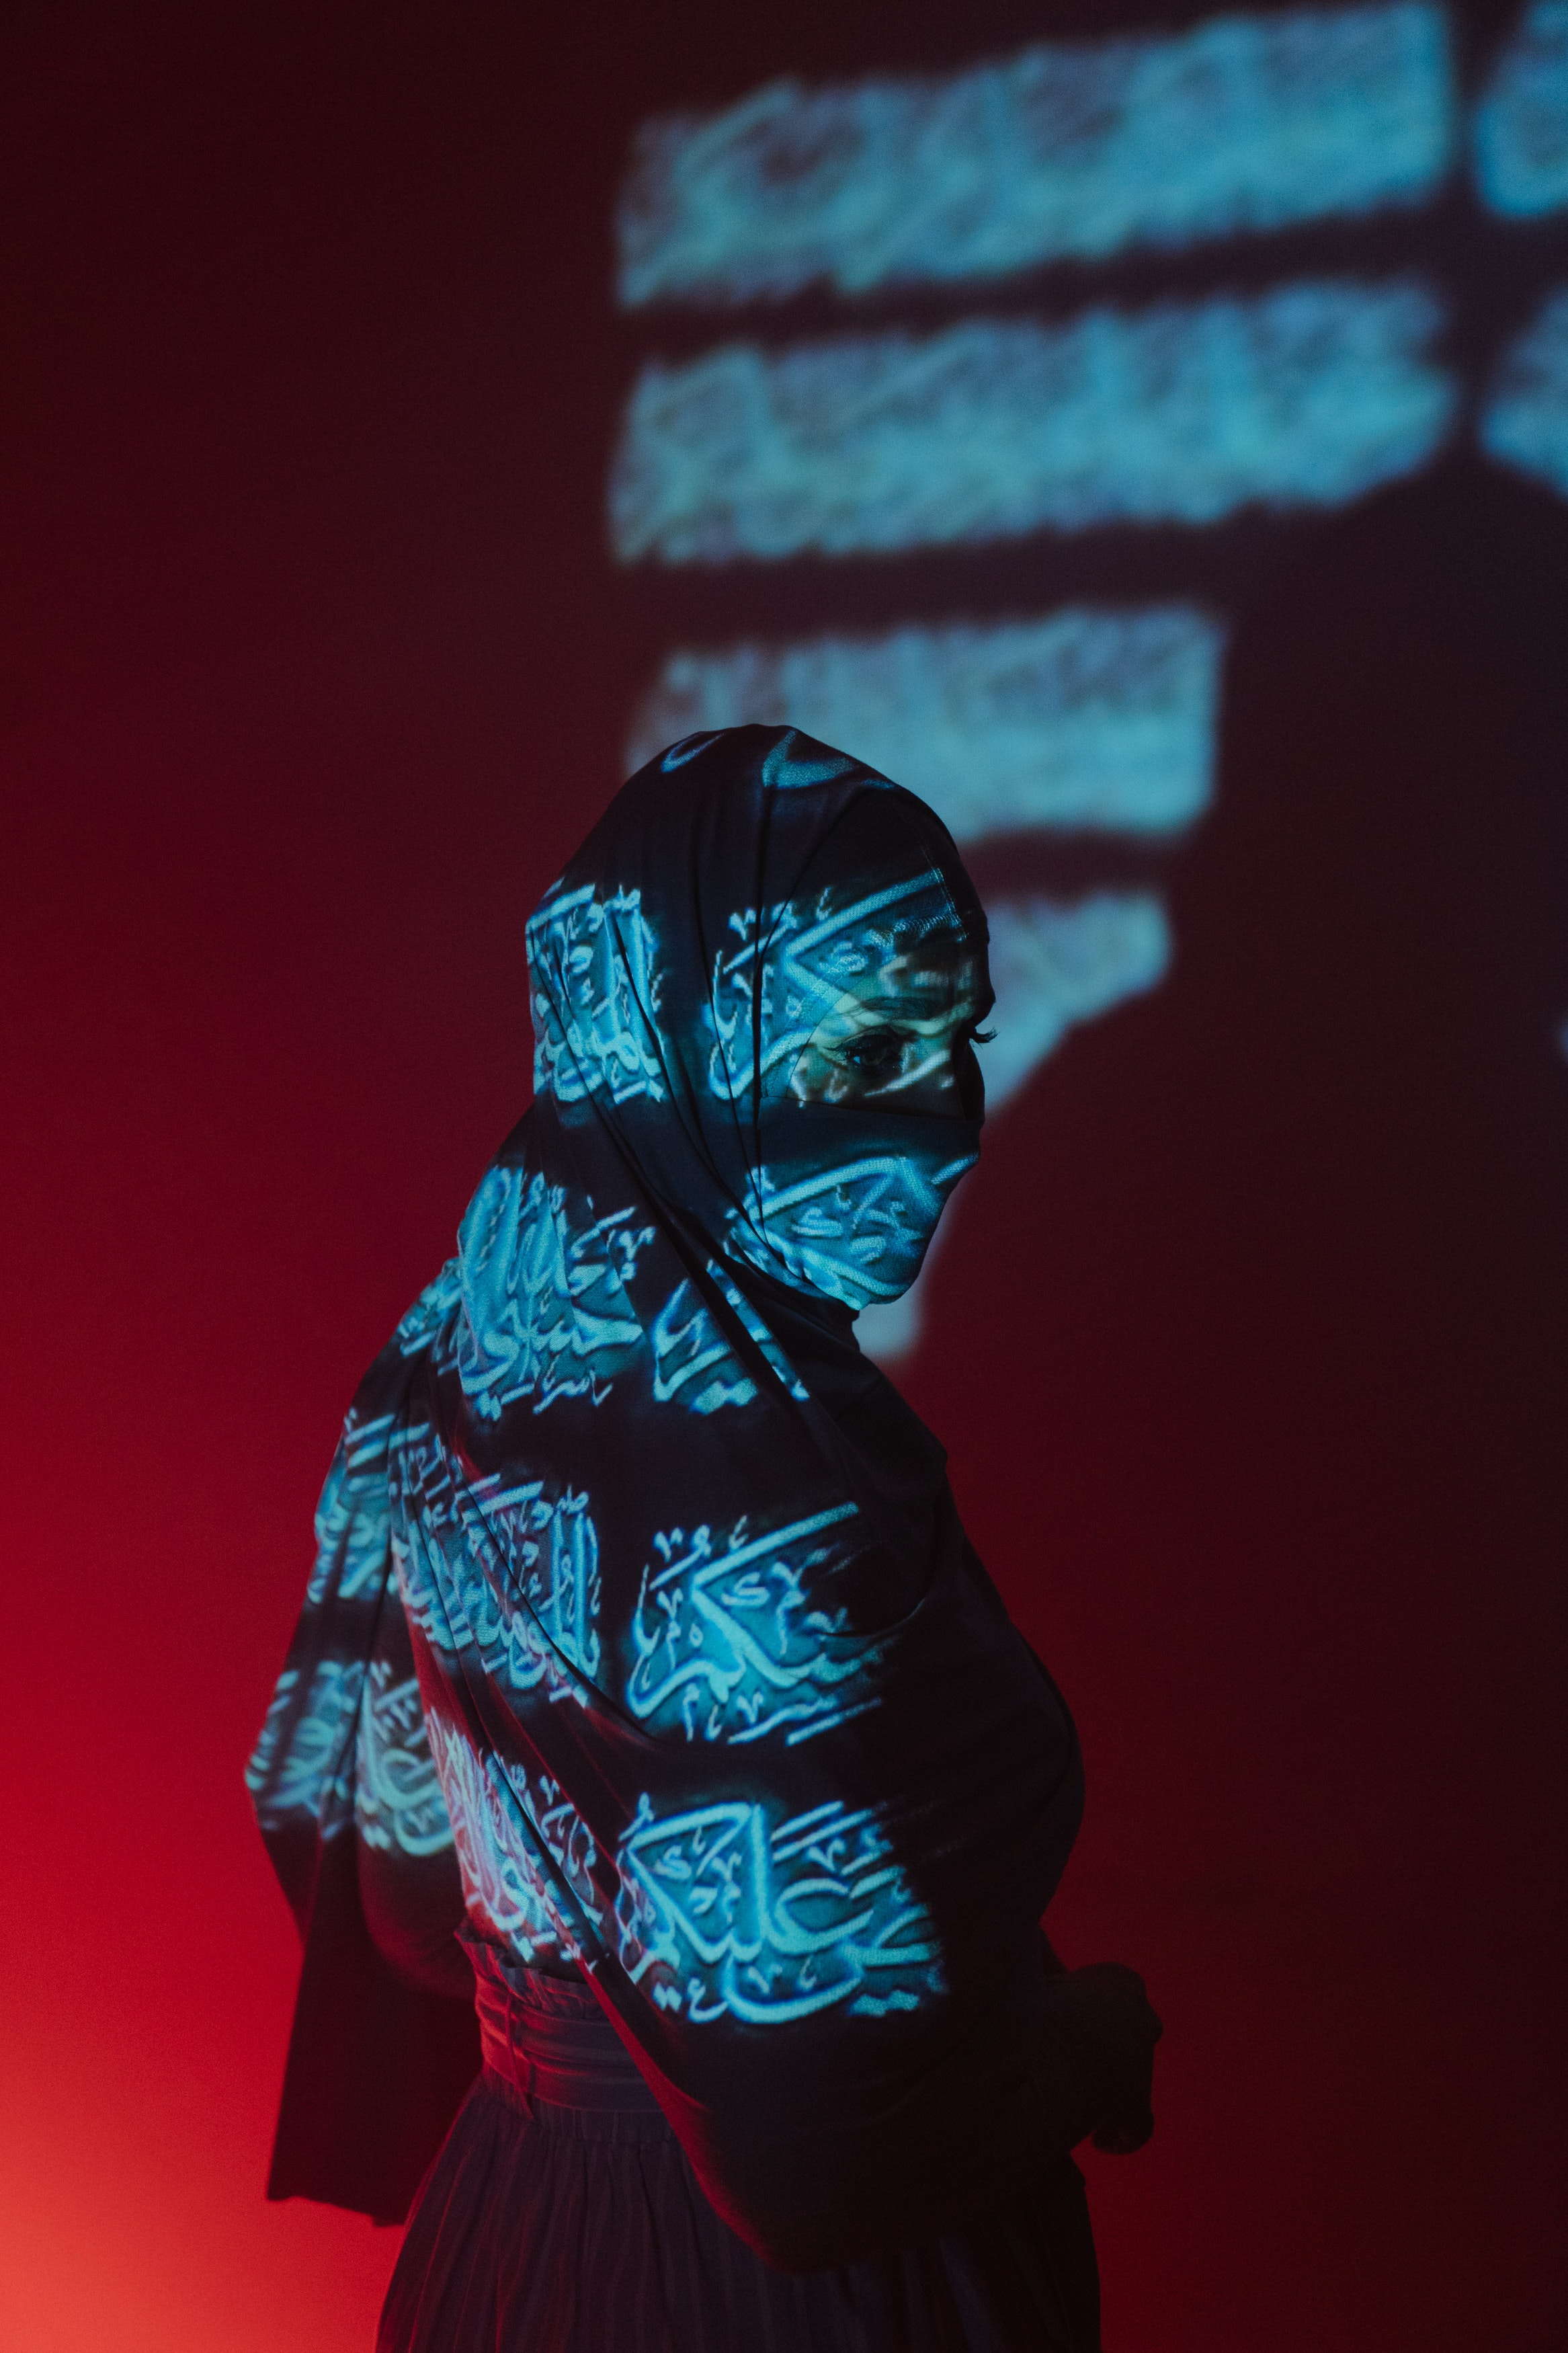
\includegraphics[width=\paperwidth,height=\paperheight]{images/pexels-cottonbro-4646235.jpg}};

\vspace*{0.7\textheight}
\begin{figure}
\begin{center}
\begin{tikzpicture}[scale=2, transform canvas={scale=2}]
  \node[draw, fill=black, fill opacity=0.7, text=black, text opacity = 1,
        rectangle split, rectangle split parts=2, line width=0,
        align=center] (a) {
\Large{\color{green} Multivariate Statistics with R}\\
\large{\color{white}\textit{Paul J. Hewson}}
\nodepart{second}

\includegraphics[width=0.1\textwidth, trim=25pt 25pt 25pt 25pt]{images/logo.png}
};
\draw[ultra thick] (a.text split west) -- (a.text split east);
\end{tikzpicture}
\end{center}
\end{figure}
%Photo by cottonbro from Pexels
\thispagestyle{empty}%

}


\begin{document}
\maketitle
\frontmatter
\setlength{\parindent}{0pt}
\setlength{\parskip}{12pt}

\pagestyle{fancy}
\lhead{Multivariate Statistics with \R}
\chead{}
\rhead{\textbf{Chapter \thechapter}}
\lfoot{STAT3401}
\cfoot{Paul Hewson}
\rfoot{\thepage}
\renewcommand{\headrulewidth}{0.4pt}
\renewcommand{\footrulewidth}{0.4pt}

\sffamily

\tableofcontents

\chapter*{Books}

Many of the statistical analyses encountered to date consist of a \emph{single response variable} and \emph{one or more explanatory variables}.  In this latter case, \emph{multiple regression}, we regressed a single response (dependent) variable on a number of explanatory (independent) variables.   This is occasionally referred to as ``multivariate regression'' which is all rather unfortunate.   There isn't an entirely clear ``canon'' of what is a multivariate technique and what isn't (one could argue that discriminant analysis involves a single dependent variable).   However, we are going to consider the simultaneous analysis of a number of related variables.   We may approach this in one of two ways.   The first group of problems relates to classification, where attention is focussed on individuals who are more alike.   In unsupervised classification (cluster analysis) we are concerned with a range of algorithms that at least try to identify individuals who are more alike if not to distinguish clear groups of individuals.   There are also a wide range of scaling techniques which help us visualise these differences in lower dimensionality.   In supervised classification (discriminant analysis) we already have information on group membership, and wish to develop rules from the data to classify future observations.  

The other group of problems concerns inter-relationships between variables.   Again, we may be interested in lower dimension that help us visualise a given dataset.   Alternatively, we may be interested to see how one group of variables is correlated with another group of variables.   Finally, we may be interested in models for the interrelationships between variables.


%Here are a few examples of multivariate analyses.   

%(a) Skulls have been recovered from an ancient burial ground.   These may come from one group, or a mixture of ethnic groups slaughtered in battle.   If we make a number of measurements on the skulls can we estimate the number of groups inovled.

%(b) Data are identified on business activity, such as national income, rate of interest, unemployment.   Can we generate a single index of ``business activity''.

%(c) A social scientist wishes to confirm the concept of ``self esteem'', based on student survey with 10 questions on attitudes.   Are the answers consistent with the existence of such a non-measurable concept.

%\subsection{Objectives}

%\begin{itemize}
%\item Grouping or sorting - objects, individuals or variables are arranged into similar clusters or groups
%\item Prediction or decision making - number of groups is known but rule(s) are required to classify individuals or objects into such groups
%\item Data reduction or simplification - relatively few indices are constructed from many measured variables
%\item Hypotheses are postulated, tested, investigated - either by analogy to univariate hypotheses or an attempt to reveal underlying influences or latent structure
%\end{itemize}

There is a reasonably established range of multivariate techniques which we will cover here.   Introductory level books include  \cite{Johnson+Wichern:2002}
%\cite{Afifi+Clark:1990} \cite{Chatfield+Collins:1980} \cite{Dillon+Goldstein:1984} \cite{Everitt+Dunn:1991} \cite{Flury+Riedwyl:1988} \cite{Johnson:1998}
%\cite{Kendall:1975} \cite{Hair+etal:1995} \cite{Hair+etal:1998} \cite{Manly:1994}

Intermediate level books include:
\cite{Flury:1997} (My personal favourite)
%\cite{Gnanadesikan:1997}
%\cite{Harris:1985} \cite{Krzanowski:2000} \cite{Krzanowski+Marriott:1994,Krzanowski+Marriott:1994II} \cite{Rencher:2002} \cite{Morrison:2005}
%\cite{Seber:1984} \cite{Timm:1975}


More advanced books:
%\cite{Anderson:1984} (I think there's a 2003 edition now) \cite{Bilodeau+Brenner:1999} \cite{Giri:2003} \cite{Mardia+etal:1979} \cite{Muirhead:1982}
\cite{Press:1982} \cite{Srivastava+Carter:1983}.


If you hunt around you will notice that the ``canon'' of multiviate methods does vary.   Some people include contingency tables and log-linear modelling, others exclude Cluster analysis.   Given that multivariate methods are particularly common in applied areas such Ecology and Psychology, it is worth a browse around library sections containing books aimed at these subjects.   It is quite possible that they will have very readable descriptions of particular techniques.   In particular, there seems to be a copious collection of books aimed at Psychologists on Factor Analysis - but there are a few caveats in the way they approach this technique and these books need to be read in the light of cautions given during lectures.



%%% Local Variables: ***
%%% mode:latex ***
%%% TeX-master: "../book.tex"  ***
%%% End: ***


\mainmatter

\chapter{Multivariate data}
\label{outline}

\section{The nature of multivariate data}
\label{overview}

We will attempt to clarify what we mean by multivariate analysis in the next section, however it is worth noting that much of the data examined is observational rather than collected from designed experiments.   It is also apparent that much of the methodology has been developed outside the statistical literature.   Our primary interest will be in examining continuous data, the only exception being categorical variables indicating group membership.   This may be slightly limiting, but we will also tend to rely on at least asymptotic approximations to (multivariate) normality, although these are not always necessary for some techniques.   The multivariate normal distribution is a fascinating subject in its own right, and experience (supplemented with some brutal transformations) indicates it is a reasonable basis for much work.   Nevertheless, there is considerable interest in robust methods at the moment and we refer to some of theseapproaches where possible.

\section{The role of multivariate investigations}
\label{role}

If we assume that linear and generalised linear models (and their descendants) are the mainstay of statistical practice, there is a sense in which most statistical analysis is multivariate.   However, \emph{multivariate analysis} has come to define a canon of methods which could be characterised by their use of the dependence structure between a large number of variables.   This canon has not yet been firmly established; we attempt one definition of it here but omit some methods others would include and include some methods others would omit.   We would suggest that multivariate analysis has either the units as a primary focus, or involves an assessment primarily of the variables.   When considering the units, we usually refer to techniques for classification; supervised classfication if we already understand the grouping and unsupervised classification where we have no \textit{a priori} knowledge of any groupings within our observed units.   The multivariate methodology at the core of supervised classification is discriminant analysis, although the machine learning community has developed many other approaches to the same task.  We will consider these techniques in the light of hypothesis tests (Hotelling's T$^{2}$ test and Multivariate Analysis of Variance) which might help us determine whether groupings within our data really are distinct.   Unsupervised classification has traditionally been associated with cluster analysis, a wide range of algorithms which attempt to find structure in data.   It is perhaps cluster analysis that is the most often contested component of our multivariate canon - some authorities prefer approaches based less on automated algorithms and rather more on statistical models and would argue for approaches such as mixture models and perhaps latent class analysis.   Given the reliance of cluster analysis on distance measures, we will also consider scaling techniques as a method of visualising distnace.   

In considering the relationship between variables, we will spend some time exploring principal components, the most misused of all multivariate techniques which we consider primarily as a projection technique.   Some coverage will also be given to canonical correlation, an attempt to understand the relationship between two sets of variables.   Finallly, we will consider factor analysis, a much contested technique in statistical circles but a much used one in applied settings.

In order to make some sense of these techniques, we will present a brief overview of linear algebra as it pertains to the techniques we wish to explore, and will present some properties of the multivariate normal distribution.



%\chapter{Presenting Multivariate Data}

\section{Summarising multivariate data (presenting data as a matrix, mean vectors, covariance matrices}
\label{summary}


A number of datasets will be used thoughout the course, where these are not available within R itself they will be posted in the student portal.  For now, consider the \emph{USArrests} data.  This was published by McNeil, D. R. (1977) ``Interactive Data Analysis'', Wiley, and gives Arrest rates in 1973 (derived from World Almanac and Book of facts 1975.  and Urban population rates derived from Statistical Abstracts of the United States 1975.  We therefore consider data on  ``Murder'' (arrests per 100,000), Assault (arrests per 100,000), Rape (arrests per 100,000) and the percentage of the population living in urban areas in each state. 

\subsection{Data display}

A matrix is a convenient way of arranging such data.

\singlespacing
\begin{displaymath}
\begin{array}{lcccc}
....................State & Murder & Assault & Rape &  UrbanPop(\%)\\
\end{array}
\end{displaymath}
\begin{displaymath}
\left[ \begin{array}{lrrrr}
Alabama       &   13.2  &   236  &     21.2 &  58\\
Alaska         &  10.0   &  263  &    44.5 & 48\\
Arizona        &   8.1  &   294   &    31.0 &  80\\
Arkansas     &     8.8 &    190  &     19.5 &  50\\
California    &    9.0  &   276  &     40.6 & 91\\
Colorado       &   7.9  &   204  &     38.7 & 78\\
Connecticut   &    3.3  &   110    &   11.1 & 77\\
Delaware      &    5.9  &   238  &     15.8 & 72\\
Florida       &   15.4  &   335   &    31.9 & 70\\
Georgia     &     17.4  &   211    &   25.8 & 60\\
Hawaii       &     5.3  &    46    &   20.2 & 83\\
$\ldots$ & $\ldots$ & $\ldots$ & $\ldots$ \\
\end{array}
\right]
\end{displaymath}
\onehalfspacing

Note in total that there are 50 states, (this display had been cut off after the 11th row, Hawaii), and that there are four variables.   Have a look at the USArrests data itself, and the associated helpfile:

\begin{verbatim}
> ?USArrests
> summary(USArrests)
> USArrests
\end{verbatim}


\section{Graphical and dynamic graphical methods}
\label{eda}



\subsection{Chernoff's Faces}

One of the more charismatic ways of presenting multivariate data was proposed by Chernoff, H. (1973) ``The use of faces to represent statistical association'', JASA, 68, pp 361-368. (see www.wiwi.uni-bielefeld.de/~wolf/ for the R code to create these).   If you have loaded the mvmmisc.R file, you can get these by typing:

\begin{verbatim}
> faces(USArrests}
\end{verbatim}


\begin{figure}
\begin{center}
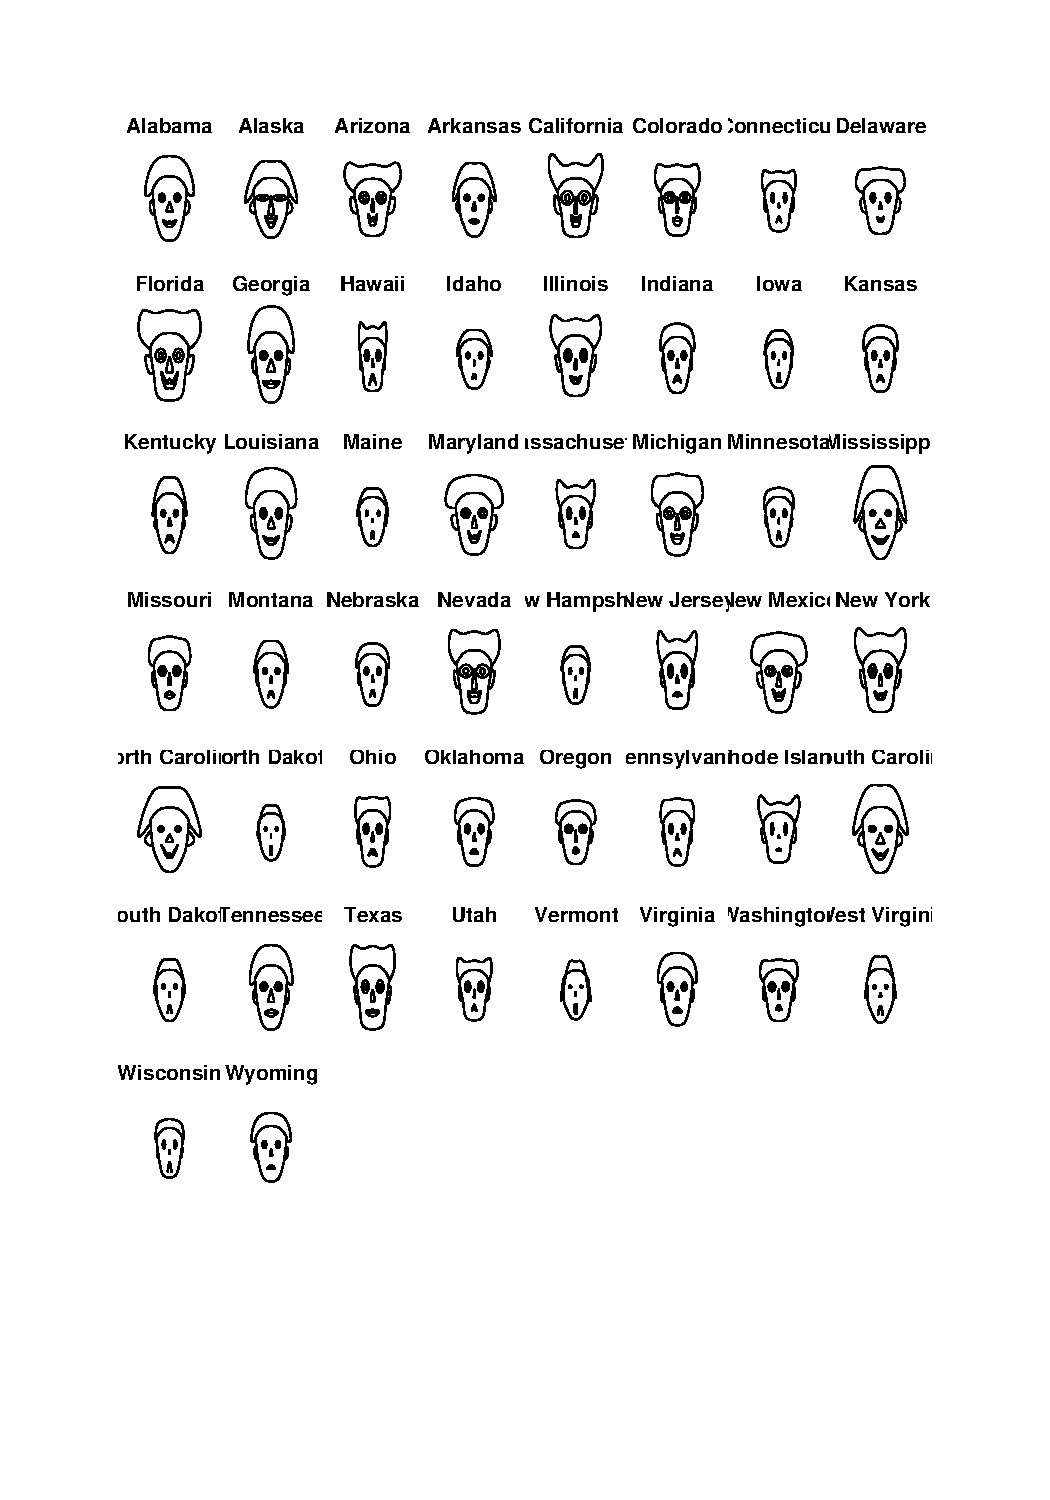
\includegraphics[width = 0.6\textwidth]{images/faces}
\caption{US Arrest data presented as Chernoff's faces}
\end{center}
\end{figure}

However, there are more useful ways of investigating multivariate data.   Slightly less wild, there are star plots, which depict the data as beams.   There are as many beams as there are variables, and the length of the beam reflects the value of the variable.

\singlespacing
\begin{verbatim}
> stars(USArrests)
\end{verbatim}
\onehalfspacing


\subsection{Scatterplots, pairwise scatterplots (draftsman plots)}

Scatterplots should already be familiar as a means of exploring the relationship between two variables.

\singlespacing
\begin{verbatim}
> attach(USArrests)
> plot(Murder, Assault)
> par(las = 1) ## Horizontal axis units on y axis
> plot(Murder, Assault, main = "Scatter plot", pch = 16) 
> detach(USArrests)
\end{verbatim}
\onehalfspacing

\begin{figure}
\begin{center}
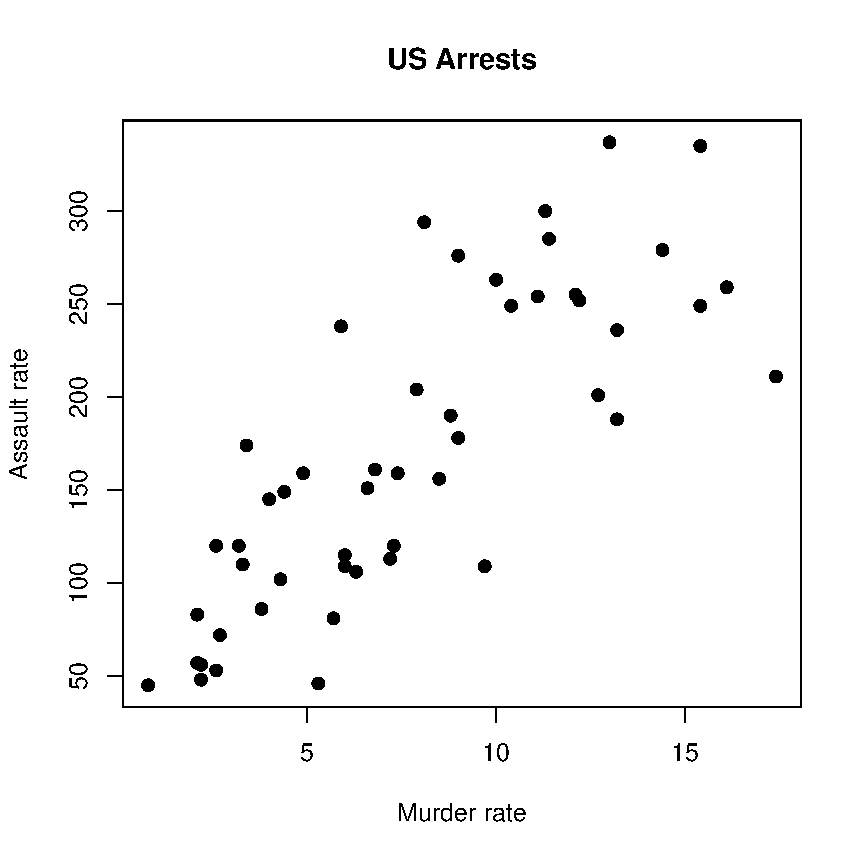
\includegraphics[width = 0.4\textwidth]{images/scatter}
\caption{Scatter plot of Murder rate against Assault rate for US States in 1973}
\end{center}
\end{figure}


However, we have more than two variables of interest.   A set of pairwise scatterplots (sometimes called a draftsman plot) may be of use:

\singlespacing
\begin{verbatim}
> pairs(USArrests, pch = 16)
\end{verbatim}
\onehalfspacing

\begin{figure}
\begin{center}
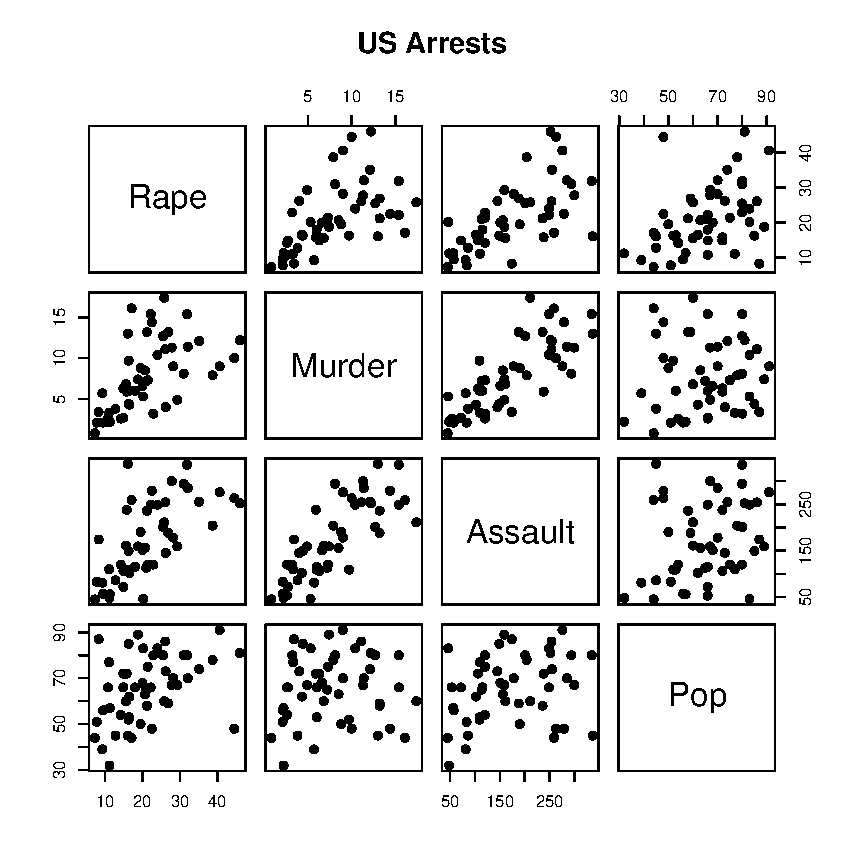
\includegraphics[width = 0.5\textwidth]{images/pairs}
\caption{Pairwise scatter plots for three US arrest rates and percent of population living in Urban areas}
\end{center}
\end{figure}

There other useful functions available.   For example what does \texttt{splom} do?    (Look up \texttt{>?splom}).

\singlespacing
\begin{verbatim}
> library(lattice)
> splom(~USArrests)
\end{verbatim}
\onehalfspacing


\subsection{Optional: 3d scatterplots}

This bit is optional: feel free to have a go if you want to find out about installing R libraries.   

There are facilities in R for making 3d effect scatterplots: you need to download and install an additional library, and when you load the library you need to tell R where to find it.   It is just possible to envisage the three dimensions on the printed page.

\singlespacing
\begin{verbatim}
> install.packages("scatterplot3d", lib = "u:/STAT3401/mvm")
> library(scatterplot3d, lib.loc = "u:/STAT3401/mvm/")
> data(trees)
>  s3d <- scatterplot3d(USArrests[,-3], type="h", highlight.3d=TRUE,
      angle=55, scale.y=0.7, pch=16, main = "USArrests")
\end{verbatim}
\onehalfspacing

\begin{figure}
\begin{center}
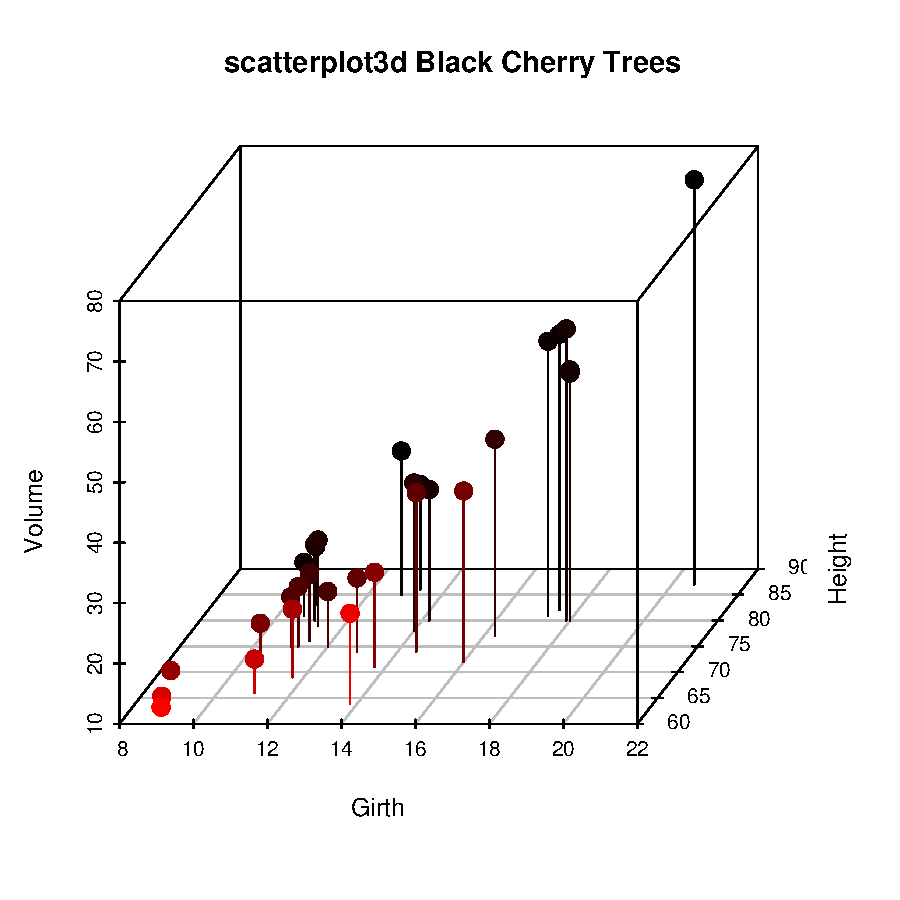
\includegraphics[width = 0.4\textwidth]{images/scat3d}
\caption{3d scatterplot of US arrests}
\end{center}
\end{figure}


\subsection{Other methods}

Other useful methods will be considered in the lab-session, such as glyphs and arrows.   For example there is a rather simple glyph plot available here:

\begin{verbatim}
glyphs(Assault, Murder, Rape, UrbanPop)
\end{verbatim}

The idea of the glyph is that two of the variables are represented as the x and y co-ordinates (as usual), but a futher variable can be represented by the angle of the arrow, and a fourth variable as the length of the arrow.

Interactive graphics offer these facilities, and many more.   There are programs such as GGobi (\texttt{www.ggobi.org}) which allow extensive multivariate investigation such as linked / brushed plots and ``grand tours''.   

\subsection{Profiles}

Just as much ingenuity was extended before modern colour systems.   Another approach is Andrews Curves, described as a function between $-\pi < t < \pi$


\begin{displaymath}
f_{x}(t) = x_{1}/\sqrt 2 + x_{2} \sin 2 + x_{3} \cos t + x_{4} \sin 2t + x_{5} \cos 2t + \ldots
\end{displaymath}

\begin{figure}
\begin{center}
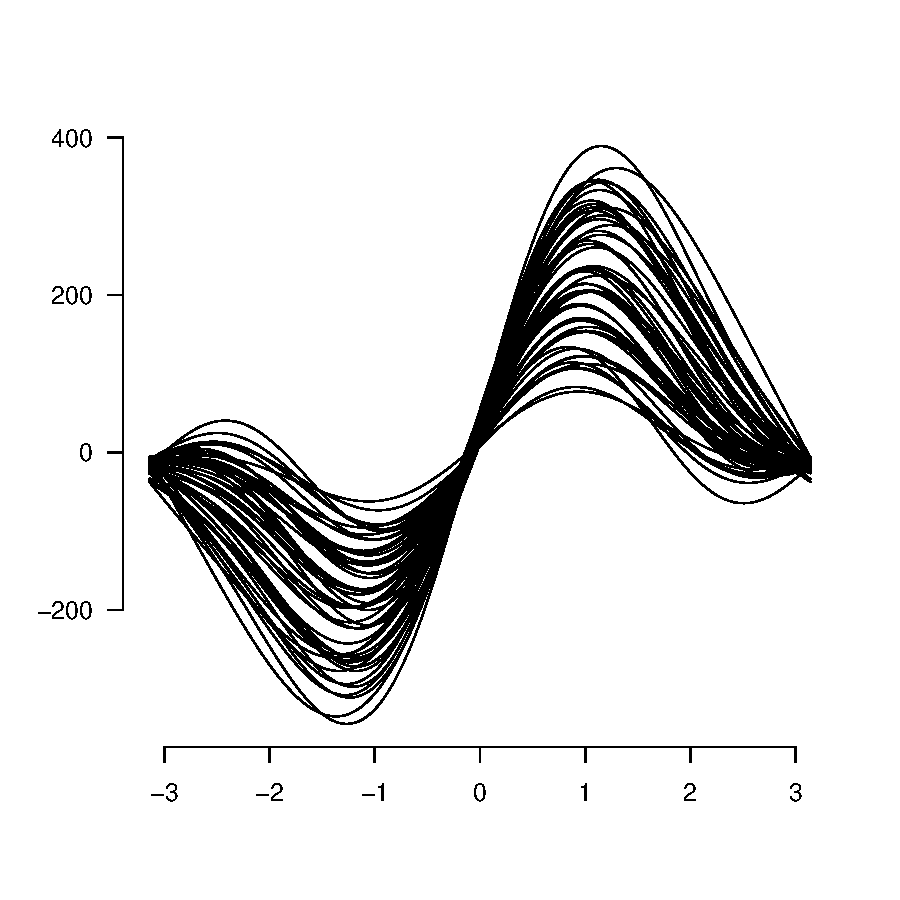
\includegraphics[width = 0.5\textwidth]{images/andrews}
\caption{Andrews Curves of US arrests data}
\end{center}
\end{figure}

You may like to consider at some stage (perhaps not today) how you could write an R function that plots Andrew's curves?   (there's a function in the \texttt{mvmmisc.R} file).

Try creating a matrix of data values from Fisher's Iris data, and a column of species names.   Then call up the andrews curves function:

\singlespacing
\begin{verbatim}
> iris.data <- iris[,-5]
> iris.species <- iris[,5]
> andrews.curves(iris.data, iris.species)
\end{verbatim}
\onehalfspacing


However, a simpler profile plots is available from the MASS library:

\singlespacing
\begin{verbatim}
> library(MASS)
> parcoord(USArrests)
\end{verbatim}
\onehalfspacing

The idea is that not only are the values of each individual variable represented, but also the patterns of different individuals can be seen.

If you now try looking at Fisher's Iris data (the [,-5] drops the species column which is a factor and cannot be plotted)

\singlespacing
\begin{verbatim}
> parcoord(iris[,-5])
\end{verbatim}
\onehalfspacing

You can also tell \texttt{parcoord()} to colour the profiles in according to the species.

\singlespacing
\begin{verbatim}
> parcoord(iris[,-5], col = as.numeric(iris[,5]))
\end{verbatim}
\onehalfspacing


\section{Animated exploration}

\begin{figure}
\begin{center}
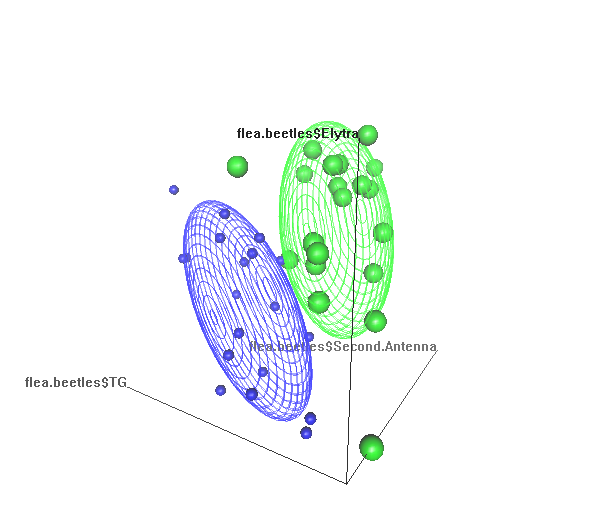
\includegraphics[width = 0.5\textwidth]{images/rgl}
\caption{rgl animated view of first three variables of flea beetle data}
\label{rgl}
\end{center}
\end{figure}

This shows an rgl with ellipsoids.


%\section{Dimension reduction}
%\label{dr}
%\section{Measures of distance}
%\label{distance}



%\section{Exercises}

%Hopefully the above examples, based on the USArrests data, give you some ideas as to how we start to visualise multivariate data.   We will consider more specialised methods (such as biplots and other projection methods) as the course progresses.   This week, you are strongly encouraged to consider how you could visualise the following datasets (all within R).

%\singlespacing
%\begin{itemize}
%\item attitude (survey of employees in different departments of a firm)
%\item longley (economic data)
%\item swiss (fertility and socio-economic data)
%\item USJudgeRatings (how lawyers rate judges in the US)
%\end{itemize}
%\onehalfspacing

You can use the help system to find more information on the datasets (e.g. type \texttt{> ?longley}).
%
%\fbox{Consider suitable methods for presenting these data.}

%%% Local Variables: ***
%%% mode:latex ***
%%% TeX-master: "../book.tex"  ***
%%% End: ***





\chapter{Measures of distance}
\label{dist}

We take a little time out here to consider some ideas regarding multivariate distance and introduce some properties of multivariate distance matrices.   These concepts are most obviously relevant when considering multivariate technique such as cluster analysis and scaling methods, where we wish to examine the difference between individuals.   In doing this, we need to find some definition of the concept of ``difference between individuals'', and will therefore consider a range of proximity measures.   We also provide some discussion of difference between variables.   These are currently important concepts in bio-informatic applications but earlier work in multivariate statistics involved consideration of variables which may be carrying similar information where cluster analysis of variables could be used as a preliminary data analytical exercise.   We start by considering one particular measure, the Mahalanobis distance.

\section{Mahalanobis Distance}
\label{standarddist}

The Mahalanobis distance has an important role in multivariate theory, albeit this is often an implied consideration rather than an explicit one.   For example, development of forms of discriminant analysis considered in chapter \ref{discriminant} involve this measure.   There are however a number of important distributional properties of the Mahalanobis distance which could be more used in determining multivariate normality.    It should be noted that use of standard distance requires a parametric view of the world, and in particular it is most applicable for symmetric distributions.   We follow \cite{Flury:1997} in providing the following exposition of the standard distance.  

Firstly, if we consider the \emph{univariate} standard distance we see that this is a measure of the absolute distance between two observations in units of their standard deviation.
\marginnote{The standardisation is important; this measure it is invariant under non-degenerate linear transformations.   A univariate example would be given by considering $Y = \alpha  + \beta X$, where $\beta \neq 0$ and $\alpha$ are fixed constants.   Consider transforming $x_{1}$ and $x_{2}$ to $y_{i} = \alpha + \beta x_{i}; i = 1,2$. Then considering the standard distance between these two transformed variables we find:

\begin{eqnarray*}
d(y_{1},y_{2}) &=& \frac{|y_{1} - y_{2}|}{\sqrt{var(Y)}}\\
 &=&  \frac{|\beta(x_{1} - x_{2}|)}{\sqrt{\beta^{2}\sigma^{2}}}\\
 &=& d(x_{1},x_{2})
\end{eqnarray*}
}
Given $X$, a random variable with mean $\mu$ and variance $\sigma^{2} > 0$, the \emph{standard distance}, between two numbers $x_{1}$ and $x_{2}$ is defined as follows:

\begin{displaymath}
d(x_{1}, x_{2}) = \frac{|x_{1} - x_{2}|}{\sigma}
\end{displaymath}

\marginnote{Where $\sigma = 1$, this standard distance is the same as the Euclidean distance given later in section \ref{euclidean}}.

The univariate standard distance has a straightforward generalisation to a multivariate setting.   Considering now two vectors  $\boldsymbol{x}_{1}$ and $\boldsymbol{x}_{2}$, with a common covariance matrix $\boldsymbol{\Sigma}$ the multivariate standard distance is given by:

\begin{displaymath}
d(\boldsymbol{x}_{1},\boldsymbol{x}_{2}) = \sqrt{(\boldsymbol{x}_{1} - \boldsymbol{x}_{2})^{T}\boldsymbol{\Sigma}^{-1}(\boldsymbol{x}_{1},\boldsymbol{x}_{2}) }
\end{displaymath}

Depending on whichever textbook is consulted, this multivariate standard distance may be referred to as the \emph{statistical distance}, the \emph{elliptical distance} or the \emph{Mahalanobis distance}.   \cite{Flury:1997} notes that the squared Mahalanobis distance $d(\boldsymbol{x}_{1},\boldsymbol{x}_{2})^{2}$ is sometimes simply referred to as the Mahalanobis distance, although it is not a valid distance measure.   We refer here to the multivariate standard distance,  $d(\boldsymbol{x}_{1},\boldsymbol{x}_{2})$ as the Mahalanobis distance, and where necessary, to  $d(\boldsymbol{x}_{1},\boldsymbol{x}_{2})^{2}$ as the \emph{squared} Mahalanobis distance.


It is worth noting that this measure was originally proposed by
\cite{Mahalanobis:1930} as a measure of distance between two populations:

\begin{displaymath}
\Delta(\boldsymbol{\mu}_{1},\boldsymbol{\mu}_{2}) = \sqrt{(\boldsymbol{\mu}_{1} - \boldsymbol{\mu}_{2})^{T}\boldsymbol{\Sigma}^{-1}(\boldsymbol{\mu}_{1},\boldsymbol{\mu}_{2}) }
\end{displaymath}
which has an obvious sample analogue as the distance between two mean vectors:

\begin{displaymath}
\Delta(\boldsymbol{\bar{x}}_{1},\boldsymbol{\bar{x}}_{2}) = \sqrt{(\boldsymbol{\bar{x}}_{1} - \boldsymbol{\bar{x}}_{2})^{T}\boldsymbol{S}^{-1}(\boldsymbol{\bar{x}}_{1},\boldsymbol{\bar{x}}_{2}) }
\end{displaymath}
where $\boldsymbol{S}$ is the pooled estimate of $\boldsymbol{\Sigma}$ given by $\boldsymbol{S} = \left[ (n_{1}-1) \boldsymbol{S}_{1} +  (n_{2}-1) \boldsymbol{S}_{2} \right] / (n_{1} + n_{2} - 2)$.

Here, we are going to consider the distance between $\boldsymbol{x}$, a vector of random variables with mean $\boldsymbol{\mu}$ and covariance matrix $\boldsymbol{\Sigma}$ and its mean:

\begin{displaymath}
\Delta(\boldsymbol{x},\boldsymbol{\mu}) = \sqrt{(\boldsymbol{x} - \boldsymbol{\mu})^{T}\boldsymbol{\Sigma}^{-1}(\boldsymbol{x},\boldsymbol{\mu}) }
\end{displaymath}
and clearly we can find a sample analogue by estimating $\boldsymbol{\mu}$ by $\hat{\boldsymbol{x}}$ and $\boldsymbol{\Sigma}$ by $\boldsymbol{S} = \frac{1}{n-1} \boldsymbol{X}^{T}\boldsymbol{X}$.  We note that in \textbf{R}, the \verb+mahalanobis()+ function is intended to returns the \emph{squared} multivariate distance between a matrix $\boldsymbol{X}$ and a mean vector $\boldsymbol{\mu}$, given a user-supplied covariance matrix $\boldsymbol{\Sigma}$, i.e. we wish to calculate: 

\begin{displaymath}
d(\boldsymbol{x}_{i},\hat{\boldsymbol{\mu}})^{2} 
= (\boldsymbol{x}_{i} - \hat{\boldsymbol{\mu}})^{T}
\hat{\boldsymbol{\Sigma}}^{-1}
(\boldsymbol{x}_{i} - \hat{\boldsymbol{\mu}}) 
\end{displaymath}

We could also consider the Mahalanobis angle $\theta$ between two vectors at the origin:

\begin{displaymath}
\cos \theta = \frac{\boldsymbol{x}_{1}^{T} \boldsymbol{S}^{-1} \boldsymbol{x}_{2}}
{d(\boldsymbol{x}_{1},\boldsymbol{0})d(\boldsymbol{x}_{2},\boldsymbol{0})}
\end{displaymath}

This can be extracted from within $\boldsymbol{R}$ using the following:

\begin{Schunk}
\begin{Sinput}
> mahangle <- function(x1, x2, covmat){
+   zero <- vector("numeric", length(x1) )  
+   num <- t(x1) %*% solve(covmat) %*% x2
+   denom <- sqrt(mahalanobis(x1, zero, covmat)) * 
+      sqrt(mahalanobis(x2, zero, covmat)) 
+   angle <- acos(num / denom)
+   return(angle)
+ }
\end{Sinput}
\end{Schunk}

\subsection{Distributional properties of the Mahalanobis distance}

Remembering that where $z_{1}, \ldots, z_{p} \sim N(0,1)$, if we form $y = \sum_{j=1}^{p} z_{j}^{2}$ then $y \sim \chi_{p}^{2}$ \citep{Bilodeau+Brenner:1999}; for multivariate normal data, with $p$ variables, the squared Mahalanobis distance can be considered against a $\chi_{p}^{2}$ distribution:

\begin{equation}
(\boldsymbol{x}_{i} - \hat{\boldsymbol{\mu}})^{T}
\hat{\boldsymbol{\Sigma}}^{-1}
(\boldsymbol{x}_{i} - \hat{\boldsymbol{\mu}}) = \boldsymbol{z}^{T}\boldsymbol{z} \sim \chi^{2}_{p}
\end{equation}

This immediately affords one method for assessing multivariate normality, quantiles of the Mahalanobis distance of $\boldsymbol{x}_{i}$, $i = 1, \ldots, n$ with respect to $\boldsymbol{\mu}$ can be plotted against quantiles of the $\chi^{2}_{p}$ distribution as an assessment of multivariate normality.

\begin{figure}
\begin{center}
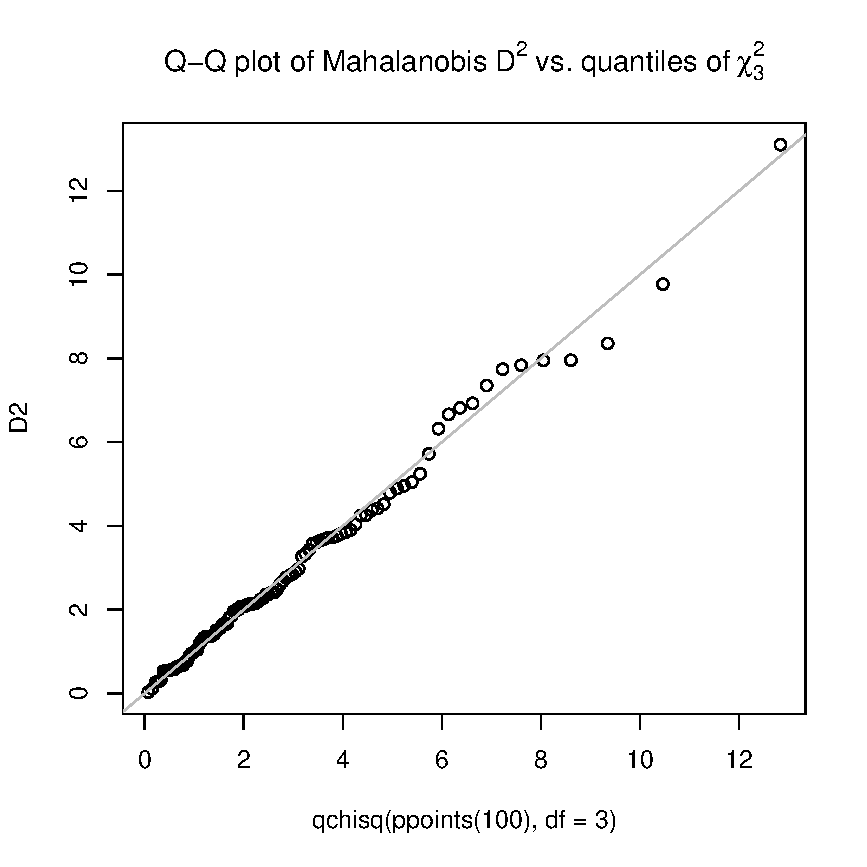
\includegraphics[width = 0.5\textwidth]{images/DistChiPlot}
\caption{QQ plot of squared Mahalahobis distance plotted against $\chi^{2}$ distribution}
\label{qqchimahlanobis}
\end{center}
\end{figure}

We can also define contours as a set of points of equal probility in terms of equal Mahalanobis distance:

\begin{equation}
(\boldsymbol{x}_{i} - \hat{\boldsymbol{\mu}})^{T}
\hat{\boldsymbol{\Sigma}}^{-1}
(\boldsymbol{x}_{i} - \hat{\boldsymbol{\mu}}) = \boldsymbol{z}^{T}\boldsymbol{z} = c^{2}
\end{equation}

for any constant $c > 0$.  We will also find later in section \ref{mahalpca} that the squared Mahalanobis distance is equivalent to the sum of squared prinicipal component scores.   However, this chapter on distance is implicitly geared towards presentations in the chapter \ref{clustan} on cluster analysis as well as  chapter \ref{mds} on scaling methods.   In that context it is worth noting that Mahalanobis distance is rarely used in cluster analysis, certainly \cite{Kendall:1975} points out its limitations in this context.  Sporadic reports in the literature include \cite{Maronna+Jacovkis:1974} who report use of a particular clustering algorithm, $k$-means, with the Mahalanobis distance whereas \cite{Gnanadesikan+etal:1993} use it with hierarchical cluster analysis.   This latter work may illustrate one of the difficulties in using the Mahalanobis distance in the requirement to assume a common covariance.     However, whilst not proposing it's use in an automatic clustering algorithm, \cite{Atkinson+etal:2004} report use of Mahalanobis distance within the forward search to reliably identify subgroups within the data.   They propose a small modification to the Mahalanobis distance for use in cluster analysis as follows.   The Mahalanobis distance is multiplied by $(|\hat{\boldsymbol{\Sigma}}^{-1}_{k}|^{1/2})^{r}$ for group $k$.   Where $r=0$ we have the usual distance, when $r=1$ we have what they call the \emph{standardised} Mahalanobis distance which eliminates the different variance between groups.

Having provided an overview of one distributionally important distance measure, before considering further measures we consider a few definitions.   \cite{Flury:1997} notes that the squared Mahalanobis distance does not satisfy the axioms of distance.

\section{Definitions}
\label{distdefinitions}

We now formalise our idea of a proximity measure.  This term encapsulates both similarity and disssimilarity measures which have the obvious interpretation (measuring similarity and dissimilarity between entities), and can be found from each other by means of an appropriate monotonic transformation.   We usually assume that these measures are symmetic.

A \emph{distance} can be defined as a function $d(\cdot)$ that satisfies the following properties:

\begin{itemize}
\item[(1)] Non-negative, that is $d(\boldsymbol{x},\boldsymbol{y}) \geq 0$ for all $\boldsymbol{x},\boldsymbol{y} \in \mathbb{R}^{p}$ and 
\item[(2)] Identified, that is $d(\boldsymbol{x},\boldsymbol{x}) = 0$ for all $\boldsymbol{x} \in \mathbb{R}^{p}$;
\item[(3)] Symmetric, that is $d(\boldsymbol{x},\boldsymbol{y}) = d(\boldsymbol{y},\boldsymbol{x})$ for all $\boldsymbol{x},\boldsymbol{y} \in \mathbb{R}$;
\end{itemize}

In addition to satisfying these three properties, a \emph{metric} also satisfies the following two properties:
\begin{itemize}
\item[(4)] Definite, that is $d(\boldsymbol{x},\boldsymbol{y}) = 0$ if and only if $\boldsymbol{x} = \boldsymbol{y}$ for all $\boldsymbol{x},\boldsymbol{y} \in \mathbb{R}^{p}$;
\item[(5)] Triange inequality $d(\boldsymbol{x},\boldsymbol{y}) + d(\boldsymbol{y},\boldsymbol{z}) \geq d(\boldsymbol{x},\boldsymbol{z})$ for all $\boldsymbol{x},\boldsymbol{y},\boldsymbol{z} \in \mathbb{R}$  
\end{itemize}


It is worth noting that it is possible to compute a similarity measure, often denoted $s$, where $0 \leq S \leq 1$.   A \emph{similarity} function $s(\cdot,\cdot)$ satisfies (1) non-negativity $s(\boldsymbol{x}, \boldsymbol{y}) \geq 0$, (2) symmetry $S(\boldsymbol{x},\boldsymbol{y}) = s(\boldsymbol{y},\boldsymbol{x})$ as well as:

\begin{itemize}
\item[(3)] $s(\boldsymbol{x}, \boldsymbol{y})$ increases in a monotone fashion as $\boldsymbol{x}$ and $\boldsymbol{y}$ become more similar.   A \emph{dissimilarity} function satisfies the first two but clearly 3 is reversed, i.e. it decreases as  $\boldsymbol{x}$ and $\boldsymbol{y}$ become more similar.  
\end{itemize}

Dissimilarity is the opposite of similarity, therefore any monotonically decreasing transformation of $s$ can provide a dissimilarity measure.   The most obvious tranform would be to take $d = 1 - s$ but we will consider a few alternatives later.

\section{Distance between points}
\label{pointdistance}

Two \textbf{R} packages are needed to provide most of the distance functions considered here.   In addition to the default \verb+stats+ library, which provides the \verb+dist()+ function, we require the \verb+cluster+ package for the \verb+daisy()+ function.   Some further correlation based measures can be found in the \verb+Dist()+ function in the \verb+amap+ package as well as \verb+BioBase+ from Bioconductor.

We now consider a range of ways in which a multivariate distance can be measured.  In conducting an analysis, some decision needs to be made as to whether to scale variables, or whether to remove highly correlated variables from the analysis.   For example, \cite{Gnanadesikan:1997} gives an artificial example which illustrates how rescaling variables can subsequently alter impression of groupings.


\subsection{Quantitative variables - Interval scaled}
\label{distancequant}

It is reasonably straightforward to suggest a number of dissmilarity measures $d_{ij}$ which measure the distance between individual $i$ and $j$.

%\begin{itemize}
%\item 
\subsection{Euclidean distance}.
\label{euclidean}

The Euclidean distance, or the $l_{2}$ norm, is perhaps the most commonly used distance measure.   As mentioned in section \ref{standarddist}, this distance could be considered simply as the Mahalanobis distance where $\sigma$ = 1.   Especially in the context of cluster analysis, where we hope to identify distinct sub-groups within the data, it is not clear how we might determine the covariance matrix hence the Mahalanobis distance has seen little use.   The Euclidean distance, which is quite simply the square root of the squared distance between any two vectors, which can be quite simply interpreted as the physical distance between two $p$-dimensional points is also a convenient measure to understand.  Formally, we can express this measure as:

\begin{displaymath}
\label{euclideanF}
d_{ij} =  \left( \Sigma_{k=1}^{p} (x_{ik} - x_{jk})^2 \right)^{\frac{1}{2}}
\end{displaymath}

where we are trying to measure the distance between observations in row $i$ and row $j$, in other words $x_{ik}$ is the $k$th observation in row $i$, and $x_{jk}$ is the corresponding $k$th observation in row $j$.   Euclidean distance can be readily calculated in \textbf{R} using the \verb+dist()+ function with the default \verb+method = "euclidean"+, as well as by \verb+daisy()+ with the default \verb+metric = "euclidean"+, although in \verb+daisy()+ it is possible to standardise the data within the calculations by adding \verb+stand = TRUE+ to the function call.
 

\subsection{Scaled Euclidean distance}
\label{scaledeuclidean}

It is possible to introduce a suitable weight $w_{k}$ such as the inverse of the standard deviation of the $k$th variable, i.e. $w_{k} = s_{k}^{-1}$, or even the inverse of the range of the data.

\begin{displaymath}
\label{scaledeuclideanF}
d_{ij} = \sqrt{\left( \Sigma_{k=1}^{p} w_{k}^{2}(x_{ik} - x_{jk})^2 \right)}
\end{displaymath}

No explicit routines are available to compute this measure, but clearly if the co-ordinates are rescaled by $\sqrt{w_{k}}$ this can be calculated implicitly.

\subsection{City Block metric}
\label{cityblock}

The City Block metric, formally referred to as an $l_{1}$ norm, measures the absolute difference between two vectors.   It is so-named because it measures the distance between two points in terms of movements parallel to the axis and therefore resembles the distance between two points in a city.   \cite{Krause:1975} (who had obviously never been in a London taxi) called this distance the \emph{taxicab} distance, \cite{Brandeau+Chiu:1988} used the term \emph{rectilinear}, but perhaps the most common alternative name is \emph{Manhattan}, suggested by \cite{Larson+Sadiq:1983} reflecting the famous city block layout in Manhattan.   Formally, we can express this distance as:

\begin{displaymath}
\label{cityblockF}
d_{ij} =  \left( \Sigma_{k=1}^{p} |x_{ik} - x_{jk}| \right)
\end{displaymath}

It can be calculated in R using the \verb+dist()+ function with \verb+method = "manhattan"+



\subsection{Minkowski metric}
\label{minkowski}

The Minkowski metric, or the $l_{r}$ norm, is a generalisation of the Manhattan and Euclidean distances.

\begin{displaymath}
\label{minkowskiF}
d_{ij} =  \left( \Sigma_{k=1}^{p} |x_{ik} - x_{jk}|^\lambda \right)^{1/\lambda}
\end{displaymath}

Where $\lambda = 1$ we have the Manhattan metric, where $\lambda = 2$ we have the Euclidean distance.   It can be noted that increasing $\lambda$ exaggerates dissimilar units relative to similar ones.   This metric can be calculated in R using the \verb+dist()+ function with \verb+method = "minkowski"+ but additionally requires an argument to \verb+p+ to set $\lambda$, the power of this distance.   Therefore, for example \verb+dist(x, method = "minkowski", p=2)+ gives the Euclidean distance for matrix \verb+x+. 

\subsection{Canberra metric}
\label{canberra}

The Canberra metric \citep{Lance+Williams:1966} can be regarded as a generalisation of binary dissimilarity measures, and is very sensitive to small changes close to $x_{ik} = x_{jk} = 0$.   It can be scaled by division by $p$, the number of variables to ensure it lies in the range (0,1).   Terms with zero numerator and denominator are omitted from the sum and treated as if the values were missing.

\begin{displaymath}
\label{canberraF}
d_{ij} = \left\{ \begin{array}{ll} 0 & for\ x_{ik} = x_{jk} = 0\\
  \Sigma\left( \frac{|x_{ik} - x_{jk}|}{ |x_{ik} + x_{jk}|} \right) & for\  x_{ik} \neq 0\ or\  x_{jk} \neq 0 \end{array} \right.
\end{displaymath}

This metric can be calculated in \textbf{R} using the \verb+dist()+ function with \verb+method = "canberra"+

\subsection{Czekanowski Coefficient}
\label{czekanowski}

Finally, we mention the Czekanowski Coefficient, which for continuous variables can be given as:

\begin{displaymath}
\label{czekanowskiF}
d_{ij} = 1 - \frac{2 \sum_{k=1}^{p} min(x_{ik},x_{jk})}{\sum_{k=1}^{p}(x_{ik} + x_{jk})}
\end{displaymath}

%\end{itemize}


\subsection{Distance between variables}
\label{corrdist}

We next consider a number of correlation based distance measures.   Note that when used conventionally for calculating the correlation between two variables we work with standardised columns.  In order to measure the similarity between two individuals we must therefore work with standardised rows, this may not be a sensible procedure.   For example, if variables are measured on different scales the idea of a row mean may not be clear.   There is further material in the literature questioning the use of these measures \citep{Jardine+Sibson:1971,Fleiss+Zubin:1969} and \cite{Everitt+etal:2001} note that correlation measures cannot distinguish the size of two different observations, giving the example $\boldsymbol{x}^{T}_{1} = c(1,2,3)$ and $\boldsymbol{x}^{T}_{2} = c(1,2,3)$ have correlation $\rho_{12} = 1$ yet $\boldsymbol{x}^{T}_{2}$ is three times the size of $\boldsymbol{x}^{T}_{1}$.   Nevertheless, correlation based measures have become particular popular in a bio-informatics setting where some of the noted limitations do not apply (all variables are measured on a comparable scale) and in fact it is not always clear what a row and a column mean in that application area.   

We therefore consider four four distances that can be obtained a correlation measure.  Some thought needs to be given to determining the transformation from a correlation coefficient to a distance measure.   The Pearson correlation coefficient is defined in the range $-1 \leq \rho_{ij} \leq 1$.   \cite{Everitt+etal:2001} suggest using $d_{ij} = \frac{1 - \rho_{ij}}{2}$.  \cite{Gentleman+etal:2005} suggest that it may be appropriate under some circumstances to use the absolute value of the correlation, that is $d_{ij} = 1 - |\rho_{ij}|$ which means that there will be little distance between rows having strong positive and strong negative correlation.   In terms of measuring the dissimilarity between variables, \cite{Krzanowski:2000} suggests a further alternative using  $d_{ij} = 1 - (\rho_{ij})^{2}$.   Examining pre-Bioinformatics data, \cite{Lance+Williams:1979} who compared a number of transformations and expressed a strong preference for the first transformation, and a strong disdain for the third.

It should be noted that these measures are quite badly affected by outliers.   As a result, non-parametric versions may often be preferred.   Conversely, these measures are invariant to change of location or scale transformation which is rather useful.   It should be noted in bio-informatics practice that they tend to group genes whose expression patterns are linearly related, there is some empirical support from that application for their use in a particular context.

\subsection{Pearson correlation distance}
\label{pearsondist}

\begin{displaymath}
\label{pearsondistF}
d(x_{ij},x_{ik}) = 1 - \rho_{ij} = 1 - \frac{\sum_{i=1}^{p} (x_{ij} - \bar{x}_{\cdot j}) (x_{ik} - \bar{x}_{\cdot k}}{\sqrt{\sum_{i=1}^{p} (x_{ij} - \bar{x}_{\cdot j})^{2} \sum_{i=1}^{p} (x_{ik} - \bar{x}_{\cdot k})^{2}}}
\end{displaymath}

Where data are scaled, i.e. mean centred and standardised by the variance so that $\boldsymbol{x}_{\cdot j}$ and $\boldsymbol{x}_{\cdot k}$ are $p$ variable vecotres with zero mean and unit variance the relationship between the Euclidean distance and the Pearson correlation is given by:

\begin{displaymath}
d_{ij}^{(Euclidean)} = \sqrt{2p(1-\rho_{ij})}
\end{displaymath}

The pearson based distance measure can apparently be obtained from \verb+Dist()+ in the \verb+amap+ package, where it is referred to as the ``Centred Pearson'' by specifying \verb+method = "correlation"+ in the function call.  

\subsection{Cosine correlation coefficient}
\label{cosinedist}

This is similar to the Pearson Correlation coefficient based distance measure but without the mean standardisation

\begin{displaymath}
\label{cosinedistF}
d(x_{ij},x_{ik}) = 1 - \frac{\boldsymbol{x}_{\cdot j}^{T} \boldsymbol{x}_{\cdot k}}{||\boldsymbol{x}_{\cdot j}|| ||\boldsymbol{x}_{\cdot k}||} = 1 - \frac{|\sum_{i=1}^{p} (x_{ij}) x_{ik} }{\sqrt{\sum_{i=1}^{p} x_{ij}^{2} \sum_{i=1}^{p} x_{ik}^{2}}}
\end{displaymath}


The cosine correlation based distance measure, referred to as the ``Not-centred Pearson  can be obtained from \verb+Dist()+ in the \verb+amap+ package by specifying \verb+method = "pearson"+ in the function call.    It is not clear from the help file how the correlation measure is transformed into a distance measure.

\subsection{Spearman sample correlation distance}
\label{spearmandist}

\begin{displaymath}
\label{spearmandistF}
d(x_{ij},x_{ik}) = 1 - \rho_{ij} = 
1 - \frac{\sum_{i=1}^{p} (rank(x)_{ij} - rank(\bar{x})_{\cdot j}) (rank(x)_{ik} - rank(\bar{x})_{\cdot k})}
{\sqrt{\sum_{i=1}^{p} (rank(x)_{ij} - rank(\bar{x})_{\cdot j})^{2} \sum_{i=1}^{p} ( rank(x)_{ik} - rank(\bar{x})_{\cdot k})^{2}}}
\end{displaymath}

This requires \verb+spearman.dist()+ in package \verb+bioDist+, and can be computed via \verb+Dist()+ in the \verb+amap+ package with a call containing \verb+method="spearman"+.


\subsection{Kendall's $\tau$ sample correlation distance}
\label{kendalltaudist}

\begin{displaymath}
\label{kendalltaudistF}
d(x_{ij},x_{ik}) = 1 - \tau_{ij} = 1 - \frac{\sum_{i=1}^{p} sign(x_{ij} - \bar{x}_{\cdot j}) sign(x_{ik} - \bar{x}_{\cdot k})}{p(p-1)}
\end{displaymath}

This requires \verb+tau.dist()+ in package \verb+bioDist+


\subsection{Quantitative variables: Ratio Scaled}

\cite{Kaufman+Rousseeuw:1989} briefly discuss ratio scaled variables, and give examples including micro-organism growth which follows and exponential power law.   Clearly, we could just consider these as interval scale variables and use any of the previous measures.   They discuss the possibility of taking a logarithmic transformation of such data where it may be appropriate, obviously having the exponential growth application in mind.  The logarithmic transformation can be dealt with in \verb+daisy()+ by using the \verb+type="logratio"+ command.   Alternatively, it would be possible to treat such variables as being continuous ordinal data and use rank-based non-parametric procedures.   As discussed further in section \ref{qualitative}, using the  \verb+type="ordratio"+ command within \verb+daisy()+ generates standardised variates from the ranks which are subsequently analysed with a scaled City Block metric, alternativly, the two non-parameteric correlation derived measures described in section \ref{spearmandist} and \ref{kendalltaudist} may also be useful.

\subsection{Dichotomous data}
\label{dichotomousdist}

Where $x_{ik}$ can only take one of two values, these are coded as $0$ and $1$:

\begin{tabular}{lr|cc}
 & & Object & Two \\
 & & 1 & 0\\
\hline
 & 1 & a & b\\
Object 2 & & & \\
 & 0 & c & d\\
\end{tabular}
where $p = a + b + c + d$, some common dissimilarity measures are:

In this table, $a$ denotes an agreement (both objects have a zero in the same position), $d$ shows an agreement where both objects have a one, $c$ and $d$ denote the two possible disagreements.    We should firstly comment in more detail on the nature of dichotomous data.   \cite{Gower:1971} distinguishes two types of binary variables, symmetric and assymetric.   Binary variables such as gender (male and female) or handedness (left or right) are clearly symmetric and the distance measure should not change depending on the way we code these two levels as 0 and 1.   In other words, $a$ and $d$ should act the same way in the table.   

We can therefore consider the following symmetric measures.

\subsection{(Based on the) simple matching coefficient}

The \emph{simple matching coefficient}, also known as the \emph{M-coefficient} or the \emph{affinity index}, is quite simply the proportion of variables in agreement in two objects.   The distance measure is found by subtracting this value from 1 (or calculating the proportion of disagreements):

\begin{equation}
\label{simplematch}
d_{ij} = 1 - \frac{a + d}{a + b + c + d} = \frac{b + c}{a + b + c + d}
\end{equation}

This measure can be calculated in \verb+daisy()+ by providing a list indicating those variables to be regarded as symmetric, i.e. \verb+(list("symm", "symm", "symm")+.   It may be noted in passing that if we force a calculation of Manhattan distance we get estimate $b+c$ we omit standardisation and simply calculate the sum of disagreements.   Also, the Euclidean distance is the square root of the dissimilarity derived from the simple matching coefficient.   Two further symmetric measures include \cite{Rogers+Tanimoto:1960} which doubles the weight of the disagreements:

\begin{displaymath}
d_{ij} = 1 - \frac{a + d}{(a + d) + 2(b + c)} = \frac{2(b + c)}{(a + d) + 2(b + c)}
\end{displaymath}

and the \cite{Sokal+Sneath:1963} measure which doubles the weight of the agreements:

\begin{displaymath}
d_{ij} = 1 - \frac{2(a + d)}{2(a + d) + (b + c)} = \frac{b + c}{2(a + d) + (b + c)}
\end{displaymath}

All three measures are monotonically related and there seems little imperative to use anything other than the simple matching coefficient based dissimilarity measure.   Life does however get rather more interesting if we want to work with assymetric binary variables.   Some care is needed in analysis in determining whether binary variables are symmetric or assymetric.   A classical example would concern variables measuring presence or absence.   The thought is that if two individuals share the presence of some attribute we can consider them similar, but if they share the absence of an attribute we do not know whether they can be considered similar.   For example, if we collect data on individuals who travelled to a particular location, we can consider them similar if they both drove by car, but if neither drove by car it is clear there are a range of reasons, which could include not owning a car, preferring another form of transport, living within walking distance and so on.

\subsection{Jaccard coefficient}

Perhaps the most common assymetric measure of distance is the Jaccard Coefficient \cite{Sneath:1957}, which measures the proportion of agreements on the variable coded 1 among all such agreements and disagreements (i.e. ignoring all possible agreements on variable coded 0).  Formally, this can be set out as:

\begin{displaymath}
d_{ij} = 1 - \frac{a}{a + b + c} =  \frac{b + c}{a + b + c}
\end{displaymath}

This seems to be the value calcuated by \textbf{R}, when \verb+method="binary"+ is used in the call to \verb+dist()+, it is also available in \verb+daisy()+ when the a list is supplied which indicates those variables to be considered as binary assymetric variables, i.e. \verb+list("asym", "asym")+

As with symmetric measures, there are a few alternatives which alter the weightings.     

\subsection{Czekanowski coefficient}

The Czekanowski coefficient \citep{Dice:1945} increases the weight of the agreements

\begin{displaymath}
d_{ij} = 1 - \frac{2a}{2a + b + c} = \frac{b + c}{2a + b + c}
\end{displaymath}

whearas the \cite{Sokal+Sneath:1963} coefficient increases the weight of the disagreements:

\begin{displaymath}
d_{ij} = 1 - \frac{a}{a +2(b + c)} = \frac{2(b + c)}{a + 2(b + c)}
\end{displaymath}


We extract a small part of an example given by \cite{Kaufman+Rousseeuw:1989} to illustrate the non-monotonicity of the symmetric and asymmetric measures.

\begin{tabular}{l|rrrrrrrrrr}
Name & $x_{1}$ & $x_{2}$ & $x_{3}$ & $x_{4}$ & $x_{5}$ & $x_{6}$ & $x_{7}$ & $x_{8}$ & $x_{9}$ & $x_{10}$  \\
\hline
Ilan       & 1 & 0 & 1 & 1 & 0 & 0 & 1 & 0 & 0 & 0\\
Jacqueline & 0 & 1 & 0 & 0 & 1 & 0 & 0 & 0 & 0 & 0\\
Lieve      & 0 & 1 & 0 & 0 & 0 & 0 & 0 & 1 & 1 & 0\\
Peter      & 1 & 1 & 0 & 0 & 1 & 0 & 1 & 1 & 0 & 0\\
\end{tabular}

where $x_{1}$ = Sex(Male = 1, Female = 0), $x_{2}$ = Married(Yes = 1, No = 0), $x_{3}$ = Hair(Fair = 1, Dark = 1), $x_{4}$ = Eyes (Blue = 1, Brown = 0), $x_{5}$ = Wears Glasses(Yes = 1, No = 1), $x_{6}$ = Face (Round = 1, Oval = 0), $x_{7}$ = Outlook(Pessimist = 1, Optimist = 0), $x_{8}$ = Type(Evening = 1, Morning = 0) $x_{9}$ = Only Child (1 = Yes, 0 = No) $x_{10}$ = Handedness (1 = Left, 0 = Right).

Using the symmetric, simple matching coefficient based distance measure they note that:
\begin{displaymath}
d(Jacqueline, Lieve) = 0.300\ d(Ila, Peter) = 0.500
\end{displaymath}  

whereas for the asymmetric, Jaccard coefficient we have:

\begin{displaymath}
d(Jacqueline, Lieve) = 0.750\ d(Ila, Peter) = 0.714
\end{displaymath}  

 Although \cite{Kaufman+Rousseeuw:1989} state that the Jaccard coefficient is inappropriate, it could be argued that some of these variables are assymetric (there are a variety of reasons why someone might record that they were not-married).   Nevertheless, the point of their illustration was to highight the non-monotonicity.   Whilst we expect the measures to be different, note that for the symmetric coefficient $d(Jacqueline, Lieve) < d(Ila, Peter)$, whereas for the assymetric coefficient $d(Jacqueline, Lieve) > d(Ila, Peter)$.  


\subsection{Similarities between variables}

\begin{table}
\begin{center}
\begin{tabular}{cccc}
 && \multicolumn{2}{c}{Variable 1} \\
&& + & - \\
Variable & + & a & b\\
 & - & c & d\\
\end{tabular}
\end{center}
\end{table}


\begin{displaymath}
\chi^{2} = \frac{(ad-bc)^{2} (a + b + c + d)}
{(a + b)(a + c) (c + d) (b + d)}
\end{displaymath}

which may require some standardisation:

\begin{displaymath}
d_{kl} = 1 - \sqrt{\frac{\chi^{2}}{a  + b + c + d}}
\end{displaymath}


\subsection{Qualitative variables}
\label{qualitative}

Following \cite{Kaufman+Rousseeuw:1989} we consider a variable where we have $m = 1, \ldots, M$ states.   It would be possible to create a set of $M$ binary variables, with 0 indicating absence of a particular category within a variable and 1 indicating presence.   Alternatively, a nominal variable could be collapsed in some suitable manner.   However, \cite{Sokal+Michener:1958} suggest a simple matching coefficient, a corresponding distance can be found by substracting this from 1.   Denoting the number of variables on which objects $i$ and $i$ agree by u, and the total number of variables by $p$ this can be expressed as:

\begin{displaymath}
d(x_{ij},x_{ik}) = 1 - \frac{u}{p} = \frac{p-u}{p}
\end{displaymath}
This measure is invariant to the codings used or the order of the variables, and can be extended in the same way as that suggested for binary variables by \cite{Rogers+Tanomoto:1960} and \cite{Sokal+Sneath:1963} by doubling the weight of disagreements and agreements respectively.   \cite{Kaufman+Rousseeuw:1989} review proposals to weight the measure depending on the size of $M$.   

The simple matching coefficient is available in \textbf{R} by using \verb+daisy()+ having specified that the variable concerned is a factor, by ensuring the elements of \verb+x+ supplied to the function have class \verb+factor+.

It's also obvious that such variables can be ordered, and also that ordered variables may be derived from continuous data.   We can either obtain the ranks and treat the ranks as continuous variables applying any of the quantitative distance measures discussed above.   A possible derivation, having first scaled the ranks is given by:

\begin{displaymath}
\label{daisyrank}
z_{ij} = \frac{r_{ij} - 1}{M_{j} - 1}
\end{displaymath}

When using \verb+daisy()+, if a discrete variable has the class set to \verb+"ordered"+, or if a continuous variable is supplied with the argument \verb+type = "ordratio"+ $z_{ij}$ will be computed as in figure \ref{daisyrank} and treated as a continuous variable.   Distance will subsequently be computed by means of the City Block distance, which will be scaled by the number of such variables analysed.

Alternative, one of the non-parametric correlation measures in section \ref{spearmandist} or section \ref{kendalltaudist} could be used, especially where we are measuring distance between variables rather than between individuals.


\subsection{Different variable types}
\label{gowers}

Finally, we consider the possibility that a particular data set contains a variety of variable types.   It might be possible to treat all variables as interval scaled continuous variables, or somehow recode them all as binary or ordinal variables.  It may be better to find some way of combining distance that has been measured in the most appropriate way for each type of variable.  As a result, possibly the most popular method for measuring dissimilarity in this situation has been derived from Gower's coefficient of similarity \cite{Gower:1971}.   In its original incarnation, this measure could combine interval, nominal and binary data.   Consider the following, where we basically sum the individual similarities however calculated and divide them by the total number of applicable comparisons:

\begin{equation}
d(x_{ij},x_{jk}) = 1 - \frac
{\sum_{k=1}^{p} \delta_{ijk} s_{ijk}}
{\sum_{k=1}^{p} \delta_{ijk}}
\end{equation}

The indicator  $\delta_{ijk}$ is set to 1 when both measurements for $x_{ij}$ and $x_{ik}$ are non-missing, it is zero otherwise.   It is also zero for binary variables where there is a $0-0$ match, i.e. the original measure assumed assymetric dichotomous variables.   We briefly consider how similarities for each of the three variable types is calculated:

\begin{itemize}
\item Quantitative (interval scaled) variables.

The similarity measure is given by:
\begin{equation}
\label{gowercont}
s_{ijk} = 1 - \frac{|x_{ik} - x_{jk}|}{range\ of\ variable\ k}
\end{equation}
This is essentially the City Block distance with the extra assumption that all variables had first been standardised by dividing by their range.   If there are mixed variables within the data frame or matrix \verb+x+ supplied to \verb+daisy()+, this standardisation is applied by default (regardless of any arguments supplied to \verb+stand+.

\item Qualitative (nominal) variables.
These are derived from the simple matching coefficient, the similarity is therefore the proportion of matches among all possible matches:   
\begin{displaymath}
s_{ijk} = \left\{ \begin{array}{r} 1\ \mbox{if i and i agree on variable k} \\ 0\ \mbox{otherwise} \end{array} \right.
\end{displaymath}


\item Dichotomous variables
The original incantation assumed asymmetric variables, hence the Jaccard coeffcient is used.   If we consider $k = 1, \ldots, 4$ variables for individuals $i$ and $j$, we can see the possible outcomes:
\begin{tabular}{rcccc}
$i$ & 1 & 1 & 0 & 0\\
$j$ & 1 & 0 & 1 & 0\\
\hline
$s_{ijk}$ & 1 & 0 & 0 & 0\\
$\delta_{ijk}$ & 1 & 1 & 1 & 0\\
\end{tabular}
\end{itemize}

The original measure has been extended by \cite{Kaufman+Rousseeuw:1989} (who set out the calculations as distances rather than similarities) to incorporate symmetric binary and ordinal and ratio variables.   Ordinal variables are ranked, and the ranks used in \ref{gowercont}, ratio variables are either ranked or logged and then \ref{gowercont} is used.   As has been noted earlier, this is achieved by setting the class of the variables to be "numeric", "factor" or "ordered", or providing the arguments \verb+type =  "asymm", "symm", "ordratio", "logratio"+ to estimate appropriate measures for assymetric binary variables (Jaccard), symmetric binary, ordinal ratio variables or log transformed ratio variables respectively.

It should be noted that \cite{Gower:1971} shows, provided there are no missing values the $n \times n$ similarity matrix obtained from an $n \times p$ data matrix $\boldsymbol{X}$ is positive semi-definite.   If we obtain a dissimilarity matrix from this measure using $d(x_{ik},x_{jk}) = \sqrt{(1 - s(x_{ik},x_{jk})}$ the resultant matrix:

\begin{displaymath}
\Delta = \left( \begin{array}{rrrr} 
0 & d(\boldsymbol{x}_{1},\boldsymbol{x}_{2}) & \cdots & d(\boldsymbol{x}_{1},\boldsymbol{x}_{p})\\
d(\boldsymbol{x}_{2},\boldsymbol{x}_{1}) & 0  & \cdots & d(\boldsymbol{x}_{2},\boldsymbol{x}_{p})\\
\vdots & \vdots & \cdots & \vdots \\
d(\boldsymbol{x}_{p},\boldsymbol{x}_{1})  & d(\boldsymbol{x}_{p},\boldsymbol{x}_{2}) & \cdots  & 0 \end{array} \right)
\end{displaymath}
is Euclidean.   We will next consider this important property of proximity matrices, it will particularly inform later developments in terms of metric scaling.

\section{Properties of proximity matrices}

A few words are placed here concerning proximity matrices, the $n \times n$ matrix comparing every individual with each other.   It is possible that the only information available in a particular study is such a matrix, as happens with sensory experiments or the rather famous study comparing matched judgements on morse code characters \citep{Rothkopf:1957}.  Some properties of these matrices will be important in later developments, particularly scaling as discussed in chapter \ref{mds}.   Earlier, in section \ref{gowers}, we rather glibly stated that a dissimilarity matrix obtained from Gower's coefficient of similarity can be Euclidean.   As might be anticipated, a matrix where the elements have been derived from the Euclidean distance (section \ref{euclidean}) is also Euclidean, but the concept requires further examination.   \cite{Gower:1966} demonstrated that Euclidean properties could be met by transforming for the elements $s(x_{i},x_{j})$ of a similarity matrix $\boldsymbol{S}$ to the elements $d(x_{i},x_{j})$ of a dissimilarity matrix $\boldsymbol{D}$:

\begin{displaymath}
d(x_{i},x_{j}) = \sqrt{1 - s(x_{i},x_{j})}
\end{displaymath}

Denoting the distance between two points by $d(x_{i},x_{j})$ and the proximity between two individuals by $\delta(x_{i},x_{j})$, we are ultimately interested in the proximity matrix $\boldsymbol{\Delta}$

When forming a  matrix $\boldsymbol{\Delta}$ from a dissimilarity matrix $\boldsymbol{D}$, \cite{Lingoes:1971} suggested tranforming the elements by $\delta(x_{i},x_{j}) = \sqrt{d(x_{i},x_{j})^{2} + c_{1}}$, \cite{Cailliez:1983} suggested  $\delta(x_{i},x_{j}) = d(x_{i},x_{j}) + c_{1}$, both providing methods for finding the constants $c_{1}$ and $c_{2}$.  



In general, when considering the $n \times n$ dissimilarity matrix, $\Delta$, containing elements $d(\boldsymbol{x}_{i\cdot}, \boldsymbol{x}_{j\cdot})$.   This matrix can be considered Euclidean if the $n$ individuals can be represented as points in space such that the Euclidean distance between points $i$ and $j$ is $d(\boldsymbol{x}_{i\cdot}, \boldsymbol{x}_{j\cdot})$.   In general, $\boldsymbol{\Delta}$ is Euclidean if and only if the following matrix is positive semi-definite:
\begin{displaymath}
(\boldsymbol{I} - \boldsymbol{1}\boldsymbol{s}^{T}) \boldsymbol{\Gamma} (\boldsymbol{I} - \boldsymbol{1}\boldsymbol{s}^{T})
\end{displaymath}
where  $\boldsymbol{\Gamma}$ has elements $\frac{1}{2}d(\boldsymbol{x}_{i\cdot}, \boldsymbol{x}_{j\cdot})^{2}$, $\boldsymbol{I}$ is the identity matrix, $\boldsymbol{1}$ is a vector of $n$ ones and $\boldsymbol{s}$ is an $n$-element vector such that $\boldsymbol{s}^{T}\boldsymbol{1} = 1$.   

Important special cases are where $\boldsymbol{s} = \frac{1}{n}\boldsymbol{1}$ which centres at the origin (proof is given in \cite{Mardia+etal:1979} regarding the Euclidian property) and where $\boldsymbol{s}$ which has 1 in its $i$th position and 0 elsewhere (proof is given by \cite{Gower:1984} of the Euclidean property).   The significance of the Euclidean property will be discussed in chapter \ref{mds} when we consider scaling methods.


In addition to the Euclidean property, a matrix can be considered \emph{metric}, if the metric inequality holds for all triplets $i$, $j$, $k$ within $\boldsymbol{\Delta}$

\begin{equation}
\label{triangleinequality}
d(\boldsymbol{x}_{i\cdot}, \boldsymbol{x}_{j\cdot}) + d(\boldsymbol{x}_{i\cdot}, \boldsymbol{x}_{k\cdot}) \geq d(\boldsymbol{x}_{j\cdot}, \boldsymbol{x}_{k\cdot})d(\boldsymbol{x}_{i\cdot}, \boldsymbol{x}_{j\cdot})
\end{equation}

If $\boldsymbol{Delta}$ is metric, then so are matrices with elements 
$d(\boldsymbol{x}_{i\cdot}, \boldsymbol{x}_{j\cdot}) + c^{2}$ as well as $d(\boldsymbol{x}_{i\cdot}, \boldsymbol{x}_{j\cdot}) /( d(\boldsymbol{x}_{i\cdot}, \boldsymbol{x}_{j\cdot}) + c^{2})$ where $c$ is any real constant and $i\neq j$, as is  $d(\boldsymbol{x}_{i\cdot}, \boldsymbol{x}_{j\cdot})^{1/r}$ for $r \geq 1$ with again $i \neq j$.    In the case that $\boldsymbol{\Delta}$ is non-metric, \cite{Krzanowski+Marriott:1994I} indicate that where $c \geq max_{i,j,k} |\delta(x_{i},x_{j}) + \delta(x_{i},x_{k}) - \delta(x_{j},x_{k})|$, the matrix with elements $\delta(x_{i},x_{j}) + c$ is metric.

%If $\boldsymbol{\Delta}$ is metric then so are matrices with elements $\delta(x_{i},x_{j}) + c^{2}$,  $\delta(x_{i},x_{j})^{1/r}$ for $r geq 1$ and  $\delta(x_{i},x_{j}) / ( \delta(x_{i},x_{j}) + c^{2})$   krz and marriot vol 1

Again, the significance of the metric property will be discussed in chapter \ref{mds} when we consider scaling methods.



%%% Local Variables: ***
%%% mode:poly-noweb+r-mode ***
%%% TeX-master: "../book.tex"  ***
%%% End: ***



\chapter{Multivariate normality}
\label{mvn}

The multivariate normal distribution remains central to most work concerning multivariate continuous data.   Experience has suggested that it is usually at least an acceptable approximation, and of course one usually has recourse to the central limit theorem.   Although we will examine a few common alternatives, it is perhaps in the field of robust statistics where it's use has been modified most.

\section{Expectations and moments of continuous random functions}
\label{meancovar}

The mean and covariance can be defined in a similar way to to the univariate context

\begin{definition}
\label{def:mvexpectation}

Given a multivariate distribution function for $p$ random variables $\boldsymbol{x} = (x_{1}, x_{2}, \ldots, x_{p})$ taking the form $P(\boldsymbol{x}\in A) = \int_{A} f(\boldsymbol{x})d\boldsymbol{x}$, expectation can be defined as:
\begin{equation}
\label{eq:mvexp}
E(g(\boldsymbol{x})) = \int_{\mathscr{R^{p}}} g(\boldsymbol{x})f(\boldsymbol{x})d\boldsymbol{x}
\end{equation}

which gives rise to moments
\begin{equation}
E(\boldsymbol{x}) = \boldsymbol{\mu}
\end{equation}

as well as moment generating functions:

\begin{equation}
M_{x}\boldsymbol{t} = E e^{\boldsymbol{x}^{T}\boldsymbol{t}},
\end{equation}
cumulants:
\begin{equation}
K_{x}\boldsymbol{t} = \log( M_{x}\boldsymbol{t}), 
\end{equation}
and the characteristic function:
\begin{equation}
\phi_{x}\boldsymbol{t} = E( E e^{i\boldsymbol{x}^{T}\boldsymbol{t}})
\end{equation}

These generating functions have analogous properties to their univariate counterparts.

\end{definition}


\section{Multivariate normality}
\label{mvndetail}

\begin{definition}
\label{def:mvnpdf}

If $\boldsymbol{x} = (x_{1}, x_{2}, \ldots, x_{p})$ is a $p$ dimensional vector of random variables, then $\boldsymbol{y}$ has a multivariate normal distribution if its density function is:
\begin{displaymath}
\label{eq:mvnpdf}
f(\boldsymbol{x}) = \frac{1}{(2 \pi)^{p/2} |\Sigma|^{1/2}}
e^{-(\boldsymbol{x - \mu})^{T}\boldsymbol{\Sigma}^{-1} (\boldsymbol{x
    - \mu})};
\end{displaymath}
for $ -\infty < y_{ij} < \infty, j = 1, 2, \ldots, p$


\end{definition}


And it can be shown that $E(\boldsymbol{x}) = \boldsymbol{\mu}$, and that $Var(\boldsymbol{x}) = \boldsymbol{\Sigma}$, hence we can use the notation:

\begin{displaymath}
\boldsymbol{y} \sim MVN_{p}(\boldsymbol{\mu}, \boldsymbol{\Sigma})
\end{displaymath}

Finding the maximum likelihood estimators for $\boldsymbol{\mu}$ and $\boldsymbol{\Sigma}$ is not trivial, there are perhaps at least three derivations.   We briefly recap results from one of the more popular derivations here.

\begin{theorem}
\label{th:mvnlike}

If $\boldsymbol{x} = (x_{1}, x_{2}, \ldots, x_{p})$ is a $p$ dimensional vector of random variables representing a sample from $MVN_{p}(\boldsymbol{\mu}, \boldsymbol{\Sigma})$, then the log-likelihood function can be given by $\mathscr{l}$ as follows:
\begin{equation}
\label{eq:mvnlike}
\mathscr{l}(\boldsymbol{\mu}, \boldsymbol{\Sigma}| \boldsymbol{x}) = 
- \frac{np}{2} \log(2 \pi) - \frac{n}{2} \log \lvert \boldsymbol{\Sigma} \rvert -
\frac{1}{2} \sum_{i=1}^{n} \left( (\boldsymbol{x}_{i} - \boldsymbol{\mu})^{T} \boldsymbol{\Sigma}^{-1}(\boldsymbol{x}_{i} - \boldsymbol{\mu}) \right)
\end{equation}

which can be rewritten as:

\begin{displaymath}
\label{eq:mvnlike}
\mathscr{l}(\boldsymbol{\mu}, \boldsymbol{\Sigma}| \boldsymbol{x}) = 
- \frac{np}{2} \log(2 \pi) - \frac{n}{2} \log \lvert \boldsymbol{\Sigma} \rvert -
\frac{1}{2} trace \left( \boldsymbol{\Sigma}^{-1} \sum_{i=1}^{n} (\boldsymbol{x}_{i} - \boldsymbol{\mu})^{T}(\boldsymbol{x}_{i} - \boldsymbol{\mu}) \right)
\end{displaymath}

adding and subtracting $\bar{\boldsymbol{x}}$ from each of the two brackets on the right, and setting $\boldsymbol{A} = \sum_{i=1}^{n}(\boldsymbol{x}_{i} - \bar{\boldsymbol{x}})(\boldsymbol{x}_{i} - \bar{\boldsymbol{x}})^{T}$ allows this to be rewritten as: 

\begin{displaymath}
\label{eq:mvnlike}
%\mathscr{l}(\boldsymbol{\mu}, \boldsymbol{\Sigma}| \boldsymbol{x}) = 
- \frac{np}{2} \log(2 \pi) - \frac{n}{2} \log \lvert \boldsymbol{\Sigma} \rvert -
\frac{1}{2} trace \left( \boldsymbol{\Sigma}^{-1} \boldsymbol{A} + n \boldsymbol{\Sigma}^{-1} (\bar{\boldsymbol{x}} - \boldsymbol{\mu})(\bar{\boldsymbol{x}} - \boldsymbol{\mu})^{T} \right)
\end{displaymath}

The way to obtaining the maximum likelihood estimators for $\boldsymbol{\mu}$ is now fairly clear.   As $\boldsymbol{\Sigma}$ is positive definite, we require $(\bar{\boldsymbol{x}} - \boldsymbol{\mu})(\bar{\boldsymbol{x}} - \boldsymbol{\mu})^{T}$ to be greater than or equal to zero, hence $ \hat{\boldsymbol{\mu}} = \bar{\boldsymbol{x}}$ maximises the likelihood for all positive definite $\boldsymbol{\Sigma}$

A number of derivations for Sigma are possible, essentially we need to minimise:
\begin{equation}
\mathscr{l}(\bar{\boldsymbol{x}}, \boldsymbol{\Sigma}) = \log \lvert \boldsymbol{\Sigma} \rvert + trace( \boldsymbol{\Sigma}^{-1} \boldsymbol{S}).
\end{equation}
with respect to $\boldsymbol{\Sigma}$.   This can be derived as a minimisation of $\mathscr{l}(\bar{\boldsymbol{x}},\boldsymbol{\Sigma})  - \log( \lvert \boldsymbol{S} \rvert) = trace( \boldsymbol{\Sigma}^{-1} \boldsymbol{S}) - \log \lvert \boldsymbol{\Sigma}^{-1} \boldsymbol{S} \rvert$.   If $\boldsymbol{S}^{1/2}$ is the positive definite symmetric square root of $\boldsymbol{S}$,  $trace( \boldsymbol{\Sigma}^{-1} \boldsymbol{S}) =  trace( \boldsymbol{S}^{1/2} \boldsymbol{\Sigma}^{-1} \boldsymbol{S}^{1/2})$, but given that $\boldsymbol{A} =  \boldsymbol{S}^{1/2} \boldsymbol{\Sigma}^{-1} \boldsymbol{S}^{1/2}$ is a symmetric matrix we know that $trace(\boldsymbol{A}) = \sum_{j=1}^{p} \lambda_{i}$ and $\lvert \boldsymbol{A} \rvert = \prod_{j=1}^{p} \lambda_{i}$ where $\lambda_{1}, \ldots, \lambda_{p}$ are the eigenvalues of $\boldsymbol{A}$, which must all be positive (because $\boldsymbol{A}$ is positive definite).   Hence we wish to minimise:
\begin{equation}
\mathscr{l}(\bar{\boldsymbol{x}},\boldsymbol{\Sigma})  - \log( \lvert \boldsymbol{S} \rvert) =  \sum_{j=1}^{p} \lambda_{i} - \log  \prod_{j=1}^{p} \lambda_{i}
\end{equation}
and given that $f(z) = z - \log(z)$ takes a unique mininum at $z=1$ we wish to find a matrix where all the eigenvalues equal 1, i.e. the identity matrix.   Consequently we wish to find:
\begin{equation}
 \boldsymbol{S}^{1/2} \boldsymbol{\Sigma}^{-1} \boldsymbol{S}^{1/2} = \boldsymbol{I}
\end{equation}
hence $\boldsymbol{S}$ is the maximum likelihood estimator of $\boldsymbol{\Sigma}$.   Do note that this requires $n>p$.


\end{theorem}

\subsection{\textbf{R} estimation}

\verb+cov()+ and \verb+var()+ (equivalent calls) both give the unbiased estimate for the variance-covariance matrix, i.e. $\frac{1}{n-1} \sum_{i=1}^{n}(\boldsymbol{x}_{i} - \bar{\boldsymbol{x}})^{T}(\boldsymbol{x}_{i} - \bar{\boldsymbol{x}})$.   It is worth nothing that by default, \verb+cov.wt()+ (which will do a few other things as well) uses the divisor $\frac{1}{n}$


%\section{Skewness}
%\label{skewness}

%\section{Outliers}
%\label{outliers}

%\section{Missing Data}
%\label{missing}

\section{Transformations}
\label{transform}

\cite{Box+Cox:1964} modified earlier proposals by \cite{Tukey:1957} to yield the following transformation:

\begin{displaymath}
x^{(\lambda)} = \left\{ \begin{array}{lll} 
  \frac{x^{\lambda}-1}{\lambda}, && \lambda \neq 0,\\
  \log x, && \lambda = 0\ \mbox{and} x > 0.
\end{array} \right. 
\end{displaymath}


\begin{equation}
\mathscr{L}(\mu, \sigma^{2}, \lambda | x^{(\lambda)}) \propto (2 \pi \sigma^{2})^{-n/2} 
\exp(-\sum_{i=1}^{n} \frac{(x_{i}^{(\lambda)} - \mu)^{2}}{2 \sigma^{2}}
\prod_{i=1}^{n}x_{i}^{\lambda-1}
\end{equation}

%the last term being the Jacobian

If $\lambda$ is fixed, this likelihood is maximised at:

\begin{equation}
\bar{x}^{(\lambda)} = \frac{1}{n} \sum_{i=1}{n} x_{i}^{(\lambda)}
\end{equation}
and 
\begin{equation}
s^{2}(\lambda) = \frac{1}{n} \sum_{i=1}^{n}(x_{i}^{(\lambda)} - \bar{x}^{(\lambda)})^{2}
\end{equation}

which means that the value maximising the log-likelihood is proportional to:

\begin{equation}
\mathscr{L_{max}}(\lambda) = -\frac{n}{2} \log s^{2}(\lambda) + (\lambda - 1) \sum_{i=1}^{n} \log x_{i}
\end{equation}

It is possible to apply this transformation to each variable in turn to obtain marginal normality
\cite{Gnanadesikan:1977} argues that this can be used satisfactorily in many cases.

However, it may be preferable to carry out a multivariate optimisation of the transformation parameters.


A range of tranformations have been considered for multivariate data, mainly of the Box-Cox type.   If the variables $\boldsymbol{y} = (y_{1}, y_{2}, \ldots, y_{p}$ are are smooth transformation of $\boldsymbol{x}$, the frequency function for $\boldsymbol{y}$ can be given by:
\begin{displaymath}
g(\boldsymbol{y}) = f(\boldsymbol{x}(\boldsymbol{y}))\lvert \frac{\partial \boldsymbol{x}}{\partial \boldsymbol{y}} \rvert
\end{displaymath}
where $\boldsymbol{x}(\boldsymbol{y})$ is $\boldsymbol{x}$ expressed in terms of the elements of $\boldsymbol{y}$, and $J = \lvert \frac{\partial \boldsymbol{x}}{\partial \boldsymbol{y}} \rvert$ is the Jacobian % determinant of partial derivatives
which ensures the density is mapped correctly. 

$\prod_{j=1}^{p} \prod_{i=1}^{n} x_{ij}^{\lambda_{j}-1}$


\begin{equation}
\mathscr{L}(\boldsymbol{\mu, \Sigma, \lambda} | \boldsymbol{X^{(\lambda)}}) \propto -\frac{n}{2} \log \lvert \boldsymbol{\Sigma} \rvert - 
\frac{1}{2} tr (\boldsymbol{\Sigma}^{-1} 
(\boldsymbol{X}^{(\boldsymbol{\lambda})} - \boldsymbol{1}\boldsymbol{\mu}^{T})^{T}
(\boldsymbol{X}^{(\boldsymbol{\lambda})} - \boldsymbol{1}\boldsymbol{\mu}^{T})
+ sum_{j=1}^{p} \left( (\lambda_{j} - 1) \sum_{i=1}^{n} \log x_{ij} \right)
\end{equation}

%the last term being the Jacobian

If $\lambda$ is fixed, this likelihood is maximised at:

\begin{equation}
\bar{x}^{(\lambda)} = \frac{1}{n}  \boldsymbol{1}^{T} \boldsymbol{X}
\end{equation}
and 
\begin{equation}
s^{2}(\lambda) = (\boldsymbol{X}^{(\boldsymbol{\lambda})} - \boldsymbol{1}\boldsymbol{\mu}^{T})^{T}
(\boldsymbol{X}^{(\boldsymbol{\lambda})} - \boldsymbol{1}\boldsymbol{\mu}^{T})
\end{equation}

which means that the value maximising the log-likelihood is proportional to:

\begin{equation}
\mathscr{L_{max}}(\lambda) = -\frac{n}{2} \log \lvert \hat{\boldsymbol{\Sigma}} \rvert + \sum_{j=1}^{p} \left( (\lambda_{j} - 1) \sum_{i=1}^{n} \log x_{ij} \right)
\end{equation}






%%% Local Variables: ***
%%% mode:latex ***
%%% TeX-master: "../book.tex"  ***
%%% End: ***


\chapter{Inference for the mean}
\label{meaninf}


We introduced the Mahalanobis distance earlier in \ref{standarddist}.   Consideration of the \emph{squared} Mahalabnobis distance leads us to consider the so called T$^{2}$ statistic (the nomenclature reflects that this relates to a $t$-statistic for one variable). This can be found as:

\begin{equation}
\label{t2}
T^{2} = n (\boldsymbol{\mu}_{0} - \bar{\boldsymbol{x}})^{T} \boldsymbol{S}  (\boldsymbol{\mu}_{0} - \bar{\boldsymbol{x}})
\end{equation}
where $n$ is the sample size, $\boldsymbol{\mu}_{0}$ is the hypothesised mean, $\bar{\boldsymbol{x}}$ and $\boldsymbol{S}$ are the sample mean and covariance matrices respectively.    It turns out that this statistic follows a T$^{2}$ distribution, however, given that there is a simple relationship between the T$^{2}$ and $F$ distribution it is often easier to work with the latter.


%turn this into a theorm ala flury 379, proof in Anderson and Seber (and muirhead
If $\boldsymbol{x}_{i}$, $i = 1, \ldots n$ represent a sample from a $p$ variate normal distribution with mean $\boldsymbol{\mu}$ and covariance $\boldsymbol{\Sigma}$, provided $\boldsymbol{\Sigma}$ is positive definite and $n > p$, given sample estimators for mean and covariance $\bar{\boldsymbol{x}}$ and $\boldsymbol{S}$ respectively, then:
\begin{equation}
F = \left(\frac{n}{n-1}\right) \left(\frac{n-p}{p}\right)  (\boldsymbol{\mu}_{0} - \bar{\boldsymbol{x}})^{T} \boldsymbol{S}  (\boldsymbol{\mu}_{0} - \bar{\boldsymbol{x}})
\end{equation}
follows an $F$-distribution with $p$ and $(n-p)$ degrees of freedom.   Note the requirement that $n > p$, i.e. that $\boldsymbol{S}$ is non-singular.   This clearly limits the use of this test in bio-informatic applications and we may examine a few proposals to deal with this.   To carry out a test on $\boldsymbol{\mu}$, we determine whether $F \leq F_{(1-\alpha),p,n-p}$, the $(1-\alpha)$ quantile of the $F$ distribution on $p$ and $n-p$ degrees of freedom.   We reject the null hypothesis if our test statistic exceeds this value.   We will not consider the one sample T$^{2}$ test any further, but will now examine the two-sampled test.

\section{Two sample Hotelling's T$^{2}$  test}
\label{t2}

Analagous to the univariate context, we wish to determine whether the mean vectors are comparable, more formally:
\begin{equation}
H_{0}: \boldsymbol{\mu}_{1} = \boldsymbol{\mu}_{2}
\end{equation}

The T$^{2}$ statistic proposed by \cite{Hotelling:1931}, will be based this time on the distance between two mean vectors.   It can be calculated as:

\begin{equation}
\label{hotelling}
T^{2} = \left(\frac{n_{1}n_{2}}{n_{1}+n_{2}}\right)(\boldsymbol{\bar{x}_{1}} - \boldsymbol{\bar{x}_{2}})^{T}\boldsymbol{S}^{-1}(\boldsymbol{\bar{x}_{1}} - \boldsymbol{\bar{x}_{2}})
\end{equation}
where $S^{-1}$ is the inverse of the pooled correlation matrix given by:
\begin{displaymath}
\label{poolcov}
\boldsymbol{S} = \frac{(n_{1} - 1) \boldsymbol{S_{1}} + (n_{2} - 1) \boldsymbol{S_{2}}}{n_{1} + n_{2} - 2}
\end{displaymath}
given the sample estimates for covariance, $\boldsymbol{S_{1}}$ and $\boldsymbol{S_{2}}$ in the two samples.   As before, there is a simple relationship between the test statistic, $T^2$, and the $F$ distribution.   

%make theorm flury 404, proof seber, anderson
If $\boldsymbol{x}_{1i}$, $i = 1, \ldots n_{1}$ and $\boldsymbol{x}_{2i}$, $i = 1, \ldots n_{2}$ represent independent samples from two $p$ variate normal distribution with mean vectors $\boldsymbol{\mu}_{1}$ and  $\boldsymbol{\mu}_{2}$ but with common covariance matrix $\boldsymbol{\Sigma}$, provided $\boldsymbol{\Sigma}$ is positive definite and $n > p$, given sample estimators for mean and covariance $\bar{\boldsymbol{x}}$ and $\boldsymbol{S}$ respectively, then:
\begin{displaymath}
F = \frac{(n_{1} + n_{2} - p - 1) T^{2}}{(n_{1} + n_{2} - 2)p}
\end{displaymath}
has an $F$ distribution on $p$ and $(n_{1}+n_{2}-p-1)$ degrees of freedom.   Essentially, we compute the test statistic, and see whether it falls within the $(1-\alpha)$ quantile of the F distribution on those degrees of freedom.   note again that to ensure non-singularity of $\boldsymbol{S}$, we require that $n_{1}+n_{2} > p$.

Whilst we won't use the next formula for computation, it may clarify understanding of this test if we consider the sample estimate of the mean difference $\boldsymbol{d} = \bar{\boldsymbol{x}}_{1} - \bar{\boldsymbol{x}}_{2}$, and the corresponding population distance $\boldsymbol{\delta} = \boldsymbol{\mu}_{1} - \boldsymbol{\mu}_{2}$ we can use the formula:
\begin{displaymath}
F = \left( \frac{n_{1} + n_{2} - p - 1}{p(n_{1} + n_{2} - 2)} \right) \left(\frac{n_{1}n_{2}}{n_{1}+n_{2}} \right) (\boldsymbol{d} - \boldsymbol{\delta})^{T}\boldsymbol{S}^{-1}(\boldsymbol{d} - \boldsymbol{\delta})
\end{displaymath}
to calculate the test statistic. 




We are going to consider an example using data from Flea Beetles reported by \cite{Lubischew:1962} and used in [page 307] \cite{Flury:1997}.   It should be noted that in terms of practical computation, methods are based on the QR decomposition will be used, details are given in \cite{Seber:1984}.   However, for the purposes of understanding the principles behind the test, we follow the formula directly.


\singlespacing
\begin{verbatim}
> library(Flury)
> ?flea.beetles
> data(flea.beetles)
\end{verbatim}
\onehalfspacing

It can be seen that there is a factor ``Species'' denoting whether the beetles are from 'oleracea' or 'carduorum'.   There are four numeric variables as follows: 'TG'; Distange of the Transverse Groove to the posterior border of
          the prothorax (microns), 'Elytra'; Length of the Elytra (in units of 0.01mm), 'Second.Antenna'; Length of the second antennal joint (microns) and 'Third.Antenna'; Length of the third antennal joint (microns).   We need to estimate the mean for each sample, and calculate the difference between the two vectors:
\singlespacing
\begin{verbatim}
mu <- by(flea.beetles[,-1], flea.beetles$Species, colMeans)
mudiff <- mu[[1]] - mu[[2]]
p <- dim(flea.beetles)[2] - 1 ## how many variables are we using
\end{verbatim}
\onehalfspacing

The next step is to extract the two covariance matrices:

\singlespacing
\begin{verbatim}
> covmats <- by(flea.beetles[,-1], flea.beetles$Species, cov)
> covmats
\end{verbatim}
\onehalfspacing
and then to estimate the pooled covariance matrix $\boldsymbol{S}$ for the flea beetle data (where N[1] gives $n_{1}$,  N[2] gives $n_{2}$), can be calculated as:

\singlespacing
\begin{verbatim}
> N <- xtabs(~flea.beetles[,1])
> pooledS <- ((N[1]-1) * covmats[[1]] + (N[2]-1) * covmats[[2]]) / (N[1] + N[2] -2)
> pooledS
> Sinv <- solve(pooledS)
> Sinv
                         TG        Elytra Second.Antenna Third.Antenna
TG              0.013257964 -0.0053492256   0.0015134494 -0.0021617878
Elytra         -0.005349226  0.0066679441  -0.0047337699 -0.0005969439
Second.Antenna  0.001513449 -0.0047337699   0.0130490933 -0.0007445297
Third.Antenna  -0.002161788 -0.0005969439  -0.0007445297  0.0060093005
\end{verbatim}
\onehalfspacing

Having calculated the inverse of the pooled correlation matrix we also need the scaling factor $\frac{n_{1} n_{2}}{n_{1} + n_{2}}$.   Hotellings T$^{2}$ is then quite straightforward to calculate:


\singlespacing
\begin{verbatim}
> scaleFact <- (N[1]*N[2]) / (N[1]+N[2])
> Hotellings <-  t(mudiff) %*% Sinv %*% mudiff * scaleFact
> Hotellings
         [,1]
[1,] 133.4873
\end{verbatim}
\onehalfspacing
which is the value of the T$^{2}$ statistic.   We could work with this value directly, but it is more convenient to transform it into something we can compare with the $F$ distribution.
\singlespacing
\begin{verbatim}
test <- ((N[1] + N[2] - p - 1) * Hotellings )/ ((N[1] + N[2] - 2) * p)
test
       [,1]
[1,] 30.666
\end{verbatim}
\onehalfspacing

and we compare this with an $F$ distribution having $p$ and $(n_{1} + n_{2} - p - 1)$ d.f.

And we can check this as follows:
\singlespacing
\begin{verbatim}
> pf(test, p, N[1]+N[2]-p-1,lower.tail = FALSE )
             [,1]
[1,] 3.215324e-11
\end{verbatim}
\onehalfspacing
which gives us the area under the curve from our test statistic ($30.666$) to $\infty$.   Clearly in this case, we have reject H$_{0}$, i.e. there is evidence that the mean vectors, $\bar{\boldsymbol{x}}_{oleracea} = (194.4737, 267.0526, 137.3684, 185.9474), \bar{\boldsymbol{x}}_{carduorum} = (179.55, 290.80, 157.20, 209.25)$, 
 for the two species differ.   This is perhaps no surprise if you consider the data.   Figure \ref{lubishew} contains a scatterplot where different symbols have been used in the lower panels for the two species.   However, we do need to consider this in a little more detail.  

\begin{figure}
\begin{center}
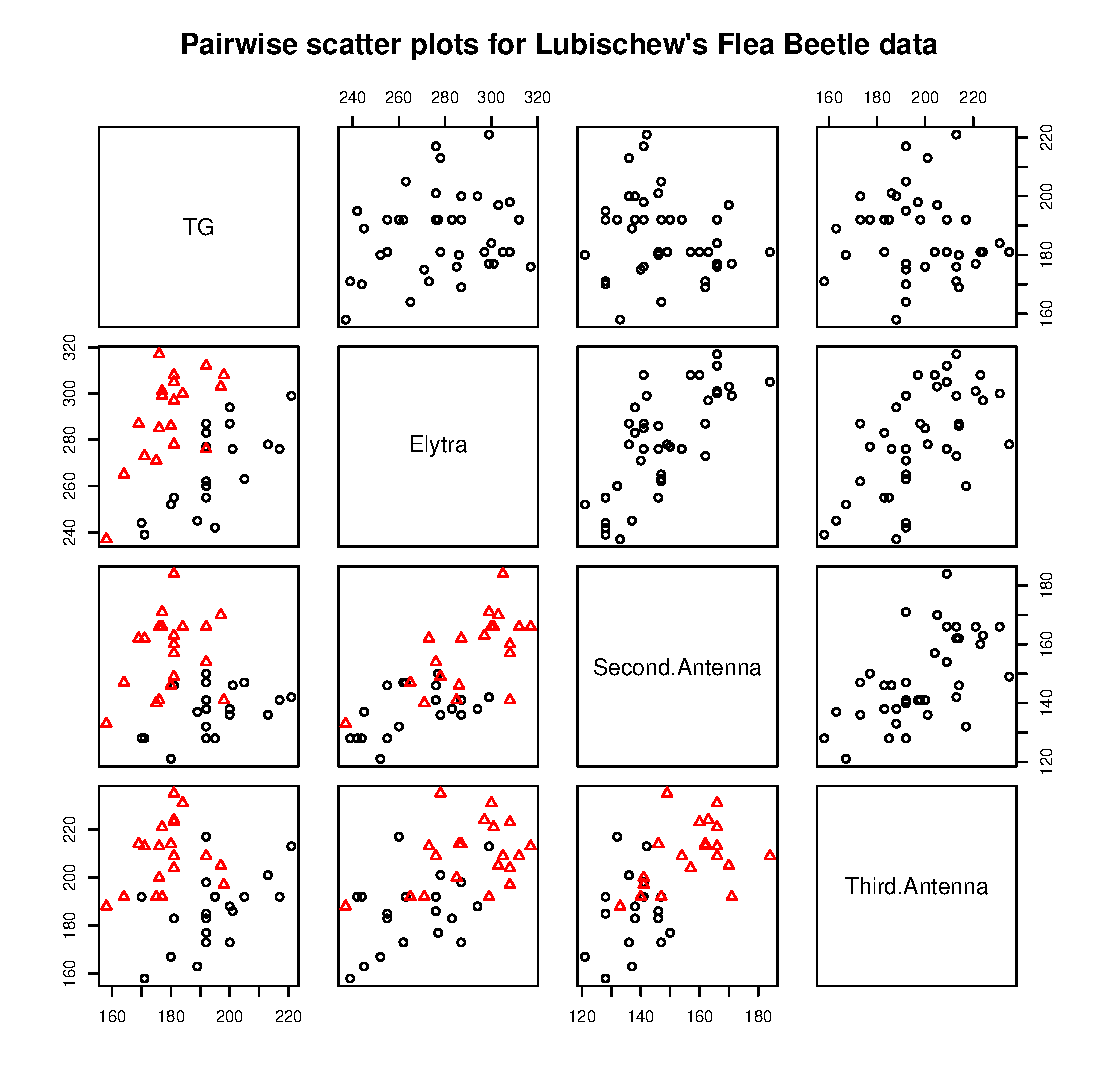
\includegraphics[width = 0.6\textwidth]{images/lubishew}
\caption{Scatterplot for Lubischew flea data, lower panel has symbols denoting the two species}
\label{lubishew}
\end{center}
\end{figure}



\section{Constant Density Ellipses}
\label{cdellipse}

\cite{Flury:1997} gives an interpretation of constant density ellipses in terms of the Mahalanobis distance which is worth reading.   Essentially, we wish to find a region of squared Mahlanobis distance such that:
\begin{displaymath}
Pr \left( (\boldsymbol{\bar{x}} - \boldsymbol{\mu})^{T} \boldsymbol{S}^{-1} (\boldsymbol{\bar{x}} - \boldsymbol{\mu}) \right) c^{2}) 
\end{displaymath}
and we can find $c^{2}$ as follows:
\begin{displaymath}
c^{2} = \left( \frac{n-1}{n} \right) \left( \frac{p}{n-p} \right) F_{(1-\alpha), p, (n-p)}
\end{displaymath}
where $F_{(1-\alpha), p, (n-p)}$ is the $(1-\alpha)$ quantile of the $F$ distribution with $p$ and $n-p$ degrees of freedom, $p$ represents the number of variables and $n$ the sample size.


This illustration is based on, but differs from code provided by Marco Bee to accompany and will make much more sense if used in conjunction with that book.   It is worth checking how and why this code differs!   Firstly, we need a function to draw ellipses:

\singlespacing
\begin{verbatim}
ellipse <- function(covmat, centroid, csquare, resolution, plot = TRUE) {
angles <- seq(0, by = (2 * pi)/resolution, length = resolution)
  sd <- covmat[1,2] / sqrt(covmat[1,1] * covmat[2,2])
    projmat <- matrix(0,2,2)
    projmat[1,1] <- sqrt(covmat[1,1] %*% (1+sd)/2)
    projmat[1,2] <- -sqrt(covmat[1,1] %*% (1-sd)/2)
    projmat[2,1] <- sqrt(covmat[2,2] %*% (1+sd)/2)
    projmat[2,2] <- sqrt(covmat[2,2] %*% (1-sd)/2)
circle <- cbind(cos(angles), sin(angles))
ellipse <- t(centroid + sqrt(csquare) * projmat %*% t(circle))
if (plot == TRUE) {lines(ellipse)}
return(ellipse)
}
\end{verbatim}
\onehalfspacing

It is possible to define a function which calculates $c^{2}$ and calls the ellipse routine (I'm not completely convinced this is doing the calculation correctly yet, in particular I'm not sure I'm using the correct tail).

\singlespacing
\begin{verbatim}
function (data, alpha=0.05, resolution=500) 
{
xbar <- colMeans(data)
n <- dim(data)[1]
p <- dim(data)[2]
f <- qf(1-alpha, p, n-p)
csquare <- ((n-1)/n) * (p / (n-p)) * f
cat(csquare) 
ellipse <- ellipse(cov(data), xbar, csquare, resolution)
}
\end{verbatim}
\onehalfspacing

%# call procedure ellips

%X <- ellips(A, m, const, k)               

%# graph the results

For illustrative purposes, we'll create a $n \times 2$ data object from our flea beetles, and plot the confidence ellipse for these.

\singlespacing
\begin{verbatim}
X <- cbind(flea.beetles[,2], flea.beetles[,3])
plot(X)
cdellipse(X, alpha = 0.01)
cdellipse(X, alpha = 0.05)
\end{verbatim}
\onehalfspacing


These can be contrasted with the univariate confidence intervals:

\singlespacing
\begin{verbatim}
abline(v = confint(lm(X[,1]~1)))
abline(h = confint(lm(X[,2]~1)))
\end{verbatim}
\onehalfspacing

This exercise should be repeated with the turtles data!   However, it is possible to illustrate the basic idea with the sibling heads data, where we construct two derivative variables indicating the difference in head breadth and the difference in head width.   These are plotted in figure \ref{cdellipse}, it can be seen that the univariate confidence intervals and the constant density ellipse support different areas of parameter space.   Ignoring the correlation structure in these data could lead to flaws in inference when assessesing parameter uncertainty.

\begin{figure}
\begin{center}
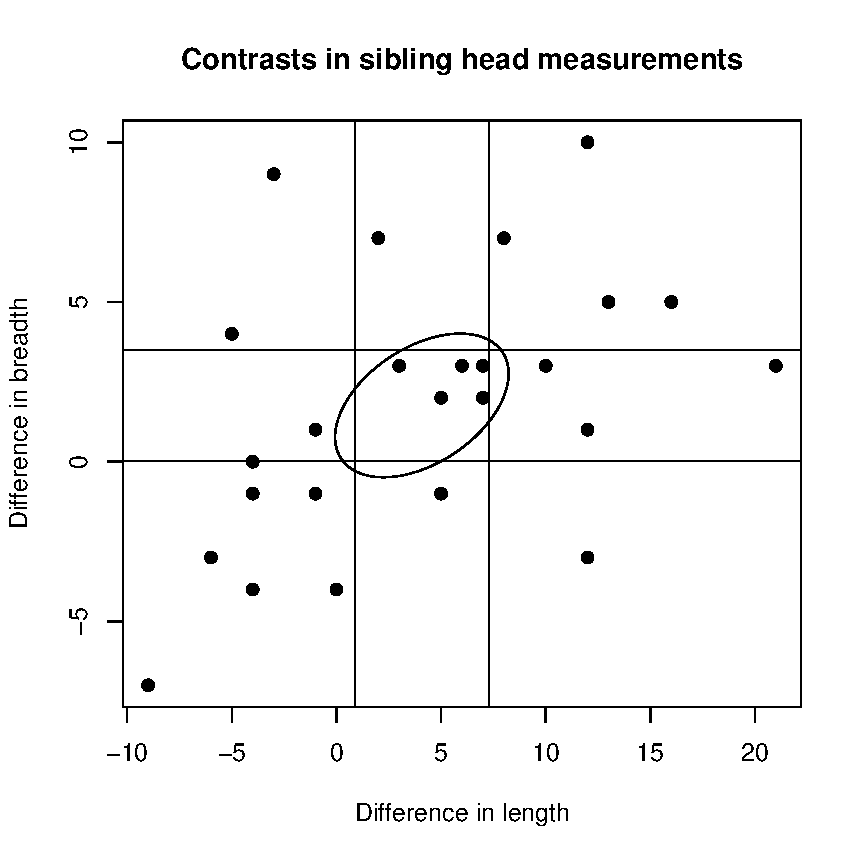
\includegraphics[width = 0.5\textwidth]{images/cdellipse}
\caption{Constant density ellipse for mean vector for difference in head width and breadth, and univariate confidence intervals for the mean of each variable}
\label{cdellipse}
\end{center}
\end{figure}



% X <- sibling.heads
%Y <- cbind((X[, 1] - X[, 3]),(X[, 2] - X[, 4]))
%plot(Y, main = "Contrasts in sibling head measurements", xlab = "Difference in length", ylab = "Difference in breadth", pch = 16)
%X <- Y
%cdellipse(X)
%abline(v = confint(lm(X[,1]~1)))
%abline(h = confint(lm(X[,2]~1)))


%\section{Likelihood ratio tests}
%\label{lrt}

%\section{Profile analysis}
%\label{profile}

%\section{Confidence regions}
%\label{confR}

%\section{Multivariate analysis of variance}
%\label{manova}

%\section{Multivariate regression}
%\label{mvreg}

%\section{Shrinkage of parameters in multivariate regression}
%\label{shrinkage}

%\section{Introduction to the forward search}
%\label{forward}

\section{Multivariate Analysis of Variance}
\label{manova}

As with the univariate situation, t-tests are fine for comparing the means of two groups, but we would have ``multiple comparison'' problems if we tried to compare more than two.   In an analagous way, in the multivariate context we have MANOVA.

First of all we'll enter some data relating to the production of plastic film reported in \cite{Krzanowski:2000}.   Tear, gloss and opacity are measures of the manufactured films.

\singlespacing
\begin{verbatim}
> tear <- c(6.5, 6.2, 5.8, 6.5, 6.5, 6.9, 7.2, 6.9, 6.1, 6.3,                
            6.7, 6.6, 7.2, 7.1, 6.8, 7.1, 7.0, 7.2, 7.5, 7.6)
> gloss <- c(9.5, 9.9, 9.6, 9.6, 9.2, 9.1, 10.0, 9.9, 9.5, 9.4,
             9.1, 9.3, 8.3, 8.4, 8.5, 9.2, 8.8, 9.7, 10.1, 9.2)
> opacity <- c(4.4, 6.4, 3.0, 4.1, 0.8, 5.7, 2.0, 3.9, 1.9, 5.7,
               2.8, 4.1, 3.8, 1.6, 3.4, 8.4, 5.2, 6.9, 2.7, 1.9)
Y <- cbind(tear, gloss, opacity)
\end{verbatim}
\onehalfspacing

We now need to put in information on the rate of extrusion, and the amount of additive used (\texttt{gl()} is a command which specifically creates these kind of experimental factors).

\singlespacing
\begin{verbatim}
> rate <- factor(gl(2,10), labels=c("Low", "High"))
> additive <- factor(gl(2, 5, len=20), labels=c("Low", "High"))
\end{verbatim}
\onehalfspacing

There are three conventional ANOVA that could be considered here, but to consider the three responses together we may wish to conduct a MANOVA.   However, we can use \texttt{manova()} to fit the multivariate ANOVA, and use \texttt{summary.aov()} to extract the results of the unvariate analyses.

There are three matrices of interest in MANOVA:

\begin{itemize}
\item Total SSP ($\boldsymbol{T}$)
\item Between-group SSP ($\boldsymbol{B} = \boldsymbol{T} - \boldsymbol{W}$)
\item Within-group SSP ($\boldsymbol{W}$)
\end{itemize}

Wilk's Lambda is the ratio $\frac{|\boldsymbol{W}|}{|\boldsymbol{T}|}$

\singlespacing
\begin{verbatim}
>      fit <- manova(Y ~ rate * additive)
>      summary.aov(fit)           # univariate ANOVA tables
 Response tear :
              Df  Sum Sq Mean Sq F value   Pr(>F)   
rate           1 1.74050 1.74050 15.7868 0.001092 **
additive       1 0.76050 0.76050  6.8980 0.018330 * 
rate:additive  1 0.00050 0.00050  0.0045 0.947143   
Residuals     16 1.76400 0.11025                    
---
Signif. codes:  0 '***' 0.001 '**' 0.01 '*' 0.05 '.' 0.1 ' ' 1 

 Response gloss :
              Df  Sum Sq Mean Sq F value  Pr(>F)  
rate           1 1.30050 1.30050  7.9178 0.01248 *
additive       1 0.61250 0.61250  3.7291 0.07139 .
rate:additive  1 0.54450 0.54450  3.3151 0.08740 .
Residuals     16 2.62800 0.16425                  
---
Signif. codes:  0 '***' 0.001 '**' 0.01 '*' 0.05 '.' 0.1 ' ' 1 

 Response opacity :
              Df Sum Sq Mean Sq F value Pr(>F)
rate           1  0.421   0.421  0.1036 0.7517
additive       1  4.901   4.901  1.2077 0.2881
rate:additive  1  3.961   3.961  0.9760 0.3379
Residuals     16 64.924   4.058               
\end{verbatim}
\onehalfspacing


A call to \texttt{summary()} will give the MANOVA table.   If you leave out the \texttt{text = \"Wilks\"} call you will get a default Pillai-Bartlett statistic.

\singlespacing
\begin{verbatim}
>      summary(fit, test="Wilks") # ANOVA table of Wilks' lambda
              Df  Wilks approx F num Df den Df   Pr(>F)   
rate           1 0.3819   7.5543      3     14 0.003034 **
additive       1 0.5230   4.2556      3     14 0.024745 * 
rate:additive  1 0.7771   1.3385      3     14 0.301782   
Residuals     16                                          
---
Signif. codes:  0 '***' 0.001 '**' 0.01 '*' 0.05 '.' 0.1 ' ' 1 
\end{verbatim}
\onehalfspacing


As with Hotellings T$^{2}$, Wilk's Lambda has to be converted into an F statistic, a calculation that has been done by the software.   It is possible to approximate this by a $\chi^{2}_{pb df}$ with $W = -\left( w - \frac{p - b + 1}{2}\right)log \Lambda$ where p = number of variables, w = residual degrees of freedom (16), b = number of hypotheses degrees of freedom (1).

In any case, the interaction term is not significant.   We can fit the model without interactions, which as anticipated suggests that both additive and extrusion rate have an effect on the outcome measures.   We will use \texttt{by()} to examine the various group means.

\singlespacing
\begin{verbatim}
> fit <- manova(Y ~ rate + additive)
> summary(fit, test = "Wilks")
          Df  Wilks approx F num Df den Df   Pr(>F)   
rate       1 0.3868   7.9253      3     15 0.002120 **
additive   1 0.5538   4.0279      3     15 0.027533 * 
Residuals 17                                          
---
Signif. codes:  0 '***' 0.001 '**' 0.01 '*' 0.05 '.' 0.1 ' ' 1 
> by(Y, rate, mean) ## group means according to extrusion rate
INDICES: Low
   tear   gloss opacity 
   6.49    9.57    3.79 
------------------------------------------------------------ 
INDICES: High
   tear   gloss opacity 
   7.08    9.06    4.08 
> by(Y, additive, mean) ## group means according to additive
INDICES: Low
   tear   gloss opacity 
   6.59    9.14    3.44 
------------------------------------------------------------ 
INDICES: High
   tear   gloss opacity 
   6.98    9.49    4.43 
> 
> by(Y, list(rate,additive), mean) ## group means by both.
: Low
: Low
   tear   gloss opacity 
   6.30    9.56    3.74 
------------------------------------------------------------ 
: High
: Low
   tear   gloss opacity 
   6.88    8.72    3.14 
------------------------------------------------------------ 
: Low
: High
   tear   gloss opacity 
   6.68    9.58    3.84 
------------------------------------------------------------ 
: High
: High
   tear   gloss opacity 
   7.28    9.40    5.02 
\end{verbatim}
\onehalfspacing

High levels of extrusion rate lead to higher levels of tear and opacity but lower levels of gloss.   High levels of addtive lead to higher levels of tear, gloss and opacity.






%%% Local Variables: ***
%%% mode:latex ***
%%% TeX-master: "../book.tex"  ***
%%% End: ***



%\chapter{Principal Component Analysis}
%    \begin{itemize}
%    \item Properties of eigen decompositions
%    \item Results of principal components (scree plot, loadings, scores, biplots)
%    \item Bootstrapping principal components
%    \end{itemize}


\chapter{Principal component analysis}
\label{pca}


The origins of principal component analysis are usually traced to \cite{Pearson:1901} who was concerned with the fitting planes in the analysis of covariance matrices by orthogonal least squares.   Much development of the technique is ascribed to \cite{Hotelling:1933}, who, working with the correlation matrix provided another development of the technique which is more familiar.    As a technique in its own right it has received book length treatment by \cite{Jackson:1991} and \cite{Jolliffe:1986}; another excellent exposition is given in \cite{Flury:1988} who also develops one generalisation of the technique to multiple groups.   The theory underlying principal components is important in a wide range of areas, consequently this chapter will examine some of the underlying theory as well as considering conventional approaches to principal component analysis.   An \textbf{R}-centric selection of recent extensions to the technique will also be considered in the next chapter.

Principal component analysis can be performed for a variety of reasons, one can perhaps consider its use in one of three ways.   Arguably the most common use is in terms of dimension reduction.   Principal component analysis can be thought of as a data analytic method which provides a specific set of projections\index{projections} which represent a given data set in fewer dimensions.   This has obvious advantages when it is possible to reduce dimensionality to two or three as visualisation becomes very straightforward but it should be acknowledged that reduced dimensionality has advantages beyond visualisation.  Another rationale for conducting principal components analysis is to transform correlated variables into uncorrelated ones, in other words to \emph{sphere} the data.   Whilst univariate data can be standardised by centering and scaling, in a multivariate context one may also wish to ``standardise'' the correlation between variables to zero.    The final rationale for the technique is that it finds linear combinations of data which have relatively large (or relatively small) variability.

In essence, we wish to form projections $\boldsymbol{z} = (z_{1}, z_{2}, \ldots, z_{q})$  of the \emph{standardised} data $\boldsymbol{x} = (x_{1}, x_{2}, \ldots, x_{p})$ 

\begin{eqnarray*}
z_{1} &=& e_{11} x_{1} + e_{12} x_{2} + \ldots e_{1p} x_{p}\\
z_{2} &=& e_{21} x_{1} + e_{22} x_{2} + \ldots e_{2p} x_{p}\\
\ldots\\
z_{q} &=& e_{q1} x_{1} + e_{q2} x_{2} + \ldots e_{qp} x_{p}
\end{eqnarray*}

where the coefficients  $\boldsymbol{E}$ form a $p \times q$ matrix.   If dimension reduction is our goal, clearly we hope that we can form an adequate representation of the data with $q<p$.   

We are going to illustrate Principal Component Analysis by reference to three sets of data.   The first was presented by \cite{Karlis+etal:2003} and relates to Heptathalon results from the Sydney Olympics in 2000.   In this event, athletes compete in seven different sporting activities, and clearly for the purposes of the competition a decision has to be made as to who is the best heptathelete overall.  For sporting purposes, points are awarded for performance in each event and summed.   In essence, a one dimensional composite variable has to be created from the results for the seven events before a decision can be made as to who wins the medals.   We are not necessarily going to challenge the way the International Olympic Committee calculates scores, but clearly a linear combination which achieved maximum separation of athletes might be interesting.   A trivial linear combination would be to take $\boldsymbol{e} = \frac{1}{n}\boldsymbol{1}$.   However, the aim of any projection method is to find an \emph{interesting} projection of the data.   All we need to do is decide what we mean by \emph{interesting}.   As mentioned earlier, one use of principal components is to find projections where the variance is maximised, thus maximising the separation between heptatheletes.  

The second rather well used set of data relates to carapace measurements the painted turtle \textit{Chrysemys picta marginata} first reported by \cite{Jolicoeur+Mosimann:1960}.   These data contain 3 variables recording the shell length, width and height for 24 male and 24 female turtles.   We will consider these data partly because the turtles are cute, but mainly because it affords some consideration of the role of standardisation.   Standardising by subtracting mean and dividing by the standard deviation can be a rather brutal approach, it is possible to take the natural logarithms of these anatomical measures which allows a different insight into the relationship between the measures.

Finally, we will investigate some gene expression data.   In microarray experiments, one typically collects data from a relatively small number of individuals, but records information on gene expression of a large number of genes and therefore have a data matrix $\boldsymbol{X}$ where $n << p$.   Dimension reduction is a central concern at some stage of the analysis, either on the whole set of genes or on a selected subset.   As might become clear, groups of genes which can be identified analytically as co-expressing are referred to as eigengenes.   We will therefore consider some of the issues surrounding the interpretation of principal components in high dimensions.

Some other data sets will be included to illustrate specific points where necessary, and the excercises will also develop other data sets.

%Signature components - linear combinations of the genes that belong to that ocmponent  The first pc is the best 1d representation of a signature component, if genes in a signature component are tightly expressed they will show high correlelation with the pc.  But orthogality, lack of correlation and indepence may be unnecessary requirements. - find loadings and rotate   Simple pca cannot be used with p >> n    -- but we don't want to explain max variance we really want max correlation.


\section{Derivation of Principal Components}

We will firstly consider the derivation of population principal components in the style proposed by \cite{Hotelling:1933} as a way of finding linear combinations with maximum variance.   Given that we have a random vector $\boldsymbol{x} \in \mathbb{R}^{P}$, we wish to consider the vector of transformed variables $\boldsymbol{z} = \boldsymbol{\alpha}^{T}(\boldsymbol{x} - \boldsymbol{\bar{x}})$, and so we wish to find $\alpha$ such that the $\mbox{Var}(z)$ is maximised.  By convention, we insist that $\boldsymbol{\alpha}$ is orthonormal, i.e. in addition to being a vector of unit length we require that $\boldsymbol{\alpha}^{T}\boldsymbol{\alpha} = 1$.   To find an expression for $\mbox{Var}(z)$ in terms of the original variables $\boldsymbol{x}$, firstly by considering the following relationship:
\begin{displaymath}
\mbox{Var}(\boldsymbol{z}) = \mbox{Var}(\boldsymbol{\alpha}^{T}\boldsymbol{x}) = E(\boldsymbol{\alpha}^{T}\boldsymbol{x})^{2}
\end{displaymath}
Hence,
\begin{displaymath}
\sum_{i+1}^{n}(\boldsymbol{z}_{i} - \boldsymbol{\bar{z}})^{2} = \sum_{i=1}^{n}\boldsymbol{\alpha}^{T}\left[(\boldsymbol{x}_{i} - \boldsymbol{\bar{x}})(\boldsymbol{x}_{i} - \boldsymbol{\bar{x}})^{T}\right] \boldsymbol{\alpha}
\end{displaymath}
and premultiplying both sides by $\frac{1}{n-1}$ gives us an estimate of the variance of the transformed variables in terms of the original variables.  To find $\boldsymbol{\alpha}$ in order to maximise the variance we therefore wish to find:  
\begin{equation}
\mbox{max}(\boldsymbol{\alpha}^{T}\boldsymbol{\hat{\Sigma}}\boldsymbol{\alpha})
\end{equation}
subject to the side condition that $\boldsymbol{\alpha}^{T}\boldsymbol{\alpha}= 1$.   Considering the first principal component, we wish to maximise $\mbox{Var}(z_{1}) = \boldsymbol{\alpha}_{1}^{T}\boldsymbol{\hat{\Sigma}}\boldsymbol{\alpha}_{1}$; it can be shown that this problem can be specified by incorporating a Lagrange multiplier.   Consider maximising the expression $\varphi$ given below, where $\lambda$ is a Lagrange multiplier:
\begin{equation}
\varphi_{1} = \boldsymbol{\alpha}_{1}^{T}\boldsymbol{\hat{\Sigma}}\boldsymbol{\alpha}_{1} - \lambda_{1}(\boldsymbol{\alpha}_{1}^{T}\boldsymbol{\alpha}_{1} - 1)
\end{equation}
which can be solved by differentiation with respect to $\boldsymbol{\alpha}_{1}$.   The differential gives us a system of linear equations as follows:
\begin{equation}
\frac{\partial \varphi_{1}}{\partial \boldsymbol{\alpha}_{1}} = 2 \Sigma \boldsymbol{\alpha}_{1} - 2 \lambda \boldsymbol{\alpha}_{1}
\end{equation}
and setting the derivative equal to zero gives:
\begin{equation}
\boldsymbol{\Sigma} \boldsymbol{\alpha}_{1} = \lambda_{1} \boldsymbol{\alpha}_{1}
\end{equation}
which is easily rearranged to give:
\begin{equation}
(\boldsymbol{\Sigma} - \lambda_{1} \boldsymbol{I})\boldsymbol{\alpha} = 0.
\end{equation}

We have $p$ equations and $p$ unknowns, but we can find non-trivial solutions where $\boldsymbol{\alpha} \neq \boldsymbol{0}$ noting that if  $\boldsymbol{a}_{1}^{T}\boldsymbol{a}= 1$ then $\boldsymbol{\Sigma} - \lambda \boldsymbol{I}$ is singular which therefore implies that:
\begin{equation}
|\boldsymbol{\Sigma} - \lambda_{1} \boldsymbol{I}| = 0
\end{equation}

This looks like an eigenproblem, so $\lambda_{1}$ can be found as the largest eigenvalue of $\boldsymbol{\Sigma}$, and $\boldsymbol{\alpha}_{1}$ as the corresponding eigenvector.

For the second principal component, as we are going to assume orthogonality, we wish to add the side condition that $\mbox{Cor}(z_{1},z_{2}) = 0$.   We therefore need to solve:

\begin{equation}
\varphi_{2} = \boldsymbol{\alpha}_{2}^{T}\boldsymbol{\hat{\Sigma}}\boldsymbol{\alpha}_{2} - \lambda_{2}(\boldsymbol{\alpha}_{2}^{T}\boldsymbol{\alpha}_{2} - 1) - \mu(\alpha_{1}^{T}\boldsymbol{\Sigma}\boldsymbol{\alpha_{2}})
\end{equation}
where differentiating now gives:
\begin{equation}
\label{pca2diff}
\frac{\partial \varphi_{2}}{\partial \boldsymbol{\alpha}_{2}} = 2 \Sigma \boldsymbol{\alpha}_{2} - 2 \lambda_{2} \boldsymbol{\alpha}_{2} - \mu \boldsymbol{\Sigma} \boldsymbol{\alpha}_{1}
\end{equation}
but as we assume $\mbox{Cor}(z_{1},z_{2}) = 0$ we take $\boldsymbol{\alpha}_{2}^{T}\boldsymbol{\Sigma}\boldsymbol{\alpha}_{1} = \boldsymbol{\alpha}_{1}^{T}\boldsymbol{\alpha}_{2} = 0$ implying that $\boldsymbol{\alpha}_{1}^{T}\boldsymbol{\alpha}_{2} = \boldsymbol{\alpha}_{2}^{T}\boldsymbol{\alpha}_{1} = 0$ hence we can premultiply our equation in \ref{pca2diff} by $\boldsymbol{\alpha}_{2}$ giving:
\begin{equation}
\label{pca2diff2}
2 \boldsymbol{\alpha}_{2}^{T} \Sigma \boldsymbol{\alpha}_{2} - 2 \boldsymbol{\alpha}_{2}^{T} \lambda_{2} \boldsymbol{\alpha}_{2} - \mu \boldsymbol{\alpha}_{2}^{T} \boldsymbol{\Sigma} \boldsymbol{\alpha}_{1}
\end{equation}
which implies that $\mu=0$, and that $\lambda_{2}$ is also an eigenvalue of $\boldsymbol{\Sigma}$.

Clearly in any formal sense we should continue this process, but the apparent pattern can be demonstrated.   To find further principal components we need to take the spectral decomposition of the covariance matrix, subject to normalising the eigenvectors to have unit length.   In order to find principal components which have maximum variance subject to the condition of being orthogonal to any previous principal component we only need to solve:
\begin{displaymath}
|\boldsymbol{\Sigma} - \lambda \boldsymbol{I}| = 0
\end{displaymath}
and to find:
\begin{displaymath}
\boldsymbol{\Sigma} \boldsymbol{\alpha} = \lambda \boldsymbol{\alpha}
\end{displaymath}

Of some interest to us is that if any matrix $\boldsymbol{\Sigma}$ is symmetric (which will always be the case for correlation and covariance matrices), the normalised eigenvectors corresponding to unequal eigenvalues are orthonormal.

In practice, we don't know $\Sigma$ and we have to estimate it from our data with a suitable estimate.   We can consider a number of possibilities, indeed we will examine robust estimators later.   However, most development of principal components assume the unbiased estimator $\boldsymbol{S} = \frac{1}{n-1} \boldsymbol{X}^{T}\boldsymbol{X}$, where $\boldsymbol{X}$ is a matrix of mean centred data, although we will note later that one of the \textbf{R} functions actually uses $\boldsymbol{S} = \frac{1}{n} \boldsymbol{X}^{T}\boldsymbol{X}$.   $\boldsymbol{\mu}$ is readily estimated from the sample mean.   However, before considering applications to sample principal components, we make a few comments on the geometry of this technique.

\subsection{A little geometry}

Whilst we have covered the variance maximising property of principal components, it is possible to consider the technique from a geometric perspective.   Geometry is perhaps rather more important in recent developments in principal components, details on the concept of \emph{self-consistency} are given by \cite{Flury:1997}. For now, we note that from a geometrical perspective we wish to minimise the perpendicular distance between points and the new projection, the same problem \cite{Pearson:1901} was solving.

Consider the vector of observations $\boldsymbol{x} = (x_{1}, \ldots, x_{p}) \in \mathbb{R}_{p}$   We want to project these obsevations onto $\lambda \boldsymbol{\alpha}$, and in doing so to find the best fitting $q$ dimensional subspace.   Denoting the projection of $\boldsymbol{x}$ by $P\boldsymbol{x}$, we therefore wish to minimise:
\begin{displaymath}
(\boldsymbol{z} - P\boldsymbol{x})^{T}(\boldsymbol{z} - P\boldsymbol{x})
\end{displaymath}

Ideally, we wish the projection to be performed in terms of $\boldsymbol{\alpha} = (\alpha_{1}, \ldots, \alpha_{q})$, although with a $p$ dimensional representation this can clearly take the form $(\alpha_{1}, \ldots, \alpha_{q}, \alpha_{q+1}, \alpha_{p})$.  

The projection can be given as 
\begin{displaymath}
P\boldsymbol{x} = \boldsymbol{x} \boldsymbol{\alpha}^{T}\boldsymbol{\alpha}
\end{displaymath}
where $\boldsymbol{\alpha}^{T}\boldsymbol{\alpha}$ can be described as the projection matrix.   We can rewrite this as:
\begin{displaymath}
P\boldsymbol{x} = \sum_{1}^{q} (x_{i} \boldsymbol{\alpha}_{i}^{T})\boldsymbol{\alpha}_{i}.   
\end{displaymath}
We can therefore rewrite $\boldsymbol{z} - P\boldsymbol{x}$ as 
\begin{displaymath}
\boldsymbol{z} - P\boldsymbol{x} = \sum_{q+1}^{p}(x_{i}^{T} \boldsymbol{\alpha}_{i})\boldsymbol{\alpha}_{i}
\end{displaymath}
Clearly
\begin{displaymath}
(\boldsymbol{z} - P\boldsymbol{x})^{T}(\boldsymbol{z} - P\boldsymbol{x}) = \sum_{q+1}^{p}(x_{i}^{T}\boldsymbol{\alpha}_{i})^{2}
\end{displaymath}

Consequently, we wish to minimise 

\begin{displaymath}
\sum_{j=1}^{p} \sum_{i=1}^{n} (x_{j}^{T}\alpha_{i})^{2}
\end{displaymath}

Which is Pearson's orthogonal least squares problem.  However, we can find a link with Hotelling's approach by noting that $\sum_{j=1}^{n}x_{j}^{T}x_{j} = \sum_{j=1}^{p} \sum_{i=1}^{n} (x_{j}^{T}a_{i})^{2}$ our problem can also be expressed as one where we wish to maximise

\begin{displaymath}
\sum_{j=1}^{p} \sum_{i=1}^{n} (x_{j}^{T}\boldsymbol{\alpha}_{i})^{2}
\end{displaymath}

Noting that this last term is $\sum_{i=1}^{q} \boldsymbol{\alpha}_{i}^{T} \boldsymbol{X}\boldsymbol{X}^{T} \boldsymbol{\alpha}_{i}$, it might be apparent that we actually seek to find $\boldsymbol{\alpha}$, subject to $\boldsymbol{\alpha}^{T}\boldsymbol{\alpha} = \delta$ to maximise $\boldsymbol{\alpha}^{T}\boldsymbol{\Sigma}\boldsymbol{\alpha}$ which looks like a familiar problem!

It may now be noted that the eigenvectors are related to the angle between the untransformed data and the principal component.   Assuming we have $j = 1, \ldots, p$ variables, and $k = 1, \ldots, p$ projections, this angle is given by:
\begin{equation}
\cos \theta_{jk} = \alpha_{jk}
\end{equation}
This is reasonably convenient to plot in 2-dimensions.   Given simulating bivariate data $\boldsymbol{x} = (x_{1}, x_{2})$, the angle between $x_{1}$ and the first principal component is given by $\cos \theta_{11} = \alpha_{11}$.   Rather conveniently, this is implicit in the slope \verb+b=+ supplied to \verb+abline()+.   An illustration of orthogonal projection can be explored using the following code.   This should be contrasted with the least squares fit.

\begin{figure}
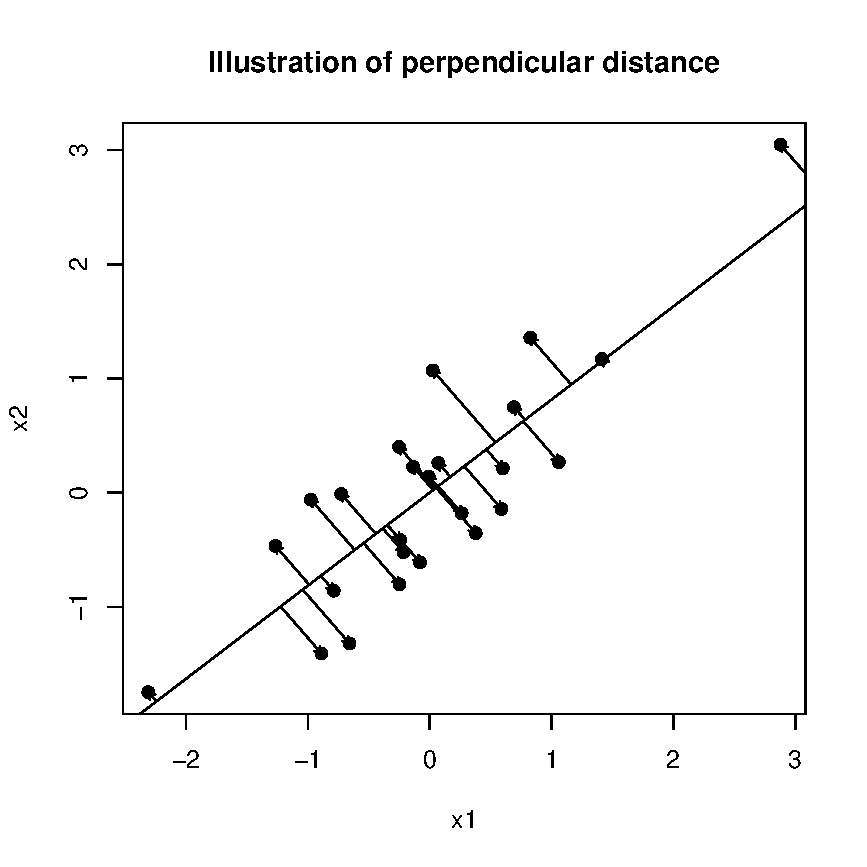
\includegraphics[width = 0.7\textwidth]{images/ProjDist}
\caption{Illustration of perpendicular distance}
\label{projection}
\end{figure}

\singlespacing
\begin{verbatim}
require(MASS)
X <- scale(mvrnorm(25, c(2,2), matrix(c(1,0.8,0.8,1),2,2)))
eqscplot(X)
X.cov <- cov(X)
X.ed <- eigen(X.cov)
proj <- X.ed$vec[,1] %*% t(X.ed$vec[,1])
y <- t(proj %*% t(X))
abline(a=0,b=X.ed$vec[2,1]/X.ed$vec[1,1])
arrows( X[,1], X[,2], y[,1],y[,2], length = 0.05, col = "green")
\end{verbatim}
\onehalfspacing

Plotting the ordinary least squares solutions is easy enough, although when regression X[,1] on X[,2] the gradient needs to be inverted (or the axes reversed).

\singlespacing
\begin{verbatim}
## plot the ols of X[,2] on X[,1]
eqscplot(X)
X2.lm <- lm(X[,2] ~ X[,1])
abline(X2.lm, col = "red", lwd = 2)
arrows(X[,1],X[,2], X[,1], predict(X2.lm),  length = 0.01, col = "red")
points(X[,1],X[,2], pch = 16)
## plot the ols of X[,1] on X[,2]
eqscplot(X)
X1.lm <- lm(X[,1] ~ X[,2])
abline(0, 1/coef(X1.lm)[2], col = "blue")## need to invert the gradient
arrows(X[,1],X[,2], predict(X1.lm), X[,2],  length = 0.01, col = "blue")
points(X[,1],X[,2], pch = 16)
\end{verbatim}
\onehalfspacing


It is informative to contrast the line plotted in figure \ref{projection} with those produced by linear regression of $x$ on $y$ as well as $y$ on $x$.
The matrix $ \boldsymbol{a} \boldsymbol{a}^{T} $ can be referred to as the projection matrix.   

\subsection{Principal Component Stability}
\label{sec:pcastability}

Whilst considering the geometry, it is useful to motivate some ideas about the differences between population and sample principal components by simulating three datasets from the same parameters.   For population 1, we draw from standard normal variables with correlation of 0.9, for population 2 the variables are uncorrelated.   In other words, $\boldsymbol{\mu}_{1} = \boldsymbol{\mu}_{2} = (0,0)^{T}$, $\boldsymbol{\Sigma}_{1} = \left(\begin{array}{rr} 1 & 0.9 \\ 0.9 & 1 \end{array} \right)$ but $\boldsymbol{\Sigma}_{2} = \left(\begin{array}{rr} 1 & 0 \\ 0 & 1 \end{array} \right)$

Simulating the data is simple enough, for example:
\singlespacing
\begin{verbatim}
X <- mvrnorm(100, c(0,0), matrix(c(1,.9,.9,1),2,2))
V <- var(X)
eV <- eigen(V)
\end{verbatim}
\onehalfspacing

\singlespacing
\begin{verbatim}
plot(X, xlim = c(-3,3), ylim = c(-3,3))
abline(a=0,b=eV$vec[2,1]/eV$vec[1,1])
abline(a=0,b=eV$vec[2,2]/eV$vec[1,2])
\end{verbatim}
\onehalfspacing

Just so the eigenvalues don't feel left out, we can add constant density ellipses to these plots, details on these were given in \ref{cdellipse}.  Essentially, we can define a constant density ellipse from the ``centre'' as $\pm c \sqrt{\lambda_{i}} \boldsymbol{\alpha}_{i}$, here we take $c=1.96$.   In the code snippet below, \verb+x+ and \verb+y+ are the coordinates of an ellipse scaled from a unit circle by the two eigenvalues.   These are then rotated by the angles of the eigenvectors:

\singlespacing
\begin{verbatim}
theta <- seq(0,(2*pi),length=101)
x <- 1.96 * sqrt(eV$val[1]) * cos(theta)
y <- 1.96 * sqrt(eV$val[2]) * sin(theta)
newxy <- cbind(x,y) %*% t(eV$vec)
lines(newxy)
\end{verbatim}
\onehalfspacing

We now consider figure \ref{pcastabsynth}, which overlays three samples from each of the two populations specified.   The semi-major axis, the contribution to the first principal component has been denoted with solid lines, the semi-minor axis, the contribution to the second principal component, has been denoted by dotted lines.   It should be very apparent that there is some variation in the orientation of the axes, as might be expected the eigenanalysis varies slightly according to sample properties.   However, the right hand side of the plot is intended to illustrate the problem of sphericity.   Without a strong correlation structure, the angles subtended by the principal components varies massively.

\begin{figure}
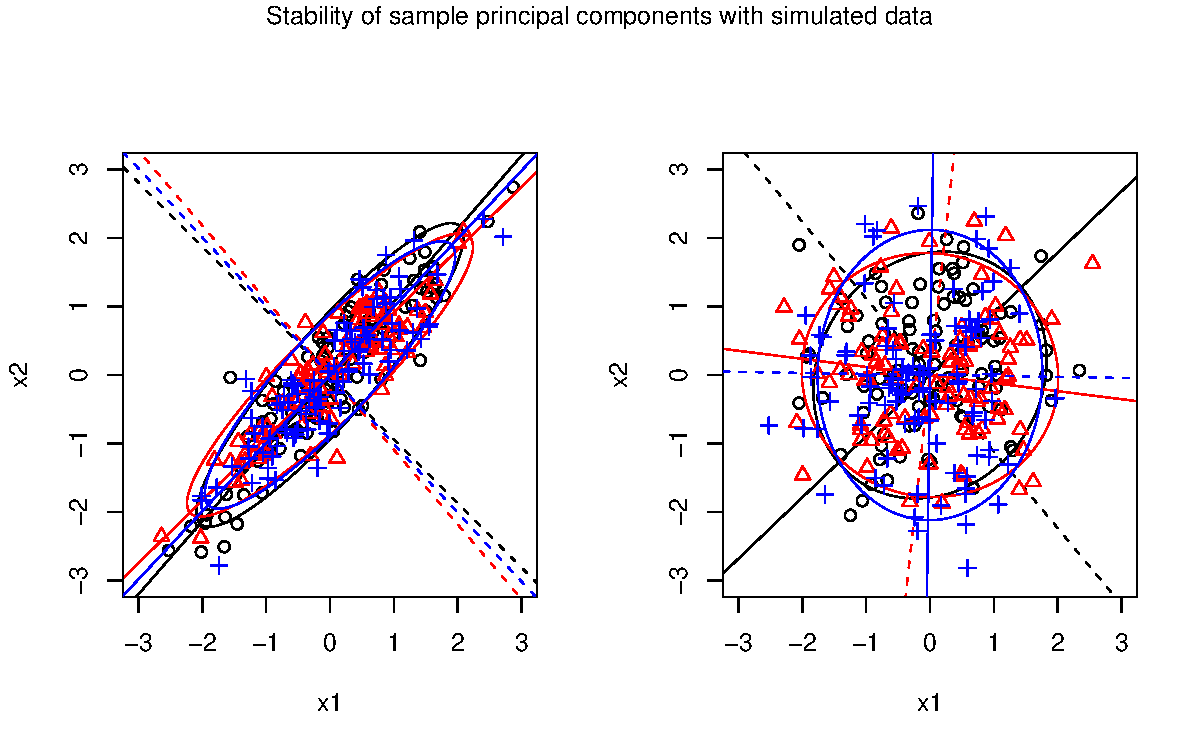
\includegraphics[width = 0.9\textwidth]{images/pcastability}
\caption{Artificially generated data indicating stablity of pca solution}
\label{pcastabsynth}
\end{figure}

Whilst this is an artificial example in many senses (not only are the data simulated but we have only two variables), but the problem is an important one.   In particular, when exploring dimension reduction properties of principal components we have to be attendant to the possibility of partial sphericity; that some of the $q+1, \ldots, p$ principal components essentially exhibit this behaviour.   We consider specific hypothesis tests for this problem later.


Finally, whilst talking about projections, we make one comment in relation to projection pursuit.   This technique will be considered further in the next chapter.   Suffice to say here that projection pursuit is a generic set of techniques which aims to find ``interesting'' projections of data.   The user decides on the dimensionality of the projection and selects a suitable criterion of interestingness.  \cite{Bolton+Krzanowski:1999} give results interpreting principal components analysis within this framework, the criterion (projection pursuit index) in this case is given by:

\begin{displaymath}
I = max(\boldsymbol{e} \boldsymbol{S} \boldsymbol{e}^{T}); \boldsymbol{e}\boldsymbol{e}^{T}=1,
\end{displaymath}
where $\boldsymbol{S}$ is the sample covariance matrix.   This index is the minimum of the maximised log-likelihood over all projections when normality is assumed.

However, they go on to imply that more ``interesting'' projections are less likely to have normally distributed data by showing that in terms of the likelihood$\mathscr{L}(\boldsymbol{e})$, this decreases as $\boldsymbol{e} \boldsymbol{S} \boldsymbol{e}^{T}$ increases.  Assuming the usual maximum likelihood estimators for $\boldsymbol{\mu}$ and $\boldsymbol{\Sigma}$:
\begin{eqnarray*}
\mathscr{L}(\boldsymbol{e}) &=& max \mathscr{L} (\boldsymbol{x}; \boldsymbol{\mu}, \boldsymbol{\Sigma}, \boldsymbol{e})\\
&=& - \frac{n}{2} \left[ p + p \log \left(\frac{2 \pi n}{n-1}\right) \right] - \frac{n}{2} \log |\boldsymbol{e} \boldsymbol{S} \boldsymbol{e}^{T}|
\end{eqnarray*}
In other words, under normality, the most ``interesting'' projection is the one with the maximised likelihood.


\section{Some properties of principal components}

Before considering some examples of principal component analysis we first consider a number of fundamental properties.


\begin{definition}
\label{def:princomp}
If $\boldsymbol{x}$ is a mean centred random vector, with covariance matrix $\boldsymbol{\Sigma}$, the principal components are given by:
\begin{equation}
\boldsymbol{x} \rightarrow \boldsymbol{z} = \boldsymbol{E}^{T}(\boldsymbol{x} - \boldsymbol{\mu})
\end{equation}
i.e. the transformation requires mean-centred variables.   $\boldsymbol{E}$ is orthogonal, $\boldsymbol{E}^{T}\boldsymbol{\Sigma}\boldsymbol{E}$ is diagonal, $\lambda_{1} \geq \lambda_{2} \geq \ldots \geq \lambda_{p} \geq 0$ provided $\boldsymbol{\Sigma}$ is positive definite.
\end{definition}

A number of key propeties immediately follow from their derivation from the spectral decomposition:


\begin{theorem}
\begin{equation} 
\label{pcszero}
\mbox{E}(z_{i}) = 0
\end{equation}

\begin{equation}
\mbox{Var}(z_{i}) = \lambda_{i}
\end{equation}
hence:
\begin{equation}
\mbox{Var}(z_{1}) \geq \mbox{Var}(z_{2}) \geq \ldots \geq \mbox{Var}(z_{p});
\end{equation}
in particular it should be noted that no standardised linear combination of $\boldsymbol{x}$ has a larger variance than $\boldsymbol{\lambda}$.

We finally restate the implications of finding orthogonal projections.
\begin{equation}
\mbox{Cov}(z_{i},z_{j}) = 0, i \neq j;
\end{equation}

\end{theorem}


One property we will make repeated use of concerns the proportion of variance explained by each principal component:

\begin{theorem}
\label{th:eigentrace}
The trace of a covariance matrix is equal to the sum of its eigenvalues:
\begin{equation}
\label{eigentrace}
trace(\boldsymbol{\Sigma}) = \sum_{i=1}^{p} \lambda_{i}
\end{equation}
\end{theorem}

In other words, equation~\ref{eigentrace} indicates that the \emph{total variance} can be explained by the sum of the eigenvalues.   In the case of principal components formed from the correlation matrix $\boldsymbol{R}$ this will be equal to the number of variables.


\begin{theorem}
\label{th:eigenproduct}
The generalised variance (the determinant of a covariance matrix) can be expressed as the product of its eigenvalues:
\begin{equation}
\lvert \boldsymbol{\Sigma} \rvert = \prod_{i = 1}^{p} \lambda_{i}
\end{equation}
\end{theorem}
Theorem \ref{th:eigenproduct} indicates that we can find an estimate of the \emph{generalised variance} from the product of the eigenvalues.   Along with theorem \ref{th:eigentrace} we find that the generalised variance and the sum of variances are unchanged by the principal component transformation.   

Finally, a note is needed on scale-invariance.   \cite{Flury:1997} describes this last as an anti-property.   Principal components are not-invariant to changes of scale.   Standardising variables is rather a brutal way of dealing with this.   Explanations are given in most multivariate textbooks, for example both formal and information explanaitions are given by [page 219] \cite{Mardia+etal:1979}.   Nevertheless, if variables are recorded on widely differing scales, a principal component analysis of the covariance matrix will largely reflect the variables with the numerically greatest variance.   It is therefore important that the variables are in some sense comparable; this can either be achieved by standardising, or by some gentler transformation.   We will find that the heptathalon data has to be standardised, whereas it is possible to take logs of the turtle data.


Finally, we consider one important property, which is more in the \cite{Pearson:1901} sense.   

\begin{theorem}
The first $k$ principal components have smaller mean squared departure from the population (or sample) variables than any other $k$-dimensional subspace.
\end{theorem}
Proof: [page 220] \cite{Mardia+etal:1979}

This property is rather important when considering the dimension reducing properties of principal component as it does not require any distributional assumptions.



\section{Illustration of Principal Components}

 We define the sample principal components by $\boldsymbol{e}$ and $\ell$.

Having now hopefully explained the rationale behind principal components analysis, we consider some illustrative analysis before considering further inferential developments.

\subsection{An illustration with the Sydney Heptatholon data}

Before doing anything else with these data, it needs to be noted that in the three running events, better performance is indicated by a lower measure (time), whereas in the jumping and throwing events good performance is indicated by a higher measure (distance).   It seems sensible to introduce a scale reversal so that good performance is in some way at the top of any given scale.   A convenient way of doing this is to multiply the times of the running events by $-1$.

\singlespacing
\begin{verbatim}
hept.df <- read.csv("Heptatholon.csv", row.names = 1)
hept.df$X100mHurdles.S. <- hept.df$X100mHurdles.S. * -1
hept.df$X200m.sec. <- hept.df$X200m.sec. * -1
hept.df$r800m.s. <- hept.df$r800m.s. * -1
\end{verbatim}
\onehalfspacing

These variables are clearly incomparably in any sense.    It is also clear that we need to work with the correlation matrix for these data, there is considerable difference in the scales (running 800 metres tends to take rather longer than running 100 metres).   We will also centre the variables using \verb+scale()+ which saves us a little work later on.  

\singlespacing
\begin{verbatim}
hep.scale <- scale(hept.df[,-1])
hept.cormat <- cor(hept.df[,-1])
hep.ev <- eigen(hept.cormat)
\end{verbatim}
\onehalfspacing

Our principal component analysis then basically consists of extracting \verb+hep.ev$values+ contains the eigenvalues, and \verb+hep.ev$vectors+ contains the eigen vectors.   Our first set of loadings are given by the first row of the eigenvectors, we can form the first linear combination:

\singlespacing
\begin{verbatim}
> hep.ev$vectors[,1]
> z1 <- hep.scale %*% hep.ev$vectors[,1]
\end{verbatim}
\onehalfspacing

in a similar manner it is possible to form $z_{2}$ and so on.  


This means that the proportion of total variance explained by each linear combination can be given by $\frac{\lambda_{i}}{ \sum_{i=1}^{p} \lambda_{i}}$
, which can be calculated for our heptathalon data with \verb+hep.ev$values/sum(hep.ev$values)+.   It is also conventional to produce a ``scree'' plot of this information with something like \verb+plot(hep.ev$values, type = "b")+ which graphically represents the amount of variance explained by each linear combination.

%par(las = 1)
%plot(hep.ev$values, type = "b", main = "Scree plot from Heptathalon data", ylab = "Variance explained", xlab = "Principal component", pch = 16)


\begin{figure}
\begin{center}
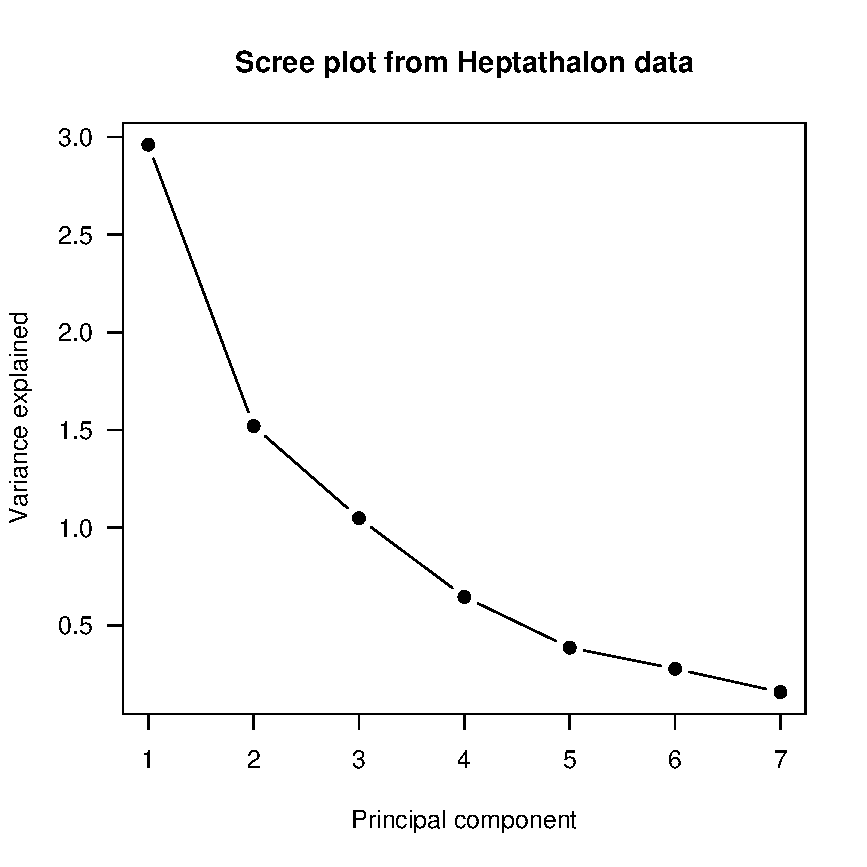
\includegraphics[width = 0.5\textwidth]{images/HeptathScree} 
\caption{Scree plot displaying the amount of variation explained by each of the seven principal components formed from the correlation matrix of the Sydney Heptathalon data}
\label{screeplot}
\end{center}
\end{figure}


\subsection{Principal component scoring}

As stated at the start of the chapter, the principal component scores are essentially derived from the mean centered data.   

In other words, we found:

\begin{equation}
\label{pcascore}
\boldsymbol{z} =  \boldsymbol{E}^{T}(\boldsymbol{x}-\boldsymbol{\mu})
\end{equation}

It is possible (although somewhat unusual in this context) to find scores from the standardised data

\begin{equation}
\boldsymbol{z} =  \boldsymbol{E}^{T}(\boldsymbol{x}-\boldsymbol{\mu})  \boldsymbol{\Lambda}^{-1/2}
\end{equation}

It should be noted that \cite{Rencher:2002} really doesn't approve of this latter effort, it essentially leaves us looking at the correlation between the standardised data and the principal component scores.   We therefore consisder the more usual scores given in equation \ref{pcascore}.   The first four eigenvectors are given as follows:

\singlespacing
\begin{verbatim}
$vectors
           [,1]        [,2]        [,3]         [,4]
[1,] -0.4656494  0.28868133  0.32883275 -0.003922038  
[2,] -0.2455859 -0.56442826 -0.10737271 -0.610427608  
[3,] -0.4195748 -0.07137064 -0.52173345  0.235891780 
[4,] -0.4330174 -0.02204083  0.51825157  0.357022268 
[5,] -0.4630436  0.11516723  0.12459693 -0.480637087 
[6,] -0.3228125  0.38161226 -0.56832241  0.091073036 
[7,] -0.2017272 -0.65849286 -0.03216966  0.452710298 
\end{verbatim}
\onehalfspacing

So to find the first principal component we only need to compute the following:

\begin{displaymath}
z_{i1} = a_{11} x_{i1} + a_{12} x_{i2} + a_{13} x_{i3} + \ldots
\end{displaymath}

which means that the first principal component can be given as:

\begin{displaymath}
Z_{i1} = -0.4656 \times x_{1} - 0.2456 \times x_{2} - 0.4196 \times x_{3} + \ldots
\end{displaymath}

Clearly this can also be calculated as matrix product $\boldsymbol{X}\boldsymbol{a}$.

\singlespacing
\begin{verbatim}
hep.ev$vectors[,1] ## first vector of pc loadings
scores <- hep.scale %*% hep.ev$vectors
par(mfrow = c(3,3))
apply(scores, 2, qqnorm)
scoresR <- hep.scale %*% (hep.ev$vectors %*% diag(hep.ev$values^-0.5))
\end{verbatim}
\onehalfspacing

If we wished, we can carry out further investigation of the principal component scores.


\subsection{Prepackaged PCA function 1: \texttt{princomp()}}

In practice it will come as no surprise to learn that there are prepackaged functions in \textbf{R} for carrying out a principal components analysis.   \verb+princomp()+ has been provided for comparability with S-Plus.  We will find out later that the preferred function uses the singular value decomposition.   However, there are good reasons for examining \verb+princomp()+ first.    It is based on carrying out an eigen decomposition, by default of the covariance matrix and it should be noted that the covariance matrix esimated by \verb+cov.wt+ uses the divisor $N$, rather than the unbiased version $N-1$.    It is possible to supply robust estimates of the covariance matrix via \verb+covmat+, this does allow a form of robust principal components and as we work through the heptathalon data we will find out that this may indeed be useful.  
It is possible to call \verb+princomp()+   with the specification \verb+cor=TRUE+ to use the sample correlation matrix rather than sample covariance matrix.

The main results can be accessed via \verb+summary()+ and \verb+print()+.   The eigenvectors are extracted and printed with a degree of pretty printing using \verb+loadings()+.   If necessary, the square roots of the eigenvalues (i.e. the standard deviations of each principal component) are stored within the princomp object and can be extracted manually using \verb+$sdev+.   The principal component scores themselves can be accessed via \verb+$scores+ if these have been requested.    There are also graphical methods associated with \verb+princomp()+ objects, \verb+plot()+ produces a screeplot, \verb+biplot()+ produces a biplot, we explain this tool further in section~\ref{prcomp}.   However, we note an important aspect of eigenanalysis, which is very clearly stated in the helpfile and will be quite important later:
\begin{quote}
The signs of the columns of the loadings and scores are arbitrary, and so may differ between different programs for PCA, and even  between different builds of R.
\end{quote}
This is a point we will return to a few times particularly when considering bootstrapping!

Executing a principal component analysis is therefore trivial, as demonstrated in the following code snippet.   We extract the principal component scores and create qq plots; as demonstrated in chapter 2 any univariate linear combination of multivariate normal data should be normally distributed.  

\singlespacing
\begin{verbatim}
hept.princomp <- princomp(hept.df[,-1], scale = TRUE)
summary(hept.princomp)
plot(hept.princomp) ## produces scree plot
par(mfrow = c(3,3))
apply(hept.princomp$scores, 2, qqnorm)
\end{verbatim}
\onehalfspacing


\subsection{Inbuilt functions 2: \texttt{prcomp()}}
\label{prcomp}

The preferred \textbf{R} function for a conventional principal component analysis is \verb+prcomp()+.   There are a number of differences in use and extraction, but the rather more important difference is that it is based upon a singular value decomposition of the data.   The singular value decomposition was outlined in Section~\ref{svd}.   Whilst discussing the singular value decomposition in this context it is convenient to introduce the biplot.   \cite{Gabriel:1971} introduced the biplot as a means of representing either a matrix of rank two, or a rank two approximation to a matrix of rank greater than two.   The idea is to display vectors for each row and vectors for each column are displayed on the same plot, illustrating features of either a rank two matrix or a rank two approximation.   Whilst we illustrate it in detail here, it has application in areas other than with principal components.

As discussed earlier, we consider data matrix $\boldsymbol{X}$; it's decomposition is given by:
\begin{displaymath}
\boldsymbol{X} = \sum_{i=1}^{p} \lambda_{i} \boldsymbol{u}_{i} \boldsymbol{v}_{i}^{T}
\end{displaymath}
and hence for the biplot, where we specifically require a rank two solution:
\begin{displaymath}
\boldsymbol{X} = \sum_{i=1}^{2} \lambda_{i} \boldsymbol{u}_{i} \boldsymbol{v}_{i}^{T} = 
\left( \boldsymbol{u}_{1},  \boldsymbol{u}_{2} \right) 
\left( \begin{array}{cc} \lambda_{1} & 0 \\ 0 & \lambda_{2} \end{array} \right) \left( \begin{array}{c} \boldsymbol{v}_{1}^{T} \boldsymbol{v}_{2}^{T} \end{array} \right)
\end{displaymath}

Based on this decomposition, we have a choice of plots.   In general, we can plot:
\begin{displaymath}
\boldsymbol{g}_{i}^{T} = \lambda_{1}^{1-\zeta} u_{1i}, \lambda_{1}^{1-\zeta} u_{2i}
\end{displaymath}
for the observations
and
\begin{displaymath}
\boldsymbol{h}^{T}_{j} = \lambda_{1}^{\zeta} q_{1j} \lambda_{2}^{\zeta} q_{2j}
\end{displaymath}
for the columns.
where $0 \leq \zeta \leq 1$.   \cite{Gabriel:1971} essentially gave proposals for $\zeta = 0$, $\zeta = 0.5$ and $\zeta = 1$.   In \textbf{R}, these can be set with the argument \verb+scale+ which takes the range $0 \leq \mbox{scale} \leq 1$.   The default is \verb+scale = 1+ which implies $\boldsymbol{H}^{T}\boldsymbol{H} = \boldsymbol{I}$; more notably this means that the inner products between variables approximate covariances and distances between observations approximate Mahalanobis distance.    By default, observations are scaled up by $\sqrt{n}$, variables are scaled down by $\sqrt{n}$

It is possible to adjust \verb+choices=c(1,2)+ if you don't really want a biplot but want to examine the projection of what are in this context other principal components.


\singlespacing
\begin{verbatim}
pairs(turtles[,-1],
   lower.panel = function(x, y){ points(x, y,
   pch = unclass(turtles[,1]),
   col = as.numeric(turtles[,1]))},
   main = "Pairwise scatter plots for painted turtles")
\end{verbatim}
\onehalfspacing

We follow \cite{Flury:1997} in transforming these data onto the log scale (and multiplying them by 10).   This is quite common in allometric applications, where the $\log$ transformation may suffice in terms of bringing all variables onto a comparable scale.

\singlespacing
\begin{verbatim}
data(turtles)
  turtles.m <- subset(turtles, turtles$Gender == "Male")
  turtles.m <- 10 * log(turtles.m[,-1])
  turtles.m.prcomp <- prcomp(turtles.m)
  summary(turtles.m.prcomp)
plot(turtles.m.prcomp)
turtles.m.prcomp$sdev^2 ## extract eigenvalues
par(xpd = NA)
biplot(turtles.m.prcomp)
\end{verbatim}
\onehalfspacing

%turtles.prcomp <- prcomp(turtles[,-1])
%plot(turtles.prcomp$x[,1], turtles.prcomp$x[,2],
% col = as.numeric(turtles[,1]),
% pch = as.numeric(turtles[,1]))

We can illustrate the biplot as follows by carrying out the various computations by hand within \textbf{R}:

\singlespacing
\begin{verbatim}
turtles.svd <- svd(turtles.m)
H <- cbind(turtles.svd$u[,1], turtles.svd$u[,2]) * sqrt(24)
g1 <- turtles.svd$d[1] * turtles.svd$v[,1] / sqrt(24)
g2 <- turtles.svd$d[2] * turtles.svd$v[,2] / sqrt(24)
plot(H)
par(new = TRUE)
plot(c(-arrx,arrx),c(-arry,arry), type = "n",
  xaxt = "n", yaxt = "n")
axis(3)
axis(4)
arrows(0, 0, arrx, arry)
\end{verbatim}
\onehalfspacing


\section{Principal Components Regression}

Finally, we say a few words about principal components regression, and illustrate the use of principal components in bioinformatics with the superpc package.


\section{``Model'' criticism for principal components analysis}

This section has deliberately given a provocative title.   ``Model'' criticism clearly requires some kind of model, it is worth giving some thought to whether we are using a principal components model in the context of a model or not.   It is possible to use the technique as a data analytical technique, particularly when used for data reduction there is no necessity to assume multivariate normality.   However, when we are using it in the context of a multivariate normal distribution, it is important to be aware of a number of key distributional results on the asymptotic distribution of the eigenvalues and eigenvectors of a covariance matrix.


\subsection{Distribution theory for the Eigenvalues and Eigenvectors of a covariance matrix}

\cite{Girshink:1939,Anderson:1963} give results for asymptotic distributions in connection with the covariance matrix.   Firstly, we comment on the existence of maximum likelihood estimators for the eigendecomposition of a covariance matrix:

\begin{theorem}
\label{th:evalmle}
Under conditions of normality, the maximum likelihood estimators for the population eigenvalues and eigenvectors of $\boldsymbol{\Sigma}$ are given by the sample eigenvalues and eigenvectors, provided all the eigenvalues are distinct.
\end{theorem}
Proof: See [page 229] \cite{Mardia+etal:1979} and [page 460] \cite{Anderson:1984}



Theorem \label{th:evalmle} indicates that our sample eigenvalues are the maximum likelihood estimators of their corresponding population counterparts.   In most inferential situations we would wish to qualify such an estimator with guidance as to the level of associated uncertainty.   Firstly, we wish to establish the distribution of the eigenvalues.

\begin{theorem}
\label{th:pcasymptotics}
The asymptotic distribution of eigenvalues and eigenvectors can be expressed as follows:
\begin{equation}
\label{pcasymptotics}
\sqrt{n}(\boldsymbol{\ell} - \boldsymbol{\lambda}) \sim MVN(\boldsymbol{0}, 2\boldsymbol{\Lambda}^{2})
\end{equation}
%\begin{equation}
%\sqrt{n} \frac{\mathscr{l}_{i} - \lambda_{i}}{\sqrt{2}\mathscr{l}_{i}} \to^\infty N(0,1)
%\end{equation}
where $\Lambda$ is the diagonal matrix of eigenvalues.   This can be expressed equivalently as:
\begin{equation}
\label{pcaasymptoticslog}
\sqrt{n}\left(\log(\boldsymbol{\ell}) - \log(\boldsymbol{\lambda})\right) \sim MVN(\boldsymbol{0}, 2)
\end{equation}

 and 
\begin{equation}
\sqrt{n}(\hat{\boldsymbol{e}}_{i} - \boldsymbol{e}_{i}) \sim MVN(\boldsymbol{0}, \boldsymbol{E}_{i})
\end{equation}
where $\boldsymbol{E}_{i} = \lambda_{i} \sum_{k = 1, k \neq i}^{p} \frac{\lambda_{k}}{(\lambda_{k} - \lambda_{i})^{2}} \boldsymbol{e}_{k}\boldsymbol{e}^{T}$
\end{theorem}
Proof: The proof for this has been restated in \cite{Flury:1988}.   These properties were established following work by \cite{Anderson:1963} and \cite{Girshink:1939}.


Theorem \ref{pcasymptotics} indicates that for large $n$, the eigenvalues $\lambda_{i}$ are independently distributed.   We can therefore obtain standard errors for the eigenvalues as follows:
%\subsection{Confidence intervals for the eigenvalues and eigenvectors}
%\label{pcaconfint}
\begin{displaymath}
se(\lambda_{j}) = \sqrt{2/n} \lambda_{j},
\end{displaymath}
giving confidence intervals:
\begin{displaymath}
\frac{\ell_{i}}{1 + \sqrt{2/n} z_{\alpha/2}} \leq \lambda_{i} \leq \frac{\ell_{i}}{1 + \sqrt{2/n} z_{1-\alpha/2}}
\end{displaymath}
and the standard error for the corresponding eigenvectors are given by: 
\begin{displaymath}
se(\alpha) = \left( \frac{1}{n} \lambda_{j} \sum_{j+1; j \neq h}^{p} \frac{\lambda_{j}}{(\lambda_{j} - \lambda_{h})^2} \alpha_{jh}^{2} \right)^{1/2}.
\end{displaymath}


We can illustrate calculation of these standard errors, as well as estimation of associated confidence intervals by adapting code written by Marco Bee  to accompany \cite{Flury:1997}).   This code will be set out at an S3 class in \textbf{R}.   Firstly therefore, we set out a container:
\singlespacing
\begin{verbatim}
lpc <- function(X){
  UseMethod("lpc", X)
}
\end{verbatim}
\onehalfspacing

And now we can write out a default method which calculates the relevant confidence intervals:
\singlespacing
\begin{verbatim}
lpc.default <- function(X)
{
n <- dim(X)[1]; p <- dim(X)[2]  # number of observations 
X.prcomp <- prcomp(X)
evals <- X.prcomp$sdev^2 
Ones <- matrix(1, p, p) 
Lambda <- Ones * evals
Q <- (t(Lambda) - Lambda + diag(p))^(-2) - diag(p) # nifty trick
Theta1 <- sweep(Q, 2, evals, FUN="*") 
Theta <- Theta1 * evals # compute matrix of theta-coefficients
stdeB <- matrix(0,p,p)      
   h <- 1
      while (h <= p){ 
      V <- X.prcomp$rotation %*% 
          (Theta[, h] * t(X.prcomp$rotation))  
      stdeB[, h] <- sqrt(diag(V)/n)
      h <- h + 1 
      }                         
stdelam <- sqrt(2/n) * evals
results <- list("eigenvectors" = X.prcomp$rotation, 
  "eigenvalues" = X.prcomp$sdev^2,
  "stdeB" = stdeB, "stdelam" = stdelam)
  class(results) <- "lpc"
  results
}
\end{verbatim}
\onehalfspacing

Having returned the standard error we can write a simpler print function which displays the eigenvectors and eigenvalues along with their associated standard error:
\onehalfspacing
\begin{verbatim}
print.lpc <- function(x) {
print(x[1]) ## eigenvectors
print(x[2]) ## eigenvalues
cat("standard errors for eigenvector coefficients:")
print(x[3])
cat("standard errors for eigenvalues:")
print(x[4])
cat("\n\n")
invisible(x)
}
\end{verbatim}
\onehalfspacing

So for example, with the turtles data:
\singlespacing
\begin{verbatim}
> lpc(subset(turtles, turtles$Gender == "Male")[,-1])
$eigenvectors
          [,1]        [,2]        [,3]
[1,] 0.8401219  0.48810477 -0.23653541
[2,] 0.4919082 -0.86938426 -0.04687583
[3,] 0.2285205  0.07697229  0.97049145

$eigenvalues
[1] 195.274633   3.688564   1.103833

standard errors for eigenvector coefficients:$stdeB
           [,1]       [,2]       [,3]
[1,] 0.01442666 0.04469703 0.07885419
[2,] 0.02487011 0.01592627 0.13874655
[3,] 0.01513963 0.15478836 0.01276277

standard errors for eigenvalues:$stdelam
[1] 56.370931  1.064797  0.318649

\end{verbatim}
\onehalfspacing

And if we wanted to estimate the confidence intervals we can write an associated \verb+summary+ method which will do the additional calculations and return the results.   Note in the code below that we have allowed for a \emph{Bonferroni} adjustment.   If we wish to adjust for making $m$ comparisons we can replace $z_{\frac{\alpha}{2}}$ with $z_{\frac{\alpha}{2m}}$  

\singlespacing
\begin{verbatim}
summary.lpc <- function(x, alpha = 0.05, bonferroni = FALSE) {
if (!is.null(alpha)){ ## calculate ci if asked
  if (bonferroni == TRUE) {alpha = alpha / length(x[[2]])}
  z <- abs(qnorm((1-alpha)/2))
}
print(x[1]) ## eigenvectors

if (!is.null(alpha)){
cat(round(alpha * 100), "\% CI: \n ")
veclo <- x[[1]] - z * x[[3]]
vechi <- x[[1]] + z * x[[3]]
print(veclo)
print(vechi)
cat("\n")
} 

print(x[2]) ## eigenvalues

if (!is.null(alpha)){
cat(round(alpha * 100), "\% CI: \n ")
vallo <- x[[2]] - z * x[[4]]
valhi <- x[[2]] + z * x[[4]]
print(vallo)
print(valhi)
cat("\n")
} 

cat("standard errors for eigenvector coefficients:")
print(x[3])

cat("standard errors for eigenvalues:")
print(x[4])
cat("\n\n")
invisible(x)
}
\end{verbatim}
\onehalfspacing

%This should place some cautions on arbitrary cutoffs, e.g. Kaiser.


\section{Sphericity}
\label{Sphericity}

We preface this section on sphericity with some results concerning covariance / correlation matrices which are of less than full rank.   If a symmetric positive definite matrix (correlation and covariance matrices are at least semi-definite).   If such a matrix is of full rank $p$ then all the eigen values are positive.   
%If the matrix is of rank $m < p$ then there will be $m$ positive eigenvalues and $p-m$ zero eigenvalues.   We will consider this sphericity problem in some detail later.
%We preface comments on sphericity with one point concerning the rank of the covariance or correlation matrix.   
If the rank of the covariance or correlation matrix $m < p$ then the last $p-m$ eigenvalues are identically zero.   The converse of this theorem is that any non-zero eigen value can be considered to be \emph{significantly} non-zero.

However, we are now going to consider sphericity, where there are not $p$ distinct eigenvalues.   We highlighted earlier the potential problem of sphericity and the effect on a resultant principal component analysis.
Clearly there is little point carrying out a principal component analysis under conditions of sphericity.   We can consider three possiblilites, where $\boldsymbol{R} = \boldsymbol{I}$, which can arise either because $\boldsymbol{S} = s \boldsymbol{I}$ or the more general possibility that $\boldsymbol{S}$ is diagonal.


We firstly consider the most general possibility, that $\boldsymbol{\Sigma} \propto \sigma \boldsymbol{I}$ where $\sigma$ is unspecified.   However, this test is equivalent to examining whether all the roots of $|\boldsymbol{\Sigma} - \lambda \boldsymbol{I}| = 0$ are equal.   In this eventuality, the arithmetic and geometric means will be identical

We firstly consider a general test for sphericity proposed by \cite{Mauchly:1940}


\begin{theorem}
We consider that:
\label{th:sphericity}
\begin{displaymath}
\frac{\prod_{j=1}^{p} \lambda_{i}^{1/j}}{\sum_{j=1}^{p} \lambda_{i}^{1/j}} = \frac{\lvert \boldsymbol{\Sigma} \rvert^{1/j}}{\frac{1}{j} tr(\boldsymbol{\Sigma})}
\end{displaymath}

This yields the following test statistic.   Under the null hypothesis $H_{0}: \boldsymbol{S} = \sigma \boldsymbol{I}$, the test statistic $m$ given by:
\begin{equation}
m = \frac{\lvert \boldsymbol{S} \boldsymbol{\Sigma}_{0}^{-1} \rvert^{n/2}}
{ \left[ \frac{1}{p} trace(\boldsymbol{S} \boldsymbol{\Sigma}_{0}^{-1} )^{pn/2} \right] } 
\end{equation}
\end{theorem}


This is pre-implemented in \textbf{R} for manova type objects, therefore if we fit a null manova object we can carry out this test:

\singlespacing
\begin{verbatim}
obj <- manova(as.matrix(turtles.m) ~ 1)
mauchly.test(obj)

        Mauchly's test of sphericity

data:  SSD matrix from manova(as.matrix(turtles.m) ~ 1) 
= 101.1821, p-value < 2.2e-16
\end{verbatim}
\onehalfspacing

And so we have evidence (provided the test assumptions are met) that the turtle data are not spherical.


For completeness, we mention here another test for sphericity is given by [see section 1.9] \cite{Morrison:2005} based upon the determinant of the correlation matrix.

\begin{definition}
\label{morrison}
Under the null hypothesis $H_{0}: \boldsymbol{R} = \boldsymbol{I}$, the test statistic $w$ given by:
\begin{displaymath}
w = -\left( n - \frac{2p + 5}{6} \right) \log \lvert \boldsymbol{R} \rvert
\end{displaymath}
has a $\chi^{2}$ distribution with $\frac{1}{2}p(p-1)$ degrees of freedom.
\end{definition}

This test is quite simply coded up in \textbf{R}.

\singlespacing
\begin{verbatim}
morrison <- function(data){
  n <- dim(data)[1]; p <- dim(data)[2];
  wnm <- -(n - (2 * p)/6) * log(det(cor(data)))
    cat(paste("wnm = ", wnm, "\n"))
    cat(paste("df = ", p * (p - 1) * 0.5, "\n"))
    cat(paste("Chisq density = ", dchisq(wnm, p * (p - 1) * 0.5) , "\n"))
}
\end{verbatim}
\onehalfspacing

Again, this test confirms non-sphericity of the Turtles data.

\subsection{Partial sphericity}

It is usually the case that partial sphericity is or more practical concern than more complete independence of the data.   We will consider more heuristic methods for selecting the dimensionality of a principal component projection later, but clearly the eigenvectors of principal components with equal eigenvalues are too poorly defined to be of any practical use.   We are therefore interested in partial sphericity, where $\lambda_{q+1} = \lambda_{q+2} = \ldots = \lambda_{p}$

%We highlighted in theorem \ref{pca:lowrank} that whenever the covaraiance matrix had rank $r<p$ there were $r$ principal components.   More notably, we highlighted the problem in \label{sec:pcastability} of sphericity.   In practice, we may be more concerned about partial sphericity; whilst the first $q$ eigenvalues are distinct we may be concerned that the smallest eigenvalues, $q+1, \ldots, p$, are equal.   

Where we have partial sphericity, we may note the following theorem:

\begin{theorem}
For normal data, where the eigenvalues of $\boldsymbol{\Sigma}$ are not distinct then the m.l.e. of $\bar{\lambda}$ is the corresponding arithmetic mean of the sample eigenvalues, and the corresponding eigenvectors are maximum likelihood estimators although they are not unique.
\end{theorem}
Proof: See \cite{Anderson:1963}

The asymptotic theory set out above leads to a number of possible tests for partial sphericity.   One likelihood ratio can be considered as follows:

\begin{definition}

[page 198] \cite{Seber:1984} gives a likelihood ratio test for partial sphericity.   In order to determine whether whether the last $p-q$ eigenvalues are equal can be specified as follows.   We wish to test $H_{0}: \lambda_{q+1} = \lambda_{q+2} = \ldots = \lambda_{p}$ versus $H_{a}: \lambda_{q+1} > \lambda_{q+2} > \ldots > \lambda_{p}$.

\begin{equation}
-2 \log \mathscr{l} = - n \log \left( \prod_{q=1}^{p} \frac{\lambda_{j}}{\bar{\lambda}} \right)
\end{equation}
where $\bar{lambda} = \frac{1}{p-q} \sum_{j=q}^{p} \lambda_{j}$.   Under the null hypothesis, the likelihood ratio statistic, $-2 \log \mathscr{l}$, of the eivenvalues derived from a covariance matrix is distributed as $\chi^{2}_{\frac{1}{2}(p-q-1)(p-q+2)}$.  The test can be applied to the correlation matrix but the asymptotic distribution is no longer chi-square.   The asymptotics can be improved with a correction proposed by \cite{Lawley:1956}:

%this uses Anderson:1963 and Fujikoshi:1978 asymptotics on chisq.

\begin{equation}
- \left\{ n - 1 - q - \frac{2(p-q)^{2} + (p-q) + 2}{6(p-q)} + \sum_{j=1}^{q} \left(\frac{\bar{\lambda}}{\lambda_{j} - \bar{\lambda}} \right)^2 \right\}  \log \left( \prod_{q=1}^{p} \frac{\lambda_{j}}{\bar{\lambda}} \right)
\end{equation}

This test is however not robust to departures from normality.


%\label{th:sphertest}
%The likelihood ratio test for the hypothesis $\lambda_{q+1} = \cdots = \lambda_{p}$ versus the alternative $\lambda_{q+1} > \cdots \lambda_{p}$ is given by:

%\begin{equation}
%\varphi(q, p-q) = N(p-q) 
%\frac{\frac{1}{p-q} \sum_{j=q=1}^{p} \lambda_{j}}
%{(\prod_{j=q=1}^{p} \lambda_{j} )^{1/(p-q)}}
%\end{equation}
%\end{theorem}
%Proof: \cite{Anderson:1984}

%$\varphi \sim \chi_{((p-q)((p-q)+1)/2 - 1)}^{2} as N \rightarrow \inf$

%It is therefore possible to test for sphericity of a $q$ dimensional solution, increasing this by one and not worrying about the multiple testing problem.

\end{definition}

It is reasonably straightforward to start coding a function to execute this in \textbf{R}, a sketch of such a function is illustrated here:
\singlespacing
\begin{verbatim}
spher <- function(X, q){
  p <- dim(X)[2]; n <- dim(X)[1]; r <- p-q
  X.prcomp <- prcomp(X)
  evals <- X.prcomp$sdev^2
  retain <- evals[1:q]; discard <- evals[-(1:q)]
  lambdahat <- mean(discard)
  bit <- sum(lambdahat / (retain - lambdahat) )^2
  corr <- n - 1 - q - (2 * r^2 + r + 2)/(6*r) + bit
  product <- prod(discard / lambdahat)
  lrt <- -corr * log(product)
  df <- 0.5 * (r-1) * (r+2)
    cat(paste("-2log L = ", lrt, "\n") )
    cat(paste("df = ", df, "\n") )
    cat(paste("Chisq density ", dchisq(lrt, df ), "\n" ))
    ##return(lrt)
}
\end{verbatim}
\onehalfspacing

We illustrate this with the turtle data.   Recalling that the first eigenvalue was 2.33, considerably greater than the second and third eigenvalues of 0.06 and 0.036.

\singlespacing
\begin{verbatim}
> spher(turtles.m, 1)
-2log L =  1.34290454195737 
df =  2 
Chisq density  0.255482988814162 
\end{verbatim}
\onehalfspacing

So in this case we cannot reject $H_{0}$ and have no evidence that the second and third eigenvalues are distinct.   We might be included to consider the possibility here that that $\lambda_{2} = \lambda_{3}$ and would therefore be somewhat wary of the resultant eigenvectors.


A simpler explanation is given in [page 622] \cite{Flury:1997}, which follows from that given in [page 475] \cite{Anderson:1984}, and is given in slightly different form in [page 235] \cite{Mardia+etal:1979}.%##mkb <- n* p * (a - 1 - log(g) ) ##mkb pg 235
This relies on a log likelihood statistic derived as a ratio of arithmetic to geometric means of the eigenvalues.

\singlespacing
\begin{verbatim}
function(X, q){
  p <- dim(X)[2];  n <- dim(X)[1];  r <- p-q
  X.prcomp <- prcomp(X)
  evals <- X.prcomp$sdev^2
  q1 <- q+1
    discard <- evals[q1:p]
    a <- sum(discard) / r
    g <- prod(discard)^(1/r)
    s <- n * r * log(a / g)
    df <- 0.5 * r * (r+1)
  cat(paste("-log L = ", s, "\n") )
  cat(paste("df = ", df, "\n") )
  cat(paste("Chisq density ", dchisq(lrt, df ), "\n" ))
  ##return(s)
}
\end{verbatim}
\onehalfspacing

Asymptotically, this value can be considered to follow a $\chi^{2}_{\frac{1}{2}(p-q)(p-q+1) - 2}$ distribution under the null hypothesis.   It can be seen that is related to the test of complete sphericity.   This test can be used with the turtle data and again confirms the possible that the second and third principal components can be considered spherical and should not be interepreted further.


%Yet another likelihood ratio test exists for this.

%\begin{displaymath}
%\Lambda = \frac{|\boldsymbol{S}|^{n/2}}{\prod s_{ij}^{n/2}} = |\boldsymbol{R}|^{n/2} < c
%\end{displaymath}
%$-2 \log \Lambda \sim \chi^{2}$ with Bartlett continuity corrections

%In the case of the latter, $\lambda = 1 + (p-1) \rho$, eigenvectors = $\frac{1}{\sqrt{p}}$


\subsection{High Dimensional Tests for Sphericity}

Having (hopefully) demonstrated the importance of sphericity in conventional principal components analysis we refer to results which carry out analagous procedures in high dimensions.   Whilst the asymptotic tests above rely on $n \to \infty$, it can be problematic where $p > n$.   More recent work therefore examines how one might carry out tests for this eventually.   We firstly consider testing whether $\boldsymbol{\Sigma} \propto \boldsymbol{I}$ 

\begin{theorem}
A test for $\boldsymbol{\Sigma} \propto \boldsymbol{I}$ which is reliable whenever $p > n$ can be given as follows:
\begin{equation}
U = \frac{1}{p} trace \left( (\frac{\boldsymbol{S}}{(1/p)trace(\boldsymbol{S})} - \boldsymbol{I} )^{2} \right)
\end{equation}
In this case, it may be noted that $\frac{np}{2} U$ asymptotically follows a $\chi^{2}$ distribution with $\frac{1}{2}p(p+1)-1$ degrees of freedom. 

Proof: See \cite{Ledoit+Wolf:2002}, following work by \cite{John:1971,John:1972}
\end{theorem}

This can be very simply estimated in \textbf{R}:

\singlespacing
\begin{verbatim}
JohnsU <- function(data){
  p <- dim(data)[2]
  S <- cov(data)
  traceS <- sum(diag(S))
  traceSI <- sum(diag(S-diag(rep(1, p))))
    u <- 1/p * traceS / (1/p*traceSI^2)
    test <- n * p * 0.5 * u
    df <- (0.5 * p * (p+1)) - 1
  cat(paste("U = ", test, "\n") )
  cat(paste("df = ", df, "\n") )
  cat(paste("Chisq density ", dchisq(test, df ), "\n" ))
}
\end{verbatim}
\onehalfspacing

So we can estimate the sphericity quite simply

\singlespacing
\begin{verbatim}
JohnsU(khan$train)
\end{verbatim}
\onehalfspacing

Which appears to indicate little evidence for sphericity.

Testing the correlation matrix is not quite so straighforward to expansion of $p$ relative to $n$.    $\boldsymbol{\Sigma} = \boldsymbol{I}$

\begin{theorem}
A test for $\boldsymbol{\Sigma} = \boldsymbol{I}$ which is reliable whenever $p > n$ is given by:
\begin{equation}
\label{ledoit}
W = \frac{1}{p} trace \left\{ \left( \boldsymbol{S} - \boldsymbol{I} \right)^{2} \right\} - \frac{p}{n} \left\{ \frac{1}{p} trace(\boldsymbol{S}) \right\}^{2} + \frac{p}{n}
\end{equation}
Under $H_{0}$, assuming multivariate normality $\frac{nm}{2} W \rightarrow ^{d} \chi^{2}_{p(p+1)/2-1}$

Proof: \cite{Ledoit+Wolf:2002}
\end{theorem}

\singlespacing
\begin{verbatim}
ledoitwolf <- function(data){
  n <- dim(data)[1]; p <- dim(data)[2] 
  S <- cor(data)
  traceS <- sum(diag(S))
  SI <- crossprod(S - diag(rep(1, p)))   
  traceSI <- sum(diag(SI))
    w <- 1/p*traceSI - p/n*(1/p*traceS)^2 + p/n
    test <- n * p * 0.5 * w
    df <- (0.5 * p * (p+1))
  cat(paste("U = ", test, "\n") )
  cat(paste("df = ", df, "\n") )
  cat(paste("Chisq density ", dchisq(test, df ), "\n" ))
}
\end{verbatim}
\onehalfspacing


However, we can consider results based on those indicated in  \ref{morrison} which can be used to test whether $\boldsymbol{R} = \boldsymbol{I}$.  

\begin{theorem}
A test statistic for sphericity is given by:
\begin{displaymath}
t = \sum_{i=2}^{p} \sum_{j=1}^{i-1} r_{ij}^{2} - \frac{p(p-1)}{2n}
\end{displaymath}
Which is asymptotically normal with zero mean and variance:
\begin{displaymath}
\sigma_{t}^{2} = \frac{p(p-1)(n-1)}{n^{2}(n+2)}
\end{displaymath}
Proof: See \cite{Schott:2005}
\end{theorem}


This is simply illustrated in \textbf{R}.

\singlespacing
\begin{verbatim}
schott <- function(data){
  n <- dim(data)[1]; p <- dim(data)[2]
  R <- cor(data)
  R[lower.tri(R) == FALSE] <- NA
  red <- na.omit(as.vector(R))
   tnm <- sum(red^2) 
   cf <- (p * (p-1)) / (2 * n)
   test <- tnm - cf
   sigma2 <- (p * (p-1) * (n-1)) / (n^2 * (n+2) )
  cat(paste("tnm = ", tnm, "cf = ", cf,  "\n") )
  cat(paste("Normal density ", dnorm(test, sqrt(sigma2) ), "\n" ))
}
\end{verbatim}
\onehalfspacing

Again, a call to \verb+schott(khan$train)+ confirms that these data are non-spherical.

As before, perhaps we are more interested in the generalisations of these statistics, i.e. we are concerned with partial sphericity and wish to determine whether the smallest $p-q$ eigenvalues of $\boldsymbol{\Sigma}$ are equal.

\begin{theorem}
Generalising equation \ref{ledoit}, a test for partial sphericity can be based upon the following test statistic:
\begin{equation}
u = \frac{ (1/p) \sum_{i=q+1}^{p} \lambda_{i}}{\left[(1/p) \sum_{i=q+1}^{p} \lambda_{i} \right]^{2}} - 1
\end{equation}
where $\frac{n-q}{u}$\footnote{check this} can be compared with a $\chi^{2}$ distribution with $p(p+1)/2 - 1$ degrees of freedom.     
\end{theorem}
Proof: \cite{Schott:2006}

Again, this test can be coded up in \textbf{R} and examined in the context of the khan data.

\singlespacing
\begin{verbatim}
schottpartial <- function(X, q){
  p <- dim(X)[2]; n <- dim(X)[1]; r <- p-q
  X.prcomp <- prcomp(X)
  evals <- X.prcomp$sdev^2
  discard <- evals[-(1:q)]
  u <- (sum(discard^2) / r) / (sum(discard) / r)^2  - 1
  df <- 0.5 * r * (r+1) - 1
    cat(paste("u = ", u, "\n") )
    cat(paste("df = ", df, "\n") )
    cat(paste("Chisq density ", dchisq(u * (n-q), df ), "\n" ))
    ##return(lrt)
}
\end{verbatim}
\onehalfspacing




It is bearing in mind that just because the smallest $p-q$ eigenvalues indicate the corresponding principal components explain very little of the variation, they do not necessarily contain any useful information.


%library(made4)
%data(khan)
%khan.coa<-ord(khan$train, classvec=khan$train.classes, type="pca")  
%khan.coa$ord$eig
%dim(khan$train)


%\begin{displaymath}
%U_{r} \left( \frac{
%\frac{1}{r}  sum_{i+q+1}^{p} \lambda_{i}^{2} }
%{(\frac{1}{r} sum_{i+q+1}^{p} \lambda)^{2}} - 1 \right)
%\end{displaymath}
%where $r = p-q$, i.e. we are looking for a test to reject the $r$th smallest eigenvalues.   It can be shown that testing $(n-q) U_{r} > \chi^{2}_{\frac{r(r+1)}{2}-1, 1-\alpha}$, where $\alpha$ is the required significance level and 



\section{How many components to retain}

We have considered formal hypothesis testing for sphericity and partial sphericity.   This may well indicate that it is not sensible to include a number of principal components in a given representation of multivariate data.   However, we may not really be interested in modelling multivariate normality.   We may not like asymptotics.   We will consider a few further results on selecting the number of principal components in any given projection of the data.

Whilst principal components have optimality properties in terms of providing the best lower dimensional projection in terms of mean squared error.   Nevertheless, they are often used, however informally, in an inferential role.   Consideble care is needed in their interpretation.   It is important to note that we are working with sample principal components, these can be somewhat unstable relative to the puted underlying population components.   It makes little sense to attempt anything resembling inferential work without considering the stability of a particular principal component solution.   Typically, having decided how best to scale the data, the next most important question surrounds how many components need to be retained.   We will first consider some of the more informal procedures used to guide this judgement, and will subsequently consider methods derived from normal theory inference.



\subsection{Data analytic diagnostics}

A number of proposals have been made in the literature concerning decisions surrounding the ``number of components'' to retain.  The following are some of the more popular proposals:

%\begin{itemize}
%\item Retaining enough components to explain more than x\% of the variation, where x has been determined \textit{a priori} and is in the order of 80 or 90\%.
%\item Looking for a change in the slope of the scree plot - the last components where the line flattens are usually discarded
%\item Interpreting the scree plot in the presence of monte carlo simulations
%\item Retaining all components explaining an above average amount of variation (i.e. in the case of components derived from the correlation matrix this is all components with an eigenvalue above 1)
%\item Broken stick approach
%\item Using the empirical distribution function, i.e. bootstrapping
%\end{itemize}


\subsection{Proportion of variance explained}
\label{propexpl}

The proportion of variance explained is a rather informal method for selecting $q$, the number of dimensions in the principal component projection required to adequately explain the data.   Essentially, one decides \textit{a priori} that a certain amount of variance is to be explained, and only accepts solutions meeting that requirement.   It is however consistent with the exploratory nature to which principal component analysis is often applied.


We can however, using the asymptotic theory set out above, develop a confidence interval for the proportion of variance explained.   %We suggested in section \ref{propexpl} that one might choose the dimensionality of the solution based on whether it meets some predetermined arbitrary proportion of variance.  We have confidence intervals for these values as well.

\begin{theorem}
\label{th:propexpl}

We denote our estimate of the proportion of variation explained by $\pi$:
\begin{displaymath}
\pi = f(\lambda) = \frac{ \sum_{i=1}^{q} \lambda_{i} }{ \sum_{i=1}^{p} \lambda_{i} }.
\end{displaymath}

If we also consider the corresponding sum of squares:
\begin{displaymath}
\zeta = \frac{\sum_{i=1}^{q} \lambda_{i}^{2}}{ \sum_{i=1}^{p} \lambda_{i}^{2}}
\end{displaymath}

Under conditions of multivariate normality, we can obtain an estimate of the variance associated $\pi$, the proportion of variance explained as follows:
\begin{equation}
\eta^{2} = \frac{2 trace(\Sigma)}{(n-1)  (trace(\Sigma))^{2}} = \pi^{2} - 2 \zeta \pi + \zeta^{2}
\end{equation}
\end{theorem}
\textbf{Proof}: \cite{Sugiyama+Tong:1976} and [page 454] \cite{Kshinaragar:1972}

Hence we can derive a confidence interval for $\pi$ as follows.

This can be illustrated as follows:

\singlespacing
\begin{verbatim}
vals <-  hep.ev$values^2
q <- 3
alpha <- 0.95
alpha <- 1 - (1-alpha)/2

pi <- sum(vals[1:q]) / sum(vals)
alpha <- sum(vals[1:q]^2) / sum(vals^2)## by vector recycing
eta2 <- pi^{2} - 2 * alpha * pi + alpha^2
cat(pi, eta2)
cat("\n")
cat(pi + qnorm(alpha)*eta2)
cat("\n")
cat(pi - qnorm(alpha) * eta2)
cat("\n")
\end{verbatim}
\onehalfspacing





\subsection{Change in slope of the scree plot}
\label{screeslope}

\cite{Cattell:1966} proposed the scree plot in the context of (principal component extracted) factor analysis.   Without wishing to add to the confusion between the two techniques, it has become a fairly standard technique for assessing the adequacy of a number of dimension reducing techniques.   Both \texttt{prcomp} and \texttt{princomp} objects have a plot method which yields a scree plot, the idea is to select components up to the point where the slope changes direction.

\singlespacing
\begin{verbatim}
plot(hept.princomp)
\end{verbatim}
\onehalfspacing

\subsection{Interpreting the scree plot in the presence of simulations}
\label{screemc}

It is possible to extend the basic scree plot idea.   \cite{Horn:1965} suggested simulating data from a multivariate normal having the same sample size, the same number of variables, the same means and variances but having zero covariances.   There are a couple of manifestations of this approach within various \textbf{R} packages, for example \verb+psy+ package contains a ready made function.   The scree plot of with zero correlation is expected to be a straight line, it can be compared with the scree plot from the observed data.   It is possible to extend this to a full Monte Carlo test, the code listing below goes someway towards this.

\singlespacing
\begin{verbatim}
Horn <- function(data, reps){
p <- dim(data)[2]
n <- dim(data)[1]
Varmat <- matrix(0,p,p)
Mean <- mean(data)
diag(Varmat) <- diag(var(data))

Evals <- princomp(data, cor = TRUE)$sdev^2
idx <- barplot(Evals, names.arg = paste("PC", c(1:7)), 
xlab = "Component", ylab = "Proportion of trace", 
main = "Proportion of trace explained")

results <- matrix(0,reps,p)
  for (i in 1:reps){
  SimData <- mvrnorm(n, Mean, Varmat)
  ExpEvalsH <- princomp(SimData, cor = TRUE)$sdev^2
  results[i,] <- ExpEvalsH
  lines(idx, ExpEvalsH, type = "b", pch = 16)
  }

lines(idx, apply(results, 2, mean), type = "b", col = "red")

legend("topright", lty = 1, pch = 16, legend = "Expected values")
Results <- data.frame(Evals = Evals, ExpEvalsH = ExpEvalsH)
}

Horn(hept.df[-1], 10)
\end{verbatim}
\onehalfspacing

\includegraphics[width = 0.7\textwidth]{images/Horn}


\subsection{Broken Stick}
\label{brokenstick}

Another approach to assessing the proportion of variation explained has been made by \cite{Jolliffe:1986} who suggests using a ``broken stick'' approach.   The idea here is that if any unit is randomly divided into $p$ segments, the expected length of the $k$th longest segment is:
\begin{equation}
\label{stick}
l_{k} = \left(\frac{1}{p} \right) \sum_{i=k}^{p} \left( \frac{1}{i} \right)
\end{equation}
If we assume that the total variance, $trace{\boldsymbol{S}} = \sum_{j=1}^{p}$, is the ``stick'', we can use this approach to estimate an expected size of each eigenvalue.   A rather simple function to calculate the expected values indicated by \ref{stick} is given below, the expected values are plotted alongside the observed values from a \texttt{princomp()} object created from the Heptathalon data.   It should be noted that \texttt{princomp()} returns the standard deviations (\verb+$sdev+), these have therefore been squared to recoved the eigenvalues $\lambda_{i}$.

\singlespacing
\begin{verbatim}
> stickometer <- function(p){
  vec <- 1 / (1:p)
  stick <- vector("numeric", p) 
  stick[1] <- sum(vec)
     for (i in 2:p){
     stick[i] <- sum(vec[-(1:(i-1))])}
  stick <- 1/p * stick
  names(stick) <- paste("Comp.", c(1:p), sep = "")
  return(stick)
}
> 
> stick <- stickometer(7)
> proptrace <- hep.princomp$sdev^2 / sum(hep.princomp$sdev^2)
>
> stick
> proptrace
> 
> idx <- barplot(proptrace, names.arg = paste("PC", c(1:7)), 
> xlab = "Component", ylab = "Proportion of trace", 
> main = "Proportion of trace explained")
> lines(idx, stick, type = "b", pch = 16)
> legend("topright", lty = 1, pch = 16, legend = "Expected values")
\end{verbatim}
\onehalfspacing

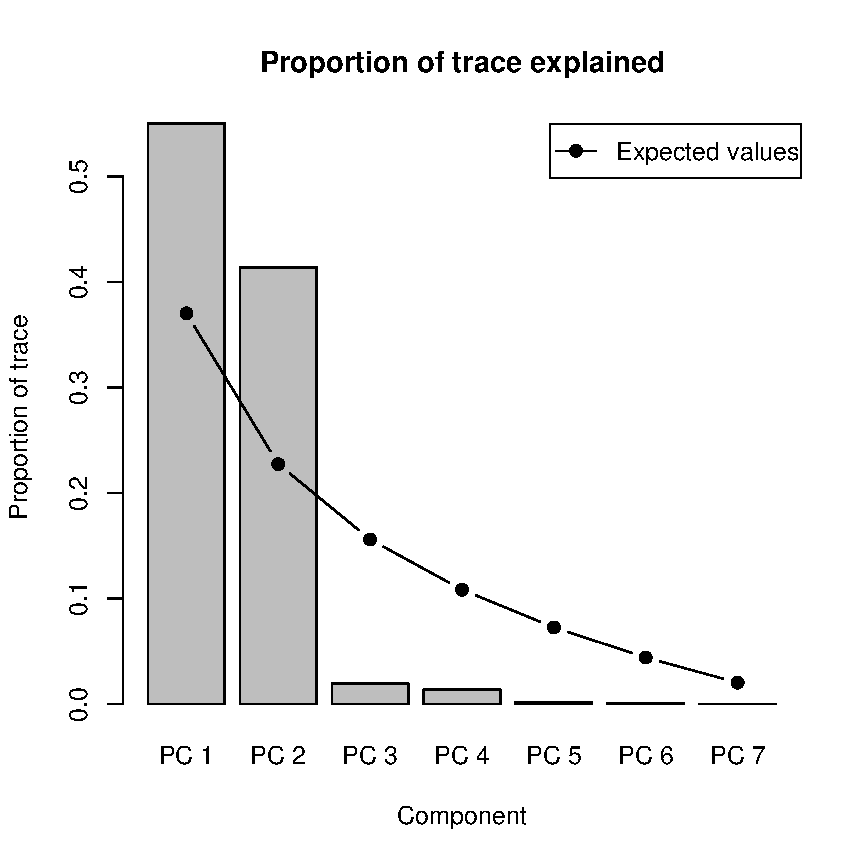
\includegraphics[width = 0.7\textwidth]{images/stick}

Examination of the results (numbers or the plot) suggest that the first and seventh components are accounting for slightly more variation than would be expected purely by chance.

\subsection{Kaiser Criterion}
\label{kaiser}

The Kaiser Criteria is a rather inflexible criteria widely met in many sofware packages.   Basically it amounts to retaining all components where the eigenvalue is greater than the mean of the eigenvalues.   In the case of principal components based on the correlation matrix this clearly means retaining all components where the eigenvalue is greater than one.  Whilst one may not wish to assume multivariate normality, the asymptotics considered next provide a clear warning that population eigenvalues greater than one could clearly be realised in a sample with values below one.


Karlis provide some caveats on the use of this criteriosn.

\subsection{Cross validation}

Cross-validation in the context of principal components was proposed by \cite{Wold:1976,Wold:1978} and developed by \cite{Eastment+Krzanowski:1982}.   In essence, the sample can be randomly split into $g$ groups, the loadings can be estimated from reduced sets omitting each of the $g$ groups in turn, but the predicted values can be found from these $g$ groups using the loadings estimated from the other rows.   The value for $(\boldsymbol{\hat{x}} - \boldsymbol{x})$ can be estimated from equation \ref{Qstats}, and the PRESS statistic estimated.


\singlespacing
\begin{verbatim}
pcaxv <- function(X){
  UseMethod("pcaxv", X)
}
\end{verbatim}
\onehalfspacing

It is useful to create an \texttt{S3} object to carry out this procedure.   The working function is given by:

\singlespacing
\begin{verbatim}
pcaxv.default <- function(X, g = 5){
    N <- dim(X)[1]
    p <- dim(X)[2]
      index <- sample(c(1:N) )
      groups <- gl(g, N %/% g)
         Q <- matrix(0, g, p)
           for (i in 1:g){
           dot <- prcomp(X[-index[groups == i],])
         Q[i,] <- colSums((as.matrix(scale(X))[index[groups == i],]
                       %*% dot$rotation)^2)}
    colmeans <- colSums(Q) / N
  PRESS <- cumsum(colmeans[c(p:1)])/ c(1:p)
  PRESS <- PRESS[c(p:1)]
  names(PRESS) <- paste("C", c(0:(p-1)))
  results <- list("PRESS" = PRESS, 
    dm = pcaxvconstants(N,p)$dm, dr = pcaxvconstants(N,p)$dr)
class(results) <- "pcaxv"
results
}
\end{verbatim}
\onehalfspacing

The function \verb+pcaxvconstants()+ calculates some constants that can be used in the summary function.   A suitable print function for use with cross-validation objects created here can be given as follows:

\singlespacing
\begin{verbatim}
print.pcaxv <- function(x){
cat("Components Removed \n")
  print(x[[1]])
  cat("\n")
  invisible(x)
}
\end{verbatim}
\onehalfspacing

[page 354] \cite{Jackson:1991} refers to a $W$ statistic (without giving any idea as to its origin or distribution.   The idea behind this $W$ statistic however is that for any component where $W > 1$ we have evidence to retain the component, where $W < 1$ we have an adequate representation of our data swarm without that component.   The constants calculated earlier are basically $D_{M} = n + p - 2(p-q)$, $D_{R} = p (n - 1) - \sum_{i=1}^{(p-q)}(n + p - 2i)$, and $W$ is given by:

\begin{equation}
W = \frac{ (PRESS((p-q)-1) - PRESS(p-q))/D_{M}(p-q)}{PRESS(p-q)/D_{R}(p-q)}
\end{equation}

\singlespacing
\begin{verbatim}
summary.pcaxv <- function(x){
  cat("PRESS for components Removed \n")
  print(x[[1]])
  cat("\n")
    wl <- length(x$PRESS)-1
    w <- rep(NA, wl)
       for (i in 1:wl){
       w[i] <- ((x$PRESS[i] - x$PRESS[i+1]) / x$dm[i+1] ) / 
             (x$PRESS[i+1] / x$dr[i+1] ) }
    names(w) <- paste("C", c(1:wl))
  cat("W for components included \n")
  print(w)
invisible(x)
}
\end{verbatim}
\onehalfspacing


These are rather interesting concepts in practice.   For example, considering the \verb+turtle+ data examined earlier:

\singlespacing
\begin{verbatim}
> turtle.xv <- pcaxv(as.matrix(log(turtles[,-1])))
> turtle.xv
PRESS for components Removed 
       C 0        C 1        C 2 
0.97916667 0.05952219 0.06118754 

W for components included 
        C 1         C 2 
29.00900476 -0.02605895 
\end{verbatim}
\onehalfspacing

Which appears to provide strong evidence that the turtle data can be represented by one principal component.

One little glurp can happen with the $W$ statistic.   Consider the water strider data given in \cite{Flury:1997}.

\singlespacing
\begin{verbatim}
data(strider)
dot <- pcaxv(as.matrix(log(strider)))
summary(dot)
PRESS for components Removed 
       C 0        C 1        C 2        C 3        C 4        C 5 
0.98863636 0.27912037 0.23714880 0.15109046 0.10068831 0.05974256 

W for components included 
       C 1        C 2        C 3        C 4        C 5 
11.8809534  0.6686066  1.6310744  0.9662281  0.6690516 
\end{verbatim}
\onehalfspacing

It can be seen that the second component has a $W$ below 1, but for the third is clearly above 1, and for the fourth is is very close to 1.   \cite{Jackson:1991} suggests that this may be due to the presence of outliers - this is left as an exercise for further examination.


The following functions (a) need tidying up and (b) support the pcaxv function - they're left here for tidiness only;

\singlespacing
\begin{verbatim}
rtota <- function(N, p, q){
  rtot <- 0
  for (i in 1:q){
  rtot <- rtot + N + p - 2 * i
  }
rtot
}


pcaxvconstants <- function(N,p){
  dm <- N + p - 2 * (p - c(p:1))
  dm[1] <- NA
    dr <- rep(0,p)
    dr[1] <- p * (N-1)
  for (i in 2:p){
  dr[i] <- p * (N - 1) - rtota(N, p, i-1)
}
results <- list(dm = dm, dr = dr)
}
\end{verbatim}
\onehalfspacing



\subsection{Bootstrapping}
\label{bootstrap}

We discuss standard errors derived from asymptotic theory in the next section, but clearly there are limitations in having to assume multivariate normality.   Bootstrapping avoids any such assumptions, we can make inference based upon an empirical distribution function.   For tidiness, we will make a little function that calls \texttt{prcomp()} and returns the eigenvalues and eigenvectors only:

\singlespacing
\begin{verbatim}
theta <- function(x.data, x){
eta <- prcomp(x.data[x,])
return(cbind(eta[[1]], eta[[2]]))
}
\end{verbatim}
\onehalfspacing

However, whilst computer power might be cheap, nothing in life is free and the problem with eigenvectors is the arbitrariness of the signs.   Accordingly, it is completely unacceptable to use bootstrapping without checking for inversions of eigenvectors.   Below we consider carrying out some boostrapping, plot the results and identify the most unreasonably volatile eigenvector.   We can use the sign of this eigenvector to adjust the signs of all the other components of this eigenvector and hence obtain bootstrap estimates of the eigenvectors.

Then we call the function with our data, and tell it how many sets of bootstraps we want:

\singlespacing
\begin{verbatim}
> library(boot)
> hep.boot <- boot(hep.scale, theta, R = 50, sim = "ordinary")
> eigen.bootplot(hep.boot,8,7)
\end{verbatim}
\onehalfspacing

\begin{figure}
\begin{center}
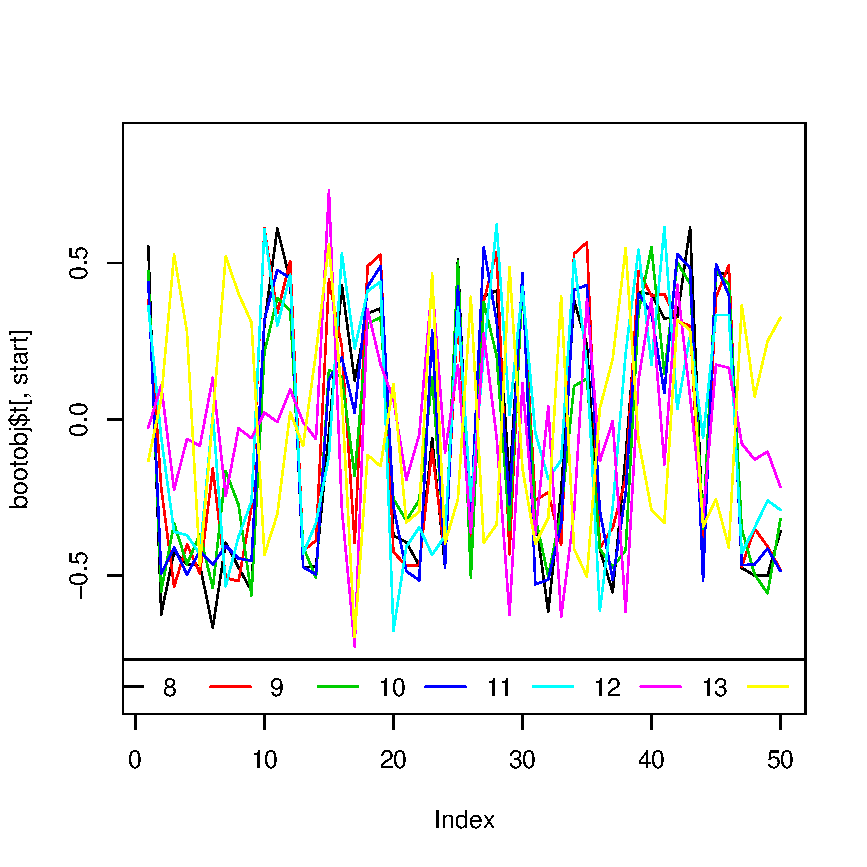
\includegraphics[width = 0.7\textwidth]{images/boottraceplot}
\caption{Trace of bootstrap iterations for first eigenvector}
\label{boottrace}
\end{center}
\end{figure}

It is quite clear that we need to invert some eigenvectors.   One approach is to identify one coefficient within an eigenvector and whenever this is below zero to multiply the entire vector by the scalar -1.   

\singlespacing
\begin{verbatim}
> idx <- hep.boot$t[,8] < 0
> hep.boot$t[idx,c(8:14)] <- hep.boot$t[idx,c(8:14)] * -1
> eigen.bootplot(hep.boot,8,7)
\end{verbatim}
\onehalfspacing

In this way we can obtain additional information on the variability of our principal component analysis.




\subsection{Other structure matrices}


We might also be interested in testing for other structure matrices, such as equi-correlation.   See \cite{Lawley:1963}.

\begin{eqnarray*}
\bar{r}_{k} = \frac{1}{p-1} \sum_{i=1; i \neq k}^{p} r_{ik}; k = 1, \ldots, p\\
\bar{r} = \frac{2}{p(p-1)} \sum_{i<k} \sum r_{ik}\\
\hat{alpha} = \frac{(p-1)^{2} \left[ 1 - (1 - \bar{r})^{2} \right] }{
p - (p - 2)(1 - \bar{r})^{2}}
\end{eqnarray*}

where $\frac{n-1}{(1-\bar{r})^{2}} \alpha$ follows a $T^{2}$ distribution.

Proof: JW 489  

\begin{verbatim}
mean(spot[lower.tri(spot)])
\end{verbatim}




\subsection{Forward search}

A more recent proposal for assessing the stability of principal component solution is the forward search \cite{Atkinson+etal:2004}.


\subsection{Assessing multivariate normality}
\label{mahalpca}

If we are prepared to entertain the idea that our data might be multivariate normal, it is very simple to obtain distance measures from the principal component scores and examine the adequacy of a representation in this context (clearly this might not be so useful if we are cannot assume multivariate normality).   Given a random vector $\boldsymbol{x}$ having mean $\boldsymbol{\mu}$ and covariance matrix $\boldsymbol{\Sigma}$, \cite{Flury:1997} (page 608-609) demonstrates the relationship between the principal component scores $z_{j}$ and the mahalanobis distance $\delta^{2}(\boldsymbol{x}, \boldsymbol{\mu})$ (which he calls the squared standard distance).   

\begin{theorem}
\begin{equation}
\label{Qstats}
\delta^{2}(\boldsymbol{x}, \boldsymbol{\mu}) = (\boldsymbol{x} -  \boldsymbol{\mu}) \boldsymbol{\Sigma}^{-1} (\boldsymbol{x} -  \boldsymbol{\mu}) = \sum_{j=1}^{p} \frac{z_{j}^{2}}{\lambda_{j}}
\end{equation}
where $\boldsymbol{z} = (z_{1}, \ldots, z_{p})^{T} = \boldsymbol{E}(\boldsymbol{x}- \boldsymbol{\mu})$, and $\boldsymbol{\Sigma} = \boldsymbol{E \Lambda E}^{T}$ as above.   
\end{theorem}
Proof: See \cite{Flury:1997}

We can use our principal component representation to partition the mahalanobis distance.   We want $\delta_{a}^{2} =  \sum_{j=1}^{q} \frac{z_{j}^{2}}{\lambda_{j}}$ corresponding to the distance encapsulated in our first $q$ principal components, and $\delta_{b}^{2} =  \sum_{j=q+1}^{p} \frac{z_{j}^{2}}{\lambda_{j}}$ corresponding to the distances encapsulated by the last $(p-q)$ principal components.   \cite{Flury:1997} indicates that these can be represented by $\chi^{2}$ random variables with respectively $q$ and $p-q$ degrees of freedom which lends itself to diagnostic assesment of the adequacy of the principal component representation.   It should perhaps be noted that this is a large sample approximation, \cite{Gnanadesikan:1977} (page 172) suggests $n = 25$ is adequate in the bivariate case.   \cite{Bilodeau+Brenner:1999} (page 186) therefore indicate the use of the Beta distribution, with $\alpha = \frac{p-2}{2p}$ and $\beta = \frac{n - p - 2}{2(n - p - 1)}$.   


It is possible to write a simple function to extract the distances associated with accepted and rejected principal component (and the total distance) which can then be used in various diagnostic plots.

\singlespacing
\begin{verbatim}
> princomp2dist <- function(obj.princomp, retain){
 scores <- t(t(obj.princomp$scores^2) / obj.princomp$sdev)
 dtot <- apply(scores, 1, sum)
 d1 <- apply(scores[,c(1:retain)], 1, sum)
 d2 <- apply(scores[,-c(1:retain)], 1, sum)
 dists <- data.frame(dtot = dtot, d1 = d1, d2 = d2)
 return(dists)
}

> hept.princomp <- princomp(hept.df[-1], scores = TRUE, scale = TRUE)
> ## form a princomp object
> hept.m <- princomp2dist(hept.princomp, 3)
> ## extract distances based on 3 component representation
\end{verbatim}
\onehalfspacing

Having obtained the distances, we only need some suitable method of investigation.   The most useful are qq-plots.   Given we have only 26 rows and 9 columns, we will use a modified verion of the \texttt{qqbeta} function given by \cite{Bilodeau+Brenner:1999}.   This plots the Mahalanobis distance against a suitable beta distribution.

\singlespacing
\begin{verbatim}
> qqbetaM <- function(x, p) {
  n <- length(x)
  a <- p/2
  b <- (n-p-1)/2
  alpha <- 0.5*(a-1)/a
  beta <- 0.5*(b-1)/b
  x <- sort(x)
  y <- qbeta(((1:n)-alpha)/(n-alpha-beta+1),a,b)*(n-1)^2/n
  plot(x,y,xlab="Mahalanobis distances",ylab="Beta quantiles")
}
> qqbetaM(hept.m$dtot,  7)
\end{verbatim}
\onehalfspacing

\begin{figure}
\begin{center}
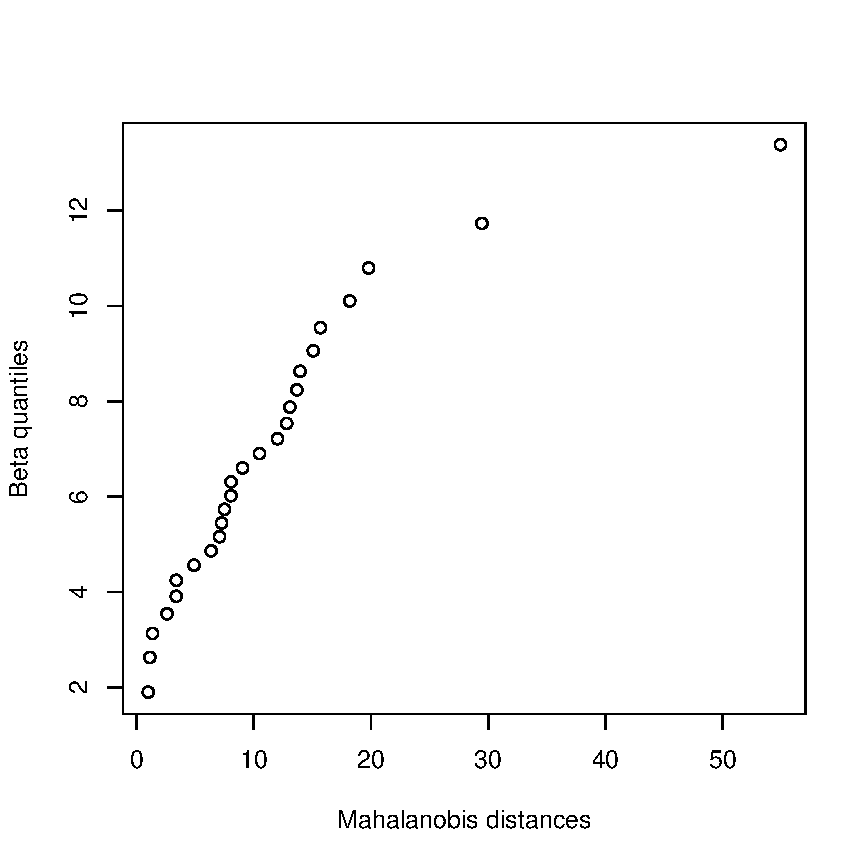
\includegraphics[width = 0.6\textwidth]{images/qqd1}
\caption{Mahalanobis distance from three component representation of the Heptathalon data versus theoretical quantiles of the Beta(1.5, 10) distribution}
\label{qqd1}
\end{center}
\end{figure}

It is reasonably clear from figure \ref{qqd1} that there are reasons to doubt multivariate normality, particularly in relation to outliers.    

Nevertheless, if we persevere, the adequacy of the $q=3$ dimensional representation can be considered.   Plotting $\delta_{a}^{2}$ against  $\delta_{b}^{2}$ provides one way of identifying those points not well represented by the three dimensional projection.

\singlespacing
\begin{verbatim}
> plot(hept.m$d1, hept.m$d2, 
  xlab = "Represented by q", ylab = "Not represented by q", 
  main = "Mahalanobis distances")
> identify(hept.m$d1, hept.m$d2, row.names(hept.df))
\end{verbatim}
\onehalfspacing

%It is equally possible to consider the mahalanobis distance in conventional desnsity plots.

%\singlespacing
%\begin{verbatim}
%library(MASS)
%truehist(hept.m$dtot, nbins = 9, ylim = c(0,0.1))
%curve(dchisq(x, df = 7), add = TRUE)
%\end{verbatim}
%\onehalfspacing

%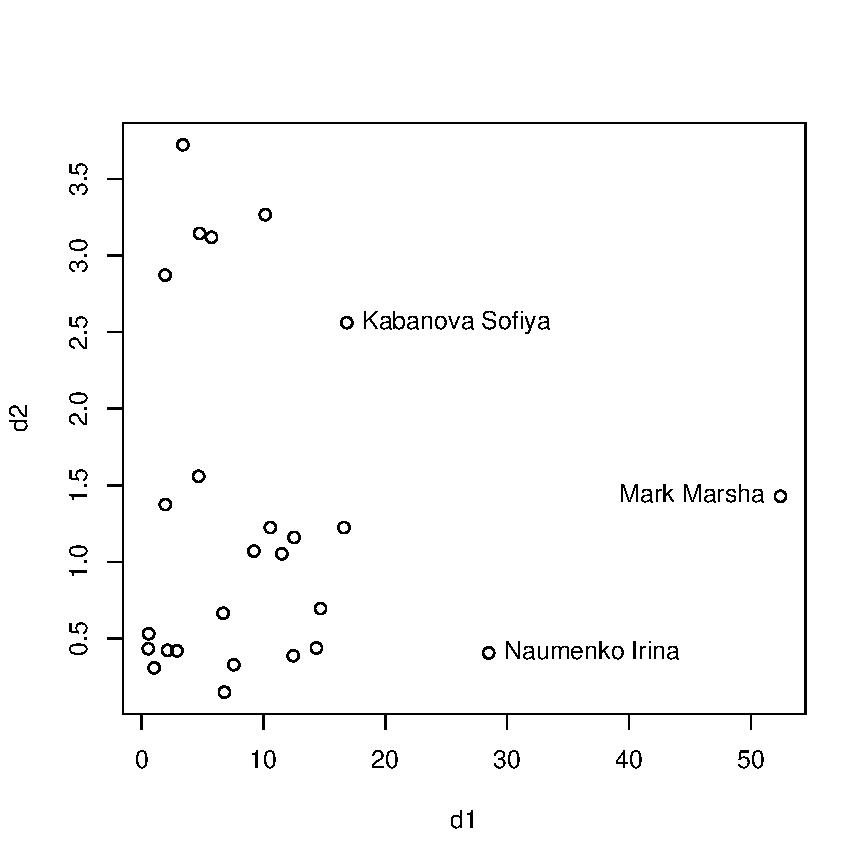
\includegraphics{images/d1d2}

%It should be noted that our ``outlier'' is only an outlier in the sense that she is not adequately represented by the first three principal components.   

However, qq plots of the data do tend to suggest that she could be considered an outlier.   This takes us back to the start of the chapter; in this case we may wish to consider a robust principal component analysis.

\singlespacing
\begin{verbatim}
> hep.princomp <- princomp(hept.df[-1], cor = TRUE)
> hep.cor.rob <- cov.rob(hept.df[,-1], cor = TRUE)$cor
> hep.princomp.rob <- princomp(cov = hep.cor.rob)
> hep.princomp
> hep.princomp.rob
> loadings(hep.princomp)
> loadings(hep.princomp.rob)
\end{verbatim}
\onehalfspacing

In this case it should be seen that there is only a slight difference between the estimates for the eigenvalues, but the loadings do alter somewhat.   Further methods for robust principal components will be considered in the next chapter.


\section{Interpreting the principal components}

This is the area that gets principal components a bad name.   Sometimes referred to as \textit{reification}, we look at the loadings on the various components, and try to suggest a concept that the component may be referring to.    Factor analysis does something similar.

It is worth at this point considering the correlation between a given variable and the principal component score (or projection of the data in $q$ dimensional subspace).

\begin{definition}
The univariate correlation between a variable and it's principal compnent projection can be given by:
\begin{displaymath}
\rho_{z,x_{k}} = \frac{e_{i}, \lambda_{i}}{\sqrt{\sigma_{kk}}}
\end{displaymath}
\end{definition}
\textbf{Proof}:[page 462] \cite{Johnson+Wichern:2002}

It should be noted that this only measures the unvariate contribution of $x$ to $z$, something \cite{Rencher:2002} feels is useless but something which may serve as a means to an end.

The corresponding measure for principal component analysis based on the correlation matrix is given by:
$\rho_{z, x_{standardised}} = e_{ik} \sqrt{\lambda_{i}}$


\section{Exercises}

\begin{enumerate}

\item Consider data $\boldsymbol{X} = \left( \begin{array}{ccc} 1 & 2 & 3 \\ 1 & 2 & 3 \end{array} \right) $.   Find the covariance and correlation matrix for these data.

\item Consider $\boldsymbol{S} = \left( \begin{array}{cc} 5 & 2 \\ 2 & 1 \end{array} \right) $.   Convert $\boldsymbol{S}$ into $\boldsymbol{R}$.   Calculate the principal components from each matrix.   Comare and contrast.   

\item Calculate $\rho_{z, x}$

\item S = diag(2,4,2), what are evals and evecs

\item Couple of questions on equicorrelation matrices

\item Estimate Sx and Sx.

\item Carapace data - how many pcs (sphericity test, bootstrap, scree, blah blah blah)

\end{enumerate}

%%% Local Variables: ***
%%% mode:latex ***
%%% TeX-master: "../book.tex"  ***
%%% End: ***


%\chapter{Contemporary topics in projection}   
%\label{projection}
\chapter{Extensions to Principal Component Methods}

\cite{Flury:1995} notes that in order to generalise principal components successfully, it is necessary to identify key properties of the method and define more general models where these properties are still valid.   He proposed an extension which retained an orthogonal transformation which maps correlated variables onto uncorrelated ones, this will be considered in section \ref{cpc}.   However, we also consider the principal curves approach which retains the self-consistency elements of principal components axes.   Firstly, we consider generalisations which attempt to deal with non-linearities in the data.

\section{Gnanadesikan's Generalised PCA}

One obvious extension to principal components was made by \cite{Gnanadesikan:1977}, and in a similar manner to polynomial regression adds quadratic and, where necessary, higher order terms to account for non-linearities in the day.   A conventional principal components analysis can then be carried out on this larger data set.   This technique has been succesfully demonstrated on artificial data lying on a circle, and is quite easy to implement:
\singlespacing
\begin{verbatim}
gpca <- function(X, ...){
 p <- dim(X)[2]
 p2 <- p + (p-1)*2
 counter <- p+1
    for (i in 1:p){
       for (j in i:p) {
           X[,counter] <- X[,i] * X[,j]
           counter <- counter + 1
                      }
                   }
  results <- prcomp(X, scale = TRUE, ...)
  return(results)
}

iris.gpca <- gpca(iris[,-5])
plot(iris.gpca$x[,1], gnad.iris$x[,2], 
  col = as.numeric(iris[,5]))
plot(iris.gpca)
biplot(iris.gpca)
\end{verbatim}
\onehalfspacing

Whilst polynomial regression has been successful, \cite{Flury:1995} notes that few publications feature this methodology.   The presence of linear and quadratic terms on different scales, different origins with a new metric may all bear little relationship to the distance from a curve in the original $p$-dimensional space.
We therefore consider some other proposals to extend the basic principal component approach.

\section{Simple Components}

Simple components analysis is very much an adaptation of the existing method to make the results more to interpret.  The original, optimal, principal components are replaced or supplements by simpler ones.
This procedure is a data analytical heuristic, so whilst principal components are by definition 100\% optimal, the user of the technique can adjust the results so that they are more easily understood but at the expense of reduced optimality.   A user judgement then has to be made as to whether the loss in optimality is justified given the ease of interpretation.   


We define the easier to interpret \emph{block-components} as those where all loadings are positive, and \emph{difference components} as those where some loadings are positive some are negative.   Most principal component analyses only contain one block-component, the simple component analysis allows the user to specify the number of block components to be fitted, provided the correlations among them are below some cut-off value (typically .3 or .4).   This is clearly a partitioning of the original untransformed variables, agglomerative hierarchical clustering is carried out at this stage.   Having done this, we only need to decide what we mean by simple difference comonents.   Those are obtained as simplified versions of some appropriate ``residual components''. The idea is to retain the large loadings (in absolute value) of these residual components and to shrink to zero the small ones. For each difference-component, the interactive procedure sca displays the loadings of the corresponding residual component (at the right side of the window), such that the user may know which variables are especially important for the definition of this component. 

At the third stage of the interactive procedure sca, it is possible to remove some of the difference-components from the system. 

For many examples, it is possible to find a simple system which is 90\% or 95\% optimal, and where correlations between components are below 0.3 or 0.4. When the structure in the correlation matrix is complicated, it might be advantageous to invert the sign of some of the variables in order to avoid as much as possible negative correlations. This can be done using the option `invertsigns=TRUE'. 

In principle, simple components can be calculated from a correlation matrix or from a variance-covariance matrix. However, the definition of simplicity used is not well adapted to the latter case, such that it will result in systems which are far from being 100\% optimal. Thus, it is advised to define simple components from a correlation matrix, not from a variance-covariance matrix. 

\singlespacing
\begin{verbatim}
X <- cor(iris[,-5])
sca(X)
 if(interactive()) {
+   r <- sca(cor(X), corblocks=0.4, qmin=5, interactive = TRUE)
+ }
\end{verbatim}
\onehalfspacing

\section{acpgen}

\section{Generalised principal components}

Further robust methods include proposals by \cite{Caussinus+Ruiz-Gazen:1993} which carries out a spectral analysis of a robust covariance matrix.


\singlespacing
\begin{verbatim}
library(amap)
X <- iris[,-5]
p <- acpgen(X,h1=1,h2=1/sqrt(2), scores = TRUE)

plot(p,main='ACP Iris data') ## the biplot

plot(p$scores[,1], p$scores[,2], col = as.numeric(iris[,5]), center = TRUE, reduce  TRUE)
\end{verbatim}
\onehalfspacing


A choice of kernels are available: gaussien: $\frac{1}{\sqrt{(2\pi)}} \exp(-u^{2}/2)$, quartic: $\frac{15}{16} (1-u^{2})^{2};  \mbox{if} |u| < 1$, triweight: $\frac{35}{32} (1-u^{2})^{3}; \mbox{if} |u| < 1$; epanechikov: $\frac{3}{4} (1-u^{2}) \mbox{if} |u| < 1$; cosinus: $\frac{\pi}{4} \cos (u \times \pi/2); \mbox{if} |u| < 1$ and require \verb+h+ to set the kernel bandwidth.   \verb+center+ and \verb+reduce+ set are binary indicators which centre and standardise the data.   



%    sdev: the standard deviations of the principal components.
%
%   loadings: the matrix of variable loadings (i.e., a matrix whose columns
%      contain the eigenvectors).  This is of class '"loadings"':
%          see 'loadings' for its 'print' method.
%
%  scores: if 'scores = TRUE', the scores of the supplied data on the
%          principal components.
%
%     eig: Eigen values





\section{Kernel Based Methods}

Kernel methods are widely used in many multivariate applications, formal proposals for their use in connection with principal components seem to be much more recent.   \cite{Schoelkopf+etal:1998} made proposals for the use of kernels in eigen analysis which can be used as a form of non-linear principal component analysis.   This method has been made available within the \verb+kernlab+ library \cite{Karatzoglou+etal:2005} in \textbf{R}.   It should perhaps be noted that kernel solutions increase the computer power associated with analysis of a dataset of given dimensionaltiy.
   
Any kernel  function which computes a dot product between two vectors can be used, these are either specified by the name of a user defined function or by using one of the inbuilt kernel functions which include \verb+rbfdot+, a Gaussian radial basis kernel function and  \verb+laplacedot+, a Laplacian kernel function.   These  both require the inverse kernel width \verb+sigma+ to be specified by \verb+par = list(sigma)+.  Other kernels include \verb+polydot+, a polynomial kernel function requiring the parameters \verb+kpar = list(degree, scale, offset)+; \verb+vanilladot+,a linear kernel function; \verb+tanhdot+, a hyperbolic tangent kernel function which requires \verb+kpar = list(scale, offset)+ to be set; \verb+besseldot+, a Bessel kernel function requiring  \verb+kpar = list(sigma, order, degree)+ to be set.

A couple of points need to be noted.   \verb+features+ specifies the number of features to be retained, as  kernel method these aren't the same as the conventional form of principal components.   The default value of \verb+0+ therefore produces rather a large number of components, which can be limited by an argument to \verb+th+, set by default to 0.0001.   Again, this can't be considered in the same way as for say, the Kaiser criterion. 





Consider an example with Fisher's Iris data.   We extract two principal components (\verb+features=2+), and select a Gaussian kernel with an inverse kernel width of 0.2

\begin{verbatim}
\library(kernlab)
data(iris)
test <- sample(1:150,20)

kpc <- kpca(~.,data=iris[-test,-5],
    kernel="rbfdot", kpar=list(sigma=0.2), features=2)
pc <- prcomp(~.,data=iris[-test,-5] )

par(mfrow = c(1,2))
plot(pc$x[,1], pc$x[,2], col = as.integer(iris[-test,5]), 
    xlab="1st Principal Component",ylab="2nd Principal Component",
    main = "Conventional pca")

emb <- predict(pc, iris[test, -5])
points(emb,pch=as.numeric(iris[test,5]))

plot(rotated(kpc), col=as.integer(iris[-test,5]),
    xlab="1st Principal Component",ylab="2nd Principal Component",
    main = "Kernel PCA")

emb <- predict(kpc,iris[test,-5])
points(emb,pch=as.numeric(iris[test,5]))
\end{verbatim}

It should be noted that the \verb+kernlab+ package has been set out following S4 classes.   Therefore, whilst it is possible to extract eigenvalues from conventional principal components using \verb+pc$sdev^2+ (note that, as implied by its name, \verb+sdev+ returns the square roots of the eigenvalues), when using \verb+kernlab+ the extractor functons have to be used.   Therefore, \verb+eig(kpc)+ will give the eigenvalues from the kernel based decomposition.

\begin{figure}
\begin{center}
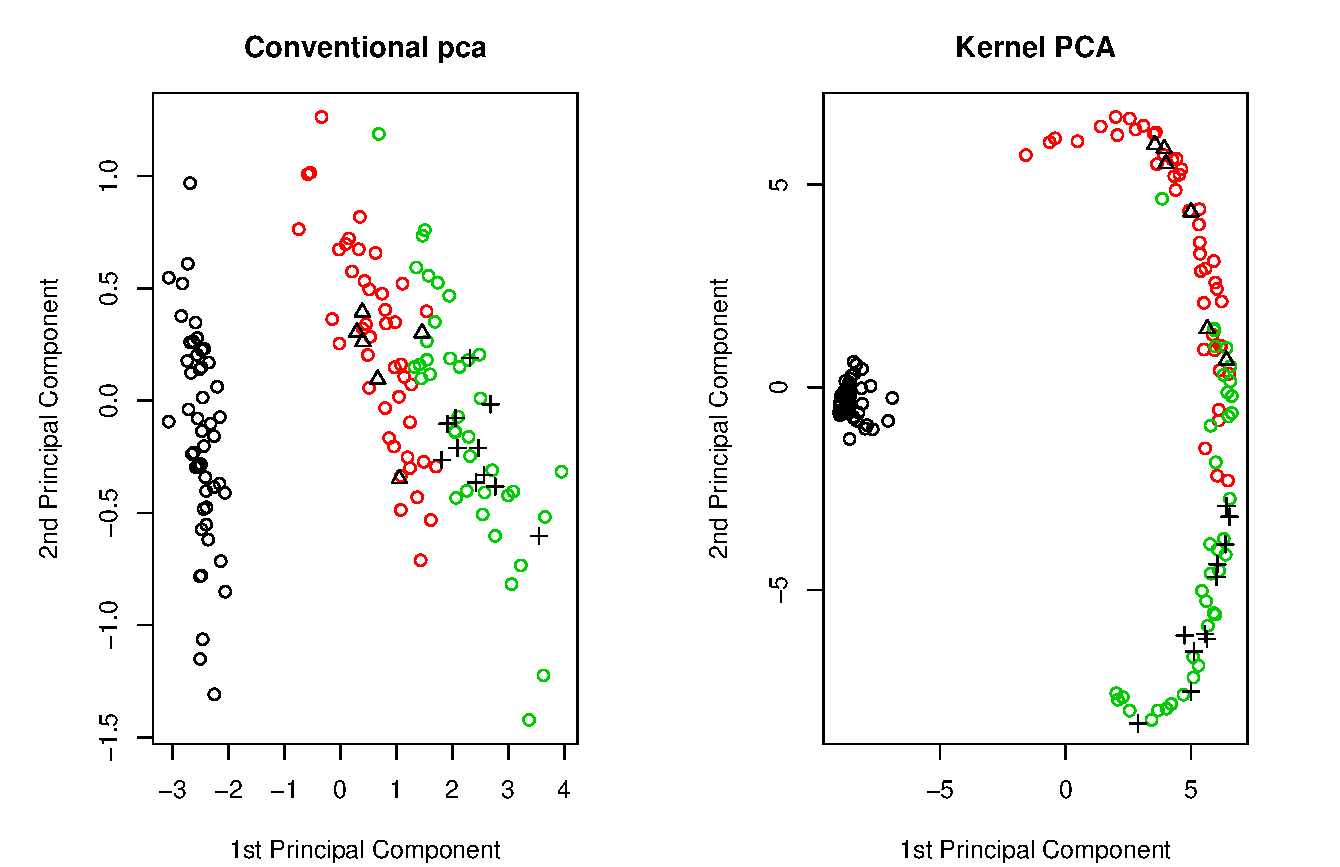
\includegraphics[width = 0.8\textwidth]{images/kernelpca}
\caption{Projection from conventional and kernal pca}
\label{kernpca}
\end{center}
\end{figure}


\section{Principal Curve Analysis}

\singlespacing
\begin{verbatim}
library(pcurve)
par(mfrow = c(3,2), cex = 0.5)
spec.fit <- pcurve(iris[,-5], start = "pca", plot.init = FALSE, plot.segs = FALSE, plot.resp = FALSE, maxit = 5)
\end{verbatim}
\onehalfspacing

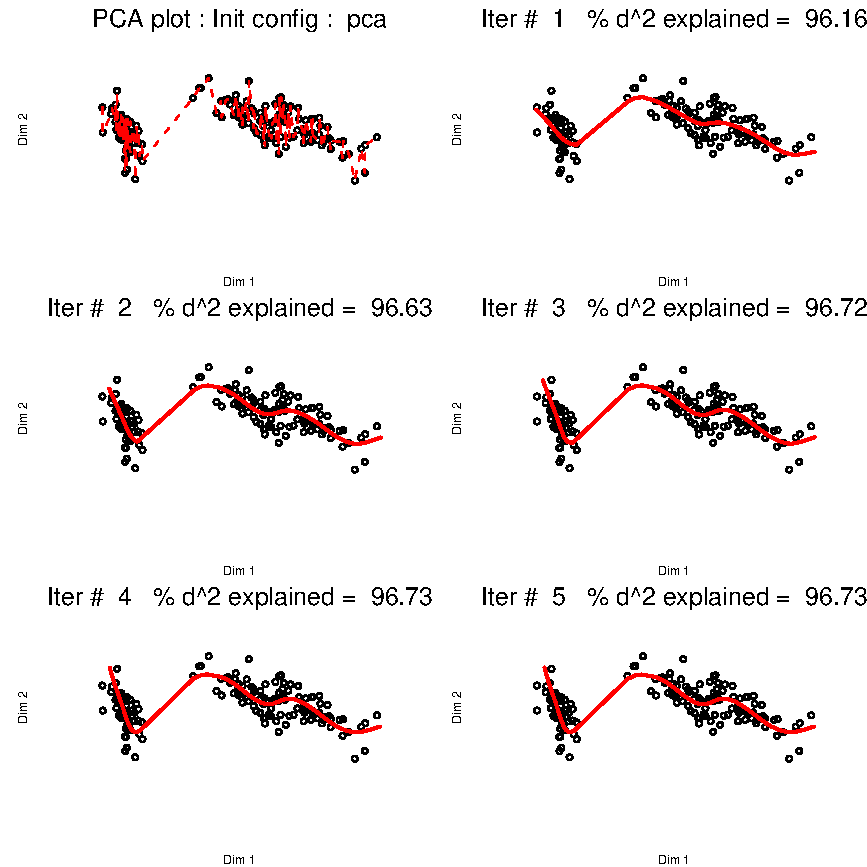
\includegraphics[width = 0.7\textwidth]{images/irispcurve}

This does beg the question as to whether we should be performing one or three principal component analyses.   This generalisation of the technique will be considered in the next section.


\section{Principal components for more than one data set}
\label{cpc}

Finally, we consider principal components for more than one set of data, as discussed before this is a clear generalisation of the principal component technique.   Given the largely data analytic rationale for principal components analysis which dominates the discussion in chapter \ref{pca} it is perhaps understandable that models which could deal with covariance matrices arising from related but separate groups had not been developed.   Although \cite{Jolicoeur:1963} considered data from male and female turtles their analysis was essentially separate and informal comparisons were made between the groups.   Formal comparison of group specific principal components was first proposed by \cite{Krzanowski:1980} who examined the angles between eigenvectors.   He found that an optimum could be found by carrying out a spectral decomposition of:
\begin{equation}
\boldsymbol{H} = \sum_{i=1}^{k}\boldsymbol{L}_{i}^{T}\boldsymbol{L}_{i}
\end{equation}
where $\boldsymbol{L}_{i}$ are the $p \times q$ matrices of eigenvectors for each group $i$.   This method however does not weight the matrices $\boldsymbol{L}_{i}$ regardless of possibly different sample size and does not adequately account for instabilities in eigenvectors.

A formal model for simultaneous analysis has been proposed by \cite{Flury:1984}, which assumes common eigenvectors but group specific eigenvalues.

\begin{displaymath}
\boldsymbol{\Sigma}_{i} = \boldsymbol{E} \boldsymbol{\Lambda}_{i}  \boldsymbol{E}^{T}
\end{displaymath}
which assumes parallel ellipses of potentially different size.

This method continues to be updated with recent proposals by \cite{Boik:2002}.  However, the CPC model is readily demonstrated within \textbf{R}.








%
%library(grid)
% pltSplomT(USArrests,mainL="",hist="b",adjust=0.4,cex.diag = 0.7)
%library(cwhplot)










%%% Local Variables: ***
%%% mode:latex ***
%%% TeX-master: "../book.tex"  ***
%%% End: ***


An outline of probabilistic PCA, Independence Components Analysis, 
Dimension reduction regression (SIR, PLS, Redundancy Analysis)




\chapter{Canonical Correlation}
\label{cancor}

\section{Canonical variates}
\label{canvar}

\section{Interpretation}
\label{canint}
%%%%%\chapter{Canonical Correlation}

In canonical correlation, we are interested in the relationship between two sets of variables.   We do this by creating linear combinations $\boldsymbol{U} = \boldsymbol{a_{1} x_{1}} + \boldsymbol{a_{2} x_{2}} + \cdots + \boldsymbol{a_{p} x_{p}}$ and  $\boldsymbol{V} = \boldsymbol{b_{1} y_{1}} + \boldsymbol{b_{2} y_{2}} + \cdots + \boldsymbol{b_{q} y_{q}}$ such that the correlation between $\boldsymbol{U}$ and $\boldsymbol{V}$ is as high as possible.


To do this, we need to work out the correlation matrix, and partition it:


\begin{displaymath}
\begin{array}{ccccccc} & x_{1} & \ldots & \_{p} & y_{1} & \ldots & y_{q} \end{array}
\end{displaymath}
\begin{displaymath}
\begin{array}{c} x_{1} \\ \vdots \\ x_{p} \\y_{1} \\ \vdots \\y_{3}\end{array}
\left( \begin{array}{ccc|ccc} &&&&&\\&A_{p \times p}& &C_{p \times q}&\\&&&&&\\
\hline
&&&&&\\&C_{q \times p}& &B_{q \times q}&\\&&&&&\\ \end{array} \right)
\end{displaymath}

Having done this, we calculate the matrix:

\begin{displaymath}
\boldsymbol{B^{-1}C^{T}A^{-1}C}
\end{displaymath}

and find the associated eigenvalues (in descending order)  $\lambda_{1} > \lambda_{2} > \ldots > \lambda_{r}$.   The corresponding eigenvectors $\boldsymbol{b_{1}}, \boldsymbol{b_{2}}, \ldots, \boldsymbol{b_{r}}$ give the coefficients of the Y variables.

So: 

\begin{displaymath}
\boldsymbol{v_{i}} = \boldsymbol{b_{i}^{T}} \boldsymbol{Y}
\end{displaymath}

where $\boldsymbol{b_{i}} = \left(\begin{array}{c} b_{i1} \\ \vdots \\ b_{iq} \end{array} \right)$ and $\boldsymbol{Y} = \left(\begin{array}{c} \boldsymbol{y_{1}} \\ \vdots \\ \boldsymbol{y_{q}} \end{array} \right)$, or in longhand:

\begin{displaymath}
\boldsymbol{v_{i}} = b_{i1} \boldsymbol{y_{1}} + \cdots + b_{iq} \boldsymbol{y_{q}}
\end{displaymath}

Having calculated these, it is possible to solve the coefficients for the X variables:

$a_{1} = \boldsymbol{A^{-1} C b_{1}}, a_{2} = \boldsymbol{A^{-1} C b_{2}}, \ldots,  a_{r} = \boldsymbol{A^{-1} C b_{r}}$,

f
\begin{displaymath}
\boldsymbol{u_{i}} = \boldsymbol{a_{i}^{T}} \boldsymbol{X}
\end{displaymath}


where $\boldsymbol{a_{i}} = \left(\begin{array}{c} a_{i1} \\ \vdots \\ a_{iq} \end{array} \right)$ and $\boldsymbol{X} = \left(\begin{array}{c} \boldsymbol{x_{1}} \\ \vdots \\ \boldsymbol{x_{r}} \end{array} \right)$, or in longhand:

\begin{displaymath}
\boldsymbol{u_{i}} = a_{i1} \boldsymbol{x_{1}} + \ldots + a_{ir} \boldsymbol{x_{r}}
\end{displaymath}

And one really cute result is that $\left[corr(\boldsymbol{u_{i}}, \boldsymbol{v_{i}})\right]^{2} = \lambda_{i}$.

\section{Computer example}

Franco Modigliani proposed a life cycle savings model, the savings ratio (aggregate personal saving divided by disposable income) is explained by per-capita disposable income, the percentage rate of change in per-capita disposable income, and two demographic variables: the percentage of population less than 15 years old and the percentage of the population over 75 years old. 

However, we are interested here in the relationship between the two demographic variables (percent of population under 15, percent of population over 75) and the three financial variables (personal savings, per-capita disposal income, growth rate of dpi).   The first stage of any such analysis would be a visual inspection.


\begin{verbatim}
pairs(LifeCycleSavings, pch = 16)
\end{verbatim}

\begin{figure}
\begin{center}
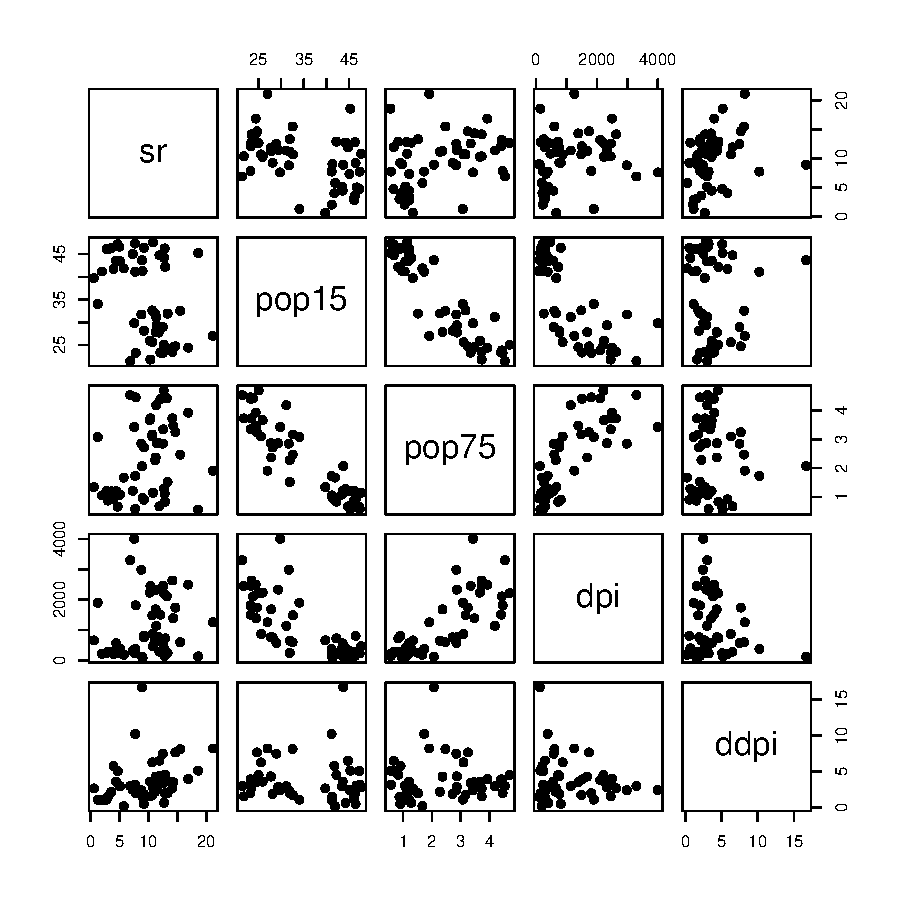
\includegraphics[width = 0.6\textwidth]{images/cancor}
\caption{Pairwise scatterplots of Life Cycle Savings data}
\end{center}
\end{figure}

And it is worth examining the correlation matrix:

\singlespacing
\begin{verbatim}
> cor(LifeCycleSavings)
              sr       pop15       pop75        dpi        ddpi
sr     1.0000000 -0.45553809  0.31652112  0.2203589  0.30478716
pop15 -0.4555381  1.00000000 -0.90847871 -0.7561881 -0.04782569
pop75  0.3165211 -0.90847871  1.00000000  0.7869995  0.02532138
dpi    0.2203589 -0.75618810  0.78699951  1.0000000 -0.12948552
ddpi   0.3047872 -0.04782569  0.02532138 -0.1294855  1.00000000
\end{verbatim}
\onehalfspacing

It appears that the \textbf{X} variables are correlated.   This is less so for \textbf{Y} variables, and even less so for \textbf{X,Y} inter-correlations.

You need to be sure that the variables are \emph{scaled} before carrying out a canonical correlation analysis.   

\singlespacing
\begin{verbatim}
LifeCycleSavingsS <- scale(LifeCycleSavings)
pop <- LifeCycleSavingsS[, 2:3] ## The X matrix
oec <- LifeCycleSavingsS[, -(2:3)] ## the Y matrix
\end{verbatim}
\onehalfspacing

Having created an \textbf{X} matrix and a \textbf{Y} matrix, we now want to find linear combinations of \textbf{X} which have maximum correlation with \textbf{Y}.

\singlespacing
\begin{verbatim}
> cancor(pop, oec)
$cor
[1] 0.8247966 0.3652762

$xcoef
             [,1]       [,2]
pop15 -0.08338007 -0.3314944
pop75  0.06279282 -0.3360027

$ycoef
           [,1]        [,2]         [,3]
sr   0.03795363  0.14955310 -0.023106040
dpi  0.12954600 -0.07518943  0.004502216
ddpi 0.01196908 -0.03520728  0.148898175

$xcenter
        pop15         pop75 
-4.662937e-16  2.753353e-16 

$ycenter
          sr          dpi         ddpi 
1.421085e-16 6.661338e-17 4.440892e-16 
\end{verbatim}
\onehalfspacing

This indicates one canonical correlate with a correlation of 0.8247966 between $z_{\boldsymbol{X}1}$ and $z_{\boldsymbol{Y}1}$

\begin{eqnarray}
z_{\boldsymbol{X}1} =  -0.08338007  x_{pop15} + 0.06279282 x_{pop75}\\
z_{\boldsymbol{Y}1} = 0.03795363 y_{sr} + 0.12954600 y_{dpi} +  0.01196908 y_{ddpi}
\end{eqnarray}

If we extract the coefficients as vectors (this time we have created \texttt{LCS.cancor} as an object; also we have used \texttt{as.numeric(\ldots)} to extract the coefficients in a form suitable for matrix multiplication).

\singlespacing
\begin{verbatim}
> LCS.cancor <- cancor(pop, oec)
> ycoef <- as.numeric(LCS.cancor$ycoef[,1])
> xcoef <- as.numeric(LCS.cancor$xcoef[,1])
> v1 <-  oec %*% ycoef ## remember oec and pop are scaled
> u1 <-  pop %*% xcoef
> plot(v1, u1)
> identify(v1, u1, row.names(LifeCycleSavings))
\end{verbatim}
\onehalfspacing


\subsection{Interpreting the canonical variables}

There is some ``controversy'' about the best way of interpreting the canonical variables.   You have two possibilities:

\begin{itemize}
\item Interpret the coefficients in a similar way to that used in principal components (problems with collinear variables)
\item Calculate the correlation between the canonical and the original variables (doesn't tell you anything about joint contributions)
\end{itemize}

%Consider:

%$\rho_{\hat{U},\boldsymbol{x}}$ = matrix of correlations between $\hat{U}$ and $\boldsymbol{x}$\\ 
%$\rho_{\hat{V},\boldsymbol{y}}$ = matrix of correlations between $\hat{V}$ and $\boldsymbol{y}$ \\
%$\rho_{\hat{U},\boldsymbol{y}}$ = matrix of correlations between $\hat{U}$ and $\boldsymbol{y}$ \\
%$\rho_{\hat{V},\boldsymbol{x}}$ = matrix of correlations between $\hat{V}$ and $\boldsymbol{x}$\\ 

%Which can be obtained fairly simply as:

%\begin{eqnarray*}
%\rho_{\hat{U},\boldsymbol{x}} = a \Sigma_{11}



\subsection{Hypothesis testing}

As with Principal Components, a certain amount of hypothesis testing is possible.   The distributional properties of canonical variables is far wilder than principal components - none of the recommended books discuss it.   However, the tests can be described.   For example, if we wanted to test whether there was any relationship between our two sets of variables:

\begin{displaymath}
H_{0}; \boldsymbol{\Sigma}_{12} = \boldsymbol{0}
\end{displaymath}

The Likelihood ratio test leads us to:

\begin{displaymath}
\Lambda^{\frac{2}{n}} = |\boldsymbol{I} - \boldsymbol{S_{22}^{-1}}\boldsymbol{S_{21}}\boldsymbol{S_{11}^{-1}}\boldsymbol{S_{12}}| = \prod_{i=1}^{k}(1-r_{i}^{2}) \sim \Lambda_{Wilks}(p, n-1-q,q)
\end{displaymath}

Using Bartlett's approximation this can yield a $chi^{2}$ test:

\begin{displaymath}
-\left(n-\frac{1}{2}(p+q+3)\right) \log \prod_{i=1}^{k}(1-r_{i}^{2}) \sim \chi^{2}_{pq}
\end{displaymath}


As we've seen before, perhaps we are more interested in finding out how many canonical correlations we need to keep in our analysis.   Bartlett also proposed a statistic only $s$ canonical correlations are non-zero:

\begin{displaymath}
-\left(n-\frac{1}{2}(p+q+3)\right) \log \prod_{i=s+1}^{k}(1-r_{i}^{2}) \sim \chi^{2}_{(p-s)(q-s)}
\end{displaymath}

%%% Local Variables: ***
%%% mode:latex ***
%%% TeX-master: "book.tex"  ***
%%% End: ***

 


\chapter{Factor analysis}
\label{factanal}

\section{Role of factor analysis}
\label{rolefa}

Most of the development of factor analysis has taken place outside the statistical community, most often in terms of Psychometrics which may partly reflect its origins in the study of intelligence.   The earliest cited reference is \cite{Spearman:1904}.  Factor Analysis and Principal Components Analysis are often confused with each other, just to be really awkward there is one method of performing Factor Analysis called Principal Component Extraction.   The two methods should never be confused.   Principal Components seeks orthogonal projections of the data according the variance maximisation with the hope of achieving some dimension reduction.   Factor analysis is all about studying the co-variance (or correlation) and is based on a statistical model.  We hope to describe the covariance relationships between many variables in terms of a few underlying, unobservable random quantities called factors.   If there is a group of highly correlated variables, which in turn are uncorrelated with other variables, perhaps these represent realisations of some underlying phenomena that is responsible for for the observed correlations.   It is an attempt to approximate the covarariance matrix $\boldsymbol{\Sigma}$.  It is not highly regarded by many statisticians, but it is used by many others.   There are currently many variations on a theme (such as Structural Equation Modelling) which are also very common in many applied literatures.



Whilst we can consider one model for factor analysis, there are two very different fitting methods, neither of which is entirely satisfactory.   Having found a solution there are a large number of possible rotations of the solution each of which aim to give the most interpretable solution.   In other words, don't be surprised if different computer programs give different ``Factor Analysis'' solutions for the same data.


\begin{figure}
\begin{picture}(100,200)(0,0)

\put(0,150){\fbox{f1}}
\put(30,150){\vector(2,-1){95}} 
\put(30,150){\vector(2,1){95}} 
\put(30,150){\vector(1,-1){95}} 

\put(0,50){\fbox{f2}}
\put(30,50){\vector(2,-1){95}} 
\put(30,50){\vector(2,1){95}} 
\put(30,50){\vector(1,1){95}}  

\put(150,0){\fbox{X1}}
\put(150,100){\fbox{X2}}
\put(150,200){\fbox{X3}}

\end{picture}
\caption{Factor analysis, dependence between three variables represented by two latent variables - is this sensible}
\end{figure}

Factor Analysis is normally carried out with a view to reification: the investigator usually has a conceptual model of some underlying entity which cannot be measured directly.   These latent, or hidden, variables are the factors in factor analysis.   The aim of factor analysis is that each of the $p$ observed variables can be represented by means of $q<p$ mutually uncorrelated common factors.   This will leave some uncorrelated residual specific to each of the observed variables, the uniqueness, which is not correlated with any of the remaining $p-1$ variables \footnote{Note that the diagonal of a correlation matrix is 1. This statement implies that only part of this 1 is due to the $q<p$ latent variables - this part is known as the communality.}.   It is possible to rotate the $q$ axes of common factors to new orthogonal or obligue axes to make the factor solution fit with existing theoretical ideas regarding the model.  

\section{The factor analysis model}
\label{factanalmodel}

The orthogonal model underlying Factor Analysis can be described as follows:

\begin{displaymath}
\label{factanal}
\boldsymbol{x} = \boldsymbol{\mu} + \boldsymbol{\Gamma} \boldsymbol{\phi} + \boldsymbol{\zeta}
\end{displaymath}

Where $\boldsymbol{x}$ is an $1 \times p$ random vector.   $\boldsymbol{\mu}$ represents a vector of unknown constants (mean values), $\boldsymbol{\Gamma}$ is an unknown $p \times q$ matrix of constants referred to as the \textit{loadings}.   $\boldsymbol{\phi}$ is a $q \times 1$ unobserved random vector referred to as the \textit{scores} assumed to have mean $\boldsymbol{0}$ and covariance $\boldsymbol{\Sigma}_{\phi}$, it is commonly assumed that $\boldsymbol{\Sigma}_{\phi} = \boldsymbol{I}$.   $\boldsymbol{\zeta}$ is $1 \times p$ unobserved random error vector having mean $\boldsymbol{0}$ and by assumption a diagonal covariance $\boldsymbol{\psi}$ referred to as the \textit{uniqueness} or \textit{specific variance}.   

With these assumptions, $cov(\boldsymbol{\phi}, \boldsymbol{\zeta}) = 0$, if $\boldsymbol{\Sigma}_{\phi} = \boldsymbol{I}$ then $cov(\boldsymbol{x}, \boldsymbol{\phi}) = \boldsymbol{\Gamma}$.   It is worth emphasising that unlike many multivariate techniques covered here, factor analysis is a statistical model for our observations, with the following distributional form:

\begin{displaymath}
\boldsymbol{x} \sim Normal(\boldsymbol{\mu}, \boldsymbol{\Gamma} \boldsymbol{\Gamma}^{T} + \boldsymbol{\psi})
\end{displaymath}

It may be slightly clearer to consider the way a vector of observations $\boldsymbol{x} = x_{1}, \ldots, x_{p}$ are modelled in factor analysis:

\begin{eqnarray*}
x_{1} &=& \mu_{1} + \sum_{k=1}^{q} \gamma_{1k} \phi_{k}  + \zeta_{1}\\
x_{2} &=& \mu_{2} + \sum_{k=1}^{q} \gamma_{2k} \phi_{k}  + \zeta_{2}\\
&\vdots&\\
x_{p} &=& \mu_{p} + \sum_{k=1}^{q} \gamma_{pk} \phi_{k}  + \zeta_{p}
\end{eqnarray*}

Note that under the terms of this model:

\begin{equation}
\label{communalities}
var(x_{j}) = \gamma_{j1}^{2} + \gamma_{j2}^{2} + \ldots + \gamma_{jq}^{2} + var(\zeta_{j})
\end{equation} 

One potential problem with this model should be immediately obvious, there can be rather more parameters than data.   For example, note that the covariance matrix $\boldsymbol{\Sigma}$ has $p(p+1)/2$ parameters, the factor model $ \boldsymbol{\Gamma} \boldsymbol{\Gamma}^{T} + \boldsymbol{\psi})$ has $qp - q(q-1)/2 + p$ parameters.  One issue arises whereby a factor analsis model must be constrained in order to ensure identifiability.  Clearly, $p(p+1)/2 \geq qp - q(q-1)/2 + p$, or:

\begin{equation}
\label{qp}
q \leq \frac{2p + 1 - \sqrt{8p-1}}{2}
\end{equation}

This gives some maximum values of $q$ for given values of $p$:


\begin{tabular}{rr}
\hline
$p$ & max $q$ \\
\hline
1 & 0\\
2 & 0\\ 
3 & 1\\
4 & 1\\
5 & 2\\
6 & 3\\
7 & 3\\
8 & 4\\
9 & 5\\
10 & 6\\
\hline
\end{tabular}

Where $q<p$, the right hand side of \ref{communalities} indicates how much of $var(x_{j}$ is explained by the model, a concept referred to as the communality.   Consideration of the order of the model leads on to a point we will consider later, degrees of freedom after fitting a $q$ factor model:

\begin{equation}
\label{dffact}
df = \frac{p(p+1)}{2} - qp + \frac{q(q-1)}{2} - p = \frac{(p-q)^{2} - (d+m)}{2}
\end{equation}


\subsection{Centred and standardised data}

In practice it is often much simpler to centre the data, so that we model:

\begin{equation}
\label{facentre}
x_{j} - \mu_{j} = \sum_{k=1}^{q} \gamma_{k} \phi_{k} + \zeta_{j}; j = 1, \ldots, p
\end{equation}

or even to standardise the variables so that in effect we are modelling the correlation matrix rather than the covariance matrix.   

\begin{equation}
\label{fastandardise}
\frac{x_{j} - \mu_{j}}{\sigma_{jj}} = \sum_{k=1}^{q} \gamma_{k} \phi_{k} + \zeta_{j}; j = 1, \ldots, p
\end{equation}


Regardless of the data matrix used, factor analysis is essentially a model for $\boldsymbol{\Sigma}$, the covariance matrix of $\boldsymbol{x}$, 

\begin{displaymath}
\label{covdecomp}
\boldsymbol{\Sigma} = \boldsymbol{\Gamma}\boldsymbol{\Gamma}^{T} + \boldsymbol{\psi}
\end{displaymath}

\subsection{Factor indeterminacy}

We now consider another problem with factor analysis.   It is a very indeterminate model, specifically it is unchanged if we replace $\boldsymbol{\Gamma}$ by $\boldsymbol{K} \boldsymbol{\Gamma}$ for any orthogonal matrix $\boldsymbol{K}$.   However, this can be turned to our advantage, with sensible choice of a suitable orthogonal matrix $\boldsymbol{K}$ we can achieve a rotation that may yield a more interpretable answer.  Factor analysis therefore requires an additional stage, having fitted the model we may wish to consider rotation of the coefficients.  

\subsection{Strategy for factor analysis}

 To fit the model, we therefore need to:

\begin{itemize}
\item Estimate the number of common factors $q$.   
\item Estimate the factor loadings $\boldsymbol{\Gamma}$
\item Estimate the specific variances $\boldsymbol{\psi}^{2}$
\item On occasion, estimate the factor scores $\boldsymbol{\phi}$
\end{itemize}


We will now consider fitting methods for factor analysis.   It will be obvious that the preferred method in R is the maximum likelihood method, but we will first consider methods based around principal components to reinforce some ideas about the model.

\section{Principal component extraction}

We have already used the spectral decomposition to obtain one possible factoring of the covariance matrix $\boldsymbol{\Sigma}$.

\begin{displaymath}
\boldsymbol{\Sigma} = \boldsymbol{E} \boldsymbol{\Lambda}\boldsymbol{E}^{T}
\end{displaymath}

which can be expanded:

\begin{eqnarray*}
\boldsymbol{\Sigma} &=& \lambda_{1} \boldsymbol{e}_{1} \boldsymbol{e}_{1}^{T} +  \lambda_{2} \boldsymbol{e}_{2} \boldsymbol{e}_{2}^{T} + \ldots  \lambda_{p} \boldsymbol{e}_{p} \boldsymbol{e}_{p}^{T} \\
 &=& \left( \sqrt{\lambda_{1}} \boldsymbol{e}_{1}, \sqrt{\lambda_{2}} \boldsymbol{e}_{2}, \ldots, \sqrt{\lambda_{p}} \boldsymbol{e}_{p} \right) \left( \begin{array}{c} \sqrt{\lambda_{1}} \boldsymbol{e}_{1} \\  \sqrt{\lambda_{2}} \boldsymbol{e}_{2} \\ \vdots \\  \sqrt{\lambda_{p}} \boldsymbol{e}_{p} \end{array} \right)
\end{eqnarray*}

Of course, in practice we don't know $\boldsymbol{\Sigma}$ and we use  $S$ (or we standardise the variables and use $R$ - it should be remembered that this is rather a big decision when working with principal components).   Referring back to our data, it should be remembered that the spectral decomposition yields linear principal components as follows:

\begin{eqnarray*}
z_{1} &=& e_{11}x_{1} + e_{12}x_{2} + \ldots + e_{1p} x_{p}; var(z_{1})=\lambda_{1}\\
z_{2} &=& e_{21}x_{2} + e_{22}x_{2} + \ldots + e_{2p} x_{p}; var(z_{2})=\lambda_{2}\\
&\vdots&\\
z_{p} &=& e_{p1}x_{1} + e_{p2}x_{1} + \ldots + e_{1p} x_{p}; var(z_{p})=\lambda_{p}
\end{eqnarray*}

which in matrix notation this can be expressed as: 

\begin{equation}
\label{pcfact}
\boldsymbol{Z} = \boldsymbol{E}\boldsymbol{X}
\end{equation}

where  $\boldsymbol{Z} = \left( \begin{array}{c} z_{1} \\ z_{2} \\ \vdots \\ z_{p} \end{array} \right)$,  $\boldsymbol{X} = \left( \begin{array}{c} X_{1} \\ X_{2} \\ \vdots \\ X_{p} \end{array} \right)$ and  $\boldsymbol{E} = \left( \begin{array}{cccc} e_{11} & e_{12} & \hdots & e_{1p} \\ 
e_{21}& e_{22} & \hdots & e_{2p} \\
 \vdots & \vdots & \ddots & \vdots \\ 
e_{p1} & e_{p2} & \hdots & e_{pp}  \end{array} \right)$.   

Multiplying both sides of \ref{pcfact} by $\boldsymbol{E}^{-1}$gives:

\begin{equation}
\boldsymbol{E}^{-1} \boldsymbol{Z} = \boldsymbol{X}
\end{equation}

We know orthogonal matrices generally that $\boldsymbol{E}^{-1} = \boldsymbol{E}^{T}$ so we can invert the transformation by using

\begin{equation}
\boldsymbol{X} = \boldsymbol{E}^{T} \boldsymbol{Z}
\end{equation}

which can be expanded as:

\begin{eqnarray*}
x_{1} &=& e_{11}z_{1} + e_{21} z_{2}  + \ldots + e_{p} z_{p}  \\
x_{2} &=& e_{12}z_{2} + e_{22} z_{2} + \ldots + e_{p} z_{p}  \\
&\vdots& \\
x_{p} &=& e_{1p}z_{1} + e_{2p} z_{2} + \ldots + e_{pp} z_{p}  
\end{eqnarray*}

which we could express as;

\begin{eqnarray*}
x_{1} &=& (e_{11} \sqrt{\lambda_{1}}) \frac{z_{1}}{\sqrt{\lambda_{1}}} + (e_{21} \sqrt{\lambda_{2}}) \frac{z_{2}}{\sqrt{\lambda_{2}}} + \ldots +  (e_{p1} \sqrt{\lambda_{p}}) \frac{z_{p}}{\sqrt{\lambda_{p}}} \\
x_{2} &=& (e_{12} \sqrt{\lambda_{1}}) \frac{z_{1}}{\sqrt{\lambda_{1}}} + (e_{12} \sqrt{\lambda_{1}}) \frac{z_{1}}{\sqrt{\lambda_{1}}} + \ldots +  (e_{p2} \sqrt{\lambda_{p}}) \frac{z_{p}}{\sqrt{\lambda_{p}}} \\
&\vdots& \\
x_{p} &=& (e_{1p} \sqrt{\lambda_{1}}) \frac{z_{1}}{\sqrt{\lambda_{1}}} + (e_{2p} \sqrt{\lambda_{2}}) \frac{z_{2}}{\sqrt{\lambda_{2}}} + \ldots +  (e_{pp} \sqrt{\lambda_{p}}) \frac{z_{p}}{\sqrt{\lambda_{p}}} 
\end{eqnarray*}

and if we set $\gamma_{jk} = (e_{jk} \sqrt{\lambda_{j}})$ and $\phi_{j} = z_{j} / \sqrt{\lambda_{j}}$ we have a clear link with the factor analysis model given in equation \ref{factanal}.   If we try writing this in matrix terminology, our loadings matrix $\boldsymbol{\Gamma}$ is the $p \times p$ matrix where the $j$th column is given by  $\sqrt{\lambda_{j}} \boldsymbol{e}_{j}$ we now have:

\begin{displaymath}
\boldsymbol{S} = \boldsymbol{\Gamma} \boldsymbol{\Gamma}^{T}
\end{displaymath}

which is getting us part of the way to our factor analysis model.   Before going any further we will reinforce this procedure by considering how to obtain these values from within R.  Note that under the principal component solution, the estimated loadings do not alter as the number of factors is increased or decreased. We are going to load the economic data, and carry out a decomposition of the correlation matrix $\boldsymbol{R}$.

\singlespacing
\begin{verbatim}
> econ <- read.csv("econ.csv", row.names = 1)
> econ.cor <- cor(econ)
> econ.ev <- eigen(econ.cor)
> loadings <- matrix(0,9,9)
> for (i in 1:9){
> loadings[,i] <- sqrt(econ.ev$values[i]) * econ.ev$vectors[,i]
> }
> econ.cor - loadings %*% t(loadings) ## should equal zero
\end{verbatim}
\onehalfspacing



Clearly we don't actually want to use a decomposition with with $q=p$ variables.   As might be rather obvious bearing in mind our earlier use of principal components, we wish to partition $\boldsymbol{\Lambda}$ into $\boldsymbol{\Lambda}_{1} = \lambda_{1}, \lambda_{2}, \ldots, \lambda_{q}$ and $\boldsymbol{\Lambda_{2}} = \lambda_{q+1}, \ldots, \lambda_{p}$ with the corresponding eigenvectors.   As a consequence, we reduce the size of our $\boldsymbol{\Gamma}$ matrix, i.e. to neglect the contribution of  $\lambda_{q+1} \boldsymbol{e}_{q+1} \boldsymbol{e}_{q+1}^{T} + \ldots  \lambda_{p} \boldsymbol{e}_{p} \boldsymbol{e}_{p}^{T}$.   So when considering our model for the data, we wish to partition our factors as follows:

\begin{eqnarray*}
x_{1} &=& e_{11}z_{1} + e_{21} z_{2}  + \ldots + e_{q1} z_{q} +  e_{q+1,1} z_{q+1} + \ldots +  e_{p1} z_{p} \\
x_{2} &=& e_{12}z_{2} + e_{22} z_{2} + \ldots + e_{q2} z_{q} +  e_{q+1,2} z_{q+1} + \ldots + e_{p2} z_{p} \\
&\vdots& \\
x_{p} &=& e_{1p}z_{1} + e_{2p} z_{2} + \ldots + e_{qp} z_{q} + e_{q+1,p} z_{q+1} + \ldots + e_{pp} z_{p} 
\end{eqnarray*}

and if we set $ e_{q+1,j} z_{q+1} + \ldots +  e_{pj} z_{p} = \zeta_{j}; j = 1, \ldots, p$ we can rewrite this as:


\begin{eqnarray*}
x_{1} &=& e_{11} z_{1} + e_{21} z_{2} + \ldots + e_{q1} z_{q} +  \zeta_{1}\\
x_{2} &=& e_{12} z_{1} + e_{22} z_{2} + \ldots + e_{q2} z_{q} +  \zeta_{2}\\
&\vdots& \\
x_{p} &=& e_{1p} z_{1} + e_{2p} z_{1} + \ldots + e_{qp} z_{q} + \zeta_{p}
\end{eqnarray*}

As earlier, we can expressed this as:

\begin{eqnarray*}
x_{1} &=& (e_{11} \sqrt{\lambda_{1}}) \frac{z_{1}}{\sqrt{\lambda_{1}}} + (e_{21} \sqrt{\lambda_{2}}) \frac{z_{2}}{\sqrt{\lambda_{2}}} + \ldots +  (e_{q1} \sqrt{\lambda_{q}}) \frac{z_{q}}{\sqrt{\lambda_{q}}} +  \zeta_{1}\\
x_{2} &=& (e_{12} \sqrt{\lambda_{1}}) \frac{z_{1}}{\sqrt{\lambda_{1}}} + (e_{12} \sqrt{\lambda_{1}}) \frac{z_{1}}{\sqrt{\lambda_{1}}} + \ldots +  (e_{q2} \sqrt{\lambda_{q}}) \frac{z_{q}}{\sqrt{\lambda_{q}}} +  \zeta_{2}\\
&\vdots& \\
x_{p} &=& (e_{1p} \sqrt{\lambda_{1}}) \frac{z_{1}}{\sqrt{\lambda_{1}}} + (e_{2p} \sqrt{\lambda_{2}}) \frac{z_{2}}{\sqrt{\lambda_{2}}} + \ldots +  (e_{qp} \sqrt{\lambda_{q}}) \frac{z_{q}}{\sqrt{\lambda_{q}}} +  \zeta_{p}
\end{eqnarray*}

where $\gamma_{jk} = (e_{jk} \sqrt{\lambda_{j}})$ and $\phi_{i} = z_{i} / \sqrt{\lambda_{i}}$ as before, notice as stated at the outset that $var(\boldsymbol{\zeta}) = \boldsymbol{\psi}$.   If we consider this in terms of the decomposition of the covariance matrix we have:

\begin{equation}
\boldsymbol{\Sigma} = \left( \sqrt{\lambda_{1}} \boldsymbol{e}_{1}, \sqrt{\lambda_{2}} \boldsymbol{e}_{2}, \ldots, \sqrt{\lambda_{q}} \boldsymbol{e}_{q} \right) \left( \begin{array}{r} \sqrt{\lambda_{1}} \boldsymbol{e}_{1} \\  \sqrt{\lambda_{2}} \boldsymbol{e}_{2} \\ \vdots \\  \sqrt{\lambda_{q}} \boldsymbol{e}_{q} \end{array} \right) + 
\left[ \begin{array}{rrrr} \psi_{1} & 0 & \hdots & 0\\
0 & \psi_{2} & \hdots & 0\\
\vdots & \vdots & \ddots & \vdots\\
0 & 0 & \hdots & \psi_{p}
\end{array} \right]
\end{equation}

Where now $\psi_{j} = var(\zeta_{j}) =  \sigma_{jj} - \sum_{k=1}^{q} \gamma_{jk}^{2}$ for $k = 1, 2, \ldots, q$. 

Estimates of the specific variances are given by diagonal elements of the matrix $\boldsymbol{\hat{\Sigma}} - \boldsymbol{\hat{\Gamma}}\boldsymbol{\hat{\Gamma}}^{T}$, i.e:

\begin{equation}
\boldsymbol{\hat{\psi}} = 
\left[ \begin{array}{rrrr} \psi_{1} & 0 & \hdots & 0\\
0 & \psi_{2} & \hdots & 0\\
\vdots & \vdots & \ddots & \vdots\\
0 & 0 & \hdots & \psi_{p}
\end{array} \right]
\mbox{with}  \psi_{j} = \sigma_{jj} - \sum_{k=1}^{q} \gamma_{jk}^{2}
\end{equation}



So, when using the principal component solution of $\boldsymbol{\hat{\Sigma}}$, it is specified in terms of eigenvalue-eigenvector pairs ($\hat{\lambda}_{1}, \hat{\boldsymbol{e}}_{1}$), ($\hat{\lambda}_{2}, \hat{\boldsymbol{e}}_{2}$), $\ldots$, ($\hat{\lambda}_{p}, \hat{\boldsymbol{e}}_{p}$), where $\hat{\lambda}_{1} \geq \hat{\lambda}_{2} \geq \ldots \geq \hat{\lambda}_{p}$.   If we wish to find a $q<p$ solution of common factors, then the estimated factor loadings are given by:

\begin{displaymath}
\boldsymbol{\hat{\Gamma}} = \left( \sqrt{\lambda_{1}} \boldsymbol{e}_{1}, \sqrt{\lambda_{2}} \boldsymbol{e}_{2}, \ldots, \sqrt{\lambda_{q}} \boldsymbol{e}_{q} \right) 
\end{displaymath}

As with the factor analysis model given earlier, the factors $\boldsymbol{\phi}$ have identity covariance matrix

\begin{displaymath}
var(\boldsymbol{\phi}) = var \left(\sqrt{\Lambda_{1}} \boldsymbol{\Gamma}_{1}^{T}(\boldsymbol{x} - \boldsymbol{\mu}) \right) = \boldsymbol{I}_{q},
\end{displaymath}

 and are uncorrelated with the residuals:

\begin{displaymath}
cov(\boldsymbol{\phi}, \boldsymbol{\zeta}) = cov \left( \sqrt{\Lambda_{1}} \boldsymbol{\Gamma}_{1}^{T}(\boldsymbol{x} - \boldsymbol{\mu}),  \boldsymbol{\Gamma}_{2}\boldsymbol{\Gamma}_{2}^{T}(\boldsymbol{x} - \boldsymbol{\mu}) \right) = \sqrt{\boldsymbol{\Lambda_{1}}} \boldsymbol{\Gamma}_{1}^{T} \boldsymbol{\Sigma} \boldsymbol{\Gamma}_{2} \boldsymbol{\Gamma}_{2}^{T} = 0
\end{displaymath}

However, one major objection to this principal component ``solution'' is that it can also be seen that each $\zeta_{i}$ contains the same $z_{i}$ so they are not mutually unrelated.   Hence the latent variables obtained using the principal component method do not explain all the correlation structure in our data $\boldsymbol{X}$.   The covariance matrix for the errors is now:

\begin{displaymath}
var(\boldsymbol{\zeta}) = \boldsymbol{\Gamma}_{2} \boldsymbol{\Lambda}_{2} \boldsymbol{\Gamma}_{2}^{T}
\end{displaymath}


This additional step can be carried out fairly easily in R.   We only need to discard the unwanted components and estimate the uniquenesses:

\singlespacing
\begin{verbatim}
> loadings4 <- matrix(0,9,4)
> for (i in 1:4){
> loadings4[,i] <- sqrt(econ.ev$values[i]) * econ.ev$vectors[,i]
> }
> LLt <- loadings4 %*% t(loadings4)
> unique <- diag(econ.cor - LLt)
> error <- econ.cor - (LLt + unique)
\end{verbatim}
\onehalfspacing

and so \texttt{loadings4} gives us the matrix of loadings, \texttt{unique} gives us an estimate of the uniquenesses.  It should be noted that the loadings are unaltered as the number of factors $q$ is changed.   It may be noted that the diagonal elements of $\boldsymbol{\hat{\Sigma}}$ are given by the diagonal elements of $\boldsymbol{\Gamma}\boldsymbol{\Gamma}^{T} + \boldsymbol{\psi}$, but this is not true of the off-diagonal elements.  There are error terms associated with our decomposition of the covariance matrix, these can be easily found from \texttt{error}.  Clearly these are values we wish to see minimised. 

We will consider interpretation of factor structure in more detail later.   However, for now it may be of interest to examine the four factor solution.   It would appear that the first factor represents some kind of contrast between agriculture and other industries (with the exception of finance and mining).

\singlespacing
\begin{verbatim}
\loadings4
                                   [,1]        [,2]        [,3]        [,4]
Agriculture                -0.978199871 -0.07760625  0.05173168 -0.02899271
Mining                     -0.002342834 -0.90214224 -0.21179672 -0.06592893
Manufacture                 0.645370678 -0.52159027 -0.15703856  0.34982446
PowerSupplies               0.476333161 -0.37897538 -0.58769654 -0.39731951
Construction                0.608061420 -0.07694001  0.15838634  0.66387307
ServiceIndustries           0.707975893  0.51045159 -0.12126845  0.05137022
Finance                     0.138717720  0.66237521 -0.61559512  0.05147600
SocialAndPersonalServices   0.723602099  0.32374238  0.32749903 -0.40851903
TransportAndCommunications  0.684640120 -0.29451591  0.39342807 -0.31637790
\end{verbatim}
\onehalfspacing

\subsection{Diagnostics for the factor model}

We can define a residual matrix as:

\begin{equation}
\boldsymbol{\epsilon} = \boldsymbol{{S}} - \left(\boldsymbol{L}\boldsymbol{L}^{T} + \boldsymbol{\psi} \right)
\end{equation}

By construction, the diagonal elements of this residual matrix will be zero.   A decision to retain a particular $q$ factor model could be made depending on the size of the off-diagonal elements.   Rather conveniently, there is an inequality which gives us:

\begin{equation}
\left[ \boldsymbol{\epsilon} = \boldsymbol{\hat{\Sigma}} - \left(\boldsymbol{L}\boldsymbol{L}^{T} + \boldsymbol{\psi} \right) \right] \leq \hat{\lambda}_{q+1}^{2} + \cdots + \hat{\lambda}_{p}^{2}
\end{equation}

So it is possible to check the acceptability of fit in terms of a small sum of squares of neglected eigenvalues.

In a similar manner to that used in principal components, it is possible to use the eigenvalues to indicate the proportion of variance explained by any given factor.   So instead of examining discarded components we could examine those we intend to retain.   Bearing in mind that $trace(\boldsymbol{\Sigma} = \sigma_{11} + \sigma_{22} + \ldots + \sigma_{pp}$, we know that the amount of variation explained by the first factor $\gamma_{11}^{2} + \gamma_{21}^{2} + \ldots + \gamma_{p1}^{2} = (\sqrt{\lambda_{1}} \boldsymbol{e}_{1})^{T}(\sqrt{\lambda_{1}} \boldsymbol{e}_{1}) = \lambda^{1}$.

So we know that the $j$-th factor explains the following proportion of total sample variance:

\begin{equation}
\frac{\lambda_{j}}{trace(\boldsymbol{S})}
\end{equation}

which reduces to $\frac{\lambda_{j}}{p}$ when using standardised variables (the correlation matrix).

It is actually in the context of factor analysis that the Kaiser criterion was developed.   This is implemented by default in a number of computer programs, basically we retain factors which are explaining more than the average amount of variance; if we are decomposing the correlation matrix we retain all factors where the corresponding eigenvalues are greater than one.   We can consider the number of components to retain from our earlier eigen analysis.   The following R output gives the eigenvalues, and the proportion and cumulating proportion explained by each possible factor.

\singlespacing
\begin{verbatim}
> econ.ev$values
[1]  3.482820 2.132332 1.098373 0.9984261 0.5450933
[6] 0.3836385 0.2224905 0.1367327 0.0000930
 
> econ.ev$values / 0.09
[1] 38.698003578 23.692581759 12.204146983 11.093622860  6.056592340
[6]  4.262650255  2.472116648  1.519252072  0.001033506

> cumsum(econ.ev$values/0.09)
[1]  38.69800  62.39059  74.59473  85.68836  91.74495  96.00760  98.47971
[8]  99.99897 100.00000
\end{verbatim}
\onehalfspacing

Considering the eigenvalues first, using the Kaiser criterion would lead us to select three components, but it should be noted that the fourth component is only just below 1 (0.998) giving perhaps some warning as to the arbitrariness of this device.   There are 9 variables, so we divide by 9 (and multiply by 100 to express the proportions as a percentage).   Cumulative values are also given.   We require five components to explain over 90\% of the variation.   Remember that according to formula \ref{qp} this is the largest value of $q$ that can be contemplated with nine manifest variables.


\subsection{Communalities}

Another important concept are the communalities.   In the case of standardised variables, these indicate the proportion of variance of a manifest variable explained by its relevant factor structure.   These are simply estimated as:

\begin{equation}
\xi_{jk}^{2} = \gamma_{j1}^{2} +  \gamma_{j2}^{2} + \cdots +  \gamma_{jq}^{2}
\end{equation}

Terminology can now be supplied for the decomposition of the variance of $\boldsymbol{x}$ given earlier in \ref{communalities} to reflect the reduced dimensionality.   

\begin{equation}
\label{communality}
var(x_{j}) = \underbrace{\gamma_{j1}^{2} + \gamma_{j2}^{2} + \ldots + \gamma_{jq}^{2}}_{communality\ of\ x_{j}} + \underbrace{\psi_{i}}_{specificity\ of\ x_{j}}
\end{equation} 

For standardised variables, $var(x_{j}) = 1$, therefore: $\gamma_{i1}^{2} + \gamma_{i2}^{2} + \ldots + \gamma_{i1}^{q} \leq 1$ and $-1 \leq \gamma_{jk} \leq 1$.

These are fairly simply extracted from our matrix of loadings by squaring all entries and summing by row:

\singlespacing
\begin{verbatim}
> row.names(loadings4) <- row.names(econ.cor)
> apply(loadings4^2, 1, sum)
               Agriculture                     Mining 
                 0.9664145                  0.8630706 
               Manufacture              PowerSupplies 
                 0.8355980                  0.8737656 
              Construction          ServiceIndustries 
                 0.8414721                  0.7791356 
                   Finance  SocialAndPersonalServices 
                 0.8395906                  0.9025525 
TransportAndCommunications 
                 0.8103523 
\end{verbatim}
\onehalfspacing


These appear to be reasonably high for most variables which would suggest a plausible fit for the factor model.


\subsection{Principal Factor solution}

We might have been worried about the way our model above doesn little to account for the off-diagonal elements of $\boldsymbol{\hat{\Sigma}}$.   Principal factoring (which seems to have rather fewer advocates) considering decomposing a reduced matrix.   We know that the diagonal elements of our covariance matrix are given by $\sigma_{jj} = \xi_{j}^{2} + \psi_{j}$, so having determined the number $q$ of common factors needed, we can decompose the reduced covariance matrix.   If we obtain some initial estimates of $\boldsymbol{\psi}$, we can re-estimate the remaining part of the decomposition $\boldsymbol{\Gamma} \boldsymbol{\Gamma}^{T}$.

\begin{equation}
\sigma_{jj} = \xi_{j}^{2} + \psi_{j}
\end{equation}

If we had some initial estimate of $\boldsymbol{\psi}$, $\widetilde{\boldsymbol{\psi}}$ say,  we could obtained a ``reduced'' covariance matrix

\begin{displaymath}
\boldsymbol{S} = \left( \begin{array}{rrrr}
\widetilde{\xi}_{1}^{2} & s_{12} & \cdots & s_{1p}\\
s_{21} & \widetilde{\xi}_{2}^{2} & \cdots & s_{2p}\\
\vdots & \vdots & \ddots & \vdots \\
s_{p1} & s_{p2} & \cdots & \widetilde{\xi}_{p}^{2}
\end{array} \right) 
\end{displaymath}
and carry out an eigendecomposition of this matrix, updating our estimates of the uniqueness and repeat until convergence.

So all we need is an initial estimate of $\widetilde{\boldsymbol{\psi}}$.   Many programs conduct a multiple regression of each manifest variable on each other, and use $s_{jj} r_{j}^{2}$.   We then conduct a principal component analysis on $\boldsymbol{S} - \boldsymbol{\psi}$to find $\boldsymbol{\Gamma}$.   $\boldsymbol{\psi}$ can then be recalculated as the diagonal of $\boldsymbol{S} - \boldsymbol{\Gamma} \boldsymbol{\Gamma}^{T}$ and we extract a further set of principal components.   These latter steps are repeated until convergence, which can be slow if it happens at all.   As we are working with the correlation matrix, it's easy enough to find these intial values:

\singlespacing
\begin{verbatim}
> r2s <- vector("numeric", 9)
> 
> for (i in 1:9){
+ y <- econ[,i]
+ x <- econ[,-i]
+ mod <- lm(y~as.matrix(x))
+ r2s[i] <- summary(mod)$r.squared
+ }
> 
> 
> unique <- diag(1-r2s)
> diag(unique)
[1] 0.0001429627 0.0420230140 0.0006887118 0.1325518542 0.0138610514
[6] 0.0016432160 0.0043879128 0.0007569780 0.0161276459
\end{verbatim}
\onehalfspacing

And all that is now required is to repeatedly implement the loop stage.   This is presented as a function in \texttt{mvmmisc.R}, but it is worth pasting through this manually to see how the procedure works.   

\singlespacing
\begin{verbatim}
> new <- econ.cor - unique
> new.ev <- eigen(new)
> 
> loadings4pf <- matrix(0,9,4)
> for (i in 1:4){
+ loadings4pf[,i] <- sqrt(new.ev$values[i]) * new.ev$vectors[,i]
+ }
> 
> LLt <- loadings4pf %*% t(loadings4pf)
> 
> unique.f <- econ.cor - LLt
> diag(unique) <- diag(unique.f)
> 
> diag(unique)
[1] 0.02890147 0.14965321 0.15824274 0.25101144 0.14818053 0.21896192 0.15269320
[8] 0.09280381 0.20001567
> 
> loadings4pf
              [,1]        [,2]        [,3]         [,4]
 [1,] -0.980556270 -0.06951113  0.06899117 -0.004043332
 [2,] -0.007596438 -0.88584019 -0.20248258  0.156770695
 [3,]  0.644457570 -0.53242421 -0.27602489 -0.258391989
 [4,]  0.453749164 -0.35005068 -0.40926760  0.503055476
 [5,]  0.607710009 -0.08927793 -0.03546047 -0.687953501
 [6,]  0.711408766  0.50862889 -0.12606387 -0.018444548
 [7,]  0.140377243  0.67201322 -0.59955488  0.128581528
 [8,]  0.727082131  0.31778092  0.43171651  0.301966740
 [9,]  0.681111481 -0.30230726  0.45690884  0.189515460
\end{verbatim}
\onehalfspacing

It should be noted that in addition to slow (or no) convergence, different results will be obtained depending on whether correlation or covariance matrix is used.  However, this approach does not require any distributional assumptions so may be of some use of multivariate normality cannot be claimed, even by refuge to the central limit theorem.   \cite{Harmon:1967} does indicate further fundamental differences between the principal component and this solution.

Little more needs to be said about this method of factor analysis, we now turn our attention to a more promising approach, maximum likelihood.


\section{Maximum likelihood solutions}
\label{mlfact}

Obvious conclusions might be drawn by noting that R only offers this method of fitting factor analysis models, see the helpfile for the relevant function \texttt{?factanal} as well as \cite{Venables+Ripley:2002}.   It should be noted from the outset that this method is invariant to changes in scale, a proof given in \cite{Seber:1984}.   In other words, it doesn't matter whether the correlation or the covariance matrix are used, or indeed whether any other scale changes are applied.   There are a number of other advantages associated with maximum likelihood fitting, but the problem of Heywood cases still remains, whereby some of the unique variances are estimated with a negative value.   

We also need to impose an additional assumption over and above the factor analysis assumptions set out earlier, namely that the following matrix:

\begin{equation}
\label{diagconstraint}
\boldsymbol{\Gamma}^{T} \boldsymbol{\Psi}^{-1} \boldsymbol{\Gamma}
\end{equation}

must be diagonal to enable model fitting.   Having fitted the model, as we will find out later we are free to rotate the solution.


If the maximum likelihood method is so superior, the obvious question arises as to either of the principal component based methods have remained in use for so long.   There is in fact a long and far from trouble free history in terms of trying to develop a maximum likelihood solution for factor analysis, details of an earlier approach to maximum likelihood fitting are given in \cite{Morrison:1976}.   In any case, we well assume that our data follows a multivariate normal distribution, which will have the following likelihood:

\begin{equation}
\label{mvnlike}
L(\boldsymbol{x}; \boldsymbol{\mu}, \boldsymbol{\Sigma}) = (2 \pi)^{-\frac{np}{2}} |\boldsymbol{\Sigma}|^{-\frac{n}{2}} e^{-\frac{1}{2}tr\left( \boldsymbol{\Sigma}^{-1} ( \sum_{i=1}^{n}(\boldsymbol{x}_{i} - \boldsymbol{\bar{x}})(\boldsymbol{x}_{i} - \boldsymbol{\bar{x}})^{T} + n(\boldsymbol{\bar{x}} - \boldsymbol{\mu})(\boldsymbol{\bar{x}} - \boldsymbol{\mu})^{T} ) \right)}
\end{equation}
we wish to solve this in terms of our factor analysis model and therefore need to find an expression for the likelihood of $L((\boldsymbol{x}; \boldsymbol{\mu}, \boldsymbol{\Gamma}, \boldsymbol{\psi})$.   

$\boldsymbol{\mu}$ is a nuisance parameter for our purposes here, we can either get rid of it by using the estimate $\boldsymbol{\hat{\mu}} = \boldsymbol{\bar{x}}$ and hence use the profile likelihood to find $\boldsymbol{\hat{\Gamma}}$ and  $\boldsymbol{\hat{\psi}}$ , or we can factorise the likelihood as  $L(\boldsymbol{S}; \boldsymbol{\bar{x}}, \boldsymbol{\Sigma}) L(\boldsymbol{\bar{x}}; \boldsymbol{\mu}, \boldsymbol{\Sigma})$.   In this latter case, $\boldsymbol{bar{x}}$ and $\boldsymbol{S}$ are the joint sufficient statistics for $\boldsymbol{\mu}$ and $\boldsymbol{\Sigma}$ respectively, for the purposes of factor analysis we only require the first part of the factorised likelihood which can be estimated by conditional maximum likelihood.   Note that as $\boldsymbol{bar{x}}$ and $\boldsymbol{S}$ are independent this is also the marginal likelihood.

Taking logs of \ref{mvnlike}, and collecting constant terms into $c_{1}$ and $c_{2}$ we can say that we wish to maximise:

\begin{equation}
\label{fall}
\ln L = c_{1} - c_{2} \left( \ln |\boldsymbol{\Gamma} \boldsymbol{\Gamma}^{T} + \boldsymbol{\psi}| + trace(\boldsymbol{\Gamma} \boldsymbol{\Gamma}^{T} + \boldsymbol{\psi})^{-1}\boldsymbol{S} \right)
\end{equation}

By taking this likelihood, along with the diagonality contraints indicated in \ref{diagconstraint} all we need is a procedure for estimation.   

An intial estimate of $\widetilde{\boldsymbol{\psi}}$ has to be made as before, \cite{Lawley+Maxwell:1971} give maximum likelihood solutions for the uniquenesses.  \cite{Joreskog:1967}  noted that for fixed $\boldsymbol{\psi}>0$, the likelihood equations require:

\begin{equation}
\boldsymbol{\hat{\Gamma}} = \sqrt{\boldsymbol{\psi}} \boldsymbol{E}_{1} \sqrt{(\boldsymbol{\Lambda}_{1} - \boldsymbol{I})}
\end{equation}

where $\boldsymbol{\Lambda}_{1}$ contains the $q$ largest eigenvalues of $\sqrt{\boldsymbol{\psi}} \boldsymbol{S} \sqrt{\boldsymbol{\psi}}$, and  $\boldsymbol{E}_{1}$ the corresponding eigenvectors.   This is used to estimate $\boldsymbol{\hat{\Gamma}}$ given a value of $\boldsymbol{\hat{\psi}}$.   Now, the log likeihood is maximised with respect to $\boldsymbol{\hat{\psi}}$ given an estimate of  $\boldsymbol{\hat{\Gamma}}$.

As stated, this method is implemented in R, and therefore it is quite easy to try to fit a model to our economics data:

\singlespacing
\begin{verbatim}
> econ <- read.csv("econ.csv", row.names = 1)
> econ.fact <- factanal(econ, factors = 4, rotation = "none")
\end{verbatim}
\onehalfspacing


We can consider the residual matrix for our maximum likelihood solution

\singlespacing
\begin{verbatim}
> loadml <- loadings(econ.fact)
> class(loadml) <- "matrix"
> uniqueml <- econ.fact$uniquenesses
> resid <- econ.cor - ( loadml%*% t(loadml) + diag(uniqueml) )
> resid
\end{verbatim}
\onehalfspacing

It will be seen that these are considerably smaller than those residuals obtained from the principal component method used earlier.   One gain from using the maximum likelihood method is that classical multivariate work provide a test for the adequacy of model fit.   If take our null hypothesis as belief that our factor analysis model is an adequate representation of the covariance matrix we will test the following:

\begin{eqnarray*}
H_{0}&:& \boldsymbol{\Sigma} = \boldsymbol{\Gamma} \boldsymbol{\Gamma}^{T} + \boldsymbol{\psi}\\
H_{1}&:&  \boldsymbol{\Sigma}\ is\ any\ other\ positive\ definite\ matrix
\end{eqnarray*}

This (eventually) yields a likelihood ratio statistic:

\begin{equation}
-2 \ln \Lambda = -2 \ln \left(  \frac{|\boldsymbol{\hat{\Sigma}}|}{|\boldsymbol{S}|} \right) + n \left( tr(\boldsymbol{\hat{\Sigma}}^{-1}\boldsymbol{S}) - p \right)
\end{equation}

with $\frac{1}{2} \left( (p-q)^{2} - p - q \right)$ degrees of freedom.

It can be shown (not here) that $ tr(\boldsymbol{\hat{\Sigma}}^{-1}\boldsymbol{S}) - p = 0$ at the maximum likelihood  so this term can be removed and we can consider that

\begin{equation}
\label{faqtest}
-2 \ln \Lambda = n \ln \left(  \frac{|\boldsymbol{\hat{\Sigma}}|}{|\boldsymbol{S}|} \right)
\end{equation}

All that remains is to add a correction suggested by \cite{Bartlett:1951,Bartlett:1954}.   We need to replace $n$ with something slightly more elaborate, the exact formula chosen varies amongst many multivariate tests, in the current R function the correction applied is:

\begin{displaymath}
n - 1 - \frac{2p + 5}{6} - \frac{2q}{3}
\end{displaymath}

%JW $n - 1 - \frac{(2p + 4q + 5)}{6}$.
%WK $n - \frac{2p + 11}{6} - \frac{2q}{3}$

Hence we are going to test:

\begin{equation}
n - 1 - \frac{2p + 5}{6} - \frac{2q}{3} \ln  \left(  \frac{|\boldsymbol{\hat{\Gamma}} \boldsymbol{\hat{\Gamma}}^{T} + \boldsymbol{\hat{\psi}}|}{|\boldsymbol{S}|} \right) > \chi^{2}_{\left((p-q)^{2} - p - q \right) / 2, \alpha}
\end{equation}

The idea might be to start with $q$ small (anticipating the rejection of $H_{0}$), and increase $q$ until $H_{0}$ is no longer rejected.   As with all such tests, there are many reasons for rejecting $H_{0}$, not all of these may concern us.   In addition, \cite{Johnson+Wichern:2002} suggest that if $n$ is large and $q$ is small relative to $p$, it will tend to reject $H_{0}$ even though $\boldsymbol{\hat{\Sigma}}$ is close to $\boldsymbol{S}$.  So the situation can arise whereby we can claim ``statistical significance'' for the inclusion of additional factors in our model, but they actually add little to the model.   This tends to reinforces the exploratory aspects of multiviariate analysis (for some sense of exploratory).

We can extract the communalities from our model as easily as before:

\singlespacing
\begin{verbatim}
> apply(loadml^2, 1, sum)
               Agriculture                     Mining 
                 0.9954167                  0.5937541 
               Manufacture              PowerSupplies 
                 0.9950263                  0.9950022 
              Construction          ServiceIndustries 
                 0.4852833                  0.8360147 
                   Finance  SocialAndPersonalServices 
                 0.4786655                  0.9950786 
TransportAndCommunications 
                 0.4676025 
\end{verbatim}
\onehalfspacing

The R output has already given us information on the proportion of variance explained by each of the factors:

\singlespacing
\begin{verbatim}
               Factor1 Factor2 Factor3 Factor4
SS loadings      3.270   1.519   1.189   0.864
Proportion Var   0.363   0.169   0.132   0.096
Cumulative Var   0.363   0.532   0.664   0.760
\end{verbatim}
\onehalfspacing

suggesting that 76\% of variation is explained by our four factors (under the maximum likelihood solution).   We reckoned on 10\% points more for the principal component solution.   This  would be expected due the variance maximising properties of principal components generally (whether used appropriately or for factor analysis).


It is now important to turn our attention to rotation.   The maximum likelihood solution is constrained by the diagonality constraint, and it is particularly important here that rotations are considered.


\section{Rotation}
\label{rotfa}

It was stated earlier that one of the potential disadvantages of factor analysis was a certain rotational indeterminancy, indeed in the maximum likelihood fitting method it is necessary to add a constraint specifically deal with this.   We are now going to consider one of the benefits of rotation; to yield a more interpretable factor structure.   In short, we seek a rotation: 

\begin{equation}
\boldsymbol{\hat{\Gamma}}^{(R)} = \boldsymbol{\hat{\Gamma}} \boldsymbol{T}
\end{equation}
such that we obtain easy-to-interpret factor loadings.   One definition of ``easy'' is that where possible some components would be large, others small.   The most obvious way to do this is actually to carry out the exercise by eye, and to rotate the axes around the origin so that some factor loadings become small.   It is also easy to suggest a two dimensional rotation matrix:

\begin{displaymath}
\boldsymbol{T} = \left( \begin{array}{rr} \cos \phi & \sin \phi \\
- \sin \phi & \cos \phi \end{array} \right)
\end{displaymath}

for rotation angle $\phi; -\pi \leq \phi \leq \phi$.   All we need to do is find a suitable value for $\phi$.   This becomes slightly more difficult in every sense where $q>2$, indeed it is possible to carry out the whole procedure by eye with pencil and paper (do you remember what they are).


For orthogonal rotations, two objective criteria are most commonly used to determine the optimal rotation: the Varimax procedure \citep{Kaiser:1958} and the Quartimax procedure \cite{Neuhaus+Wrigley:1954}.   The former is currently available within R and will be considered here, as usual it is worth checking the definitive entry in \texttt{?varimax}.   This looks for a rotation which maximises the objective V:

\begin{equation}
V = \frac{1}{p^{2}} \sum_{k=1}^{q} \left( p \sum_{j=1}^{p} \left[\frac{\gamma_{jk}^{2}}{\xi_{j}^{2}} \right]^{4} - \left[ \sum_{j=1}^{p} \left[\frac{\gamma_{jk}^{2}}{\xi_{j}^{2}}\right] \right]^{2} \right)
\end{equation}

where $\xi_{i}^{2} = \sum_{k=1}^{q} \gamma_{jk}^{2}$ is the communality for each of the $j$ variables as before.


%Another index to be maximised is the so-called quartimax rotation \cite{Neuhaus+Wrigley:1954}
%
%\begin{equation}
%Q = \sum_{j=1}^{p} \sum_{k=1}^{q} \gamma_{jk}^{4} - \frac{1}{pq} \left(\sum_{j=1}^{p} \sum_{k=1}^{q} \gamma_{jk}^{2} \right)^{2}
%\end{equation}

%It needs to be stressed that this whole point of this exercise is interpretability!.   

Earlier we called \texttt{factanal()} with the argument \texttt{rotation = "none"}, hence the default is to carry out a rotation.   It is also possible to obtain a promax rotation.   However, it is useful for our purposes to carry out the rotations directly on the loadings matrices we have generated earlier, the following call:
\begin{verbatim}
> varimax(loadings4)
\end{verbatim}
will supply a varimax rotation of our four principal component factors.

In many books dealing with topic it is conventional to consider this subject by visually rotating the axis, leaving the loadings in the same position.   However, inverting this procedure we can very simply plot the rotated and unrotated loadings as follows:

\singlespacing
\begin{verbatim}
> plot(loadings4[,c(1:2)], pch = as.character(c(1:9)), 
    xlab = expression(paste(gamma,"1")), ylab = expression(paste(gamma,"2")),
    main = "First and second loadings", 
    xlim = c(-1,1), ylim = c(-1,1))
> points(varimax(loadings4)$loadings[,c(1:2)], 
    pch = letters[c(1:9)], col = "red")
> abline(h = 0)
> abline(v = 0)
\end{verbatim}
\onehalfspacing

where the numbers 1-9 represent the unrotated loadings for variables 1 to 9, and the letters a-i represent the rotated loadings for variables 1 to 9 on the first two factors.   This is depicted in figure \ref{farotation}.


\begin{figure}
\begin{center}
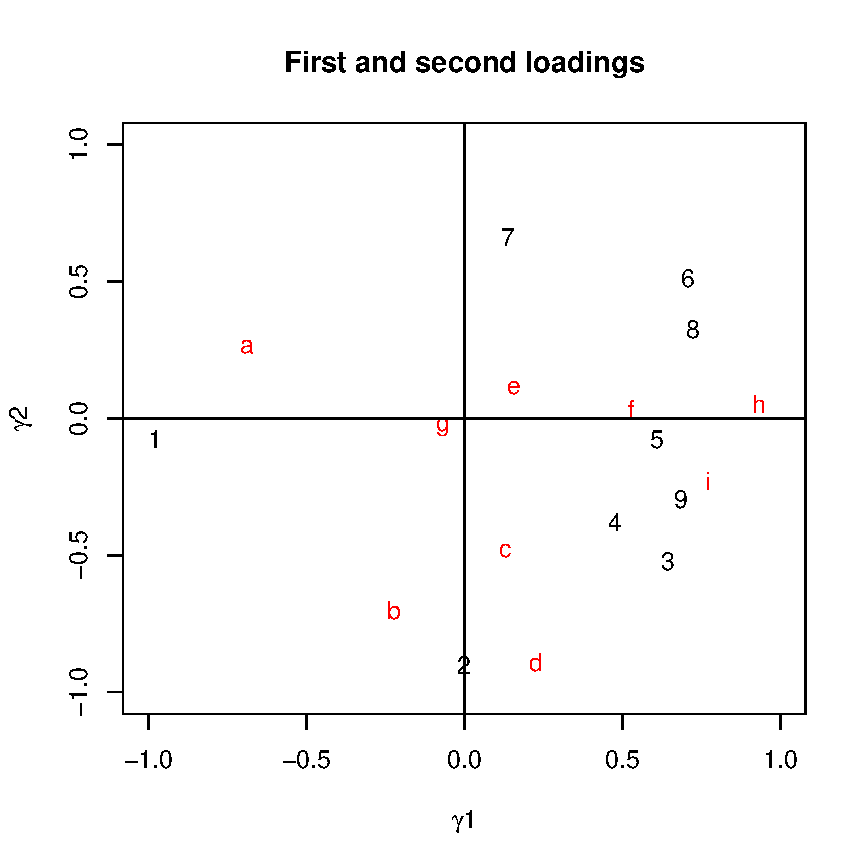
\includegraphics[width = 0.5\textwidth]{images/farotation}
\caption{Plot overlaying the co-ordinates of factor loadings 1 and 2 before and after rotation optimised by the varimax criterion}
\label{farotation}
\end{center}
\end{figure}

Although is is more difficult to see what is going on with $q=4$, we can see for example that the eighth variable (Social and Personal Services) has in increased loading in terms of $\gamma_{18}$, and a much decreased loading in terms of the second factor ($\gamma_{28}$ is virtually zero.   Thus we may feel that we have achieved some simplification of our factor structure.

\section{Factor scoring}

Finally, there are occasions where we may wish to estimate values for $\boldsymbol{\phi}_{i}$ for a given individual $i$.   These values are referred to as the scores, the process of estimating them, which has to be carried out after $\boldsymbol{\Gamma}$ and $\boldsymbol{\psi}$ have been estimated is therefore referred to as scoring.

Two methods are available in R for scoring, Thomson and Bartlett's.   The default is that no scoring takes place (it requires a data matrix).   By including \texttt{scores = "Bartlett")} or \texttt{scores = "regression"} these estimates are obtained.

\cite{Bartlett:1937,Bartlett:1938} propsed a method based upon weighted least squares.

Once we have estimates


\begin{eqnarray*}
x_{1} - \bar{x}_{1}  &=& \sum_{k=1}^{q} \hat{\gamma}_{1k} \phi_{1}  + \zeta_{1}\\
x_{2} - \bar{x}_{2} &=&  \sum_{k=1}^{q} \hat{\gamma}_{2k} \phi_{2}  + \zeta_{2}\\
&\vdots&\\
x_{p} - \bar{x}_{p} &=& \sum_{k=1}^{q} \hat{\gamma}_{pk} \phi_{p}  + \zeta_{p}
\end{eqnarray*}

we need to estimate $\phi_{j}$ for $j=1, \ldots, q$, however as $var(\zeta_{j}) = \psi_{j} $ are not equal he argued that weighted least squares was the most appropriate technique.

The weighted least squares estimates thus obtained are:

\begin{equation}
\boldsymbol{\hat{\phi}}_{i} = (\boldsymbol{\Gamma}^{T} \boldsymbol{\Psi}^{-1} \boldsymbol{\Gamma})\boldsymbol{\Gamma}^{T} \boldsymbol{\Psi}(\boldsymbol{x}_{i} - \boldsymbol{\bar{x}})
\end{equation}

\cite{Thomson:1951} is based on assuming that both $\boldsymbol{\phi}$ and $\boldsymbol{\zeta}$ are multivariate normal, thus a concatenation of the manifest ($\boldsymbol{x}$) and latent ( $\boldsymbol{\phi}$) variables $\boldsymbol{y}^{T} = (\boldsymbol{\phi}^{T}, \boldsymbol{x}^{T})$ will also be normal with dispersion matrix:

\begin{displaymath}
var(\boldsymbol{y}) = \left( \begin{array}{cc} \boldsymbol{I} & \boldsymbol{\Gamma}^{T} \\
\boldsymbol{\Gamma} & \boldsymbol{\Gamma} \boldsymbol{\Gamma}^{T} + \boldsymbol{\psi} \end{array} \right)
\end{displaymath}


The mean of $\boldsymbol{\phi}$ is zero by definition, therefore:

\begin{displaymath}
E(\boldsymbol{z} | \boldsymbol{x}_{0}) =  \boldsymbol{\Gamma}^{T}(\boldsymbol{\Gamma})\boldsymbol{\Gamma}^{T} + \boldsymbol{\Psi})^{-1}(\boldsymbol{x}_{o} - \boldsymbol{\mu})
\end{displaymath}

which gives the estimate for the scores as:

\begin{equation}
\boldsymbol{z} =  \boldsymbol{\hat{\Gamma}}^{T}(\boldsymbol{\hat{\Gamma}})\boldsymbol{\hat{\Gamma}}^{T} + \boldsymbol{\hat{\psi}})^{-1}(\boldsymbol{x}_{i} - \boldsymbol{\hat{mu}})
\end{equation}

It might be clear that factor scoring takes no account of uncertainty in the estimates of $\boldsymbol{\hat{\Gamma}}$ and $ \boldsymbol{\hat{\psi}}$, this is one area where Bayesian methods are coming to the fore \citep{Aitkin+Aitkin:2005}


%As stated, Factor Analysis is very common in application areas such as Psychometrics.   The canonical example is an analysis of intelligence testing.  We will use an example from Smith, G. A. and Stanley G. (1983) ``Clocking g: relating intelligence and measures of timed performance''. Intelligence, 7, 353-368 (presented in Bartholomew, 1990).   If we load up the \texttt{ability.cov} object we have a covariance matrix arising from six tests given to 112 individuals.   The six tests are general: a non-verbal measure of general intelligence using Cattell's culture-fair test, picture: a picture-completion test, blocks: block design, maze: mazes, reading: reading comprehension and finally vocab: vocabulary.   The underlying theory is that there exists some kind of ``general intelligence'' ($g$); the more $g$ an individual has the higher they will tend to score in all of the six tests. 

%The following code will fit a Factor Analysis model by maximum likelihood to this covariance matrix; a set of calls to \texttt{update} will increase the number of latent variables to two, and will also fit different rotations.   Part of the rationale for carrying out the rotations is to produce more readily interpreted factors.   In the case of promax, the rotation yields a number of loadings which are essentially zero.

%Bartholomew gives both covariance and correlation matrices, but these are inconsistent. Neither are in the original paper. 

%Barthlomew, D. J. (1987) Latent Variable Analysis and Factor Analysis. Griffin. 
%Barthlomew, D. J. and Knott, M. (1990) Latent Variable Analysis and Factor Analysis. Second Edition, Arnold. 


%\singlespacing
%\begin{verbatim}
%> ability.cov ## have a look at the covariance matrix
%> ?ability.cov ## get some details on the ``data''
%> ability.FA <- factanal(factors = 1, covmat=ability.cov, rotation = "none")
%> ability.FA ## have a look at the first model
%> update(ability.FA, factors=2) ## what about two latent variables
%> update(ability.FA, factors=2, rotation="varimax")
%> update(ability.FA, factors=2, rotation="promax")
%\end{verbatim}
%\onehalfspacing

%\textit{How do you interpret the various models?}   Most of our work in factor analysis will be considered with rotation and reificaton (interpreting the hidden variables).

%%% Local Variables: ***
%%% mode:latex ***
%%% TeX-master: "../book.tex"  ***
%%% End: ***



\chapter{Contemporary topics in latent variable models}
\label{latentvar}

.   Structural equation models, 
Bayesian factor analysis, sparsity priors


\chapter{Discriminant analysis}
\label{discriminant}

Discriminant analysis presupposes that we have a number of known groups of individuals, and a set of data which has been collected on individuals within these groups.   We wish to find a way of using that data to predict which group these individuals belong to, either to understand the differences or to be able to predict group membership.  \cite{Bumpus:1898} collected data on sparrows who survived and didn't survive a storm, these data are extensively analysed in this context by Manly, the primary aim of the analysis being to look for differences between the groups.   Are there different features which help us tell storm survivors from non-survivors?   More usually, we may be interested in predicting group membership.   Common examples can be found in finance; can banks tell good credit risks from bad based on data collected on customers who have subsequently defaulted on loans, see \cite{Johnson+Wichern:2002} for more details.   Another good account of discriminant analysis is given by \cite{Flury:1997} who suuggests it may be valuable when we have to carry out destructive procedures to determine group membership (such as in certain quality control investigations).  Finally a rather brief account is given in \cite{Venables+Ripley:2002}, which gives the example of disease diagnosis.   Consider a set of measurements of patient characterstics, and information determined on whether these patients have breast cancer or not.   We would be very interested in being able to make a determination of breast cancer based on the data, rather than having to wait for biopsy or other pathological information.

Discriminant analysis in one dimension seems straightforward enough.   We can examine the densities of the two groups and find an optimal cut-off point, which classifies the two groups as accurately as possible.   Some idea of the procedure is given in figure \ref{discrim}, which illustrates the idea behind discriminant function.

\begin{figure}
\begin{center}
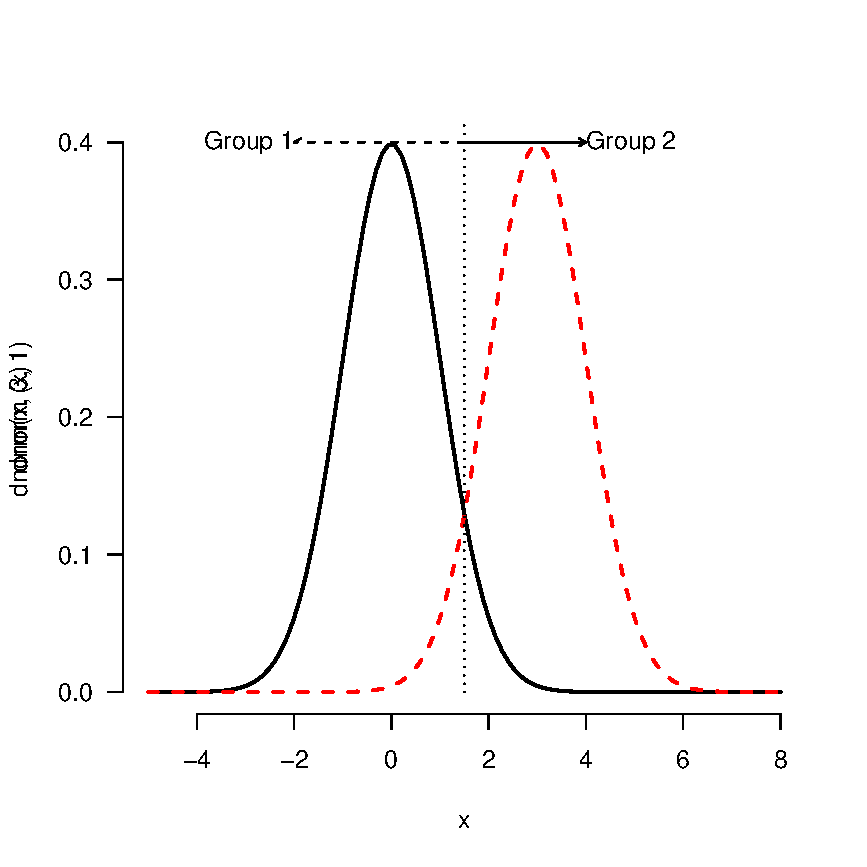
\includegraphics[width = 0.5\textwidth]{images/discrim}
\caption{Idealised discrimant function}
\label{discrim}
\end{center}
\end{figure}

Note immediately that there is a measureable risk of misclassification, which depends on the variance within groups and the separation between groups.   All we need to do is extent this procedure to work in more than one dimension.   We are going to realise this by seeking a linear combination giving us the largest separation between groups.   In other words, we are going to find linear combinations based on the original variables:

\begin{equation}
z = a_{1} x_{1} + a_{2} x_{2} + \ldots + a_{p} x_{p}
\end{equation}


However our linear combination this time will be optimised to give us the greatest potential for distinguishing the two groups.   Having found a suitable linear combination, we select a cut-off point (denoted by the vertical dotted line in the figure above), and assign observations to group 1 or group 2 based on the value relative to the cut-off.   You can see from the stylised function shown that some observations will be misclassfied!   We check the performance of this aspect of our procedure by means of a confusion matrix.


Recall that when conducting the $T^{2}$ test we essentially looked for linear combination of variables which maximised the difference between groups.   Similar ideas apply in discriminant analysis.   We seek a transformation of the data which gives the maximum ratio of group means to group variance within the two groups, i.e. we are maximising the between group variation relative to the within group variance - this should sound vaguely like what goes on in ANOVA:


\begin{tabular}{llll}
Source & d.f. & Mean Square & F ratio \\
\hline
Between groups & $m-1$ & $M_{B}$ $M_{B} / M_{W}$\\
Within groups & $N-m$ & $M_{W}$ & \\
 & N-1 & & \\
\end{tabular}

We need to find a linear combination that yields as large an F ratio as possible, hence the coefficients $a_{1}, \ldots, a_{p}$ need to be chosen to maximise this value.   More than one discriminant function is available, there are

\begin{equation}
s = min(p, m-1)
\end{equation}
discriminant functions available, where $p$ is the number of variables, and $m$ is the number of groups.

Considering the case where we have $m > 2$ groups, and $p > 2$ variables, we are looking for the following discriminant functions:


\begin{eqnarray*}
z_{1} &=& a_{11}x_{1} + a_{12}x_{2} + \ldots + a_{1p}x_{p}\\
z_{2} &=& a_{21}x_{1} + a_{22}x_{2} + \ldots + a_{2p}x_{p}\\
\ldots\\
z_{s} &=& a_{s1}x_{1} + a_{s2}x_{2} + \ldots + a_{sp}x_{p}
\end{eqnarray*}

although hopefully only  a small number of these linear combinations will account for all important differences between groups.

\section{Fisher discimination}
%\section{Fisher, linear and quadratic discimination}
\label{fisherdisc}

Remember the $T^{2}$ statistic:

\begin{equation}
T^{2}(\boldsymbol{a}) = \frac{ \left( \boldsymbol{a} (\boldsymbol{\bar{x}}_{1} - \boldsymbol{\bar{x}}_{2} ) \right)^{2} n_{1}n_{2}/(n_{1}+n_{2})}{\boldsymbol{a}^{T}\boldsymbol{S}\boldsymbol{a}}
\end{equation}

This is equivalent to finding $\boldsymbol{a}$ which maximises $|\boldsymbol{a} (\boldsymbol{\bar{x}}_{1} - \boldsymbol{\bar{x}}_{2} ) |$ subject to $\boldsymbol{a}^{T}\boldsymbol{S}\boldsymbol{a}$ = 1.   This has a single solution:

\begin{displaymath}
\boldsymbol{a} = \boldsymbol{S}^{-1}(\boldsymbol{\bar{x}}_{1} - \boldsymbol{\bar{x}}_{2} )
\end{displaymath}

and so the linear discriminant function is given by:

\begin{displaymath}
z = (\boldsymbol{\bar{x}}_{1} - \boldsymbol{\bar{x}}_{2} )^{T}\boldsymbol{S}^{-1} \boldsymbol{x}
\end{displaymath}

In two dimensions, an obvious cut-off would be the midpoint between the mean value of $z$ for group 1 and 2.


Fisher's approach has been extended to cope with more than two groups.  Again, we wish to find a linear combination $z = \boldsymbol{a}^{T} \boldsymbol{x}$ which maximised the ratio of between group variance to within group variance.

If we calculate the within sample matrix of sum of squares and cross products $\boldsymbol{W}$, and the total sample matrix of sum of squares and cross products $\boldsymbol{T}$, we can easily find the between-groups sample matrix sum of squares and cross products:

\begin{equation}
\boldsymbol{B} = \boldsymbol{T} - \boldsymbol{W}
\end{equation}



In effect we wish to maximise:

\begin{equation}
\frac{ \boldsymbol{a}^{T} \boldsymbol{B} \boldsymbol{a}}{ \boldsymbol{a}^{T} \boldsymbol{W} \boldsymbol{a}} 
\end{equation}
and usually do this subject to the condition that $\boldsymbol{a}^{T} \boldsymbol{W} \boldsymbol{a}$ = 1.   Fisher's method of discriminant analysis reduces to finding the eigenvalues and corresponding eigenvectors of $\boldsymbol{W}^{-1}\boldsymbol{B}$.   The ordered eigenvalues $\lambda_{1}, \ldots, \lambda_{s}$ are the ratio of between groups to within groups sum of squares and cross products for $z_{1}, \ldots, z_{s}$, the corresponding eigenvectors, $\boldsymbol{a}_{1}, \ldots, \boldsymbol{a}_{s}$, where $\boldsymbol{a}_{i} = \left( \begin{array}{c} a_{i1} \\ \vdots \\ a_{ip} \end{array} \right)$ are the coefficients of $z_{i}$.

We make a number of big assumptions in discriminant analysis: that observations are a random sample, that they are normally distributed and that the variance is the same for each group.   Discriminant analysis is relatively resistant to some departures from the normality assumption - it can cope with skewness but not with outliers.   %Some transformation of the data may be necessary in this situation.   It is also possible to use prior information to deal with unequal sample sizes.



%\begin{displaymath}
%W = \frac{ (\boldsymbol{X} - \boldsymbol{C} \boldsymbol{\bar{X}_{Class}})^{T} (\boldsymbol{X} - \boldsymbol{C} \boldsymbol{\bar{X}_{Class}})}{n-c}
%\end{displaymath} 

%\begin{displaymath}
%B  = \frac{  (\boldsymbol{C \bar{X}_{Class}} - \boldsymbol{I \bar{X}})^{T}(\boldsymbol{C \bar{X}_{Class}} - \boldsymbol{I \bar{X}})}{c-1}
%\end{displaymath} 

%where $\boldsymbol{\bar{X}_{Class}}$ are the mean values in a group denoted by $\boldsymbol{C}$, and $\boldsymbol{\bar{X}}$ are the overall means for data matrix $\boldsymbol{X}$.   $n$ denotes the number of individuals observed, $c$ the number of classes.



%\begin{displaymath}
%z = \alpha_{1} x_{1} + \alpha_{2} x_{2} + \ldots + \alpha_{p} x_{p}
%\end{displaymath}




%In principle, we need to carry out an eigen decomposition of the matrix $\boldsymbol{W^{-1}B}$ (although in modern computational practice a lot of the details are different, for example some rescaling goes on so that the within-group covariance is set to be $\boldsymbol{I}$).   The linear combination obtained are referred to by Manly as the canonical discriminant functions.   These linear combinations have within group variance $\boldsymbol{a^{T} W a}$ and between group variance  $\boldsymbol{a}^{T} \boldsymbol{B a}$, with the total variance given by:

%\begin{displaymath}
%\boldsymbol{a}^{T} \boldsymbol{S a}  = \frac{(n - g) \boldsymbol{W} + (g - 1) \boldsymbol{B}}{n - 1}
%\end{displaymath}





\section{Accuracy of discrimination}  
\label{accuracy}

Clearly, one important measure of the success of our discriminant rule is the accuracy of group prediction: note that there are a number of ways of measuring this and that discriminant analysis is one technique among many used in \emph{supervised classification}.   There are many techniques in machine learning and other areas which are used for classification, for example you have already met the technique of logistic discrimination.   

Model over-fitting is a known problem: we can fit a classifier really really well to our existing data but it doesn't work well next time we carry out a data collection exercise.   A key concept in this regard is the use of training and testing sets, where we split our data into two groups, and use one part to build a classifier, and the other to test it.   There are many other technques which can help in this regard, for example leave one out (loo) cross validation and some of the more recent multivariate texts should be consulted.

An important idea in terms of measuring the success of our classifier is the \emph{confusion matrix}.   This sounds rather grand, but is basically a matrix telling us how many times our discriminant function made a correct classification, and how many times it got it wrong.

\section{Importance of variables in discrimination}
\label{imporvar}

Some textbooks refer to questions surrounding selection of variables for use in a classifier.   It is important to consider whether variables are necessary for classification; often a tolerance test may be used prior to the analysis to remove multicollinear and singular variables.   It may even be desirable to carry out a dimension reducing technique.   The reason for carrying out these tests are related to over-fitting.

Some software provides ``standardised'' coefficients, the idea being that perhaps it is safe to remove variables with small standardised coefficients.   However, another approach could well be to consider classifiers with different numbers and combinations of variables and contrast the confusion matrix.   This might help identify variables which do the best job of distinguishing the groups, and those which are the least necessary.

%If $D^{2}$ is large if the discriminant function performs well.   
%Wilks' $\Lambda$ is used to assess the importance of variables: the smaller it is the more important the variable is (there are associated F statistics and p values to help in this regard).

\section{Canonical discriminant functions}
\label{candisc}

As mentioned earlier, we can have more than one discriminant function.   It is usual to plot these on a scatterplot in an attempt to visualise the discriminant ability.   However, there are tests of significance.

For example, we wish to find discriminants with a small Wilk's lambda ($\frac{|\boldsymbol{W}|}{|\boldsymbol{T}|}$), in our case this can be derived as :

\begin{equation}
\Lambda^{2} = \left( \sum_{k=1}^{m} n_{k} - 1 - \frac{1}{2}(p + m) \right) \ln (1 + \lambda_{j}),
\end{equation}
which has a $\chi^{2}$ distribution with $p + m - 2j$ degrees of freedom.


%\section{Logistic discrimination}
%\label{logdisc}

%\section{Dimension reduction and discriminant analysis}
%\label{drdisc}







\section{Linear discrimination - a worked example}

In practice, we're going to consider a classification exercise on the Iris data.   This is rather well known data featuring three species of Iris, and four anatomical measures.   First of all we need to load the \texttt{MASS} to obtain the \texttt{lda()} function.   Then we are going to pull out a training set from the Iris data.

\singlespacing
\begin{verbatim}
> library(MASS)
>  data(iris3)
>  Iris <- data.frame(rbind(iris3[,,1], iris3[,,2], iris3[,,3]),
+                         Sp = rep(c("s","c","v"), rep(50,3)))
>      train <- sample(1:150, 75)
\end{verbatim}
\onehalfspacing

\texttt{train} is a set of index numbers which will allow us to extract a training set.   We use \texttt{lda()} to fit a discriminant analysis, setting all priors equal to 1 (i.e. group memberships the same), and \texttt{subset = train} to fit the analysis to the training set.   The squiggle dot indicates that we wish to use all other variables within Iris to predict Species (Sp).

\begin{verbatim}
> z <- lda(Sp ~ ., Iris, prior = c(1,1,1)/3, subset = train)
> z
\end{verbatim}


Having extracted a training set, we are going to classify the remaining Iris' and see how well the predicted and actual species line up.

\singlespacing
\begin{verbatim}
> actual <-  Iris[-train,]$Sp
> preds <- predict(z, Iris[-train, ])$class)
> xtabs(~actual + preds)
\end{verbatim}
\onehalfspacing


One little thing to watch when using software is that in practice, Fisher's approach tends not to be used.   An approach based on probability distributions and using Bayes rule is common.   All this does, is correct for the proportions in each group to start with.   Instead of finding a discriminant rule assuming a 50:50 split, we use information on more plausible group numbers.

%%% Local Variables: ***
%%% mode:latex ***
%%% TeX-master: "../book.tex"  ***
%%% End: *** 



\chapter{Cluster analysis}
\label{clustan}

Cluster ``analysis'' describes a range of algorithms for investigating structure in data, the main interest is in finding groups of objects who are more alike.  A large number of books are dedicated to this one subject, for example \cite{Kaufman+Rousseeuw:1989,Everitt+etal:2001,Gordon:1999}, the former book supporting some rather interesting code that has been ported to \R (the S-PLUS version is described in  \cite{Struyf+etal:1997}).   It may be worth noting that some multivariate authors do not cover it at all \cite{Flury:1997} preferring a formulation based upon mixture models, and [page 316] \cite{Venables+Ripley:2002} indicate a preference for using visualisation methods for finding such structure in data.  Whilst cluster analysis is most often directed towards finding subsets of individuals that are more alike than other subsets, it is worth noting that variable clustering is also possible.   The heatmap in figure \ref{heatmap} has a dendrogram for both individuals and variables.

\singlespacing
\begin{verbatim}
x  <- as.matrix(mtcars)
rc <- rainbow(nrow(x), start=0, end=.3)
cc <- rainbow(ncol(x), start=0, end=.3)
hv <- heatmap(x, col = cm.colors(256), scale="column",
     RowSideColors = rc, ColSideColors = cc, margin=c(5,10),
     xlab = "specification variables", ylab= "Car Models",
     main = "Heatmap of mtcars data")
\end{verbatim}
\onehalfspacing

\begin{figure}
\begin{center}
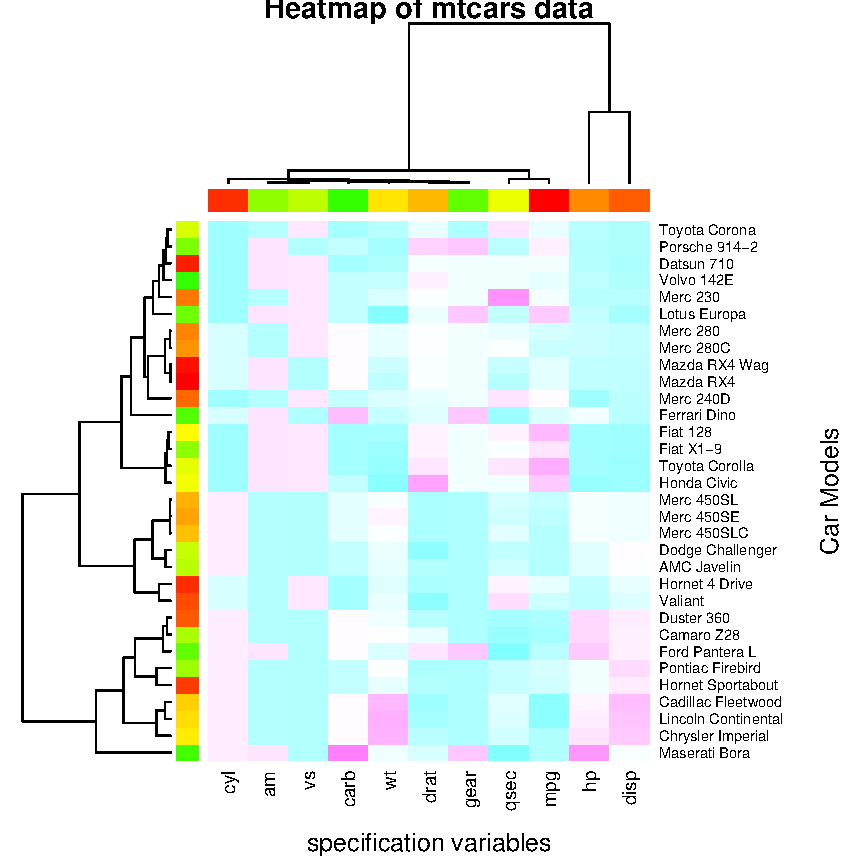
\includegraphics[width = 0.7\textwidth]{images/heatmap}
\caption{Heatmap of \texttt{mtcars} data; variables scaled in columns}
\label{heatmap}
\end{center}
\end{figure}

Modern computing facilities have widened the possibilities for visualisation considerable (both in terms of linked displays as well as the ability to numerically optimise various projection criteria).   However, when investigating the results of any scaling or projection methods there may still be interesting structures within the data.   The interest in cluster analysis lies in finding groups within the data.   When the objects within a group are very similar this can be described as internal cohesion (or homogeneity), when they is a large dissimilarity between groups this can be referred to as external separation (or isolation).   Where we have internal cohesion and external separation, one usually refers to the situation as ``clustering''. If the objects have been more-or-less
aribtrarily divided into groups we could refer to this as ``dissection''.
Clustering and dissection may both the useful in different
contexts (e.g. taxonomy and market research).   One attempt to illustrate this concept is given in figure \ref{partclust}.

%par(mfrow = c(1,2))

%x <- rbind(mvrnorm(20, c(0,-1), sigma), mvrnorm(20, c(5,4), sigma), mvrnorm(20, c(-5,4), sigma))
%plot(x, pch = 16, main = "Clustering", xlab = expression(x[1]), ylab = expression(x[2]) )
%lines(c(0,-6), c(4,-2))
%lines(c(0,0), c(4,7))
%lines(c(0,6), c(4,-1.4))
 
%x <- mvrnorm(60, c(0,4), sigma)
%plot(x, pch = 16, main = "Partitioning", xlab = expression(x[1]), ylab = expression(x[2]) )
%lines(c(0,-6), c(4,-2))
%lines(c(0,0), c(4,7))
%lines(c(0,6), c(4,-1.4))


\begin{figure}
\begin{center}
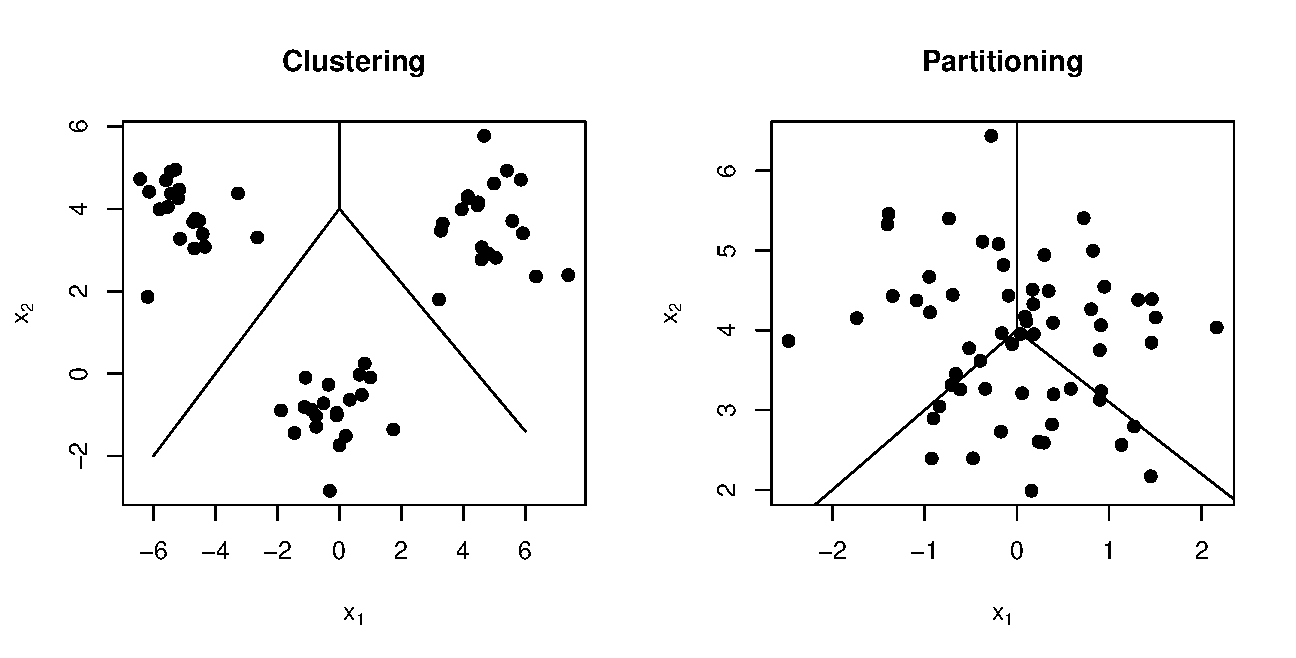
\includegraphics[width = 0.7\textwidth]{images/partclust}
\caption{Artificial data suggesting a difference between ``clustering'' and ``dissecting''}
\label{partclust}
\end{center}
\end{figure}


There are a wide range of algorithms that have been developed to investigate clustering within data.   These can be considered in a number of ways:

\begin{itemize}
\item Hierarchical Methods
  \begin{itemize}
  \item Agglomerative clustering (\verb+hclust()+, \verb+agnes()+)
  \item Divisive clustering (\verb+diana()+, \verb+mona()+)
  \end{itemize}
\item Partitioning methods (\verb+kmeans()+, \verb+pam()+, \verb+clara()+)
\end{itemize}


Hierarchical clustering provides a set of clusterings, either for $k = n, \ldots, 2$ (agglomerative) or $k = 2, \ldots, l$ (divisive).   The clustering is represented in a dendrogram and can be cut at arbitrary heights to give a fixed number of clusters.   It perhaps has a logical interpretation in numerical taxonomy.  Partitioning methods usually work by assuming a pre-determined number of clusters $k$ (although it is obviously possible to explore solutions over a range of values of $k$).   As [page 379] \cite{Seber:1984} points out, the number ofways $S_{k,n}$ of partitioning $n$ objects into $k$ groups, given by:
\begin{displaymath}
S_{k,n} = \frac{1}{k!} \sum_{j=1}^{k} \left( \begin{array}{c}k \\ j \end{array} \right) (-1)^{k-j} j^{n} \approx_{n \to \infty} \frac{k^{n}}{k!}
\end{displaymath} 
is a second type Stirling number, and where $k$ is not specified we have $\sum_{k=1}^{K} S_{k,n}$ partitions.   

For $n= 50$ and $k=2$ this is in the order of $6 \times 10^{29}$

\section{Introduction to agglomerative hierarchical cluster analysis}

Hierarchical cluster analysis finds representations that obey the ultrametric inequality.

\begin{displaymath}
d(x_{ij}, x_{ik}) \leq max(d(x_{ij}, x_{il}) d(x_{il}, x_{ik}) )
\end{displaymath}

We will work through three conventional examples of cluster analysis manually before considering an \R implementation in more detail.   For the sake of the demonstations, consider the following distance matrix:

\begin{tabular}{r|ccccc}
 & a & b & c & d & e\\
\hline
a & 0  &   &   &   &\\
b & 2  & 0 &   &   &\\
c & 6  & 5 & 0 &   & \\
d & 10 & 9 & 4 & 0 &  \\
e & 9  & 8 & 5 & 3 & 0\\
\end{tabular}

Initially, each individual is put in its own cluster.   Subsequently, at each stage individuals are joined to other individuals to form clusters, and the distance measure between a units can be readjusted in some way.   Then similar clusters are joined until all individuals have been joined.

\subsection{Nearest neighbour / Single Linkage}

This can be obtained in \R using the \verb+method = "single"+ instruction in the call to \verb+hclust()+, where it suggests that this method finds ``friends of friends'' to join each cluster in a similar way to that used in minimum spanning trees.

The decision to merge groups is based on the distance of the nearest member of the group to the nearest other object.   Clearly, with a distance of 2, inviduals $a$ and $b$ are the most similar.

\begin{minipage}[c]{0.5\textwidth}
\begin{tabular}{r|ccccc}
 & $a$ & $b$ & $c$ & $d$ & $e$\\
\hline
$a$ & 0  &   &   &   &\\
$b$ & 2  & 0 &   &   &\\
$c$ & 6  & 5 & 0 &   & \\
$d$ & 10 & 9 & 4 & 0 &  \\
$e$ & 9  & 8 & 5 & 3 & 0\\
\end{tabular}
\end{minipage}
\begin{minipage}[c]{0.5\textwidth}

We therefore merge these into a cluster at level 2:

\begin{tabular}{ll}
Distance & Groups\\
\hline
0 & a b c d e\\
2 & (ab) c d e
\end{tabular}
\end{minipage}

and we now need to re-write our distance matrix, whereby:

\begin{eqnarray*}
d_{(ab)c)} = min(d_{ac},d_{bc}) = d_{bc} = 5\\
d_{(ab)d)} = min(d_{ad},d_{bd}) = d_{bd} = 9\\
d_{(ab)e)} = min(d_{ae},d_{be}) = d_{be} = 8
\end{eqnarray*}

This gives us a new distance matrix

\begin{minipage}[c]{0.5\textwidth}
\begin{tabular}{r|ccccc}
 & $(ab)$ & $c$ & $d$ & $e$\\
\hline
$(ab)$ & 0 &   &   &  \\
$c$    & 5 & 0 &   &  \\
$d$    & 9 & 4 & 0 &  \\
$e$    & 8 & 5 & 3 & 0\\
\end{tabular}
\end{minipage}
\begin{minipage}[c]{0.4\textwidth}

Now we find that the two nearest objects are $d$ and $e$, these can be merged into a cluster at height 3:

\begin{tabular}{ll}
Distance & Groups\\
\hline
0 & $a$ $b$ $c$ $d$ $e$\\
2 & $(ab)$ $c$ $d$ $e$\\
3 & $(ab)$ $c$ $(de)$
\end{tabular}
\end{minipage}

We now need to find the minimum distance from $d$ and $e$ to the other objects and reform the distance matrix:
\begin{minipage}[c]{0.5\textwidth}
\begin{tabular}{r|ccc}
 & $(ab)$ & $c$ & $(de)$\\
\hline
$(ab)$ & 0 &   &    \\
$c$    & 5 & 0 &   \\
$(de)$ & 8 & 4 & 0  \\
\end{tabular}
\end{minipage}
\begin{minipage}[c]{0.5\textwidth}

Clearly, the next merger is between $(de)$ and $c$, at a height of 4.

\begin{tabular}{ll}
Distance & Groups\\
\hline
0 & $a$ $b$ $c$ $d$ $e$\\
2 & $(ab)$ $c$ $d$ $e$\\
3 & $(ab)$ $c$ $(de)$\\
4 & $(ab)$ $(cde)$
\end{tabular}
\end{minipage}

And it is also clear that the next step will involve merging at a height of 5.

\begin{minipage}[c]{0.5\textwidth}
\begin{tabular}{ll}
Distance & Groups\\
\hline
0 & $a$ $b$ $c$ $d$ $e$\\
2 & $(ab)$ $c$ $d$ $e$\\
3 & $(ab)$ $c$ $(de)$\\
4 & $(ab)$ $(cde)$\\
5 & $(abcde)$
\end{tabular}
\end{minipage}
\begin{minipage}[c]{0.5\textwidth}
\end{minipage}

The corresponding dendrogram is illustrated in figure \ref{simpleclust}.

\subsection{Furthest neighbour / Complete linkage}

Obtained in \R using the \verb+method = "complete"+ instruction in the call to \verb+hclust()+, where it suggests that this method finds similar clusters.   Complete linkage methods tend to find similar clusters. 

Groups are merged when the furthest member of the group is close enough to the new object.

\begin{minipage}[c]{0.5\textwidth}
\begin{tabular}{r|ccccc}
 & a & b & c & d & e\\
\hline
a & 0  &   &   &   &\\
b & 2  & 0 &   &   &\\
c & 6  & 5 & 0 &   & \\
d & 10 & 9 & 4 & 0 &  \\
e & 9  & 8 & 5 & 3 & 0\\
\end{tabular}
\end{minipage}
\begin{minipage}[c]{0.5\textwidth}
Start assembling details on the distances; we start as before
\begin{tabular}{ll}
Distance & Groups\\
\hline
0 & a b c d e\\
2 & (ab) c d e
\end{tabular}
\end{minipage}

However, the reduced distance matrix will be different:

\begin{eqnarray*}
d_{(ab)c)} = max(d_{ac},d_{bc}) = d_{ac} = 6\\
d_{(ab)d)} = max(d_{ad},d_{bd}) = d_{ad} = 10\\
d_{(ab)e)} = max(d_{ae},d_{be}) = d_{ae} = 9
\end{eqnarray*}

\begin{minipage}[c]{0.5\textwidth}
\begin{tabular}{r|ccccc}
 & (ab) & c & d & e\\
\hline
(ab) & 0  &   &   &  \\
c    & 6  & 0 &   &  \\
d    & 10 & 4 & 0 &  \\
e    & 9  & 5 & 3 & 0\\
\end{tabular}
\end{minipage}
\begin{minipage}[c]{0.5\textwidth}
Although the next step will be identical (we merge $d$ and $e$ at a height of 3)

\begin{tabular}{ll}
Distance & Groups\\
\hline
0 & a b c d e\\
2 & (ab) c d e\\
3 & (ab) c (de)
\end{tabular}
\end{minipage}

We now need to find the minimum distance from $d$ and $e$ to the other objects and reform the distance matrix:

\begin{minipage}[c]{0.5\textwidth}
\begin{tabular}{r|ccc}
 & (ab) & c & (de)\\
\hline
(ab) & 0 &   &    \\
c    & 6 & 0 &   \\
(de) & 10 & 5 & 0  \\
\end{tabular}
\end{minipage}
\begin{minipage}[c]{0.5\textwidth}
Although we are still going to merge $(de)$ and $c$ note that the height is different being 5.

\begin{tabular}{ll}
Distance & Groups\\
\hline
0 & a b c d e\\
2 & (ab) c d e\\
3 & (ab) c (de)\\
5 & (ab) (cde)
\end{tabular}
\end{minipage}

\begin{minipage}[c]{0.5\textwidth}
\begin{tabular}{r|cc}
 & (ab) & (cde)\\
\hline
(ab)  & 0   &     \\
(cde) & 10 &  0  \\
\end{tabular}
\end{minipage}
\begin{minipage}[c]{0.5\textwidth}
So our final merge will take place at height 10.

\begin{tabular}{ll}
Distance & Groups\\
\hline
0 & a b c d e\\
2 & (ab) c d e\\
3 & (ab) c (de)\\
5 & (ab) (cde)\\
10 & (abcde)
\end{tabular}
\end{minipage}

In this simple demonstration, the dendrogram, illustrated in the centre of figure \ref{simpleclust} obtained is similar in shape, but all the merges are at different height.  


\subsection{Group average link}

This requires \texttt{agnes()} in package \texttt{cluster}, called with the \verb+method="average"+ instruction.

This time we merge two groups is the average distance between them is small enough.

\begin{minipage}[c]{0.5\textwidth}
\begin{tabular}{r|ccccc}
 & a & b & c & d & e\\
\hline
a & 0  &   &   &   &\\
b & 2  & 0 &   &   &\\
c & 6  & 5 & 0 &   & \\
d & 10 & 9 & 4 & 0 &  \\
e & 9  & 8 & 5 & 3 & 0\\
\end{tabular}
\end{minipage}
\begin{minipage}[c]{0.5\textwidth}
Start assembling details on the distances; again, we start as before:
\begin{tabular}{ll}
Distance & Groups\\
\hline
0 & a b c d e\\
2 & (ab) c d e
\end{tabular}
\end{minipage}

But the reduced distance matrix will be different again:

\begin{eqnarray*}
d_{(ab)c)} = (d_{ac} + d_{bc})/2  = 5.5\\
d_{(ab)d)} = (d_{ad} + d_{bd})/2  = 9.5\\
d_{(ab)e)} = (d_{ae}+ d_{be})/2  = 8.5
\end{eqnarray*}


\begin{minipage}[c]{0.5\textwidth}
\begin{tabular}{r|ccccc}
 & (ab) & c & d & e\\
\hline
(ab) & 0  &   &   &  \\
c    & 5.5  & 0 &   &  \\
d    & 9.5 & 4 & 0 &  \\
e    & 8.5  & 5 & 3 & 0\\
\end{tabular}
\end{minipage}
\begin{minipage}[c]{0.5\textwidth}
Yet again, the next merge step will be identical (we merge $d$ and $e$, only they are merged at height 3)

\begin{tabular}{ll}
Distance & Groups\\
\hline
0 & a b c d e\\
2 & (ab) c d e\\
3 & (ab) c (de)
\end{tabular}
\end{minipage}

We now need to find the minimum distance from d and e to the other objects and reform the distance matrix:

\begin{minipage}[c]{0.5\textwidth}
\begin{tabular}{r|ccc}
 & (ab) & c & (de)\\
\hline
(ab) & 0 &   &    \\
c    & 5.5 & 0 &   \\
(de) & 9 & 4.5 & 0  \\
\end{tabular}
\end{minipage}
\begin{minipage}[c]{0.5\textwidth}
Again, we still going to merge $(de)$ and $c$ note that the height is different ($4.5$)

\begin{tabular}{ll}
Distance & Groups\\
\hline
0 & a b c d e\\
2 & (ab) c d e\\
3 & (ab) c (de)\\
5 & (ab) (cde)
\end{tabular}
\end{minipage}

\begin{minipage}[c]{0.5\textwidth}
\begin{tabular}{r|cc}
 & (ab) & (cde)\\
\hline
(ab)  & 0   &     \\
(cde) & 7.8 &  0  \\
\end{tabular}
\end{minipage}
\begin{minipage}[c]{0.5\textwidth}
So our final merge will take place at height $7.8$.

\begin{tabular}{ll}
Distance & Groups\\
\hline
0 & a b c d e\\
2 & (ab) c d e\\
3 & (ab) c (de)\\
4.5 & (ab) (cde)\\
7.8 & (abcde)
\end{tabular}
\end{minipage}

In this simple demonstration, the dendrogram obtained is similar in shape, but all the merges are at different height.   This dendrogram is depicted on the right of figure \ref{simpleclust}.   Whilst the role of the dendrogram seems obvious, it should be acknowledged that there are some algorithmic details needed to determine how to present these.   We will consider other clustering methods shortly, but it should be noted that the centroid and median approaches can lead to reversals in the dendrogram.

\begin{figure}
\begin{center}
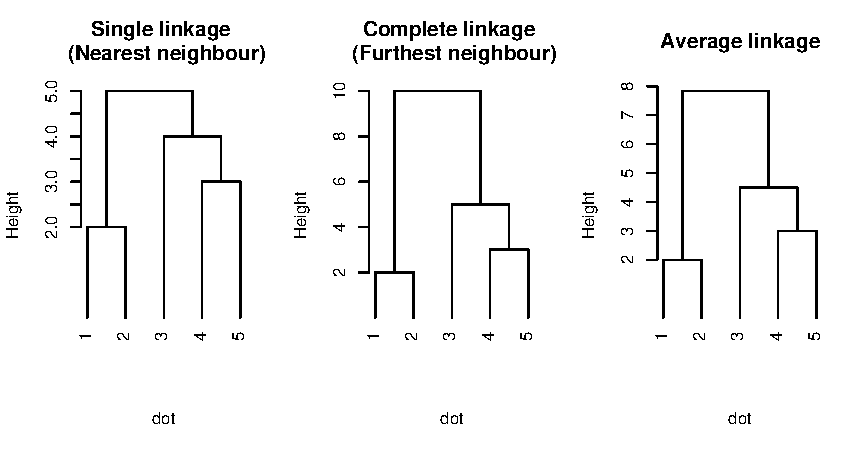
\includegraphics[width = 0.7\textwidth]{images/democlust}
\caption{Dendrograms from three basic cluster methods}
\label{simpleclust}
\end{center}
\end{figure}

%\begin{itemize}
%\item Ward's minimum variance method aims at finding compact, spherical clusters. 
%\item Complete linkage method finds similar clusters. 
%\item The single linkage method (which is closely related to the minimal spanning tree) adopts ``friends of friends'' clustering strategy. 
%\item Other methods are somewhere between single and complete link methods. 
%\end{itemize}

\subsection{Alternative methods for hierarchical cluster analysis}
\label{othermethods}

Given that cluster ``analysis'' is essentially an algorithmically guided exploratory data analysis it is perhaps no surprise, firstly that there have been many other methods proposed and secondly that there have been attempts to generalise the algorithm.   \cite{Lance+Williams:1966,Lance+Williams:1967} proposed a general recurrence formula which gives the distance between a newly amalgated group $C_{k} \bigcup C_{l}$ and some other group $C_{m}$:

\begin{equation}
d_{C_{k} \bigcup C_{l}, C_{m}} = \alpha_{l} d(C_{k}, C_{l}) + \alpha_{m} d(C_{k}, C_{m}) + \beta d(C_{k}, C_{l}) + \gamma \lvert d(C_{k}, C_{m}) -  d(C_{l}, C_{m})\rvert 
\end{equation}
where $d_{C_{k} \bigcup C_{l}, C_{m}}$ is the distance between a cluster $C_{k}$ and the merging of two groups  $C_{l}$ and $C_{m}$.   The parameters are constrained such that $\alpha_{l} + \alpha_{m} + \beta = 1$, $\alpha_{l} = \alpha_{m}$, $\beta < 1$ and $\gamma = 0$.   Using these schema, a number of established agglomerative strategies can be expressed as follows:
\begin{tabular}{lrrrr}
Method & \R call &  $\alpha_{k}$ & $\beta$ & $\gamma$ \\
\hline
Single link (nearest neighbour) & \verb+method = "single"+ & $\frac{1}{2}$ & 0 & $-\frac{1}{2}$ \\
Complete link (furthest neighbour) &  \verb+method = "complete"+ & $\frac{1}{2}$ & 0 & $\frac{1}{2}$ \\
Group average link &  \verb+method = "average"+ & $N_{l}|(N_{l} + N_{m})$ & 0 & 0\\
Weighted average link &  \verb+method = "mcquitty"+ & $\frac{1}{2}$ & 0 & 0 \\
Centroid &   \verb+method = "centroid"+ & $N_{l}|(N_{l} + N_{m})$ &  $- N_{l} N_{m}|(N_{l} + N_{m})^2$ & 0\\
%Sum of squares &  \verb+method = ""+ &  $(N_{i} + N_{K})|(N_{i} + N_{j} + N_{k})$ & $-(N_{K} + N_{k})|(N_{i} + N_{j} + N_{K})$
Incremental sum of squares &  \verb+method = "ward"+ & $\frac{N_{k} + N_{m}}{N_{k} + N_{l} + N_{m}}$ &  
$\frac{N_{k} + N_{l}}{N_{k} + N_{l} + N_{m}}$ & 0 \\
Median &  \verb+method = "median"+ & $\frac{1}{2}$ & $-\frac{1}{4}$ & 0\\
%Flexible & $\frac{1}{2}(1-\beta)$ & $\beta(<1)$ & 0\\
\end{tabular}
where $N_{k}, N_{l}\ \mbox{and}\ N_{m}$ are the cluster sizes when $C_{k}$ is joined to the other two clusters considered.

This formula facilitates the use of a number of clustering approaches.   \cite{Ward:1963} proposed a method in which clustering proceeds by selecting those merges which minimise the error sum of squares.   If we consider the cluster specific error sum of squares:
\begin{displaymath}
ESS_{k} = \sum_{i+1}^{n_{k}} \sum_{j=1}^{p} (x_{ki,j} - \bar{\boldsymbol{x}}_{k,j})^{2}
\end{displaymath}
where $ \bar{\boldsymbol{x}}_{k,j}$ is the mean of cluster $k$ with respect to variable $j$ and $x_{ki,j}$ is the value of $j$ for each object $i$ in cluster $k$.   The total error sum of squares is therefore given by $\sum_{k=1}^{K} ESS_{k}$ for all clusters $k$.   This method tends to give spherical clusters, whether that is a reasonable solution to find or not.

 Centroid clustering involves merging clusters with the most similar mean vectors; there is a subtle variation on a theme in which the centroid calculation is weighted.   Whilst the calculations underlying these methods tend to use Euclidean distance (to facilitate interpretation in terms of the raw data) that is not compulsory.   There is therefore some quite unsubtle interaction between choice of distance measure and choice of clustering algorithm which provides vast room for ambiguity in conducting cluster analysis.


\subsection{Problems with hierarchical cluster analysis}

A number of problems have been recognised with hierarchical cluster analysis.   Single, complete and average linkage as well as Ward's method have the potential for reversals in the dendrogram; single and complete linkage impose a monotonicity requirement.   One particular problem with single link clustering is ``chaining'', we could illustrate this as follows:
\singlespacing
\begin{verbatim}
x <- rbind(mvrnorm(30, c(0,0), sigma), 
  mvrnorm(30, c(8,8), sigma), 
  cbind(seq(0,8, by = 0.4), seq(0,8, by = 0.4) )
dot <- hclust(dist(x), method = "single")
par(mfrow = c(1,2))
plot(dot)
plot(x, pch = cutree(dot, k = 2))
\end{verbatim}
\onehalfspacing


\begin{figure}
\begin{center}
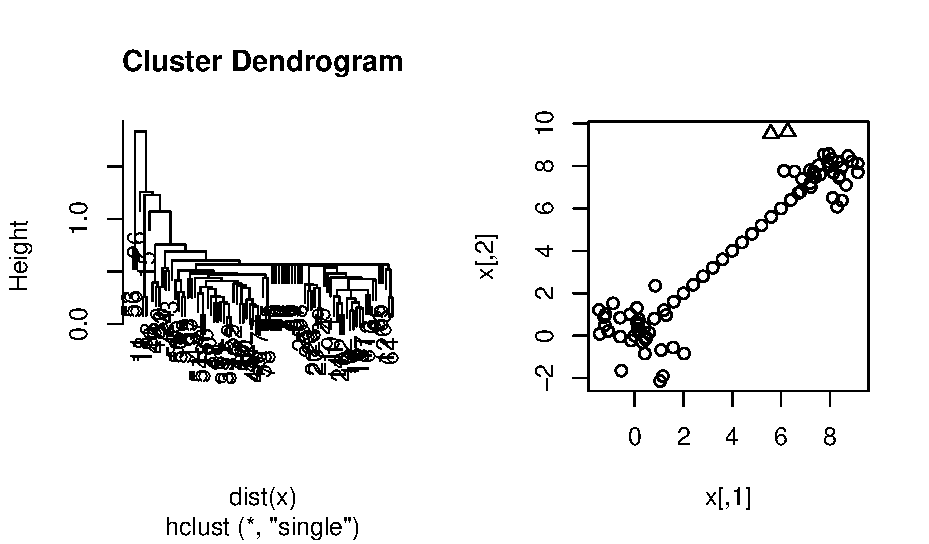
\includegraphics[width = 0.7\textwidth]{images/chaining}
\caption{Demonstration of ``chaining'' with single link clustering}
\label{chaining}
\end{center}
\end{figure}


\subsection{Hierarchical clustering in \R}

A typical example of a cluster analysis was reported by \cite{Jolliffe+etal:1986}. To carry out hierarchical cluster analysis in \R, create a distance object from the data (\verb+USArrests.dist+), create a hierarchical clustering object from the distance matrix (\verb+USArrests.hclust+), and plot the results.   Here we have used manhattan distance and compete linkage.  You may like to see how much difference the alternatives make.

\singlespacing
\begin{verbatim}
> USArrests.dist <- dist(USArrests, method = "manhattan")
> USArrests.hclust <- hclust(USArrests.dist, method = "complete")
> plot(USArrests.hclust)
\end{verbatim}
\onehalfspacing

\begin{figure}
\begin{center}
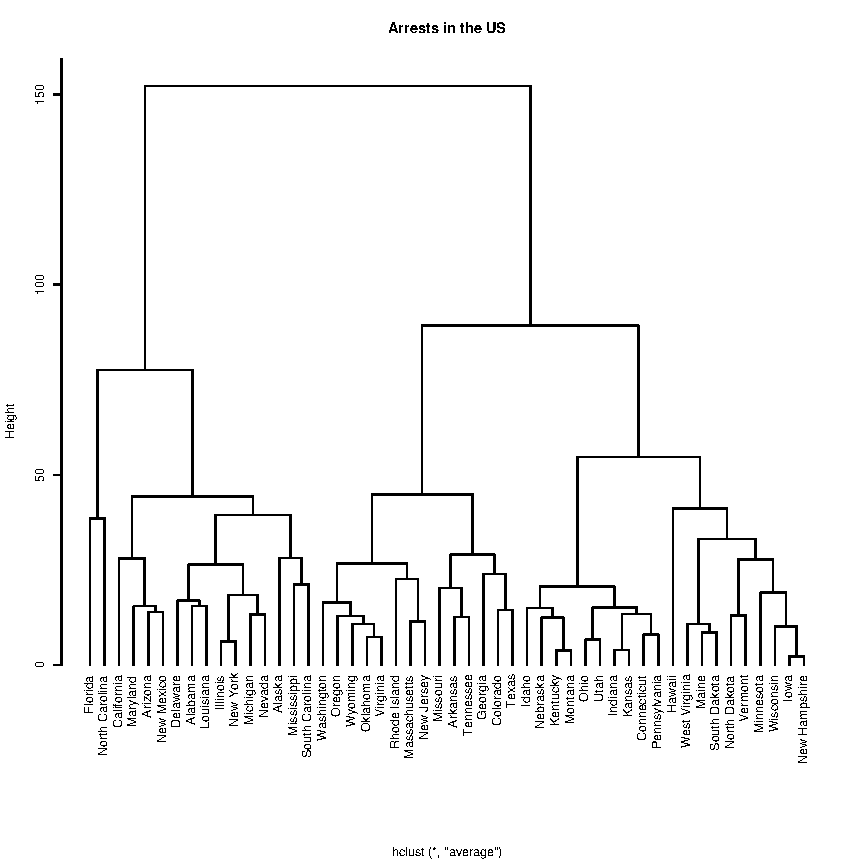
\includegraphics{images/hclust}
\caption{Dendrogram following complete linkage cluster analysis of US Arrests data}
\label{hclust}
\end{center}
\end{figure}

For comparison with other results, we may want to ``cut'' the dendrogram at a point which gives us a certain number of classes.   Here, we will cut the dendrogram fairly high up, and look at a possible five group structure.   In the following code, we use cutree to find the five groups, and produce draftsman plot with colours / symbols altering according to which of the five groups we think the state may belong to.

\singlespacing
\begin{verbatim}
> hc.class <- cutree(USArrests.hclust, k =5)
> plot(USArrests, col = hc.class, pch = hc.class)
\end{verbatim}
\onehalfspacing

An agreement is where both objects have a one in each position.   $b$ and $c$ denote the two possibly disagreements.

\section{Cophenetic Correlation}

The cophenetic correlation can be used as some kind of measure of the goodness of fit of a particular dendrogram.

\begin{equation}
\rho_{Cophenetic} = \frac{\sum_{i=1, j=1, i <j}^{n} (d_{ij} - \bar{d})(h_{ij} - \bar{h})}{
\left(\sum_{i=1, j=1, i <j}^{n} (d_{ij} - \bar{d})^{2}(h_{ij} - \bar{h})^{2} \right)^{0.5}}
\end{equation}

\singlespacing
\begin{verbatim}
> d1 <- dist(USArrests)
> h1 <- hclust(d1)
> d2 <- cophenetic(h1)
> cor(d1, d2)
[1] 0.7636926
> h1 <- hclust(d1, method = "single")
> d2 <- cophenetic(h1)
> cor(d1, d2)
[1] 0.5702505
\end{verbatim}
\onehalfspacing

So it is easy to obtain a measure of the cophenetic correlation, it is less clear what it means.   Certainly a value below 0.6 implies that there has been some distortion in the dendrogram.

\section{Divisive hierarchical clustering}
\label{aggclust}

Divisive clustering reverses the approach taken above.   Here, we start with one large cluster of all $n$ objects, and split until each object is unique. 
[page 90] \cite{Gordon:1999} argues that divisive clustering is not likely to lead to optimal divisions in the data.   Arguably the more succesful methods are monothetic and split on one variable at each stage (see \verb+mona()+ for an R example which works with binary data).      

\cite{MacNaughton-Smith+etal:1964} proposed one divisive method which has seen some use.   \cite{Kaufman+Rousseeuw:1989} liken this to splintering within a political party, where one person leaves and attracts the most like-minded people and have provided the \verb+diana()+ routine which facilitates this form of clustering.   


To identify the ``splinter'', the object with the largest average dissmilarity to all other objects is selected.   Then the dissimilarities are recalculated, and any objects who are closer to the splinter than to their original group are reclassified.   Average dissimilaries can then be recalculated.


At each subsequent step of the algorithm, the cluster $C$ with the largest diameter is selected:

\begin{displaymath}
diam(C) = max_{i,j \in C} d(i,j)
\end{displaymath}

This diameter is represented as the ``height'' in the dendrogram and the banner plot.

Then $C$ is split into two subclusters, initially $A=C$ and $B=\emptyset$.   For each objects in $A$, calculate the average dissimilarity to all other objects in $A$, the object with the largest distance is moved to $B$.   This step is repeated until there are $n$ clusters. 



\singlespacing
\begin{verbatim}
USArrests.dist <- dist(USArrests)
library(cluster)
USArrests.diana <- diana(USArrests.dist)
par(mfrow = c(1,2), oma = c(0,0,2,0))
plot(USArrests.diana, which = 2, cex = 0.6, 
main = "Dendrogram", xlab = "")
plot(USArrests.diana, which = 1, main = "Banner plot", 
nmax.lab = 50, cex.axis = 0.6, max.strlen = 12)
mtext("Divisive clustering of USArrests", outer = TRUE)
\end{verbatim}
\onehalfspacing




\begin{figure}
\begin{center}
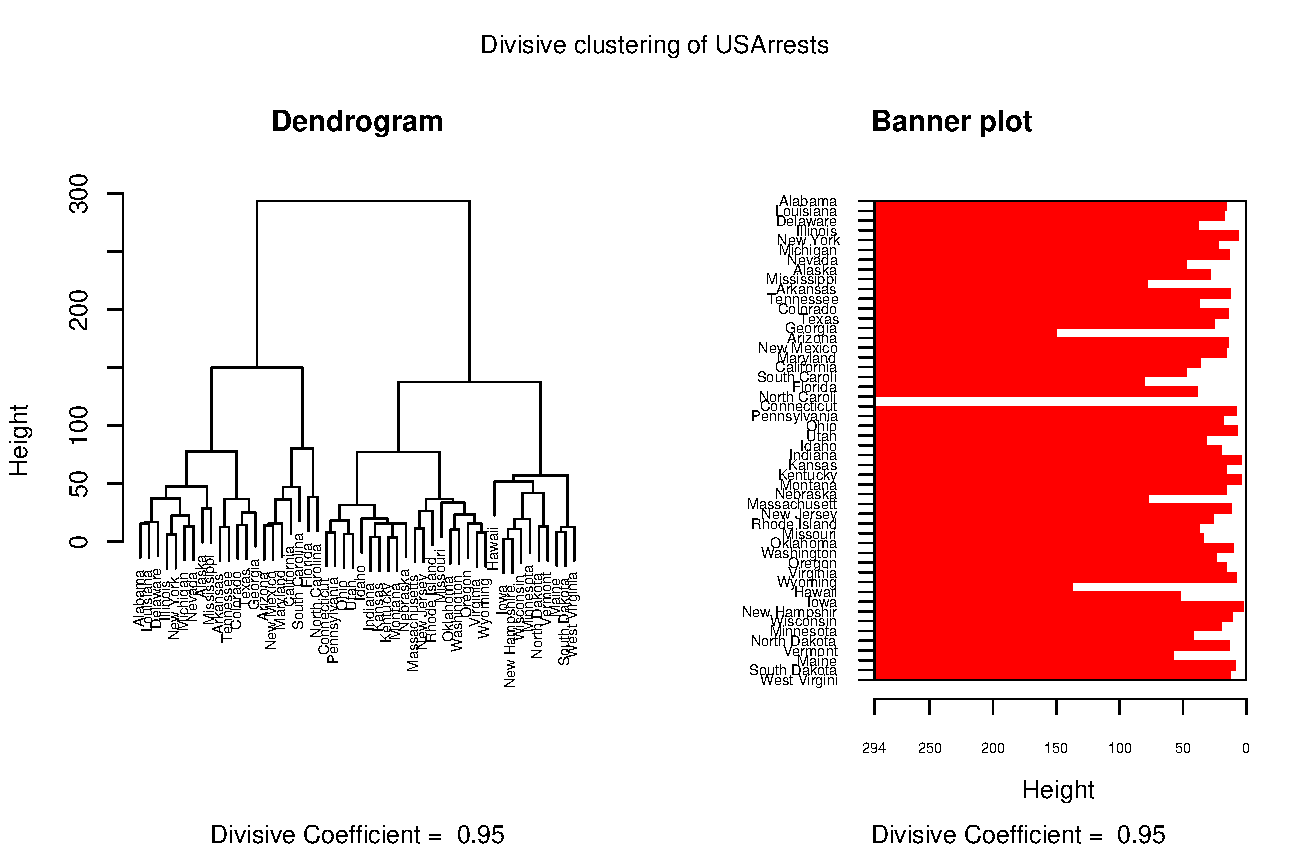
\includegraphics[width = 0.8\textwidth]{images/diana}
\caption{Divisive clustering of USArrests data, dendrogram and bannerplot}
\label{diana}
\end{center}
\end{figure}


\section{K-means clustering}
\label{kmclust}

This is a rather different method of clustering, aimed at finding ``more homogenous'' subgroups within the data.   We specify at the start how many clusters we are looking for, and ideally provide some clue as to what might be in those clusters.

The technique was perhaps first proposed by \cite{Lloyd:1957} and somewhat codified by \cite{Forgy:1965}, early developments were also reported by \cite{MacQueen:1967}, although the default S-Plus algorithm was developed by \cite{Hartigan+Wong:1979}.   There is some confusion as to whether \emph{k-means} refers to a particular technique or a particular algorithm.

Given a number of $k$ starting points, the data are classified, the centroids recalculated and the process iterates until stable.

We could attempt to demonstrate this with the following function

\singlespacing
\begin{verbatim}
step <- function(X, mu1, mu2){
## classify according to current seed point (expectation step)
one <- sqrt(rowSums((X - t(t(t(mu1)) %*% t(ones)))^2))
two <- sqrt(rowSums((X - t(t(t(mu2)) %*% t(ones)))^2))
plot(x,y, col = 1 + as.numeric(one < two), pch = 16, xlim = xlims, ylim = ylims )
legend("topright", pch = c(16,16,2,3), col = c("red", "black"), legend = c("Group1", "Group2", "Seed 1", "Seed 2" ), cex = 0.5)
points(rbind(seed$mu1, seed$mu2), pch = c(2,3), col = c("red", "black"))
fixed <- (mu1 + mu2)/2
slope <- -(mu1[1] - mu2[1])/(mu1[2] - mu2[2])
abline(c(fixed[2] - slope * fixed[1], slope))

## calculate new seed points (maximisation step)
mu1 <- colMeans(X[one < two,])
mu2 <- colMeans(X[one >= two,])
return(seed = list(mu1 = mu1, mu2 = mu2))
}
\end{verbatim}
\onehalfspacing

And set up with:

\singlespacing
\begin{verbatim}
## simulate two clusters of data
x <- c(rnorm(20,0,1), rnorm(20,4,1))
y <- c(rnorm(20,0,1), rnorm(20,4,1))
X <- cbind(x,y)
ones <- matrix(1, dim(X)[1],1)

## set up some parameters for plotting
xlims <- c(min(x), max(x)) * 1.3
ylims <- c(min(y), max(y)) * 1.3

## plot the data
par(mfrow = c(2,2))
plot(X, xlim = xlims, ylim = ylims)

## And add some very silly seed points
mu1 <- c(0,6)
mu2 <- c(5,-2)
seed <- list(mu1 = mu1, mu2 = mu2)
points(rbind(seed$mu1, seed$mu2), pch = c(2,3),col = c("red", "black"))
legend("topright", pch = c(1,2,3), col = c("black", "red", "black"), legend = c("Data", "Seed 1", "Seed 2" ), cex = 0.5)
##mtext(paste("Seed points: \n Group 1 ", formatC(seed[[1]],2), "Group 2 ", formatC(seed[[2]],2)))

seed <- step(X, seed$mu1, seed$mu2)
seed <- step(X, seed$mu1, seed$mu2)
seed <- step(X, seed$mu1, seed$mu2)
\end{verbatim}
\onehalfspacing

\begin{figure}
\begin{center}
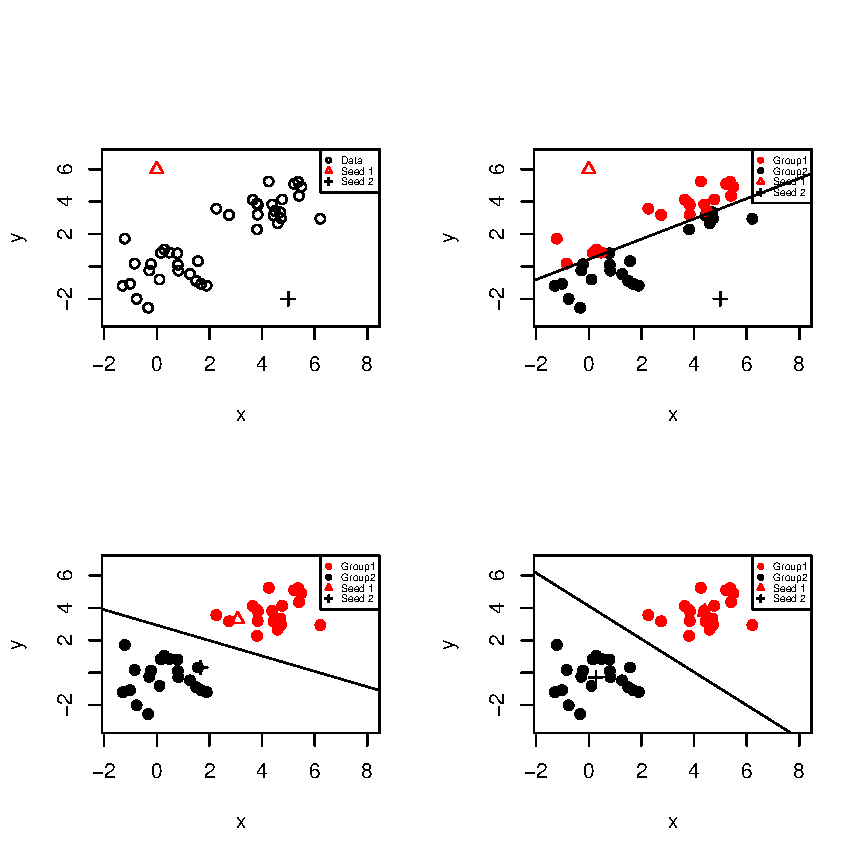
\includegraphics[width = 0.7\textwidth]{images/kmeansdemo}
\label{kmeansdemo}
\caption{Demonstration of kmeans algorithm, points are classified according to seed, then position of seed is recalculated}
\end{center}
\end{figure}

Having illustrated the basic principles it is quite easy to run the analysis:

\singlespacing
\begin{verbatim}
> US.km <- kmeans(USArrests, centers = 2)
> plot(USArrests, col = US.km$cluster, pch = US.km$cluster) ## not shown
> plot(prcomp(USArrests, center = TRUE)$x[,c(1,2)], 
col = US.km$cluster, pch = US.km$cluster)
 
\end{verbatim}
\onehalfspacing
For interest, we will compare the $k$-means solution with the \verb+diana()+ classification: 

\singlespacing
\begin{verbatim}
 kmclass <- as.vector(US.km$cluster)
> diana.class <- cutree(USArrests.diana, k = 2)
> xtabs(~kmclass + diana.class)
       diana.class
kmclass  1  2
      1  0 29
      2 21  0
\end{verbatim}
\onehalfspacing

So in this particular example, there is good agreement that there may be two clusters in the data.

\begin{figure}
\begin{center}
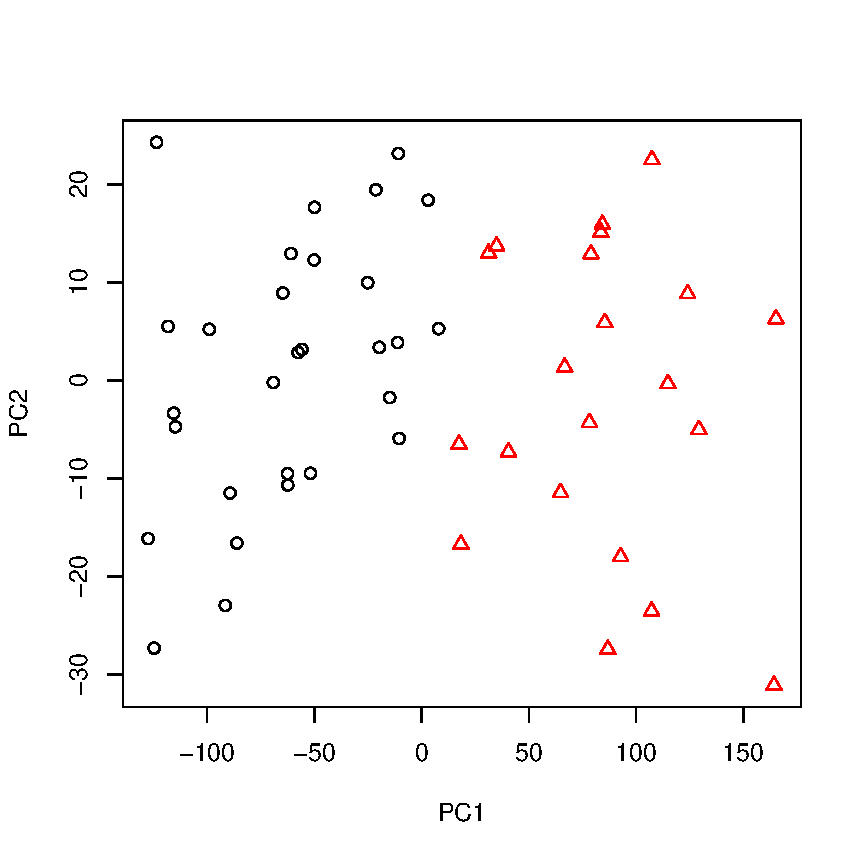
\includegraphics[width = 0.6\textwidth]{images/km2classpca}
\caption{Scatterplot of original variables denoting cluster membership for $k=2$ means clustering}
\label{hclust}
\end{center}
\end{figure}


\subsection{Partitioning around medoids}

This approach to clustering is laid out in \cite{Kaufman+Rousseeuw:1989}, and the S-PLUS implementation is very well described in \cite{Struyf+etal:1997}.   The procedure is to find $k$ \emph{representative objects} called medoids in such a way that the total dissimilarity of all objects to their nearest medoids is minimised.   One side-effect of this approach is that a data entity is identifed as a \emph{representative object} which may facilitate description rather better than a non-existing group centroid.   In other words, we identify objects that ``best'' represent their groups.   This is quite simple to do in \R, we can supply either the data matrix or a distance matrix to \verb+pam()+, below we supply the data:
\singlespacing
\begin{verbatim}
> USArrests.pam <- pam(USArrests, k = 2)
> par(mfrow = c(1,2))
> plot(USArrests.pam)
> USArrest.pam$medoids
         Murder Assault UrbanPop Rape
Michigan   12.1     255       74 35.1
Kansas      6.0     115       66 18.0
\end{verbatim}
\onehalfspacing
and it can be seen that Michigan and Kansas are in some sense the best representative examples of each of the two groups we have chosen to investigate.   The \verb+plot()+ method applied to pam objects produces a $2 \times 2$ scatterplot of the first two principal components identifying group memberships and superimposing ellipses as well as a silhouette.

\begin{figure}
\begin{center}
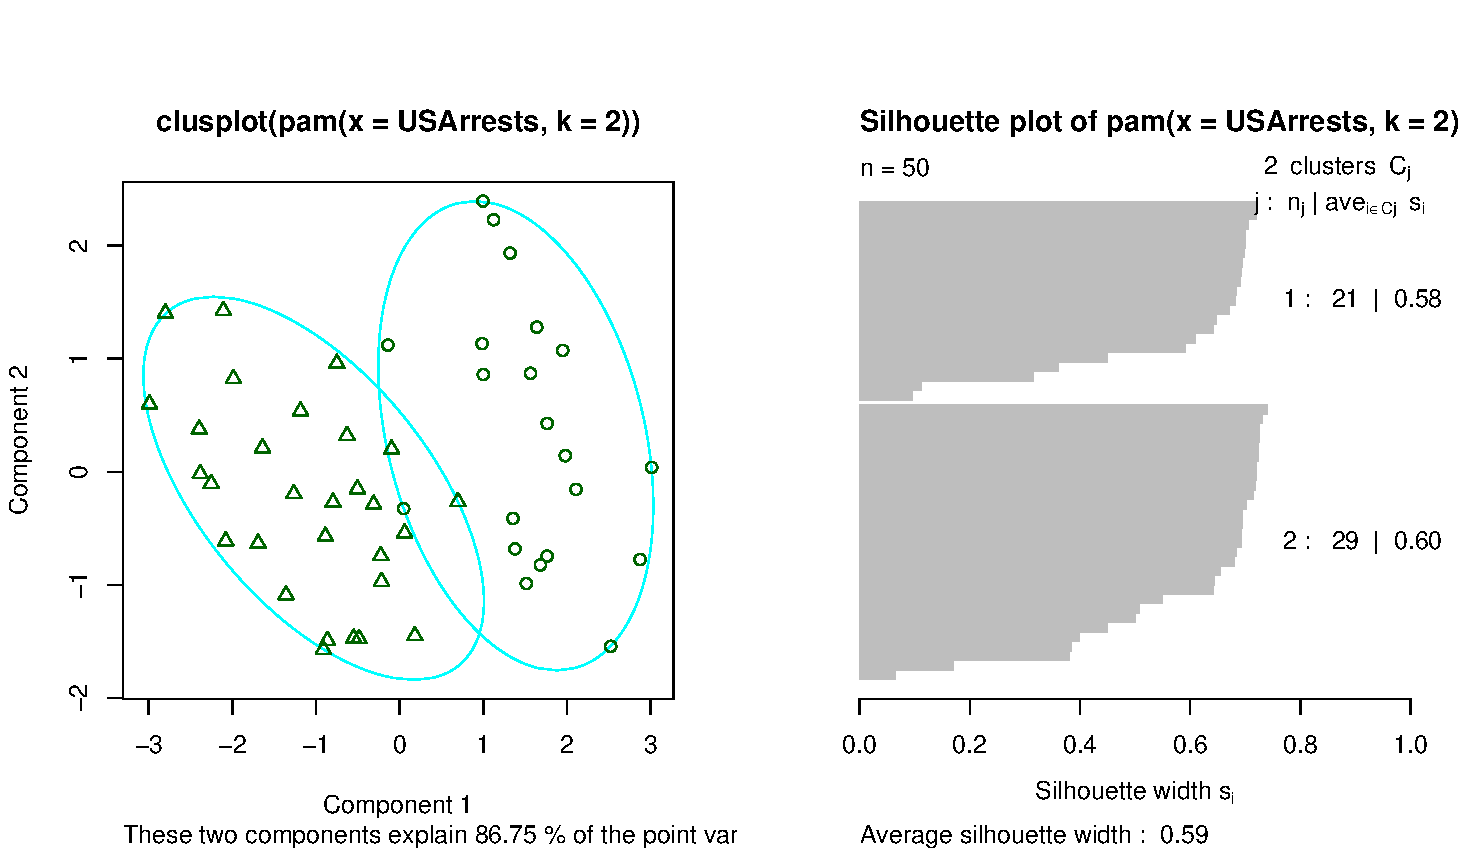
\includegraphics[width = 0.8\textwidth]{images/pam}
\caption{Partitioning around medoids}
\label{pam}
\end{center}
\end{figure}

With minor modification, this is a tractable algorithm for large datasets.   A wrapper, \verb+clara()+ has been written which makes partitioning around mediods available for a wide range of datasets.

\subsection{Hybrid Algorithms}

There have been a number of proposals in the literature recently for hybrid algrithms.   We consider HOPACH, essentially it is a divisive algorithm, but at each stage a merging step is incorporated to bring together similar clusters (which may be on different branches of the tree).  Again, this method produces medoids, in this case 13 were identified.

\singlespacing
\begin{verbatim}
> library(hopach)
> USArrests.hopach <- hopach(USArrests)
> row.names(USArrests)[USArrests.hopach$clustering$medoids]
 [1] "Mississippi"   "Alaska"        "New Mexico"    "Michigan"     
 [5] "California"    "Illinois"      "Missouri"      "West Virginia"
 [9] "Rhode Island"  "Nebraska"      "New Hampshire" "Wisconsin"    
[13] "Hawaii"     
> dplot(dist(USArrests), us, labels = row.names(USArrests), main = "HOPACH of USArrests")
\end{verbatim}
\onehalfspacing

The \verb+dplot()+ method requires input of a distnce matrix and produces a heatmap of the distances ordered by the cluster structure.   Silhouette plots are also available, and further plot methodology is available from programs external to \R.

\begin{figure}
\begin{center}
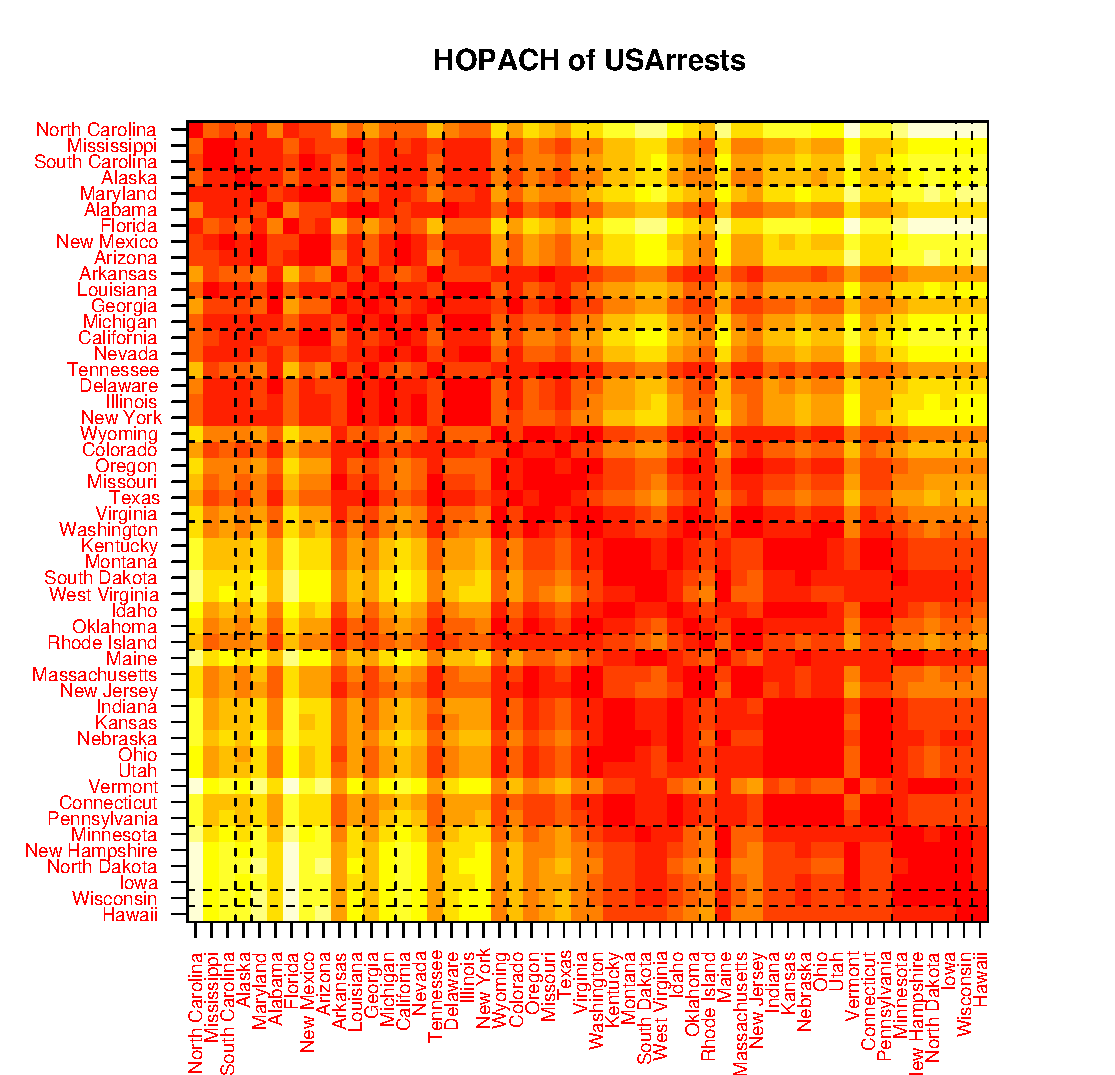
\includegraphics[width = 0.7\textwidth]{images/hopach}
\caption{Heatmap of distances organised according to output of HOPACH with cluster groups denoted by dashed lines}
\label{hopach}
\end{center}
\end{figure}

\section{K-centroids}

More recent proposals in the literature have tried to remove the dependency on algorithmic dependency.   I need to add something on this shortly.



\section{Further information}

It is worth repeating that ``cluster analysis'' is a poorly delimited set of methods for unsupervised classification.   Obvious omissions include fuzzy analysis (where we accept some uncertainty in group assignments), monothetic analysis (where we split based on binary variables one at a time).   All these merit further consideration.   However, it is acknowledged that the greatest omission at present is in terms of mixture modelling, much more comprehensive information is available in \cite{McLachlan+Peel:2000}, some coverage is also given in \cite{Flury:1997}.



%%% Local Variables: ***
%%% mode:latex ***
%%% TeX-master: "../book.tex"  ***
%%% End: ***

\chapter{Multidimensional scaling}
\label{mds}

%\section{Principal co-ordinates analysis - multidimensional scaling}


We have looked at clustering techniques which partition an $n \times n$ matrix of dissimilarities into groups of like individuals.   Whilst it is possible to visualise differences between individuals in terms of dendrograms, it might be more useful to have a direct representation of the relationship between individuals.   We are now going to consider techniques which let us visualise the relative distances bewteen individuals in a low dimensional structure.  Some early ideas were set out by \cite{Richardson:1938}, and the algebraic techniques required to reconstruct a configuration from distances were established by \cite{Young+Householder:1938}.   \cite{Torgerson:1952} set out the foundations for this work, but developments in the technique associated with the name \emph{principal co-ordinates analysis} were given by \cite{Gower:1966}.   Arguably, the tecnique is most commonly referred to as \emph{scaling}, often as classical scaling.

\section{Metric Scaling}

Consider (any) distance matrix $\boldsymbol{\Delta}$.   It is metric if elements of $\boldsymbol{\Delta}$ satisfy the metric (triangle) inequality $\delta_{ij} \leq \delta_{ik} + \delta_{kj}$ for all $i$, $j$, $k$.

Classical metric multidimensional scaling is based on the $n \times n$ distance or dissimilarity matrix, we will note later some connections with principal components.   Here, we will first consider a matrix $\boldsymbol{\Delta}$ of \emph{Euclidean} distances between objects, such that $\delta_{ij}$ is the distance between points $i$ and $j$.   These $n$ points can be represented in $n-1$ dimensional space.   We are looking for a configuration of $n$ points such that the distance $d_{ij}$ between points $i$ and $j$ equals the dissimilarity $\delta_{ij}$ for all $i$, $j$.   The dimensionality of this configuration is $q$ such that we are seeking to reconstruct an $n \times q$ matrix $\boldsymbol{X}$.

We can very easily get from an $n \times p$ matrix $\boldsymbol{X}$ to a Euclidean distance matrix.   If we first form the $n \times n$ matrix $\boldsymbol{Q}$ then $\boldsymbol{Q} = \boldsymbol{X}\boldsymbol{X}^{T}$.   Considering this one element at a time:

\begin{equation}
q_{rs} = \sum_{j = 1}^{p} x_{rj}x_{sj}
\end{equation}

We know that the Euclidean distance is given by:

\begin{eqnarray*}
\delta_{rs}^{2} &=& \sum_{j=1}^{p} (x_{rj} - x_{sj})^{2} \\
 &=& \sum_{j=1}^{p} (x_{rj}^{2} + \sum_{j=1}^{p} (x_{sj}^{2} - 2 \sum_{j=1}^{p} x_{rj}x_{sj} \\
&=&  q_{rr} + q_{ss} - 2q_{rs}
\end{eqnarray*}

So given $\boldsymbol{X}$ we can find $\boldsymbol{Q} = \boldsymbol{X}\boldsymbol{X}^{T}$ and hence find the Euclidean distance.
%proof pg 106

What we want to do now is reverse this process.    We should note that our recovered $n \times q$ matrix is not uniquely defined - it is only defined up to translation, rotation and reflection.   To fix this, we will usually assume $\boldsymbol{X}$ has been centred (i.e. make column means zero, such that $\sum_{i=1}^{n} y_{ij} = 0)$.    It may be noted here that we don't necessarily want to recover an $n \times p$ matrix, we can reconstruct a matrix with up to $n-1$ columns, but as with other dimension reduction techniques we hope to find an $n \times q$ matrix with $q < p$; clearly if $q = 2$ it will be easy to visualise the results.   So, to recover $\boldsymbol{Q}$ from $\boldsymbol{D}$:

\begin{eqnarray}
\sum_{r=1}^{n} d_{rs}^{2} = trace(\boldsymbol{Q}) + n q_{ss}\\
\sum_{s=1}^{n} d_{rs}^{2} = n q_{rr} + trace(\boldsymbol{Q}) \\
\sum_{r=1}^{n} d_{rs}^{2} \sum_{s=1}^{n} d_{rs}^{2} = 2 n trace(\boldsymbol{Q})
\end{eqnarray}

By rearranging this and manipulating the equations above which lead us to our distance matrix, we can recover elements of $\boldsymbol{Q}$ from $\boldsymbol{D}$ using a double centering procedure:

\begin{displaymath}
q_{ij} = -\frac{1}{2} ( d_{ij}^{2} - d_{i \cdot}^{2} -  d_{\cdot j}^{2} +  d_{\cdot \cdot}^{2})
\end{displaymath}

The dots denote means taken over the relevant indices.

% mention double centering here
In summary, to find $\boldsymbol{Q}$ given $\boldsymbol{D}$:

\begin{itemize}
\item Square it element by element
\item Double centre it 
  \begin{itemize}
  \item  subtract column means
  \item subtract row means
  \item add overall mean
  \end{itemize}
\item Multiply by $-\frac{1}{2}$.
\end{itemize}


%some people approximate Q with a similarity matrix

Having found $\boldsymbol{Q}$ ($\boldsymbol{Q} = \boldsymbol{XX}^{T}$), all we need is to find a suitable $\boldsymbol{X}$, which sounds like some kind of matrix square root problem.   Given Euclidean distances, $\boldsymbol{Q}$ is symmetric and we can do this using the spectral decomposition $\boldsymbol{Q} = \boldsymbol{E \Lambda E}^{T}$ where $\boldsymbol{\Lambda} = \lambda_{1}, \lambda_{2}, \ldots, \lambda_{n}$, a diagnonal matrix of ordered eigenvalues and $\boldsymbol{E}$ is the matrix whose columns are the corresponding (normalised) eigenvectors.   If  $\boldsymbol{Q} = \boldsymbol{E \Lambda}^{\frac{1}{2}} \boldsymbol{\Lambda^{\frac{1}{2}} E}^{T}= \boldsymbol{X} \boldsymbol{X}^{T}$ then $\boldsymbol{X} =  \boldsymbol{E \Lambda}^{\frac{1}{2}}$ and we have recovered the co-ordinates from the inter-point distances.


\begin{displaymath}
\boldsymbol{X} = \left( \sqrt{\lambda_{1}} \left( \begin{array}{r} e_{11} \\ e_{12} \\ \vdots \\ e_{1n} \end{array} \right), \ldots,   \sqrt{\lambda_{n}} \left( \begin{array}{r} e_{n1} \\ e_{n2} \\ \vdots \\ e_{nn} \end{array} \right) \right)
\end{displaymath}

So if we want a one dimensional representation, we just use  $\left( \sqrt{\lambda_{1}} \boldsymbol{e}_{1} \right) $, for a two dimensional representation we would use  $\left( \sqrt{\lambda_{1}} \boldsymbol{e}_{1},   \sqrt{\lambda_{2}} \boldsymbol{e}_{2} \right)$


\subsection{Similarities with principal components analysis}

A short diversion noting a few similarities with principal component analysis may be in order.   Consider the centred data matrix $\boldsymbol{X}$:

\begin{displaymath}
C = \frac{1}{n-1} \boldsymbol{X}^{T} \boldsymbol{X}
\end{displaymath}

Principal components come from an eigenanalysis of $\boldsymbol{C}$, here we denote the eigenvalues of $\boldsymbol{C}$ by $\mu_{i}$ and associated eigenvectors by $\boldsymbol{a}_{i}$:

\begin{eqnarray*}
\boldsymbol{C} \boldsymbol{a}_{i} &=& \mu_{i} \boldsymbol{a}_{i}\\
\frac{1}{n-1}\boldsymbol{X}^{T} \boldsymbol{X} \boldsymbol{a}_{i} &=& \mu_{i} \boldsymbol{a}_{i}\\
\boldsymbol{X}^{T} \boldsymbol{X} \boldsymbol{a}_{i} &=& (n-1)\mu_{i} \boldsymbol{a}_{i}\\
\boldsymbol{X}\boldsymbol{X}^{T} \boldsymbol{X} \boldsymbol{a}_{i} &=& (n-1)\mu_{i} \boldsymbol{X} \boldsymbol{a}_{i}\\
\boldsymbol{Q} \underbrace{\boldsymbol{X} \boldsymbol{a}_{i}}_{\boldsymbol{z}_{i}} &=& (n-1)\mu_{i} \underbrace{\boldsymbol{X} \boldsymbol{a}_{i}}_{\boldsymbol{z}_{i}}
\end{eqnarray*}

So $\boldsymbol{X} \boldsymbol{a}_{i} = \boldsymbol{z}_{i}$ is an eigenvector of $\boldsymbol{Q}$ with corresponding eigenvalue $(n-1) \mu_{i}$.   If we want a normalised eigenvector it may be worth noting that the length can be found as follows:

\begin{eqnarray*}
||\boldsymbol{z}_{i}||^{2} = \boldsymbol{z}_{i}^{T}\boldsymbol{z}_{i} = \boldsymbol{a}_{i} \boldsymbol{X}^{T} \boldsymbol{X} \boldsymbol{a}_{i} &=& (n-1) \boldsymbol{a}_{i}^{T} \boldsymbol{C} \boldsymbol{a}_{i}\\
 &=& (n-1) \boldsymbol{a}_{i}^{T} \mu_{i} \boldsymbol{a}_{i}\\
 &=& (n-1) \mu_{i} \frac{\boldsymbol{a}_{i}^{T} \boldsymbol{a}_{i}}{||\boldsymbol{a}_{i}||^{2}}\\
 &=& (n-1) \mu_{i}
\end{eqnarray*}

So, $||\boldsymbol{z}_{i}|| = \sqrt{(n-1) \mu_{i}}$.   Hence a normalised eigenvector for $\boldsymbol{Q}$ takes the form $\frac{1}{(n-1)\mu_{i}} \boldsymbol{Xa}_{i}$ with eigenvalue $(n-1) \mu_{i}$


Therefore, our eigenvalues and eigenvectors found from multidimensional scaling / principal co-ordinates analysis are related to those found from decomposition of the covariance of the scaled data matrix:

\begin{eqnarray*}
\lambda_{i} = (n-1) \mu_{i}\\
e_{i} = \frac{1}{\sqrt{\lambda_{i}}} \boldsymbol{Xa}_{i}
\end{eqnarray*}

Remember that $\boldsymbol{Z} = \boldsymbol{XA}^{T}$, where:

\begin{displaymath}
\boldsymbol{A} = \left( \begin{array}{c} \boldsymbol{a}_{1}^{T} \\  \boldsymbol{a}_{2}^{T} \\ \vdots \\ \boldsymbol{a}_{n}^{T}   \end{array} \right)
\end{displaymath}

So $\boldsymbol{Xa}_{i}$:

\begin{displaymath}
 \left( \boldsymbol{Xa}_{1} \boldsymbol{Xa}_{2}, \ldots, \boldsymbol{Xa}_{n} \right)
\end{displaymath}
in other words, this is our matrix of principal component scores.


%This technique uses eigen decompositions (which we can do in our sleep by now) and a similarity matrix.   The thing to emphasise is that we are decomposing an $n \times n$ matrix of similarities between points, rather than in principal components where we had a $p \times p$ matrix of correlations / variance-covariances.



\section{Visualising multivariate distance}
\label{visdist}

Consider the US Arrests data (we have looked at this a few times).   If you still have the distance matrix \texttt{spot} created earlier, you can run principal co-ordinates analysis quite easily:

\singlespacing
\begin{verbatim}
> spot <- dist(USArrests, method = "euclidean")
> what <- cmdscale(spot)
> plot(what[,1], what[,2], 
   xlab = "Axis 1", ylab = "Axis 2", 
   main = "US Arrests")
> identify(what[,1], what[,2], row.names(USArrests))
\end{verbatim}
\onehalfspacing

By default you extract two variables, and you don't get the eigen values.   You can alter the function call if you want to change that (see \texttt{?cmdscale})

You might like to use \texttt{identify()} to check that very odd points according to principal co-ordinates are also very odd according to your cluster analysis.


\section{Assessing the quality of fit}


One measure of discrepancy is given by:

\begin{displaymath}
\varphi = \sum_{i=1}^{n} \sum_{j=1}^{n} (\delta_{ij}^{2} - d_{ij}^{2})
\end{displaymath}

and it can be shown \citep{Mardia+etal:1979}%, page 406} 
 that:

\begin{displaymath}
\varphi = 2n(\lambda_{q+1} + \ldots + \lambda_{n})
\end{displaymath}


So, if we fit a model with $q = n-1 = 49$ (in order to measure the size of the discarded eigenvalues - most of these eigenvalues are zero hence warnings about eigenvalues below zero):

\singlespacing
\begin{verbatim}
> what <- cmdscale(spot, eig = TRUE, k = 49)
> 2 * dim(USArrests)[1] * sum(what$eig[3:49])
\end{verbatim}
\onehalfspacing

We should find that this give the same value as a direct comparison of the distance matrices formed from the data and the $q=2$ dimensional representation.  (Note that we convert the distance matrices into ordinary matrices, and then we carry out vectorised operations to take squares, subtract elementwise and sum)

\singlespacing
\begin{verbatim}
what <- cmdscale(spot, eig = TRUE, k = 2)
delta <- as.matrix(dist(USArrests, upper = TRUE))
d <- as.matrix(dist(what$points, upper = TRUE))
sum(as.vector(delta)^2 - as.vector(d)^2)
\end{verbatim}
\onehalfspacing


This has clear analogies with the percent trace measure used in principal components analysis:

\begin{equation}
\frac{\sum_{i=1}^{q} \lambda_{i}}{\sum_{i=1}^{p} \lambda_{i}}
\end{equation}

\singlespacing
\begin{verbatim}
> what <- cmdscale(spot, eig = TRUE, k = 4)
> what$eig / sum(what$eig)
[1] 0.9655342206 0.0278173366 0.0057995349 0.0008489079
\end{verbatim}
\onehalfspacing


Considerable work has been carried out on Goodness of fit measures for scaling problems.   If $\boldsymbol{\Delta}$ is based on a measure other than the Euclidean then our reconstructed $\boldsymbol{Q}$ may not be positive semi-definite (in other words we find some negative eigenvalues and imaginary co-ordinates).   If $\boldsymbol{Q} = \sum_{i=1}^{q} \lambda_{i} \boldsymbol{e}_{i} \boldsymbol{e}_{i}^{T}$ then \cite{Mardia:1978} suggests the discrepancy measure:

\begin{equation}
\varphi \prime = trace(\boldsymbol{Q} - \hat{\boldsymbol{Q}}^{2})
\end{equation}.   Following \cite{Eckart+Young:1936} we would use:

\begin{equation}
\frac{\sum_{i=1}^{q} \lambda_{i}}{\sum_{i=1}^{p} |\lambda_{i}|}
\end{equation}

or following \cite{Mardia:1978} we would use:

\begin{equation}
\frac{\sum_{i=1}^{q} \lambda_{i}^{2}}{\sum_{i=1}^{p} \lambda_{i}^{2}}
\end{equation}


\subsection{Sammon Mapping}

Classical metrical scaling works on orthogonal projections, and has the attractive property of an exact analytical solution.   This is quite restrictive, \cite{Sammon:1969} suggested minimising the discrepancy measure:

\begin{displaymath}
\varphi \prime \prime =  \sum_{i=1}^{n} \sum_{j=1}^{n} (\delta_{ij} - d_{ij})^{2}
\end{displaymath}

This has no analytical solution, and numerical methods must be used.   But it is worth noting that a set of disparities are generated:

\begin{equation}
\label{rsssammon}
\hat{d}_{ij} = a + b \delta_{ij}
\end{equation}

This should look like a reasonably familiar formula, and you should have guessed that residual sums of squares from \ref{rsssammon} yields another discrepancy measure.   This measure can (should / must) be normalised with reference to its size $\sum_{i=1}^{n} \sum_{j=1}^{n} d_{ij}^{2}$, giving what is called the \textbf{st}andardised \textbf{re}sidual \textbf{s}um of \textbf{s}quares:

\begin{equation}
STRESS = \left( \frac{\sum_{i=1}^{n} \sum_{j=1}^{n} (d_{ij} - \hat{d}_{ij})^{2}}{\sum_{i=1}^{n} \sum_{j=1}^{n} d_{ij}^{2}} \right) ^{\frac{1}{2}}
\end{equation}


\begin{equation}
SSTRESS = \left( \frac{\sum_{i=1}^{n} \sum_{j=1}^{n} (d_{ij}^{2} - \hat{d}_{ij}^{2})^{2}}{\sum_{i=1}^{n} \sum_{j=1}^{n} d_{ij}^{4}} \right) ^{\frac{1}{2}}
\end{equation}

Normalisation means that both these measures take on values between 0 and 1, lower values indicate better fit.   Values below 0.1 are usually considered adequate, but it may be worth noting that \cite{Kruskal:1964a} suggests values below 0.2 give a poor fit, values below 0.1 a fair fit, values below 0.05 a good fit, values below 0.025 an excellent fit.

%\sum_{i=1}^{q} \lambda_{i}
%\sum_{i=1}^{n} \lambda_{i}
%abs(v) max(v,0)

%F: a numeric vector of length 2, equal to say (g.1,g.2), where
%          g.i = (sum{j=1..k} lambda[j]) / (sum{j=1..n} T.i(lambda[j])),
%          where lambda[j] are the eigenvalues (sorted decreasingly),
%          T.1(v) = abs(v), and T.2(v) = max(v, 0). 




%Iff $d_{ij} = d_{ik} + d_{kj}$ then principal co-ordinates also acts as a method of metric scaling.   You will be given further directed reading on this topic in the relevant lecture.

%principle co-ordinates analysis wk 104-109



%\section{Modern approaches}
%\label{modernmds}









%%% Local Variables: ***
%%% mode:latex ***
%%% TeX-master: "../book.tex"  ***
%%% End: ***

\chapter{Contemporary topics in classification}
\label{modernclassification}

   Trees (supervised classification), 
thresholding, (large p small n classification), other methods of unsupervised clustering.


\appendix
\chapter{Some R features}

Most of our work in this module will use R software, although we will spend time considering the output of other programs.   R is useful because it lets us work through the various calculations, in addition to having commands for specific analyses.

It is rather useful to save your work somewhere you can find it again later.   Create a subfolder in the u: drive called \texttt{STAT3401} and store all your work for this module in there.   R uses a working directory - it is not always in a sensible place.   You will have to set the working directory once you have opened R each time you run a session.   

\begin{itemize}
\item[] FILE --- CHANGE DIR --[USE DIALOG BOX]
\item[] OR
\item[] \texttt{> setwd("u:/STAT3401")}
\end{itemize}

Make sure you either use the module portal shortcut, or set the working directory \emph{each and every time} you use R.

\emph{Also, you should note that R is case sensitive, therefore R and r are different.}

There is some supplementary R code available in the module portal (mvmmisc.R).   You need to copy this file into your working directory, and load it into R.   It will provide a few additional functions that are not currently available within R.

\begin{verbatim}
> source("mvmmisc.R")
\end{verbatim}


\subsection{Getting help}

R has an extensive help system.   If you know what you're looking for.   The following commands give you the help page for a particular function:

\begin{verbatim}
> help(seq)
> ?seq
\end{verbatim}



If you've a vague idea, \texttt{apropos} will prompt you for other terms that might be relevant, have a look at \texttt{apropos(seq)}.


\texttt{help.search()} (note the quotation marks) will do a search for any help files containing the word you are looking for, have a look at \texttt{help.search(``seq'')}


And finally, typing \texttt{help.start()} will open up a web-browser interface to the R help system.


\subsection{Tidying objects}

In a while, we'll look at creating objects within R.   All these objects get stored in your workspace in one file called \texttt{.Rdata}.   If you don't take care, this will soon use up all your available file space.   R will only ask you if you want to save your workspace at the end of any session.   If you want to save any work in the meantime, type \texttt{save.image()} at intervals.

Type \texttt{objects()} to get a list of any objects that are stored in your workspace.   

If you wish to remove an objects, called spot, type \texttt{rm(spot)}.

You can quit R by typing \texttt{q()}, and you will be prompted as to whether you wish to save your workspace.   If you say yes, all your work that session will be saved.   If you say no, R will save the workspace you started the session with.

\subsection{R as an interactive calculator}


At it's simplest, R just works in interactive mode - you type in a command, it gives you an answer:

\begin{verbatim}
> 2 + 3
> 2 - 3
> 2 * 3
> 2/3
> 2^3
\end{verbatim}

You might like to check that the operator precedence works correctly.

\begin{verbatim}
> 4^2 - 3 * 2
> (4^2) - (3 * 2)
> -2 - -3
> -2 - -3
> 1 - 6 + 4
> 2^-3
\end{verbatim}



R has a fairly full range of mathematical functions, e.g.

\begin{verbatim}
> log(100)
> log(100, base = 10)
> log(100, b = 10)
\end{verbatim}

If you're not sure what's going on here, type \texttt{?log} to check.

\subsection{Data objects}

R stores data in a range of objects.   For example:

\begin{verbatim}
> x <- 1
\end{verbatim}

The less than, and the minus sign used together create an ``assignment operator'', we have assigned the value of 1 to x.   If we store our workspace, R will remember that x has a value of 1.   This isn't terribly interesting, in practice we need to store rather more useful information.   If we enter:

\begin{verbatim}
> x <- c(5.4, 5.7, 3.8, 4.1, 4.4, 6.1, 9.8)
> names <- c("Suttons", "Bass", "Boddingtons", "Courage", 
      "Stella", "Fosters", "Teignworthy")
\end{verbatim}

we have a range of values for x and a set of names.   We can store these data together in a data frame, called spot:

\begin{verbatim}
> spot <- data.frame(x, names)
> spot
> spot$x
> spot$names
> barplot(spot$x, names.arg = as.character(spot$names))
\end{verbatim}

Having created the data frame, we can extract individual columns using the dollar sign between the name of the data frame and the name of the column.

In practice, we will either use data which is already available within R as a data frame, or we will load data from Excel type csv files (comma separated value) - where it will be imported as a data frame.   The rather useful thing about R is that we can have as many of these data frames in our workspace as we want - but watch your housekeeping!

Data can also be stored in matrices (arrays) as well as lists in R.   We will look much harder at matrices next week!


%%% Local Variables: ***
%%% mode:latex ***
%%% TeX-master: "book.tex"  ***
%%% End: ***

\chapter{Matrix manipulation}
\label{ChMatrix}

It is convenient to represent multivariate data by means of $n \times p$ matrix such as $\boldsymbol{X}$.  We could consider the \texttt{USArrests} data in this way.   We follow the convention of using $n$ to denote the number of rows of individuals who have been observed, and $p$ to denote the number of columns (variables).   %Geneticists do this all back to front and put genes on the rows and individuals on the columns.   %This is a real nuisance, and is what happens when people insist on reinventing the wheel. 
We will formalise some some aspects from linear algebra that will be important in understanding multivariate analysis.   These are very brief notes, there is a wealth of readable material on linear algebra as well as material specific for statistical applications such as \cite{Healy:2000} and \cite{Schott:1997}.   There is also an interesting presentation from a more geometric perspective in \cite{Wickens:1995} which supplements more algebraic presentations of matrix concepts.

\section{Vectors}
\label{vectors}

Consider a vector $\boldsymbol{x} \in \mathbb{R}^{p}$, by convention this is thought of as a column vector:

\begin{displaymath}
\boldsymbol{x}  = \left(\begin{array}{r} x_{1} \\ x_{2} \\ \vdots \\ x_{n} \end{array}\right)
\end{displaymath}

 A row vector such as $\left(\begin{array}{rrrr} x_{1} & x_{2} & \ldots & x_{n} \end{array} \right)$ will be denoted by $\boldsymbol{x}^{T}$.

A vector is a basic unit of numbers within \R, but the \R objects don't entirely conform to a formal mathematical definition (look at the way vecctor recycling works for example) and some caution is needed.   The following instruction:
\singlespacing
\begin{verbatim}
> x <- c(3.289, 4.700, 10.400) 
\end{verbatim}
\onehalfspacing
assigns the values to the object \verb+x+ creating the following \R vector:

\begin{displaymath}
\boldsymbol{x} = \left( \begin{array}{r} 3.289 \\  4.700 \\ 10.400 \end{array} \right)
\end{displaymath}

The default print method in \R gives these in the most compact form:
\singlespacing
\begin{verbatim}
> x 
[1]  [1]  3.289  4.700 10.400
\end{verbatim}
\onehalfspacing
but forcing this into a matrix object with \verb+as.matrix()+ confirms its dimensionality:
\singlespacing
\begin{verbatim}
> as.matrix(x)
       [,1]
[1,]  3.289
[2,]  4.700
[3,] 10.400
\end{verbatim}
\onehalfspacing
and taking the transpose of this vector using \verb+t()+ does produce a row vector as expected:
\singlespacing
\begin{verbatim}
> t(x)
      [,1] [,2] [,3]
[1,] 3.289  4.7 10.4
\end{verbatim}
\onehalfspacing


\subsection{Vector multiplication; the inner product}
\label{vectormult}

We first define the inner product of two vectors.   For $\boldsymbol{x}, \boldsymbol{y} \in  \mathbb{R}^{p}$ this gives a scalar:

\begin{displaymath}
\langle \boldsymbol{x}, \boldsymbol{y} \rangle = \boldsymbol{x}^{T}\boldsymbol{y} = \sum_{j=1}^{p}x_{j}y_{j} = \boldsymbol{y}^{T}\boldsymbol{x}
\end{displaymath}

In other words, we find the product of corresponding elements of each vector (the product of the first element of the row vector and the first element of the column vector), and then find the sum of all these products:   

\begin{displaymath}
\left(
\begin{array}{rrrr}
x_{1} & x_{2} & \ldots & x_{n}
\end{array}
\right)
\left(
\begin{array}{r}
y_{1}\\
y_{2}\\
\ldots\\
y_{n}
\end{array}
\right)
=
\underbrace{x_{1}y_{1} + x_{2}y_{2} + \ldots + x_{n}y_{n}}_{\mbox{One number; the sum of all the individual products}}
\end{displaymath}


To give a simple example, with $\boldsymbol{x}^{T} = (4,1,3,2)$ and $\boldsymbol{y} = \left( \begin{array}{r} 1 \\ -1 \\ 3 \\ 0 \end{array} \right)$ we have:

\begin{displaymath}
\left(
\begin{array}{rrrr}
4 & 1 & 3 & 2
\end{array}
\right) \times
\left(
\begin{array}{r}
1\\
-1\\
3\\
0
\end{array}
\right)
=
\underbrace{4 \times 1 + 1 \times (-1) + 3 \times 3 + 2 \times 0} = 12
\end{displaymath}

In \R the inner product can be simply obtained using \verb+%*%+, for example:
\singlespacing
\begin{verbatim}
> x <- c(4, 1, 3, 2)
> y <- c(1, -1, 3, 0)
> t(x) %*% y
     [,1]
[1,]   12
\end{verbatim}
\onehalfspacing
which returns the answer as a scalar.   Note that using \verb+*+ without the enclosing \verb+%%+ yields a vector of the same length of $\boldsymbol{x}$ and $\boldsymbol{y}$ where each element is the product of the corresponding elements of $\boldsymbol{x}$ and $\boldsymbol{y}$, and may do other unexpected things using vector recycling.

\subsection{Outer product}

Note that if $\boldsymbol{x}^{T}\boldsymbol{y}$ is the inner product of two vectors $\boldsymbol{x}$ and $\boldsymbol{y}$, the \emph{outer} product is given by  $\boldsymbol{x}\boldsymbol{y}^{T}$.   For vectors, it can be computed by \verb+x %*% t(y)+; but as we will find later, outer product operations are defined for arrays of more than one dimension as \verb+x %o% y+ and \verb+outer(x,y)+ 

\subsection{Vector length}
\label{vectorlength}

An important concept is the length of a vector, also known as the Euclidean norm or the modulus.   It is based on a geometric idea and expresses the distance of a given vector from the origin:

\begin{displaymath}
|\boldsymbol{x}| = \langle \boldsymbol{x}, \boldsymbol{x} \rangle^{1/2} = \left( \sum_{j=1}^{p} x_{j}^{2} \right)^{1/2}
\end{displaymath}

A \emph{normalised} vector is one scaled to have unit length, for the vector $\boldsymbol{x}$ this can be found by taking $\frac{1}{|\boldsymbol{x}|} \boldsymbol{x}$ which is trivial in \R:
\singlespacing
\begin{verbatim}
> z <- x / sqrt(t(x) %*% x)
> z
[1] 0.7302967 0.1825742 0.5477226 0.3651484
> t(z) %*% z ## check the length of the normalised vector
     [,1]
[1,]    1
\end{verbatim}
\onehalfspacing

\subsection{Orthogonality}
\label{orthogonality}

Two vectors \textbf{x} and \textbf{y}, of order $k \times 1$ are orthogonal if $\boldsymbol{x y} = 0$.   Furthermore, if two vectors $\boldsymbol{x}$ and  $\boldsymbol{y}$ are orthogonal \emph{and} of unit length, i.e. if $\boldsymbol{x y} = 0$,  $\boldsymbol{x}^{T} \boldsymbol{x} = 1$ and  $\boldsymbol{y}^{T} \boldsymbol{y} = 1$ then they are orthonormal.

More formally, a set $\{\boldsymbol{e}_{i}\}$ of vectors in $\mathbb{R}^{p}$ is orthonormal if
\begin{displaymath}
\boldsymbol{e}_{i}^{T}\boldsymbol{e}_{j} = \delta_{ij} = \left\{ \begin{array}{ccc} 
0, && i \neq j\\
1, && i = j \end{array} \right.
\end{displaymath}
Where $\delta_{ij}$ is referred to as the Kronecker delta.

\subsection{Cauchy-Schwartz Inequality}
\label{cauchyschwartz}

\begin{displaymath}
\langle \boldsymbol{x}, \boldsymbol{y} \rangle \leq |\boldsymbol{x}|\ |\boldsymbol{y}|, \mbox{ for all } \boldsymbol{x}, \boldsymbol{y} \in \mathbb{R}
\end{displaymath}
with equality if and only if $\boldsymbol{x} = \lambda \boldsymbol{y}$ for some $\lambda \in \mathbb{R}$.   Proof of this inequality is given in many multivariate textbooks such as \cite{Bilodeau+Brenner:1999}.   We won't use this result itself, but will actually consider the extended Cauchy-Scwartz inequality later.

\subsection{Angle between vectors}
\label{angle}

The cosine of the angle between two vectors is given by:

\begin{displaymath}
\cos(\theta) = \frac{\langle \boldsymbol{x}, \boldsymbol{y} \rangle}{|\boldsymbol{x}|\ |\boldsymbol{y}|}
\end{displaymath}

It can be conveniently calculated in \R:
\singlespacing
\begin{verbatim}
> cor(x,y)
\end{verbatim}
\onehalfspacing



\section{Matrices}
\label{matrices}

%\begin{quotation}
%Points in this section:
%\begin{itemize}
%\item Matrices can be denoted by a bold capital letter (vectors by a bold lower case letter).
%\item Matrix dimensions are given as rows $\times$ columns
%\item How to transpose matrices
%\end{itemize}
%\end{quotation}

We now consider some basic properties of matrices, and consider some basic operations on them that will become essential as we progress.   Consider the data matrix $\boldsymbol{X}$, containing the \verb+USArrests+ data, a $50 \times 4$ matrix, i.e. with $n=50$ rows refering to States and $p=4$ columns refering to the variables measuring different arrest rates.   To indicate the order of this matrix it could be described fully as $\boldsymbol{X}_{50,4}$; this convention is followed in \R as a call to \verb+dim(USArrests)+ will confirm.   Each element in this matrix can be denoted by $x_{ij}$ where $i$ denotes the particular row (here state) and $j$ the particular column (here arrest rate).   Hence $x_{6\ 3} = 38.7$.

In order to create a matrix in \R the dimension has to be specified in the call to \verb+matrix()+.   It should be very carefully noted that the default is to fill a matrix by columns, as indicated here:
\singlespacing
\begin{verbatim}
> mydata <- c(1,2,3,4,5,6)
> A <- matrix(mydata, 3,2)
> A
     [,1] [,2]
[1,]    1    4
[2,]    2    5
[3,]    3    6
\end{verbatim}
\onehalfspacing
If this is not convenient, \R can be persuaded to fill matrices by rows rather than by columns by including the argument \verb+byrow = TRUE+ in the call to \verb+matrix+.   It is also possible to coerce other objects (such as data frames) to a matrix using \verb+as.matrix()+ and \verb+data.matrix()+; the former producing a character matrix if there are any non-numeric variables present, the latter coercing everything to a numeric format.

\subsection{Transposing matrices}
\label{matrixtranspose}

Transposing matrices simply involves turning the first column into the first row.   A transposed matrix is denoted by a superscripted $T$, in other words $\mathbf{A^{T}}$ is the transpose of $\mathbf{A}$.

\begin{displaymath}
If\ \mathbf{A} = \left(
\begin{array}{rr}
3 &   1\\
5 &    6\\
4 &   4
\end{array}
\right)
\ \mbox{then}\ \mathbf{A^{T}} =
\left( \begin{array}{rrr}
3 &   5 &   4\\
1 &   6  &  4
\end{array}
\right)
\end{displaymath}

As with vectors, transposing matrices in \textbf{R} simply requires a call to \verb+t()+, the dimensions can be checked with  \verb+dim()+.

\singlespacing
\begin{verbatim}
> Atrans <- t(A)
> Atrans
     [,1] [,2] [,3]
[1,]    1    2    3
[2,]    4    5    6
> dim(Atrans)
[1] 2 3
\end{verbatim}
\onehalfspacing


\subsection{Some special matrices}
\label{specialmatrix}

\subsection{Symmetric matrices}

We mention a few ``special'' matrix forms that will be encountered.   We firstly note that \emph{symmetric} matrices are symmetric around the diagonal $i=j$.  For matrix $\boldsymbol{A}$, it is symmetric whenever $a_{ij} = a_{ji}$.    The correlation matrix and the variance-covariance matrix are the most common symmetric matrices we will encounter, we will look at them in more detail later, for now note that we can obtain the (symmetric) correlation matrix as follows:
\begin{verbatim}
> cor(USArrests)
             Murder   Assault   UrbanPop      Rape
Murder   1.00000000 0.8018733 0.06957262 0.5635788
Assault  0.80187331 1.0000000 0.25887170 0.6652412
UrbanPop 0.06957262 0.2588717 1.00000000 0.4113412
Rape     0.56357883 0.6652412 0.41134124 1.0000000
\end{verbatim}

\subsection{Diagonal Matrices}

Given it's name, it is perhaps obvious that a diagonal matrix has elements on the diagonal (where $i = j$) and zero elsewhere (where $i \neq j$).   For example, the matrix $\boldsymbol{A}$ given as follows:
\begin{displaymath}
\mathbf{A} = 
\left( \begin{array}{rrr}
13 & 0 & 0\\
0 & 27 &  0\\
0 & 0 & 16
\end{array}
\right)
\end{displaymath}
is a diagonal matrix.   To save paper and ink, $\boldsymbol{A}$ can also be written as:
\begin{displaymath}
\mathbf{A} = 
diag \left( \begin{array}{rrr}
13 & 27 & 16
\end{array}
\right)
\end{displaymath}

It is worth noting that the \verb+diag()+ command in \R, as shown below, lets you both \emph{overwrite} the diagonal elements of matrix and \emph{extract} the diagonal elements depending how it is used:
\singlespacing
\begin{verbatim}
> mydataD <- c(13, 27, 16)
> B <- diag(mydataD)
> B
     [,1] [,2] [,3]
[1,]   13    0    0
[2,]    0   27    0
[3,]    0    0   16
> diag(B)
[1] 13 27 16
\end{verbatim}
\onehalfspacing
It is also worth noting that when ``overwriting'', the size of the matrix to be over-written can be inferred from the dimensionality of diagonal.   

\subsection{Identity Matrix}

One special diagonal matrix is the identity matrix, which has a value of 1 at each position on the diagonal and 0 elsewhere.   Here, all we need to know is the size.   So $\mathbf{I_{4}}$ tells us that we have the following matrix:
\begin{displaymath}
\mathbf{I_{4}} = 
\left( \begin{array}{rrrr}
1 & 0 & 0 & 0\\
0 & 1 &  0 & 0\\
0 & 0 & 1 & 0\\
0 & 0 & 0 & 1
\end{array}
\right)
\end{displaymath}

This can be created in a variety of ways in \R, such as \verb+I4 <- diag(rep(1,4))+

\subsection{Ones}

We also need to define a vector of ones; $\boldsymbol{1}_{p}$, a $p \times 1$ matrix containing only the value 1.   There is no inbuilt function in \textbf{R} to create this vector, it is easily added:
\singlespacing
\begin{verbatim}
> ones <- function(p){
  Ones <- matrix(1,p,1)
  return(Ones)
}
\end{verbatim}
\onehalfspacing

\subsection{Zero matrix}

Finally, $\mathbf{0}$ denotes the zero matrix, a matrix of zeros.   Unlike the previously mentioned matrices this matrix can be any shape you want.   So, for example:
\begin{displaymath}
\mathbf{0_{2\ 3}} = 
\left( \begin{array}{rrr}
0 & 0 & 0 \\
0 & 0 &  0 \\
\end{array}
\right)
\end{displaymath}


\subsection{Equality and addition}
\label{matrixaddition}

%\begin{quotation}
%Ensure you are happy with:
%\begin{itemize}
%\item Equality of matrices
%\item Addition and subtraction of matrices
%\end{itemize}
%\end{quotation}

A little more care is needed in defining basic mathematical operations on matrices.   Considering the two matrices $\boldsymbol{A}$ and $\boldsymbol{B}$, we consider their equality $\boldsymbol{A} = \boldsymbol{B}$ if any only if:
\begin{itemize}
\item $\boldsymbol{A}$ and $\boldsymbol{B}$ have the same size, and
\item the $ij$th element of $\boldsymbol{A}$ is equal to the $ij$th element of $\boldsymbol{A}$ for all $1 \leq i \leq r$ and $1 \leq j \leq n$
\end{itemize}

A consequence of this is that the following two matrices are equal:
\begin{displaymath}
\left[ \begin{array}{rrr}
138.8149 & 187.52 & 394.86\\
187.5200 & 267.00 &  559.00\\
394.8600 & 559.00 & 1200.00\
\end{array}
\right]
= 
\left[ \begin{array}{rrr}
138.8149 & 187.52 & 394.86\\
187.5200 & 267.00 &  559.00\\
394.8600 & 559.00 & 1200.00\
\end{array}
\right]
\end{displaymath}
(which seems like an obvious and fussy thing to say) \emph{but} the following two zero matrices are not equal:
\begin{displaymath} 
\left( \begin{array}{rrr}
0 & 0 & 0 \\
0 & 0 &  0 \\
0 & 0 & 0 \\
\end{array}
\right)
\neq
\left( \begin{array}{rrr}
0 & 0 & 0 \\
0 & 0 &  0 \\
\end{array}
\right)
\end{displaymath}

%\subsection{Matrix addition}

 Adding and subtracting are fairly straightforward.   Provided $\boldsymbol{A}$ and $\boldsymbol{A}$ have the same size, $\boldsymbol{A} + \boldsymbol{B}$ and $\boldsymbol{A} - \boldsymbol{B}$ are defined by each of these operations being carried out on individual elements of the matrix.   For example:
\begin{displaymath}
\left( \begin{array}{rrr}
1 & 3 & 5\\
2 & 4 &  6\\
\end{array}
\right)
+
\left( \begin{array}{rrr}
0 & 2 & 3\\
-1 & -2 &  -3\\
\end{array}
\right)
=
\left( \begin{array}{rrr}
1 + 0 & 3 + 2 & 5 + 3\\
2 + -1 & 4 + -2 &  6 + -3\\
\end{array}
\right) = 
\left( \begin{array}{rrr}
1 & 5 & 8\\
1 & 2 &  3\\
\end{array}
\right)
\end{displaymath}
and
\begin{displaymath}
\left( \begin{array}{rrr}
1 & 3 & 5\\
2 & 4 &  6\\
\end{array}
\right)
-
\left( \begin{array}{rrr}
0 & 2 & 3\\
-1 & -2 &  -3\\
\end{array}
\right)
=
\left( \begin{array}{rrr}
1 & 1 & 2\\
3 & 6 &  9\\
\end{array}
\right)
\end{displaymath}


Addition and subtraction are straightforward enough in \R:
\singlespacing
\begin{verbatim}
> A <- matrix(c(1,2,3,4,5,6),2,3)
> A
     [,1] [,2] [,3]
[1,]    1    3    5
[2,]    2    4    6
> B <- matrix(c(0,-1,2,-2,3,-3),2,3)
> B
     [,1] [,2] [,3]
[1,]    0    2    3
[2,]   -1   -2   -3
> A + B
     [,1] [,2] [,3]
[1,]    1    5    8
[2,]    1    2    3
> A - B
     [,1] [,2] [,3]
[1,]    1    1    2
[2,]    3    6    9
\end{verbatim}
\onehalfspacing

Matrix addition follows all the normal arithmetic rules, i.e.
\begin{eqnarray*}
\mbox{Commutative law} && \mathbf{A} + \mathbf{B} = \mathbf{B} + \mathbf{A}\\
\mbox{Associative law} && \mathbf{A} + (\mathbf{B} + \mathbf{C}) = (\mathbf{A} + \mathbf{B}) + \mathbf{C}
\end{eqnarray*}

Matrix multiplication however follows vector multiplication and therefore does not follow the same rules as basic multiplication.

\subsection{Multiplication}

%\subsection{Scalar multiplication}
%\subsection{Scalars}
 
A scalar is a matrix with just one row and one column, i.e. a single number.   In other words, 0.4 could be a scalar or a $1\times1$ matrix.   It's worth re-capping that multiplication by a scalar is easy enough, we just multiply every element in the matrix by the scalar.

So if $\mathbf{k} = 0.4$, and 
\begin{displaymath}
\mathbf{A} = 
\left( \begin{array}{rrr}
1 & 5 & 8\\
1 & 2 &  3\\
\end{array}
\right)
\end{displaymath}

we can calculate $\mathbf{kA}$ as:

\begin{displaymath}
\mathbf{kA} = 0.4 \times
\left( \begin{array}{rrr}
1 & 5 & 8\\
1 & 2 &  3\\
\end{array}
\right)
=
\left( \begin{array}{rrr}
0.4 & 2 & 3.2\\
0.4 & 0.8 &  1.6\\
\end{array}
\right)
\end{displaymath}

%\subsection{Matrix multiplication}

When multiplying two matrices, it should be noted first that they must be conformable.   The number of columns in the first matrix must match the number of rows in the second.   As matrix multiplication has been defined, the result will be a matrix with as many rows as the first matrix and as many columns as the second.   For example, with our vectors above in section \ref{vectormult} , we had $\boldsymbol{A_{1\ 4}} \times \boldsymbol{B_{4\ 1}} = \boldsymbol{C_{1\ 1}}$.   More generally multiplication proceeds with matrix size as follows: $\boldsymbol{A_{m\ n}} \times \boldsymbol{B_{n\ p}} = \boldsymbol{C_{m\ p}}$.

It \emph{may} help to think about the vector operations and extend them to matrices.   There are other ways of thinking about matrix multiplication, most multivariate text books have an appendix on matrix algebra and there are vast tomes available covering introductory linear algebra.   However, one explanation of matrix multiplication is given here.   We want to find $\boldsymbol{A} \times  \boldsymbol{B}$ where
\begin{displaymath}
\mathbf{A} = 
\left( \begin{array}{rr}
1 & 5 \\
1 & 2 \\
3 & 8 \\
\end{array}
\right)
\ \mbox{and}\ \mathbf{B} = 
\left( \begin{array}{rr}
1 & 4 \\
3 & 2 \\
\end{array}
\right)
\end{displaymath}

If \textbf{A} is of size $m \times n$ it could be considered as consisting of a row of vectors $\boldsymbol{a_{1}^{T}}, \boldsymbol{a_{1}^{T}}, \ldots, \boldsymbol{a_{m}^{T}}$, which in this case corresponds to $\boldsymbol{a_{1}^{T}} = (1,5), \boldsymbol{a_{2}^{T}} = (1,2)$ and $\boldsymbol{a_{3}^{T}} = (3,8)$.   Likewise, we can consider $\mathbf{B}$ consisting of $\boldsymbol{b_{1}} = \left( \begin{array}{r} 1\\4 \end{array} \right)$ and  $\boldsymbol{b_{1}} = \left( \begin{array}{r} 3\\2 \end{array} \right)$.   In other words, we are trying to multiply together:
\begin{displaymath}
\mathbf{A} = 
\left( \begin{array}{r}
a_{1}^{T} \\
a_{2}^{T}\\
a_{3}^{T}\\
\end{array}
\right)
\mbox{and}\ \mathbf{B} = 
\left( \begin{array}{rr}
b_{1} & b_{2}
\end{array}
\right)
\end{displaymath}


We can define the multiplication operation for matrices generally as:

\begin{displaymath}
\mathbf{AB} = 
\left( \begin{array}{r}
a_{1}^{T} \\
a_{2}^{T}\\
\ldots\\
a_{m}^{T}\\
\end{array}
\right)
\left( \begin{array}{rrrr}
b_{1} & b_{2} & \ldots & b_{p}
\end{array}
\right)
=
\left( \begin{array}{rrrr}
a_{1}^{T}b_{1} & a_{1}^{T}b_{2} & \ldots & a_{1}^{T}b_{p} \\
a_{2}^{T}b_{1} & a_{2}^{T}b_{2} & \ldots &  a_{1}^{T}b_{p}\\
\vdots & \vdots & & \vdots  \\
a_{3}^{T}b_{1} & a_{3}^{T}b_{2} & \ldots &  a_{m}^{T}b_{p}\\
\end{array}
\right)
\end{displaymath}

In other words, we need to multiply row $i$ of $\boldsymbol{A}$ by column $j$ of $\boldsymbol{B}$ to give element $ij$ of the result.   For example, note that $\boldsymbol{a_{1}^T}\boldsymbol{b_{1}} = \left(\begin{array}{rr}1 & 5  \end{array}\right) \left( \begin{array}{r}1 \\4 \end{array}\right) = 1 \times 1 + 5 \times 3 = 16$.   Carrying out this operation on our matrices above gives:
\begin{displaymath}
\mathbf{AB} = 
\left( \begin{array}{rr}
1 & 5 \\
1 & 2 \\
3 & 8 \\
\end{array}
\right)
\left( \begin{array}{rr}
1 & 4 \\
3 & 2 \\
\end{array}
\right)
=
\left(
\begin{array}{rr}
 16 &  14\\
 7  &  8\\
 27 &  28
\end{array}
\right)
\end{displaymath}


In \R, we only need to use the \verb+%*%+ operator to ensure we are getting matrix multiplication:
\singlespacing
\begin{verbatim}
> A <- matrix(c(1,1,3,5,2,8),3,2)
> A
     [,1] [,2]
[1,]    1    5
[2,]    1    2
[3,]    3    8
> B <- matrix(c(1,3,4,2),2,2)
> B
     [,1] [,2]
[1,]    1    4
[2,]    3    2
> A %*% B
     [,1] [,2]
[1,]   16   14
[2,]    7    8
[3,]   27   28
\end{verbatim}
\onehalfspacing

Note that you can't multiply non-conformable matrices; this is one place in \R where you get a clearly informative error message:
\singlespacing
\begin{verbatim}
> B %*% A
Error in B %*% A : non-conformable arguments
\end{verbatim}
\onehalfspacing

It is particularly important to use the correct \emph{matrix multiplication} argument.   Depending on the matrices you are working with (if they both have the same dimensions), using the usual \verb+*+ multiplication operator will give you the Hadamard product, the element by element product of the two matrices which is rarely what you want:
\singlespacing
\begin{verbatim}
> C <- matrix(c(1,1,3,5),2,2)
> C %*% B ## correct call for matrix multiplication
     [,1] [,2]
[1,]   10   10
[2,]   16   14
> C * B ## Hadamard Product!!!
     [,1] [,2]
[1,]    1   12
[2,]    3   10
\end{verbatim}
\onehalfspacing



%\subsection{Some slightly obscure stuff}

We saw earlier that matrix addition was commutative and associative.   But as you can imagine, given the need for comformability some differences may be anticipated between conventional multiplication and matrix multiplication.   Generally speaking, matrix multiplication is not commutative (you may like to think of exceptions):

\begin{eqnarray*}
\mbox{(non-commutative)} &&\mathbf{A} \times \mathbf{B} \neq \mathbf{B} \times \mathbf{A}\ \\
\mbox{Associative law} && \mathbf{A} \times (\mathbf{B} \times \mathbf{C}) = (\mathbf{A} \times \mathbf{B}) \times \mathbf{C}
\end{eqnarray*}

And the distributive laws of multiplication over addition apply as much to matrix as conventional multiplication:

\begin{eqnarray*}
\mathbf{A} \times (\mathbf{B} + \mathbf{C}) = (\mathbf{A} \times \mathbf{B}) + (\mathbf{A} \times \mathbf{C}) \\
(\mathbf{A} + \mathbf{B}) \times \mathbf{C} = (\mathbf{A} \times \mathbf{C}) + (\mathbf{B} \times \mathbf{C})
\end{eqnarray*}


But there are a few pitfalls if we start working with transposes.   Whilst
\begin{displaymath}
(\mathbf{A} + \mathbf{B})^{T} = \mathbf{A}^{T} + \mathbf{B}^{T}
\end{displaymath}
note that:
\begin{displaymath}
(\mathbf{A} \times \mathbf{B})^{T} = \mathbf{B}^{T} \times \mathbf{A}^{T}
\end{displaymath}



\subsection{Trace of a matrix}

The trace of a matrix is the quite simply the sum of its diagonal elements.   This is an interesting concept in many ways, but it turns out in one specific context, when applied to the covariance matrix, this has an interpretation as the total sample variance.   There is no inbuilt function in \R to calculate this value, you need to use \verb+sum(diag(X))+

Note that if you have two conformable matrices $\boldsymbol{A}$ $\mbox{e.g.}\ \left( \begin{array}{rr} 2 & 5 \\ 0 & 7 \\ 4 & 3\\ \end{array} \right)$ and $\boldsymbol{B}$ $\mbox{e.g.}\ \left( \begin{array}{rrr} 4 & 2 & 1 \\ 6 & 3 & 2 \end{array} \right)$, $trace(\boldsymbol{AB}) = trace(\boldsymbol{BA})$



\section{Crossproduct matrix}

Given the data matrix $\boldsymbol{X}$, the crossproduct, sometimes more fully referred to as the ``sum of squares and crossproducts'' matrix is given by $\boldsymbol{X}^{T}\boldsymbol{X}$.   The diagonals of this matrix are clearly the sum of squares of each column.   Whilst this can be computed in \R using \verb+X %*% t(X)+ there are some computational advantages in using the dedicated function \verb+crossprod(X)+   For example, coercing the \verb+USArrests+ data to a matrix we can obtain the sum of squares and crossproducts matrix for these data as follows:
\singlespacing
\begin{verbatim}
B <- crossprod(as.matrix(USArrests))
\end{verbatim}
\onehalfspacing

So if $\boldsymbol{X}$ is the \verb+USArrests+ data, 

\begin{displaymath}
\boldsymbol{X^{T}X} = \left[ \begin{array}{rrrr}
3962.20 & 80756.00 & 25736.20 & 9394.32 \\
80756.00 & 1798262.00 & 574882.00 & 206723.00 \\
25736.20 & 574882.00 & 225041.00 & 72309.90 \\
9394.32 & 206723.00 & 72309.90 & 26838.62 \\
\end{array}
\right]
\end{displaymath}

%(If you square each of the values for murder arrests, and then sum them you get 3962.2.   If you multiply the murder arrests by the corresponding assault arrests you get 80756.0 and so on).   Firstly, note that this matrix is square (there as many columns as rows).  But also note that this is an example of a symmetric matrix.  For example, the bottom left element is the same as the top right element, the second element in the first column is the same as the second element in the first row (you may also note that the line of symmetry runs from top left to bottom right).   Another example of a square matrix (we will be using it a lot) is the dispersion, or ``variance-covariance'' matrix.   Here:

If we define some sample estimators as follows:

\begin{equation}
\bar{\boldsymbol{x}} = \frac{1}{n} \sum_{i=1}^{n} \boldsymbol{x}_{i} = \frac{1}{n} \boldsymbol{X}^{T}\boldsymbol{1}
\end{equation}

So for example we can find the sample mean for the USArrests data as:
\singlespacing
\begin{verbatim}
> n <- dim(USArrests)[1] ## extract n; here 50
> one <- ones(n)
> 1/n * t(USArrests) %*% one
> mean(USArrests) ## check results against in-built function
\end{verbatim}
\onehalfspacing

We can use matrix algebra to obtain an unbiased estimate of the sample covariance matrix $\boldsymbol{S}$ as follows:
\begin{eqnarray*}
\boldsymbol{S} &=& \frac{1}{n-1} \sum_{i=1}^{n} (\boldsymbol{x}_{i} - \boldsymbol{\bar{x}})^{T} (\boldsymbol{x}_{i} - \boldsymbol{\bar{x}}) \\
&=&   \sum_{i=1}^{n} \boldsymbol{x}_{i} \sum_{i=1}^{n} \boldsymbol{x}_{i}^{T} - \boldsymbol{\bar{x}}  \boldsymbol{\bar{x}}^{T}\\
 &=& \frac{1}{n-1}\boldsymbol{X}^{T}\boldsymbol{X} - \boldsymbol{\bar{x}}  \boldsymbol{\bar{x}}^{T} \\
&=& \frac{1}{n-1} \left( \boldsymbol{X}^{T}\boldsymbol{X} - \frac{1}{n} \boldsymbol{X}^{T} \boldsymbol{1} \boldsymbol{1}^{T} \boldsymbol{X} \right)
\end{eqnarray*}

From this, we can define the centering matrix $\boldsymbol{H}$:
\begin{displaymath}
\boldsymbol{H} = \boldsymbol{I} - \frac{1}{n} \boldsymbol{1}\boldsymbol{1}^{T}
\end{displaymath}
and so arrive at an alternative expression for $\boldsymbol{S}$ using this centering matrix:

\begin{equation}
\boldsymbol{S} = \frac{1}{n-1}\boldsymbol{X}^{T}\boldsymbol{H} \boldsymbol{X}
\end{equation}

\subsection{Idempotent matrices}

It may be noted that $\boldsymbol{H}$ is idempotent, i.e.  $\boldsymbol{H} = \boldsymbol{H}^{T}$ and  $\boldsymbol{H} = \boldsymbol{H}^{2}$.

In calculating $\boldsymbol{H}$ in $\R$ it might be clearer to set the steps out in a function:
\singlespacing
\begin{verbatim}
centering <- function(n){
 I.mat <- diag(rep(1, n)) 
 Right.mat <- 1/n * ones(n) %*% t(ones(n))
 H.mat <- I.mat - Right.mat
 return(H.mat)
}
\end{verbatim}
\onehalfspacing

And our matrix method for finding an estimate of the sample covariance using this centering procedure can also be set out in a function:
\singlespacing
\begin{verbatim}
S.mat <- function(X, H){
n <- dim(X)[1] ## number of rows
H.mat <- centering(n)
S <- 1/(n-1) * t(X) %*% H.mat %*% X
return(S)
}
\end{verbatim}
\onehalfspacing

So, to estimate the sample covariance with this function we need to make sure our data are in the form of matrix.   We also compare the results with the inbuilt function \verb+cov()+:
\singlespacing
\begin{verbatim}
X <- as.matrix(USArrests)
S.mat(X)
cov(USArrests)
\end{verbatim}
\onehalfspacing

It may be worth clarifying the information contained in the matrix we have just obtained.   The covariance matrix (more fully referred to as the variance-covariance matrix) contains information on the variance of each of the variables as well as information on pairwise covariance.   We will formalise our understanding of estimators later, but for now note that it could be considered as an estimate of:
\begin{displaymath}
\boldsymbol{\Sigma} = \boldsymbol{V} \left( 
\begin{array}{c} 
X_{1} \\ X_{2} \\ X_{3} \\ X_{4}
\end{array} \right) = 
\left( 
\begin{array}{llll}
var(X_{1}) & cov(X_{1},X_{2})  & cov(X_{1},X_{3}) & cov(X_{1},X_{4})\\
cov(X_{2},X_{1}) & var(X_{2}) & cov(X_{2},X_{3}) & cov(X_{2},X_{4})\\
cov(X_{3},X_{1})  & cov(X_{3},X_{2})\ & var(X_{3}) & cov(X_{3},X_{4})\\
cov(X_{4},X_{1})  & cov(X_{4},X_{2})\ &  cov(X_{4},X_{3}) & var(X_{4}) \\
\end{array} 
\right)
\end{displaymath}


For the US Arrests data, as we have seen:
\begin{displaymath}
\boldsymbol{S} = 
\left( 
\begin{array}{rrrr}
18.97 & 291.06 & 4.39 & 22.99 \\
291.06 & 6945.17 & 312.28 & 519.27 \\
4.39 & 312.28 & 209.52 & 55.77 \\
22.99 & 519.27 & 55.77 & 87.73 \\
\end{array} 
\right)
\end{displaymath}





\subsection{Powers of matrices}

We set out some definitions of matrix powers as they will come in useful later.For all matrices, we define $\mathbf{A^0} = \mathbf{I}$, the identity matrix and $\mathbf{A^1} = \mathbf{A}$.  We will next define $\mathbf{A^2} = \mathbf{AA}$ (if you think about it a bit you could see that $\mathbf{A}$ must be a square matrix, otherwise we couldn't carry out this multiplication).   Using these definitions for matrix powers means that all the normal power arithmetic applies.   For example, $\mathbf{A^m} \times \mathbf{A^n} =  \mathbf{A^n} \times \mathbf{A^m} = \mathbf{A^{m+n}}$.   If you look closely, you can also see that the powers of a matrix are commutative which means that we can do fairly standard algebraic factorisation.   For example:
\begin{displaymath}
\mathbf{I} - \mathbf{A^2} = (\mathbf{I} + \mathbf{A})(\mathbf{I} - \mathbf{A})
\end{displaymath} 
which is a result we can use later.




\subsection{Determinants}

The determinant of a \emph{square} $p\times p$ matrix \textbf{A} is denoted as $\lvert \boldsymbol{A} \rvert$.   Finding the determinant of a $2 \times 2$ matrix is easy:

\begin{displaymath}
\lvert \boldsymbol{A} \rvert = det \left(\begin{array}{rr} a_{11} & a_{21} \\ a_{12} & a_{22} \end{array} \right) = a_{11} a_{22} - a_{12} a_{21}
\end{displaymath}

For matrices of order $>2$, partitioning the matrix into ``minors'' and ``cofactors'' is necessary.   Consider the following $3 \times 3$ matrix.

\begin{displaymath}
\boldsymbol{A} = \left( \begin{array}{rrr} a_{11} & a_{12} & a_{13} \\
 a_{21} & a_{22} & a_{23} \\
 a_{31} & a_{32} & a_{13} \end{array} \right)
\end{displaymath}

Any element $a_{ij}$ of this matrix has a corresponding square matrix formed by eliminating the row ($i$) and column ($j$) containing $a_{ij}$.   So if we were considering $a_{11}$, we would be interested in the square matrix $\boldsymbol{A_{-11}} =  \left( \begin{array}{rr} 
 a_{22} & a_{23} \\
 a_{32} & a_{13} \end{array} \right)$.   The determinant of this reduced matrix, $\lvert \boldsymbol{A_{-11}} \rvert$ is called the minor of $a_{11}$, and the product $c_{ij} = (-1)^{i+j}\lvert A_{-ij} \rvert = -1^{1+1} \lvert A_{-11}\rvert = \lvert A_{11} \rvert$ is called the cofactor of $a_{11}$.   The determinant of $\boldsymbol{A}$ can be expressed as the sum of minors and cofactors of any row or column of $\boldsymbol{A}$.

Thus:
\begin{displaymath}
\lvert \boldsymbol{A} \rvert = \Sigma_{j = 1}^{p} a_{ij} c_{ij}
\end{displaymath}
and as can be seen, this can get terribly recursive if you're working by hand!   Working an example through:
\begin{displaymath}
\mbox{If} \boldsymbol{A} = \left( \begin{array}{rrr} 3 & 4 & 6 \\
 1 & 2 & 3 \\
 5 & 7 & 9 \end{array} \right)
\end{displaymath}

Then $\lvert \boldsymbol{A} \lvert = a_{i1}c_{i1} +  a_{i2}c_{i2} +  a_{i3}c_{i3}$.   If $i=1$ then:

\begin{eqnarray*}
c_{11} &=& (-1)^{1+1} \left| \begin{array}{rr} 2 & 3 \\7 & 9 \end{array} \right| = (18-21) = -3\\ 
c_{11} &=& (-1)^{1+2} \left| \begin{array}{rr} 1 & 3 \\5 & 9 \end{array} \right| = -(9-15) = 6\\
c_{11} &=& (-1)^{1+1} \left| \begin{array}{rr} 1 & 2 \\5 & 7 \end{array} \right| = (7-10) = -3
\end{eqnarray*}

So $\lvert \boldsymbol{A}  \rvert = 3(-3) + 4(6) + 6(-3) = -3$.

%\begin{displaymath}
%|\boldsymbol{A}| = \Sigma_{j = 1}^{p} a_{1j}|\boldsymbol{A_{1j}}|(-1)^{1+j}
%\end{displaymath}

%where $k > 1$.


In \R, \texttt{det()} tries to find the determinant of a matrix.

\singlespacing
\begin{verbatim}
> D <- matrix(c(5,3,9,6),2,2)
> D
     [,1] [,2]
[1,]    5    9
[2,]    3    6
> det(D)
[1] 3
> E <- matrix(c(1,2,3,6),2,2)
> E
     [,1] [,2]
[1,]    1    3
[2,]    2    6
> det(E)
[1] 0
\end{verbatim}
\onehalfspacing

Some useful properties of determinants:

\begin{itemize}
\item The determinant of a diagonal matrix (or a triangular matrix for that matter) is the product of the diagonal elements.   (Why?).   
\item For any scalar $k$, $|k\boldsymbol{A}| = k^{n}|\boldsymbol{A}|$, where $\boldsymbol{A}$ has size $n \times n$.   
\item If two rows or columns of a matrix are interchanged, the sign of the determinant changes.   
\item If two rows or columns are equal or proportional (see material on rank later), the determinant is zero.   
\item The determinant is unchanged by adding a multiple of some column (row) to any other column (row).   
\item If all the elements or a column / row are zero then the determinant is zero.   
\item If two $n \times n$ matrices are denoted by $\boldsymbol{A}$ and $\boldsymbol{B}$, then $|\boldsymbol{AB}| = |\boldsymbol{A}|.|\boldsymbol{B}|$.
\end{itemize}

The determinant of a variance-covariance has a rather challenging interpretation as the generalised variance.

%\section{Rank, determinants, inversion, positive and semi-positive definite matrices}
%\label{rankpd}

%\section{Eigen decomposition}
%\label{eigen}

%\section{Singular Value decomposition}
%\label{svd}

%\section{Outline of other matrix decompositions, square roots (e.g. LD / cholesky)}
%\label{other}

\subsection{Rank of a matrix}

Rank denotes the number of linearly independent rows or columns.   For example:

\begin{displaymath}  
\left( \begin{array}{rrr} 1 & 1 & 1 \\ 2 & 5 & -1 \\ 0 & 1 & -1 \end{array} \right)
\end{displaymath}

This matrix has dimension $3 \times 3$, but only has rank 2.   The second column $\boldsymbol{a_{2}}$ can be found from the other two columns as   $\boldsymbol{a_{2}}= 2 \boldsymbol{a_{1}} - \boldsymbol{a_{3}}$.

If all the rows and columns of a square matrix \textbf{A} are linearly independent it is said to be of full rank and non-singular.

If \textbf{A} is singular, then $\lvert \boldsymbol{A} \rvert = 0$.



\section{Matrix inversion}

If \textbf{A} is a non-singular $p \times p$ matrix, then there is a unique matrix \textbf{B} such that $\boldsymbol{A B} = \boldsymbol{B A} = \boldsymbol{I}$, where \textbf{I} is the identity matrix given earlier.   In this case, \textbf{B} is the inverse of \textbf{A}, and denoted $\boldsymbol{A^{-1}}$.


Inversion is quite straightforward for a $2 \times 2$ matrix.   

\begin{displaymath}
\mbox{If}\ \boldsymbol{A} = \left( \begin{array}{rr} a_{11} & a_{12} \\ a_{21} & a_{22} \end{array} \right)\ \mbox{then}\ \boldsymbol{A}^{-1} = \frac{1}{|\boldsymbol{A}|} \left( \begin{array}{rr} a_{22} & -a_{12} \\ -a_{21} & a_{11} \end{array} \right)
\end{displaymath}

More generally for a matrix of order $n \times n$, the (j,k)th entry of $\boldsymbol{A^{-1}}$ is given by:
\begin{displaymath}
\left[\frac{\lvert \boldsymbol{A_{-jk}} \rvert}{\lvert \boldsymbol{A}\rvert}\right]^{(-1)^{j+k}},
\end{displaymath}
where $\boldsymbol{A_{-jk}}$ is the matrix formed by deleting the $j$th row and $k$th column of $\boldsymbol{A}$.   Note that a singular matrix has no inverse since its determinant is 0.

In \R, we use \texttt{solve()} to invert a matrix (or solve a system of equations if you have a second matrix in the function call, if we don't specify a second matrix R assumes we want to solve against the identity matrix, which mean finding the inverse).

\singlespacing
\begin{verbatim}
> D <- matrix(c(5,3,9,6),2,2)
> solve(D)
     [,1]      [,2]
[1,]    2 -3.000000
[2,]   -1  1.666667
\end{verbatim}
\onehalfspacing

Some properties of inverses:

\begin{itemize}
\item The inverse of a symmetric matrix is also symmetric.  
\item The inverse of the transpose of $\boldsymbol{A}$ is the transpose of $\boldsymbol{A}^{-1}$.   
\item The inverse of the product of several square matrices is a little more subtle:   $(\boldsymbol{A} \boldsymbol{B} \boldsymbol{C})^{-1} = \boldsymbol{C}^{-1} \boldsymbol{B}^{-1} \boldsymbol{A}^{-1}$.   If c is a non-zero scalar then $(c\boldsymbol{A})^{-1} = c^{-1}\boldsymbol{A}^{-1}$.   
\item The inverse of a diagonal matrix is really easy - the reciprocals of the original elements.
\end{itemize}

%\section{Length, Orthogonality and Normalisation}

%\subsection{Length}

%The length of a vector is based on a geometrical idea - the distance from the origin.   It is given by the Pythagorean forumula:

%\begin{displaymath}
%L = \sqrt{x_{1}^{2} + x_{2}^{2} \ldots x_{p}^{2}}
%\end{displaymath}

%Using matrix (well vector) operations you could find this with $\sqrt{\boldsymbol{x}^{T}\boldsymbol{x}}$.



%\subsection{Normalisation}

%A vector \textbf{x} is normalised if $\boldsymbol{x}^{T} \boldsymbol{x} = 1$.   Any vector $\boldsymbol{x}$ can be normalised by diving each element of $\boldsymbol{x}$ by $\sqrt{\boldsymbol{x}^{T} \boldsymbol{x}}$ (i.e. the square root of the sum of squares of the elements.




\section{Eigen values and eigen vectors}

These decompositions will form the core of at least half our multivariate methods (although we need to mention at some point that we actually tend to use the singular value decomposition as a means of getting to these values).   If $\boldsymbol{A}$ is a square $p \times p$ matrix, the eigenvalues (latent roots, characteristic roots) are the roots of the equation:

\begin{displaymath}
|\boldsymbol{A} - \lambda \boldsymbol{I}| = \boldsymbol{0}
\end{displaymath}

This (characteristic) equation is a polynomial of degree $p$ in $\lambda$.   The roots, the eigenvalues of $\boldsymbol{A}$ are denoted by $\lambda_{1}, \lambda_{2}, \ldots, \lambda_{p}$.   For each eigen value $\lambda_{i}$ there is a corresponding eigen vector $\boldsymbol{e}_{i}$ which can be found by solving:

\begin{displaymath}
(\boldsymbol{A} - \lambda_{i} \boldsymbol{I})\boldsymbol{e_{i}} = \boldsymbol{0}
\end{displaymath}

There are many solutions for $\boldsymbol{e_{i}}$.   For our (statistical) purposes, we usually set it to have length 1, i.e. we obtain a normalised eigenvector for $\lambda_{i}$ by $\boldsymbol{a_{i}} = \frac{\boldsymbol{e_{i}}}{\sqrt{\boldsymbol{e_{i}}^{T}\boldsymbol{e_{i}}}}$

We pause to mention a couple of results that will be explored in much more detail later:
\begin{itemize}
\item[(a)] $trace(\boldsymbol{A}) = \Sigma_{i = 1}^{p} \lambda_{i}$

\item[(b)] $|\boldsymbol{A}| = \prod_{i = 1}^{p} \lambda_{i}$
\end{itemize}

Also, if $\boldsymbol{A}$ is symmetric:

\begin{itemize}
\item[(c)] The normalised eigenvectors corresponding to unequal eigenvalues are orthonormal   (this is a bit of circular definition, if the eigenvalues are equal the corresponding eigenvectors are not unique, and one ``fix'' is to choose orthonormal eigenvectors).
\item[(d)] Correlation and covariance matrices: are symmetric positive definite (or semi-definite).   If such a matrix is of full rank $p$ then all the eigen values are positive.   If the matrix is of rank $m < p$ then there will be $m$ positive eigenvalues and $p-m$ zero eigenvalues.
\end{itemize}

We will look at the \texttt{eigen()} function in \R to carry out these decompositions later.


\section{Singular Value Decomposition}
\label{svd}

To be added.

%We wish to examine $p$ variables measured on $N$ objects.   These are usually denoted by the $n \times p$ matrix $\boldsymbol{X}$, a swarm of $n$ points in $p-$dimensional space.   Typically we assume that the measurements follow a Multivariate Normal Distribution

%\begin{itemize}
%\item In many situations the MVN has been found to be an acceptable approximation to the true distribution
%\item THe central limit theorem imples that variables may follow MVN
%\item Normal theory is amenable to exact mathematical treatment
%\end{itemize}

%Multivariate normality can be assessed, and where necessary transofmral attempted.   However, calls to the CLT are often made.


\section{Extended Cauchy-Schwarz Inequality}

We met the rather amazing Cauchy Schwartz inequality earlier in section \ref{cauchyschwartz}.   Beautiful as this result may be, we actually need to use the \emph{extended} Cauchy Schwartz inequality.   For any non-zero vectors $\boldsymbol{x} \in \mathbb{R}$ and $\boldsymbol{y} \in \mathbb{R}$, with any positive definite $p \times p$ matrix $\boldsymbol{S}$:
\begin{displaymath}
\langle \boldsymbol{x}, \boldsymbol{y} \rangle^{2} \leq (\boldsymbol{x}^{T}\boldsymbol{S} \boldsymbol{x})(\boldsymbol{y}^{T}\boldsymbol{S}^{-1} \boldsymbol{y}), \mbox{ for all } \boldsymbol{x}, \boldsymbol{y} \in \mathbb{R}
\end{displaymath}
with equality if and only if $\boldsymbol{x} = \lambda \boldsymbol{S}\boldsymbol{y}$ for some $\lambda \in \mathbb{R}$.  Proofs are available for this result [page 291] \cite{Flury:1997}.   We will use this result when developing methods for discriminant analysis.

\section{Partitioning}

Finally, note that we can partition a large matrix into smaller ones:
\begin{displaymath}
\left( \begin{array}{rr|r} 2 & 5 & 4 \\
\hline 
0 & 7 & 8 \\ 
4 & 3 & 4\\ 
\end{array} 
\right)
\end{displaymath}

So we could work with submatrices such as $\left(\begin{array}{rr} 0 & 7 \\ 4 & 3 \end{array} \right)$.

e.g. If $\boldsymbol{X}$ was partitioned as $\left( \begin{array}{r} \boldsymbol{X_{1}} \\ \boldsymbol{X_{2}} \end{array} \right)$ and $\left( \begin{array}{rrr} \boldsymbol{Y_{1}} & \boldsymbol{Y_{2}} & \boldsymbol{Y_{3}} \end{array} \right)$ then:

\begin{displaymath}
\boldsymbol{XY} = \left( \begin{array}{rrr} \boldsymbol{X_{1}Y_{1}} & \boldsymbol{X_{1}Y_{2}} & \boldsymbol{X_{1}Y_{3}} \\
 \boldsymbol{X_{2}Y_{1}} & \boldsymbol{X_{2}Y_{2}} & \boldsymbol{X_{2}Y_{3}}
\end{array} \right)
\end{displaymath}



%More generally, if $\boldsymbol{x} = \left( \begin{array}{r} height \\ weight \end{array} \right)$ then $E(\boldsymbol{x}) = \left( \begin{array}{r} E(height) \\ E(weight) \end{array} \right) = \left( \begin{array}{r} \hat{\mu_{1}} \\ \hat{\mu_{2}} \end{array} \right) = \boldsymbol{\hat{\mu}}$.   Likewise:

%\begin{displaymath}
%Var(\boldsymbol{x}) = \left( \begin{array}{rr} Var(height) & Cov(height,weight) \\ Cov(weight,height) & Var(weight) \end{array} \right) = \boldsymbol{\hat{\Sigma}}
%\end{displaymath}

%Note that:

%\begin{displaymath}
%Var(\boldsymbol{x}) = E[(\boldsymbol{x} - \boldsymbol{\mu})(\boldsymbol{x} - \boldsymbol{\mu})^{T}]
%\end{displaymath}

%As we will find, we use linear combinations a lot in multivariate methods.   Therefore it may be worth noting that if $\boldsymbol{y} = \boldsymbol{a}^{T}\boldsymbol{x}$

%\begin{displaymath}
%E(\boldsymbol{y}) = E(\boldsymbol{a}^{T}\boldsymbol{x}) = \boldsymbol{a}^{T}E(\boldsymbol{x}) = \boldsymbol{a}^{T}\boldsymbol{\mu}
%\end{displaymath}

%And also therefore that:

%\begin{displaymath}
%Var(\boldsymbol{y}) = E(\boldsymbol{y} - \boldsymbol{\bar{y}}) = E(\boldsymbol{a}^{T}\boldsymbol{x} - \boldsymbol{a}^{T}\boldsymbol{\mu}) 
%\end{displaymath}

%= \boldsymbol{a}^{T}E(\boldsymbol{x}) - \boldsymbol{\mu}) = \boldsymbol{a}^{T}E(\boldsymbol{x}) - \boldsymbol{\mu})][[\boldsymbol{a}^{T}(\boldsymbol{x}) - \boldsymbol{\mu})]




\section{Exercises}

\begin{enumerate}
\item Which of the following are orthogonal to each other:

\begin{displaymath}
\boldsymbol{x} = \left( \begin{array}{r} 1 \\ -2 \\ 3 \\ -4 \end{array} \right)
\boldsymbol{y} = \left( \begin{array}{r} 6 \\ 7 \\ 1 \\ -2 \end{array} \right)
\boldsymbol{z} = \left( \begin{array}{r} 5 \\ -4 \\ 5 \\ 7 \end{array} \right)
\end{displaymath}

Normalise each of the two orthogonal vectors.


\item Find vectors which are orthogonal to:


\begin{displaymath}
\boldsymbol{u} =  \left( \begin{array}{r} 1 \\ 3 \end{array} \right)
\boldsymbol{v} = \left( \begin{array}{r} 2 \\ 4 \\ -1 \\ 2 \end{array} \right)
\end{displaymath}

\item Find vectors which are orthonormal to:


\begin{displaymath}
\boldsymbol{x} =  \left( \begin{array}{r} \frac{1}{\sqrt{2}} \\ 0 \\ -\frac{1}{\sqrt{2}} \end{array} \right)
\boldsymbol{y} = \left( \begin{array}{r} \frac{1}{2} \\ \frac{1}{6} \\ \frac{1}{6} \\ \frac{5}{6} \end{array} \right)
\end{displaymath}


\item What are the determinants of:

\begin{displaymath}
(a) \left( \begin{array}{rr} 1 & 3 \\ 6 & 4 \end{array} \right)
(b) \left( \begin{array}{rrr} 3 & 1 & 6 \\ 7 & 4 & 5 \\ 2 & -7 & 1 \end{array} \right)
\end{displaymath}

\item Invert the following matrices:

\begin{displaymath}
(a) \left( \begin{array}{rrr} 3 & 0 & 0 \\ 0 & 4 & 0 \\ 0 & 0 & 9 \end{array} \right)
(b) \left( \begin{array}{rr} 2 & 3 \\ 1 & 5  \end{array} \right)
(c) \left( \begin{array}{rrr} 3 & 2 & -1 \\ 1 & 4 & 7 \\ 0 & 4 & 2 \end{array} \right)
(d) \left( \begin{array}{rrr} 1 & 1 & 1 \\ 2 & 5 & -1 \\ 3 & 1 & -1 \end{array} \right)
\end{displaymath}


\item Find eigenvalues and corresponding eigen vectors for the following matrices:


\begin{displaymath}
\boldsymbol{a} = \left( \begin{array}{rr} 1 & 4\\ 2 & 3 \end{array} \right)
\boldsymbol{b} = \left( \begin{array}{rr} 1 & 2 \\ 3 & 2  \end{array} \right)
\boldsymbol{c} = \left( \begin{array}{rr} 2 & -2 \\ -2 & 5 \end{array} \right)
\boldsymbol{d} = \left( \begin{array}{rr} 2 & 2 \\ 2 & 5 \end{array} \right)
\end{displaymath}

\begin{displaymath}
\boldsymbol{e} = \left( \begin{array}{rrr} 1 & 4 & 0\\ 4 & 1 & 0 \\ 0 & 0 & 1 \end{array} \right)
\boldsymbol{f} = \left( \begin{array}{rrr} 4 & 0 & 0 \\ 0  & 9 & 0 \\ 0 & 0 & 1  \end{array} \right)
\boldsymbol{g} = \left( \begin{array}{rrr} 13 & -4 & 2\\ -4 & 13 & -2 \\ 2 & -2 & 10 \end{array} \right)
\end{displaymath}




\item Convert the following covariance matrix (you've seen it earlier) to a correlation matrix, calculate the eigenvalues and eigenvectors and verify that the eigen vectors are orthogonal.

\begin{displaymath}
\boldsymbol{g} = \left( \begin{array}{rrr} 13 & -4 & 2\\ -4 & 13 & -2 \\ 2 & -2 & 10 \end{array} \right)
\end{displaymath}

\end{enumerate}



%%% Local Variables: ***
%%% mode:latex ***
%%% TeX-master: "../book.tex"  ***
%%% End: ***


\chapter{Appendix: data, functions used in this book}


\addcontentsline{toc}{chapter}{Bibliography}
\bibliographystyle{tufte}
\bibliography{refs/mvmbib,refs/glmm}

\printindex


\end{document}